\documentclass[12pt]{article}

\usepackage{fancyhdr}
\usepackage{extramarks}
\usepackage{amsmath}
\usepackage{amsthm}
\usepackage{amsfonts}
\usepackage{tikz}
\usepackage[plain]{algorithm}
\usepackage{algpseudocode}
\usepackage[export]{adjustbox}
\usepackage[latin1]{inputenc}		%For German characters
\usepackage{enumitem}				%For changing \documentclass[12pt]{article}

\usepackage{fancyhdr}
\usepackage{extramarks}
\usepackage{amsmath}
\usepackage{amsthm}
\usepackage{amsfonts}
\usepackage{tikz}
\usepackage[plain]{algorithm}
\usepackage{algpseudocode}
\usepackage[export]{adjustbox}
\usepackage[latin1]{inputenc}           %For German characters
\usepackage{enumitem}               %For changing enumeration character
\usepackage{listings}               %For code
\usepackage{csquotes}
\usepackage{graphicx}               %For graphics e.g, images

\usetikzlibrary{automata,positioning}

%
% Basic Document Settings
%

\topmargin=-0.45in
\evensidemargin=0in
\oddsidemargin=0in
\textwidth=6.5in
\textheight=9.0in
\headsep=0.25in

\linespread{1.1}

\pagestyle{fancy}
\lhead{\hmwkAuthorName}
\chead{\hmwkClass\ : \hmwkTitle}
\rhead{\firstxmark}
\lfoot{\lastxmark}
\cfoot{\thepage}

\renewcommand\headrulewidth{0.4pt}
\renewcommand\footrulewidth{0.4pt}

\setlength\parindent{0pt}

%
% Create Problem Sections
%

\newcommand{\enterProblemHeader}[1]{
    \nobreak\extramarks{}{Problem \arabic{#1} continued on next page\ldots}\nobreak{}
    \nobreak\extramarks{Problem \arabic{#1} (continued)}{Problem \arabic{#1} continued on next page\ldots}\nobreak{}
}

\newcommand{\exitProblemHeader}[1]{
    \nobreak\extramarks{Problem \arabic{#1} (continued)}{Problem \arabic{#1} continued on next page\ldots}\nobreak{}
    \stepcounter{#1}
    \nobreak\extramarks{Problem \arabic{#1}}{}\nobreak{}
}

\setcounter{secnumdepth}{0}
\newcounter{partCounter}
\newcounter{homeworkProblemCounter}
\setcounter{homeworkProblemCounter}{1}
\nobreak\extramarks{Problem \arabic{homeworkProblemCounter}}{}\nobreak{}

%
% Homework Problem Environment
%
% This environment takes an optional argument. When given, it will adjust the
% problem counter. This is useful for when the problems given for your
% assignment aren't sequential. See the last 3 problems of this template for an
% example.
%
\newenvironment{homeworkProblem}[1][-1]{
    \ifnum#1>0
        \setcounter{homeworkProblemCounter}{#1}
    \fi
    \section{Problem \arabic{homeworkProblemCounter}}
    \setcounter{partCounter}{1}
    \enterProblemHeader{homeworkProblemCounter}
}{
    \exitProblemHeader{homeworkProblemCounter}
}

%
% Homework Details
%   - Title
%   - Due date
%   - Class
%   - Section/Time
%   - Instructor
%   - Author
%

\newcommand{\hmwkTitle}{Assignment\ \#2}
\newcommand{\hmwkDueDate}{November 15, 2016}
\newcommand{\hmwkClass}{Implementation of Databases}
\newcommand{\hmwkAuthorName}{Sanchit Alekh}
\newcommand{\hmwkClassTime}{MSc. Software Systems Engineering}
\newcommand{\hmwkClassInstructor}{Universitätsprofessor Dr. rer. pol. Matthias Jarke}
\newcommand{\hmwkClassInstructors}{Dr. rer. nat. Christoph Quix}

%
% Title Page
%



\title{
   \begin{center}
   \vspace*{-20mm}
   
\includegraphics[width=0.4\textwidth, right]{images/rwth_logo.png}
   \\
   \vspace*{3cm}
    \textmd{\textbf{\hmwkClass}}\\
    \textmd{\textbf{\hmwkTitle}}\\
    \normalsize\vspace{0.1in}\small{Due\ on\ \hmwkDueDate } \\
    \vspace{0.1in}\large{\textit{\hmwkClassInstructor}} \\
    \vspace{0.1in}\large{\textit{\hmwkClassInstructors}} \\
    \vspace{3in}
     \textbf{Submitted by:} \\
     \vspace{0.25in}
    \large{Sanchit Alekh} \\
    %\author{\textbf{\hmwkAuthorName}}
    \vspace{0.1in} \large{\textit{\hmwkClassTime}} \\
    %\vspace{0.1in} \large{\textit{Matrikelnummer : 359831}}
    \end{center}
    }


\date{}

\renewcommand{\part}[1]{\textbf{\large Part \Alph{partCounter}}\stepcounter{partCounter}\\}

%
% Various Helper Commands
%

% Useful for algorithms
\newcommand{\alg}[1]{\textsc{\bfseries \footnotesize #1}}

% For derivatives
\newcommand{\deriv}[1]{\frac{\mathrm{d}}{\mathrm{d}x} (#1)}

% For partial derivatives
\newcommand{\pderiv}[2]{\frac{\partial}{\partial #1} (#2)}

% Integral dx
\newcommand{\dx}{\mathrm{d}x}

% Alias for the Solution section header
\newcommand{\solution}{\textbf{\large Solution}}

% Probability commands: Expectation, Variance, Covariance, Bias
\newcommand{\E}{\mathrm{E}}
\newcommand{\Var}{\mathrm{Var}}
\newcommand{\Cov}{\mathrm{Cov}}
\newcommand{\Bias}{\mathrm{Bias}}

\begin{document}

\maketitle

\pagebreak

\begin{homeworkProblem}
    
    \textbf{Part 1} \\
    Variants of relational algebra are used internally in DBMS to represent queries and query evaluation plans. Please explain, why relational algebra is suitable for this?
    
    \vspace{0.1in}
    \solution \\
    One of the most desirable properties of Relational Algebra is that queries are composed using a collection of operators, and every operator accepts one or two relation instances as arguments and returns a relation instance as the result. This property makes extremely easy and efficient to compose operators to form a complex query. A relational algebra expression can be recursively defined to be a relation, a unary algebra operator applied to a single expression, or a binary algebra operator applied to two expressions. 
This procedural nature of relational algebra is the main reason why it is used internally in DBMS to represent queries and evaluation plans. The approach allows us to think of an algebra expression as an imperative execution plan for a declarative SQL query. It can be used for evaluating a query, and relational systems in fact use algebra expressions to represent query evaluation plans.
        
    \vspace{0.1in}
    
    \textbf{Part 2} \\
    What does \enquote{relational completeness} mean (in your own words, please)? Show that SQL is
relationally complete by enumerating SQL constructs corresponding to selection, projection,
cartesian product, union, and difference.
    
    \vspace{0.1in}
    \solution \\
    \enquote{Relational Completeness} of a query methodology means that each and every query that can be expressed using that methodology, can also be expressed as a relational algebra query. In this case, SQL is referred to as \enquote*{Relationally Complete} because every legal construct in SQL can be expressed as a Relational Algebra query.
        
These are the examples of Relational Algebra expressions and their equivalent expressions in SQL. The following examples are derived from the \textit{Mondial} database.

\begin{itemize}

\item \textbf{SELECTION} \\
Relational Algebra: $ \sigma_{Area > 650} (Island)$ \\
SQL:  \textit{Select * From Island Where Area $>$ 650;}

\item \textbf{PROJECTION} \\
Relational Algebra: $ \pi_{Name, Islands, Area, Height} (Island)$ \\
SQL: \textit{Select Name, Islands, Area, Height From Island;}

\item \textbf{CARTESIAN PRODUCT} \\
Relational Algebra:  $ Island \times islandIn$ \\
SQL: \textit{Select * From Island CROSS JOIN islandIn;}

\item \textbf{UNION} \\
Relational Algebra:  $ \pi_{name} (Desert) \cup \pi_{name} (geo\_Desert)$ \\
SQL: \textit{Select name From Desert or Select name From geo\_Desert}

\item \textbf{SET DIFFERENCE} \\
Relational Algebra: $ \pi_{name} (\sigma_{height > 5000} (Mountain)) - \pi_{name}( \sigma_{type > 'volcanic')} (Mountain) $ \\
SQL: \textit{Select name From Mountain where height $>$ 5000 MINUS Select name From Mountain where type='volcanic'}
\end{itemize}
        
    \vspace{0.1in}
        
     \textbf{Part 3} \\
    Explain how the intersection operator is used in relational algebra. What is important for
its usage? Is it omittable (i.e., could you express it by other operators)? If so, please give
the corresponding relational algebra.
    
    \vspace{0.1in}
    \solution \\
    The \enquote*{Intersection} operator is represented in Relational Algebra with the help of the $\cap$ symbol. Although it is not a fundamental set-operator, it is an extremely widely used operation, and it is helpful to define it separately. An example use of the intersection operator is as follows:
    
    \begin{center} $ \pi_{name} (Desert) \cap \pi_{name} (geo\_Desert) $ \end{center}
    
The important condition for using the \textit{Intersection} operator is that the two sets which have to be intersected must be \textit{union-compatible}. This follows from the fact that intersection is defined in terms of set difference.

Yes, Intersection is not a fundamental set-operator, and it can be expressed in terms of the set-difference operator. Therefore, it is omittable. A general expression for the intersection operator in terms of the set-difference operator is:

    \begin{center} $ A \cup B \leftrightarrow A \setminus ( A \setminus B) $ \end{center}
    
Therefore, the example Relational Algebra query illustrated above can be represented by the equivalent query without the use of set-intersection as follows:

    \begin{center} $ \pi_{name} (Desert) - (\pi_{name} (Desert) - \pi_{name} (geo\_Desert))$ \end{center}
    
\begin{figure}[h]
\centering
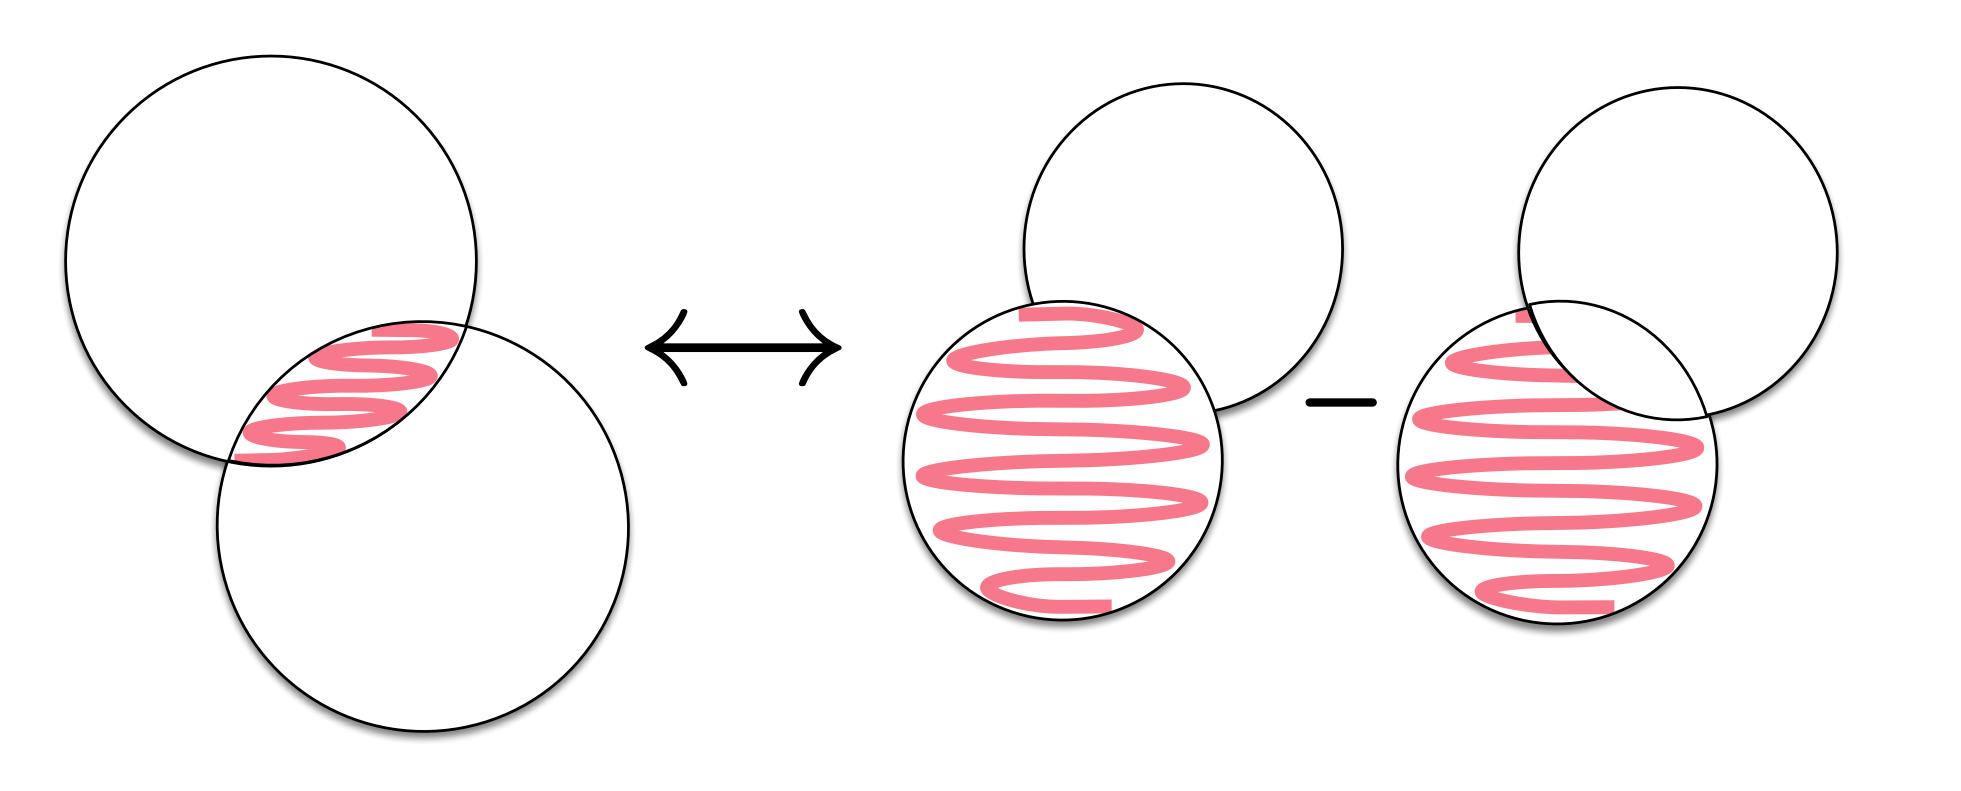
\includegraphics[width=12cm]{images/intersection1.png}
\caption{Venn-Diagram showing the definition of Intersection in terms of Set Difference}
\end{figure}
        
    \vspace{0.1in}
    
     \textbf{Part 4} \\
    Explain the difference between DRC and TRC.
    
    \vspace{0.1in}
        \solution \\
In Tuple Relational Calculus (TRC), the variables typically range over tuples, i.e. they directly represent tuples. On the other hand, in Domain Relational Calculus (DRC), the variables range over domain elements, i.e. field values. In TRC, tuples are semantically equivalent to variables, i.e. field referencing can be used to select tuple parts. On the other hand, in DRC, formal variables are explicit and have to be defined.
    \vspace{0.1in}
    
    
\end{homeworkProblem}   

\begin{homeworkProblem}

\textbf{Part 1} \\

The names of the seas that are deeper than 3000 mt and into which at least one river finally flows.

\vspace{0.1in}
    \solution \\
      
    $<name> \mid \exists depth, rname, river, lake, sea, length, sLong, sLat, mount, sAlt, estLong, estLat \\
    Sea(name, depth) \wedge  \\ River(rname, river, lake, sea, length, sLong, sLat, mount, sAlt, estLong, estLat) \wedge \\ depth > 3000 \wedge sea = name$ 
    \vspace{0.1in}
    
\textbf{Part 2} \\
The names of the groups of islands that consist only of islands that are neither 'volcanic' nor
'coral'.

 \vspace{0.1in}
    \solution \\ \\    
   %SOLUTION
   $<islands> \mid \exists name, area, height, type, long, lat \\
Island(name, islands, area, height, type, long, lat) \wedge \\
type \notin \{volcanic, coral\} \wedge islands \neq \emptyset  $
    \vspace{0.1in}    

\textbf{Part 3} \\
The name of the mountain, the name of the mountains where it belongs to and the name of
the country where the mountain is located for each mountain that is located on an island
that is of type 'coral'.

 
 \vspace{0.1in} 
     \solution \\ \\ 
     %SOLUTION   
     $<moiMountain, mMountains, gmCountry> \mid \exists \\ moiIsland, mHeight, mType, mLong, mLat, \\ iIslands, iArea, iHeight, iType, iLong, iLat, gmProvince \\
mountainOnIsland(moiMountain, moiIsland) \wedge \\ Mountain(moiMountain, mMountains, mHeight, mType, mLong, mLat) \wedge \\ geo\_Mountain(moiMountain, gmCountry, gmProvince)  \wedge \\
Island(moiIsland, iIslands, iArea, iHeight, iType, iLong, iLat) \wedge iType \neq "coral" $

     \vspace{0.1in}

    
\textbf{Part 4} \\
Give the name and country name of all cities with a population higher than 500,000.

 \vspace{0.1in} 
     \solution \\ \\    
    %SOLUTION
   $<cName, coName> \mid \exists cCountry, cProvince, cPopulation, cLong, cLat, \\
   coCapital, coProvince, coArea, coPopulation \\
City(cName, cCountry, cProvince, cPopulation, cLong, cLat)  \wedge \\
Country(cCountry, coName, coCapital, coProvince, coArea, coPopulation) \wedge \\
cPopulation > 500000 $
 
    \vspace{0.1in}
        
\end{homeworkProblem}

\begin{homeworkProblem}
Suppose you have a file of 15,000 pages and eight buffer pages and you are sorting it using general
(external) merge-sort. Please answer the following questions: \\

\textbf{Part 1} \\
How many runs will you produce? Remark: When a file is sorted, in intermediate steps
subfiles are created. Each sorted subfile is called a run. See also slide 35 in Chapter 2.
 \textbf{Note: Detailed solution of Q3 is produced in \textit{Figures 2, 3 and 4.}}
 
 \vspace{0.1in} 
     \solution \\
     %SOLUTION
     \textbf{2189} runs will be produced   
     \vspace{0.1in}
     
 \textbf{Part 2} \\
How many passes will it take to sort the file completely?
 
 \vspace{0.1in} 
     \solution \\ 
    It will take \textbf{5} passes   
     \vspace{0.1in}
     
 \textbf{Part 3} \\
How many buffer pages do you need at least to sort the file in two passes? 

 \vspace{0.1in} 
     \solution \\
     With \textbf{123} buffers, you can sort the file in two passes 
     \vspace{0.1in}
 
 \textbf{Part 4} \\
How many runs and passes would a Two-Way-Sort algorithm take?
 
 \vspace{0.1in} 
     \solution \\
     %SOLUTION
     Two-Way Sort Algorithm will take \textbf{30004} runs and \textbf{15} passes   
     \vspace{0.1in}   
     
\begin{figure}[h]
\centering
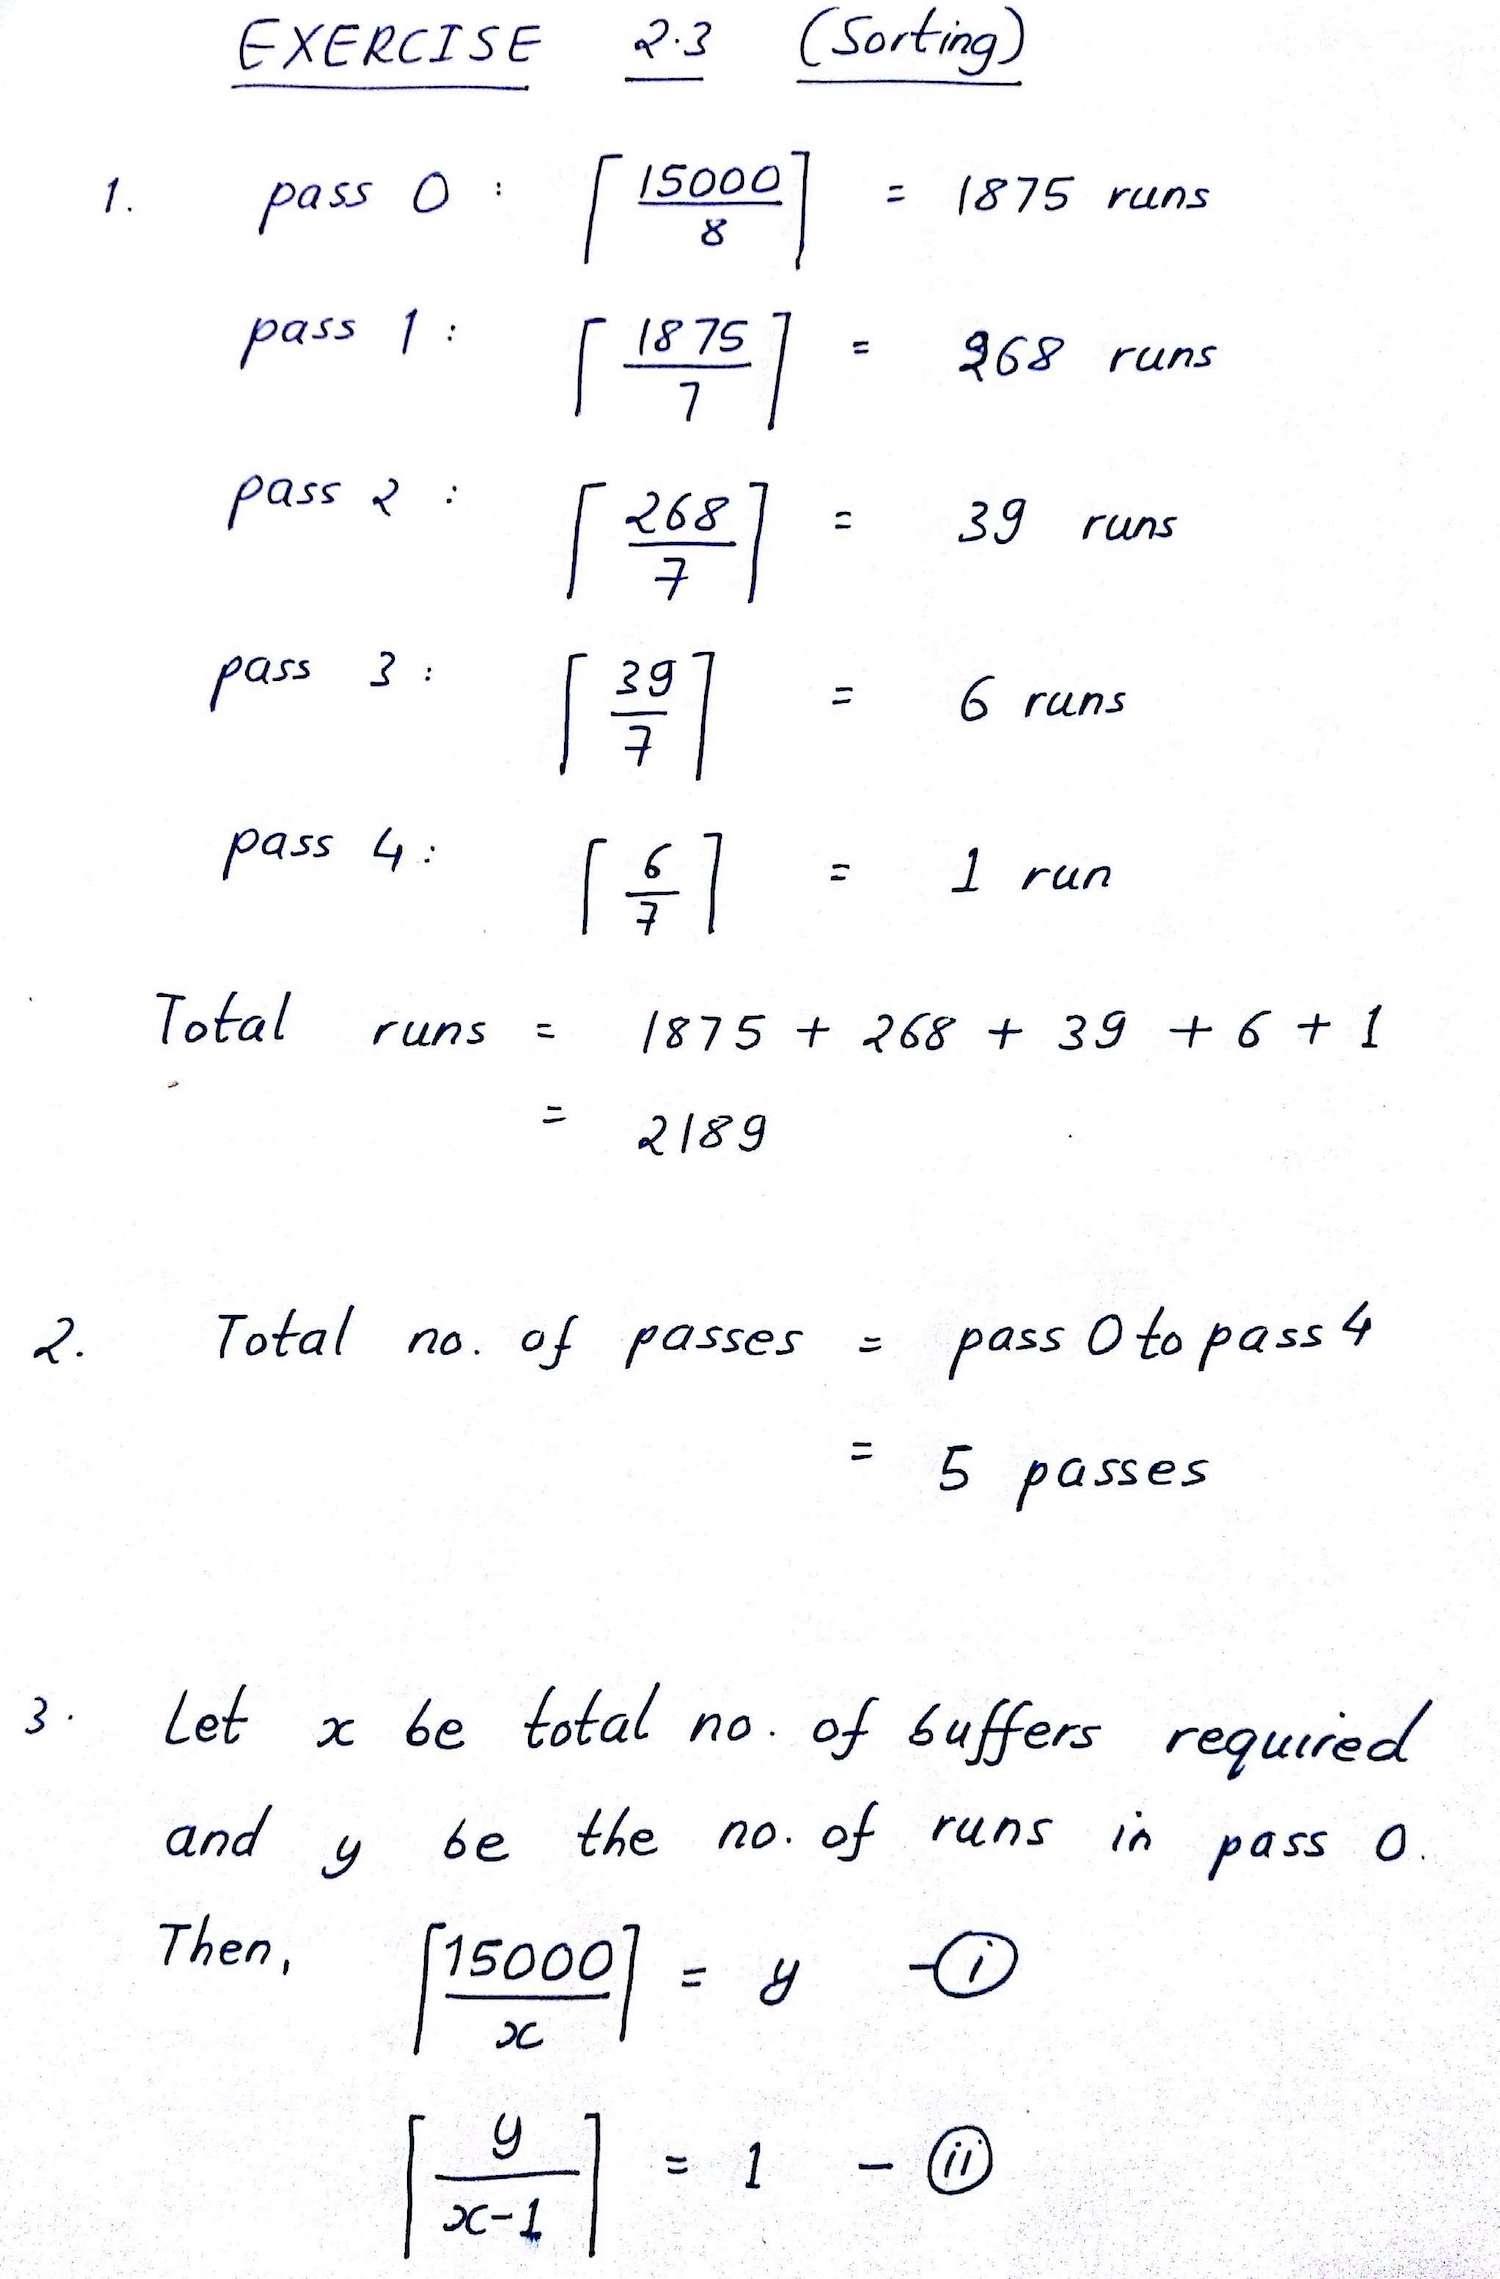
\includegraphics[width=12cm]{images/sol31.jpg}
\caption{Paper-based Solution for Question 3-1}
\end{figure} 

\begin{figure}[h]
\centering
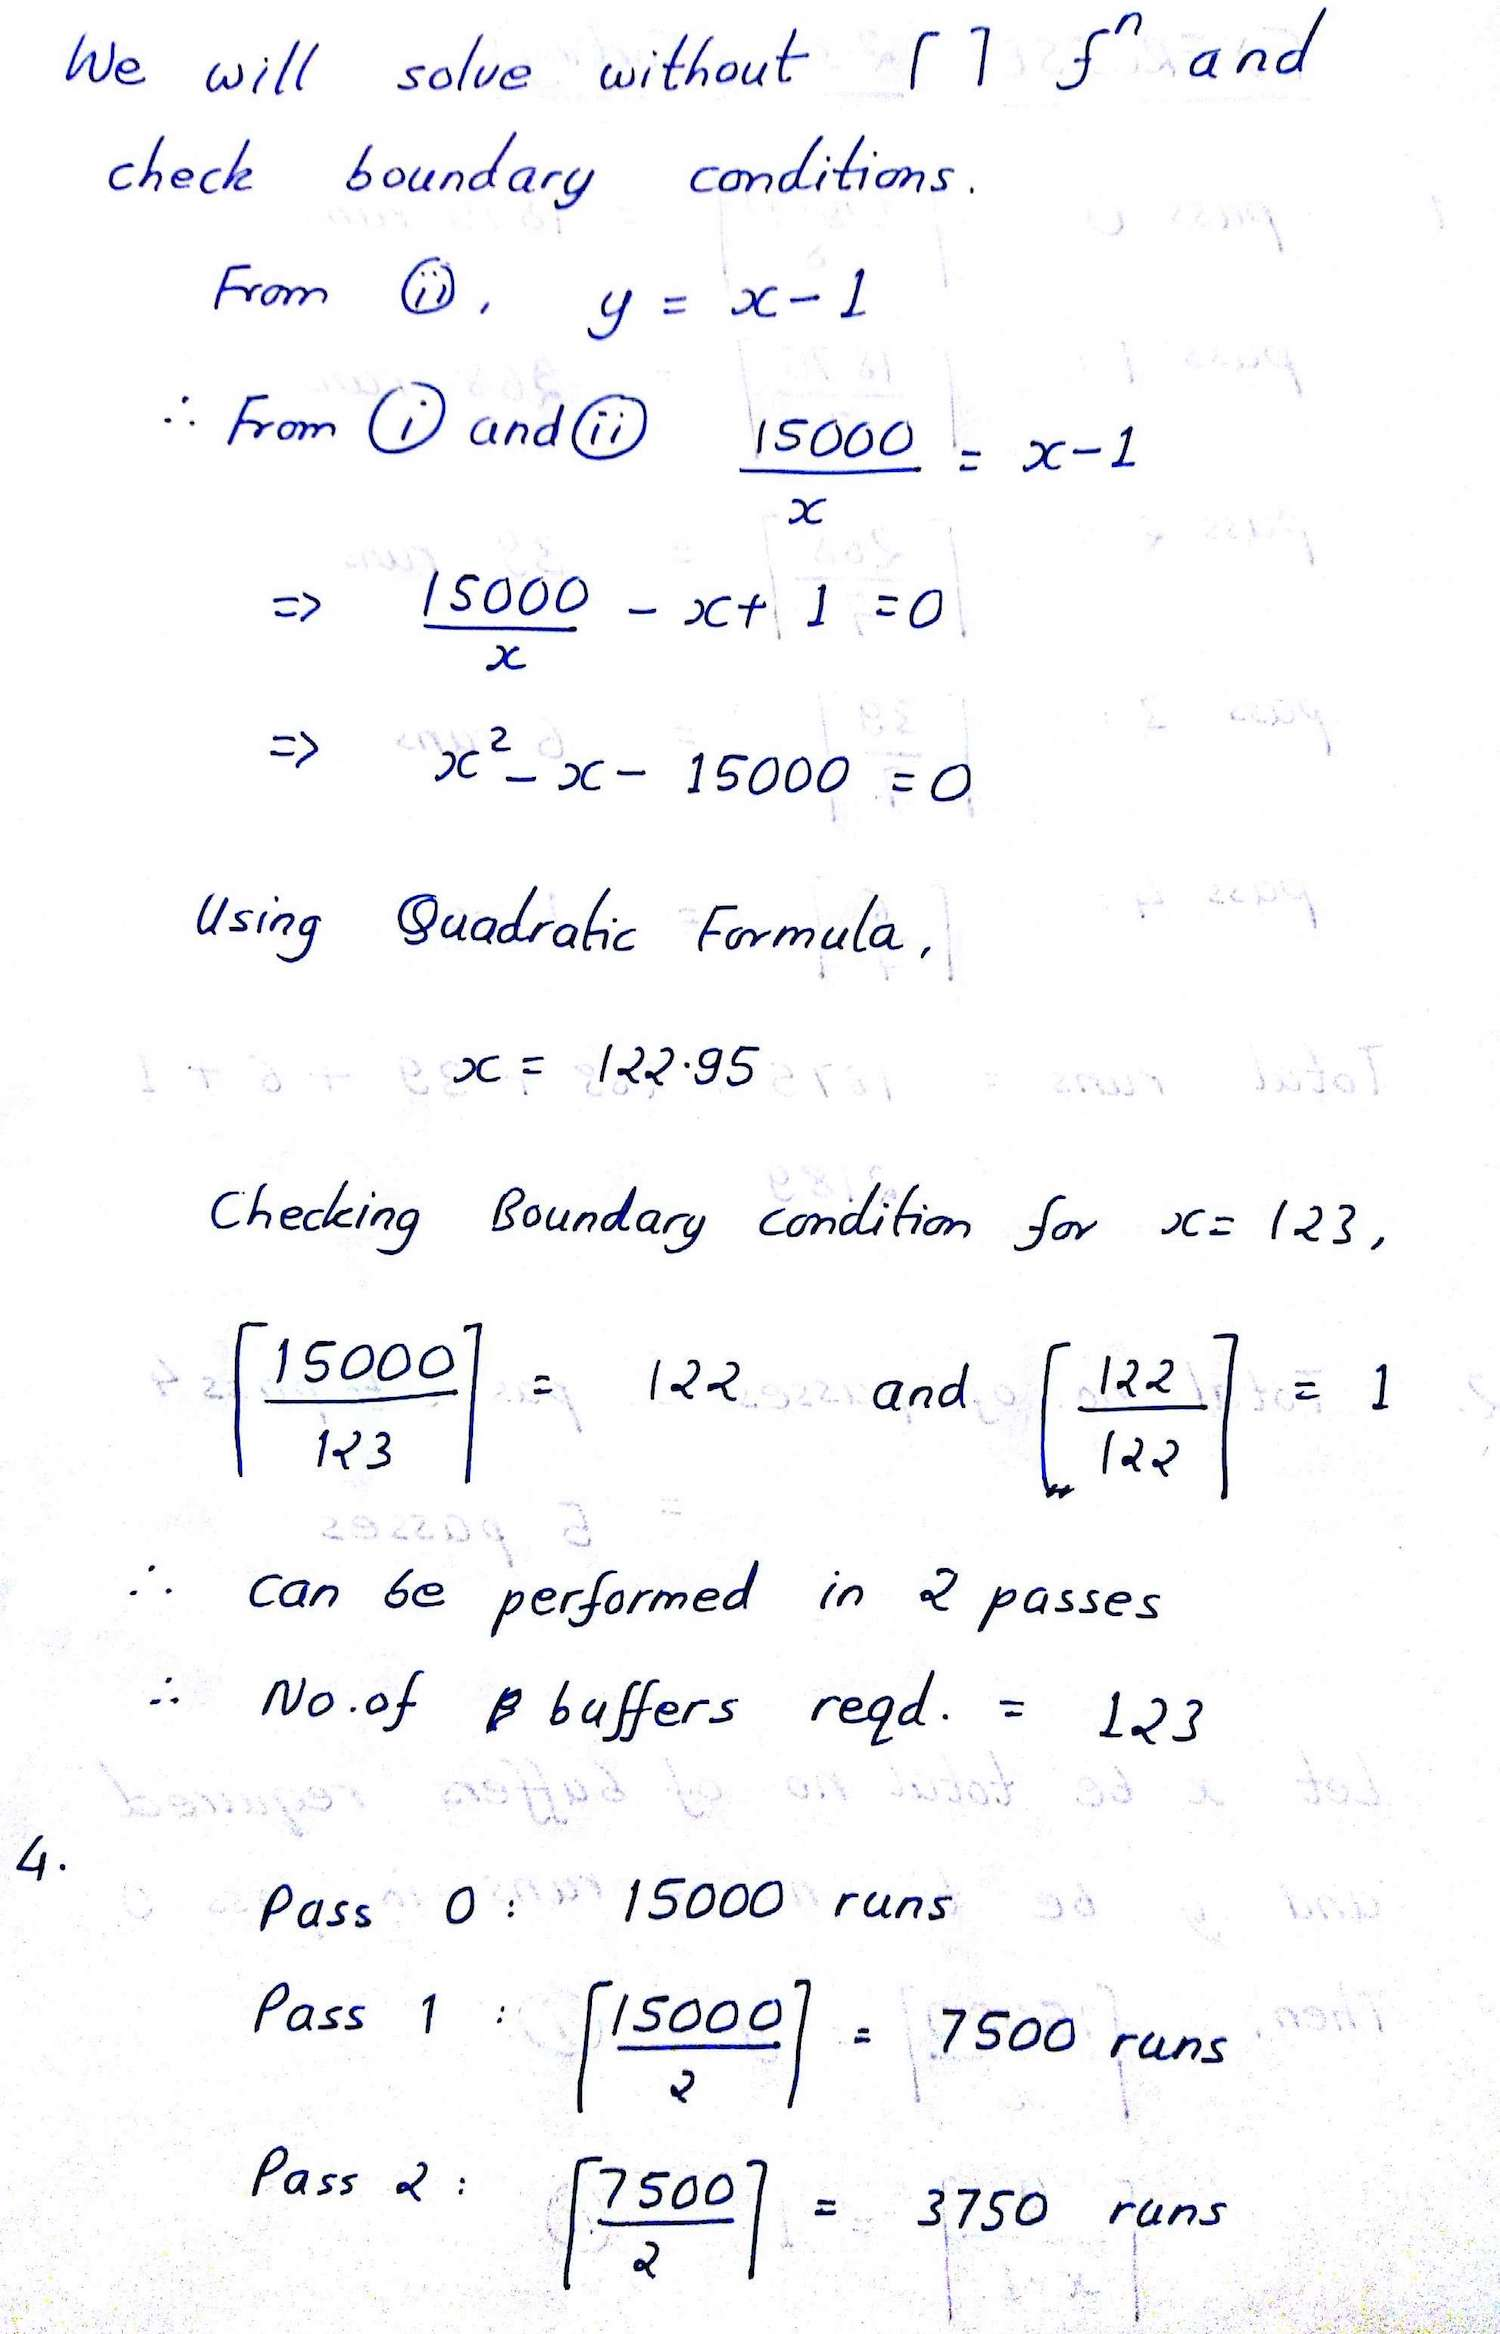
\includegraphics[width=12cm]{images/sol32.jpg}
\caption{Paper-based Solution for Question 3-2}
\end{figure} 

\begin{figure}[h]
\centering
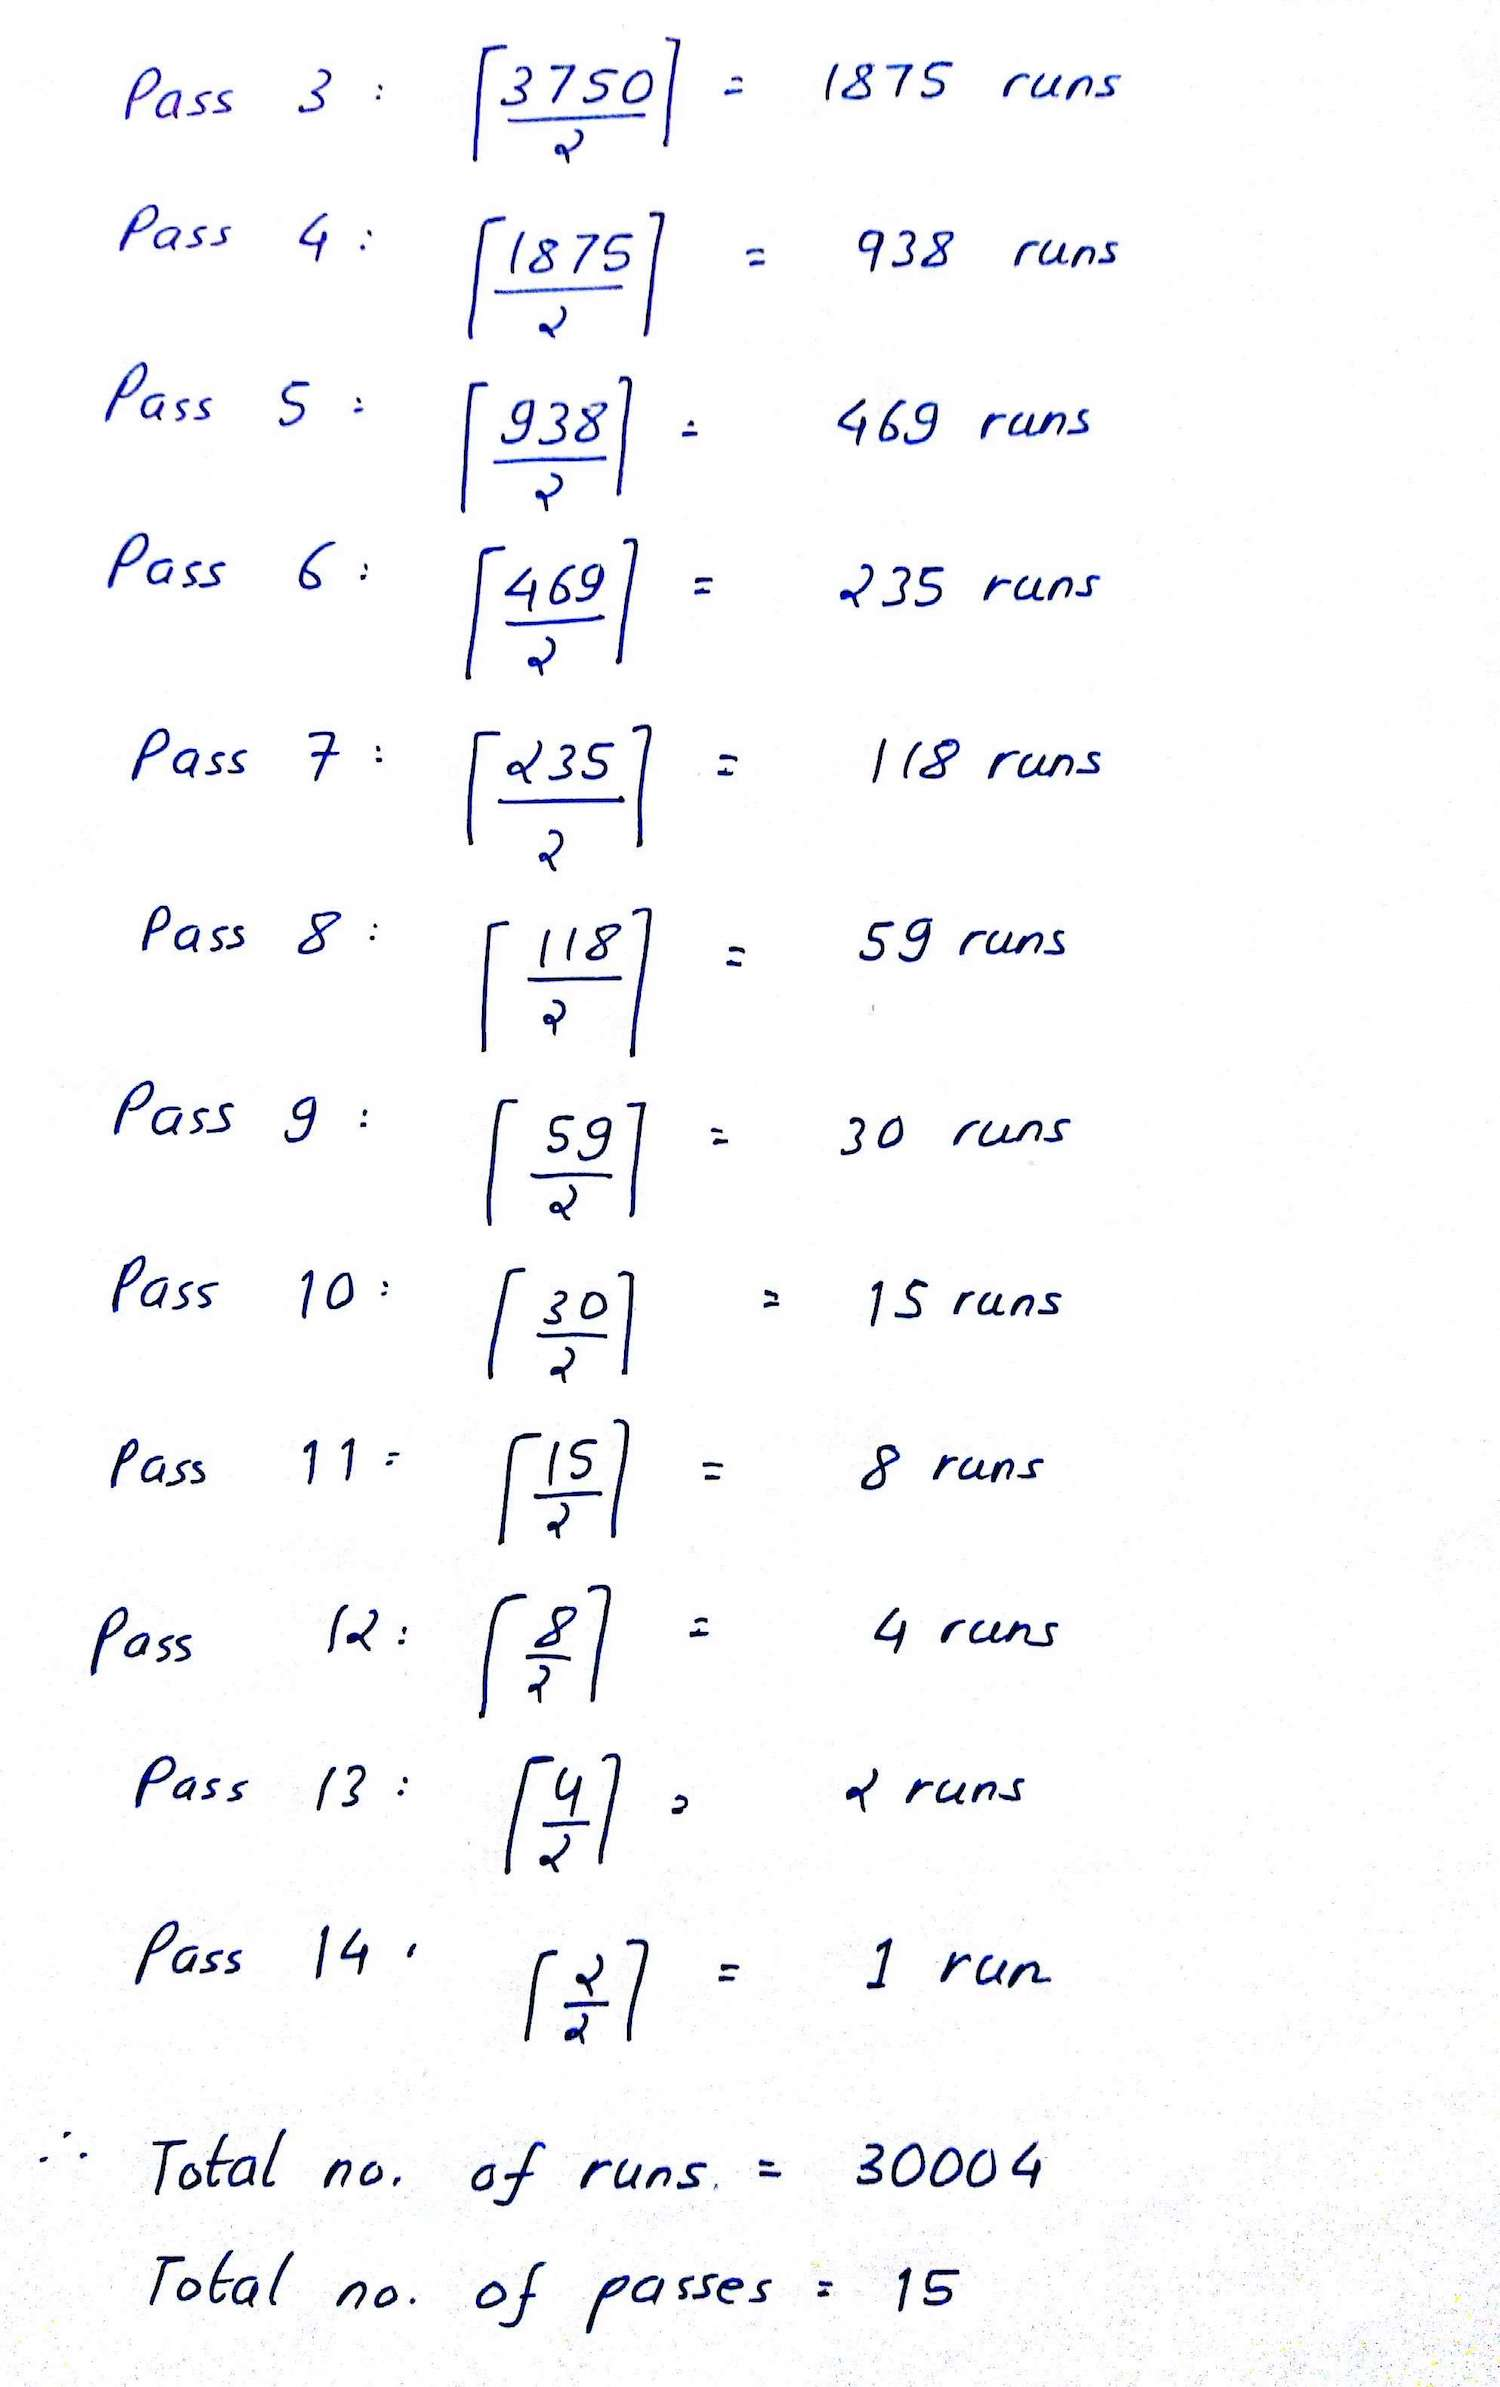
\includegraphics[width=12cm]{images/sol33.jpg}
\caption{Paper-based Solution for Question 3-3}
\end{figure} 

\end{homeworkProblem}

\begin{homeworkProblem}

\textbf{Part 1} \\
Calculate the I/O requirements of a simple nested loop join
 
 \vspace{0.1in} 
     \solution \\ \\ 
     %SOLUTION 
     In the expression below, M and N are the number of pages in the relations Album and Track respectively, $p_M$ and $p_N$ are the number of tuples in each page of the relations. \\
     
     \textbf{M as outer and N as inner relation} \\
     \textbf{Tuple-by-Tuple Simple Nested Loop Join} \\
     $M +  p_M \times M \times N$ \\
     $= 10000 + 100 \times 10000 \times 200000$ \\
     $ = 200000010000 $
          
    \vspace{0.1in}
     \textbf{Page-by-Page Simple Nested Loop Join} \\
     $M + M \times N$ \\
     $= 10000 + 10000 \times 200000$ \\
     $ = 2000010000 $
     
      \vspace{0.1in}
     \textbf{N as outer and M as inner relation} \\
     \textbf{Tuple-by-Tuple Simple Nested Loop Join} \\
     $N +  p_N \times N \times M$ \\
     $= 200000 + 80 \times 200000 \times 10000$ \\
     $ = 160000200000 $
          
    \vspace{0.1in}
     \textbf{Page-by-Page Simple Nested Loop Join} \\
     $M + M \times N$ \\
     $= 200000 + 200000 \times 10000$ \\
     $ = 2000200000 $
     \vspace{0.1in}
     
 \textbf{Part 2} \\
Calculate the I/O requirements of a block nested loop join
 
\vspace{0.1in} 
     \solution \\ \\ 
     %SOLUTION
     Block nested join for 16 buffers: \\
     
      \textbf{M as outer and N as inner relation} \\
     $ 10000 + \lceil \frac{10000}{14} \rceil \times 200000$
     $ = 143010000 $   
     \vspace{0.1in}
     
      \textbf{N as outer and M as inner relation} \\
      $ 200000 + \lceil \frac{200000}{14} \rceil \times 10000$
     $ = 143060000 $   
     \vspace{0.1in}
     
 \textbf{Part 3} \\
Explain the differences between the two algorithms. What are the similarities and differences? How does the block nested loop join reduce I/O costs?
 
 \vspace{0.1in} 
     \solution \\ \\ 
     %SOLUTION
     Tuple-at-a-time Simple Nested Loop Join scans outer relation and then for each tuple, it scans the entire inner relation. On the other hand, the page-at-a-time Simple Nested Loop Join will load the outer relation page-by-page, and then the inner relation for each page. The Block Nested Loop Join, on the other hand, scans entire inner relation for each block of pages in the outer relation. Therefore, the I/O cost of Block Nested Loop Join is lower than cost of both the Simple Nested Loop Joins. 
Moreover, the other important difference is number of buffer pages used in the algorithms. Both tuple-at-a-time nested loop and page-at-time nested loop join use 3 buffer pages to perform the join operation. 1 page as input buffer to scan outer relation,1 page as input buffer to scan inner relation  and 1 page as output buffer. Totally, 3 pages are needed for simple nested loop join. However, block nested loop join uses 1 page as input buffer to scan inner relation S and 1 page as output buffer. The other remaining buffer pages are used to load the blocks of the outer relation R. In this case, 1 buffer page is used as input buffer to scan inner relation  and 1 page as output buffer. Remaining 14 buffer pages are used to block outer relation . As seen, block nested loop join uses entire available buffer pages in the algorithm that means more efficient usage of buffer pages and causing performance increases and decreasing I/O cost. 

The similarities can be indicated as outer-inner relation usage, buffer usage and loop operations in the algorithms. 

     \vspace{0.1in}
     
\end{homeworkProblem}
     
\begin{homeworkProblem}
Given is a relation with 50.000 records. Each page for a node in a B+ tree can hold 20 pointers
to records or pages. A data page can store 20 records. \\

 \textbf{Part 1} \\
Assume that each node is 70 \% full. What is the height of the B+-tree? 

 \vspace{0.1in} 
     \solution \\ \\ 
     %SOLUTION  
     Given that the B+Tree can hold 20 pointers to pages. However, the B+ Tree has 70\% occupancy. Therefore, number of effective pointers to pages that the tree can hold,
     \begin{center} $ \implies 0.7 \times 20 = 14$ \end{center} 
Our B+ Tree can now be represented as Table 1

\begin{table}[]
\centering
\begin{tabular}{|l|l|l|l|}
\hline
Level    & Node & Entries & No. of Pointers \\ \hline
0 (Root) & 1    & 13      & 14              \\ \hline
1        & 14   & 182     & 196             \\ \hline
2        & 196  & 2548    & 2744         \\ \hline  
\end{tabular}
\caption{Different Levels of the B+ Tree}
\label{B+ Tree}
\end{table}

We have 2744 addresses in Level 2 already, which is more than 2500 pointers to pages required in the relations. \\
Therefore, the B-Tree has a depth of \textbf{3}.
Our B+ Tree has a depth of \textbf{3}
 \vspace{0.1in}
     
 \textbf{Part 2} \\
What are the I/O costs for an equality selection on a non-key attribute for the following
cases?

\begin{enumerate}[label = (\alph*)]
\item with a clustered B+-tree of height 3 (matching records are located in one page);
 
 \vspace{0.1in} 
     \solution \\ \\ 
     %SOLUTION
     The clustered index will guide the search, and after the end of the B+ tree traversal, we will need to input the correct page which contains our desired result. Therefore, total I/O is for the tree traversal and retrieving the correct page, i.e. 3 I/Os + 1 I/O = 4.
     Hence, total number of I/Os = \textbf{4} I/Os
     \vspace{0.1in}
     
\item without any index, nor is the file sorted on the attribute occurring in selection;

\vspace{0.1in} 
     \solution \\ \\ 
     %SOLUTION 
     Total number of pages at the leaf node = 2500
    If we consider that all pages need to be scanned, then the I/O costs will be \textbf{2500} I/Os. \\
    However, assuming, on an average that half the total number of pages need to be searched to find the equality results, it gives a total of 1250 I/Os.
          
     \vspace{0.1in}
     
\item with an unclustered B+-tree index of height 4, and there are 2 matching records;

\vspace{0.1in} 
     \solution \\ \\ 
     4 I/Os to traverse the tree + 2 I/Os to retrieve the matching records = \textbf{6} I/Os 
     \vspace{0.1in}

\item with an unclustered B+-tree of height 5 and three tenth of the records match the
selection.

\vspace{0.1in} 
\solution \\ \\ 
     %SOLUTION
     No. of matching records = $\frac{3}{10} \times 50000 = 15000$ records \\
     In the worst case, we need to do 15000 page I/Os, one for each record. Plus the I/Os for traversing the tree. Therefore, a total of 15000 I/Os + 5 I/Os = \textbf{15005} I/Os.   
     \vspace{0.1in}

\end{enumerate}
\end{homeworkProblem}

\end{document}
\documentclass[12pt]{article}

\usepackage{fancyhdr}
\usepackage{extramarks}
\usepackage{amsmath}
\usepackage{amsthm}
\usepackage{amsfonts}
\usepackage{tikz}
\usepackage[plain]{algorithm}
\usepackage{algpseudocode}
\usepackage[export]{adjustbox}
\usepackage[latin1]{inputenc}           %For German characters
\usepackage{enumitem}               %For changing enumeration character
\usepackage{listings}               %For code
\usepackage{csquotes}
\usepackage{graphicx}               %For graphics e.g, images

\usetikzlibrary{automata,positioning}

%
% Basic Document Settings
%

\topmargin=-0.45in
\evensidemargin=0in
\oddsidemargin=0in
\textwidth=6.5in
\textheight=9.0in
\headsep=0.25in

\linespread{1.1}

\pagestyle{fancy}
\lhead{\hmwkAuthorName}
\chead{\hmwkClass\ : \hmwkTitle}
\rhead{\firstxmark}
\lfoot{\lastxmark}
\cfoot{\thepage}

\renewcommand\headrulewidth{0.4pt}
\renewcommand\footrulewidth{0.4pt}

\setlength\parindent{0pt}

%
% Create Problem Sections
%

\newcommand{\enterProblemHeader}[1]{
    \nobreak\extramarks{}{Problem \arabic{#1} continued on next page\ldots}\nobreak{}
    \nobreak\extramarks{Problem \arabic{#1} (continued)}{Problem \arabic{#1} continued on next page\ldots}\nobreak{}
}

\newcommand{\exitProblemHeader}[1]{
    \nobreak\extramarks{Problem \arabic{#1} (continued)}{Problem \arabic{#1} continued on next page\ldots}\nobreak{}
    \stepcounter{#1}
    \nobreak\extramarks{Problem \arabic{#1}}{}\nobreak{}
}

\setcounter{secnumdepth}{0}
\newcounter{partCounter}
\newcounter{homeworkProblemCounter}
\setcounter{homeworkProblemCounter}{1}
\nobreak\extramarks{Problem \arabic{homeworkProblemCounter}}{}\nobreak{}

%
% Homework Problem Environment
%
% This environment takes an optional argument. When given, it will adjust the
% problem counter. This is useful for when the problems given for your
% assignment aren't sequential. See the last 3 problems of this template for an
% example.
%
\newenvironment{homeworkProblem}[1][-1]{
    \ifnum#1>0
        \setcounter{homeworkProblemCounter}{#1}
    \fi
    \section{Problem \arabic{homeworkProblemCounter}}
    \setcounter{partCounter}{1}
    \enterProblemHeader{homeworkProblemCounter}
}{
    \exitProblemHeader{homeworkProblemCounter}
}

%
% Homework Details
%   - Title
%   - Due date
%   - Class
%   - Section/Time
%   - Instructor
%   - Author
%

\newcommand{\hmwkTitle}{Assignment\ \#2}
\newcommand{\hmwkDueDate}{November 15, 2016}
\newcommand{\hmwkClass}{Implementation of Databases}
\newcommand{\hmwkAuthorName}{Sanchit Alekh}
\newcommand{\hmwkClassTime}{MSc. Software Systems Engineering}
\newcommand{\hmwkClassInstructor}{Universitätsprofessor Dr. rer. pol. Matthias Jarke}
\newcommand{\hmwkClassInstructors}{Dr. rer. nat. Christoph Quix}

%
% Title Page
%



\title{
   \begin{center}
   \vspace*{-20mm}
   
\includegraphics[width=0.4\textwidth, right]{images/rwth_logo.png}
   \\
   \vspace*{3cm}
    \textmd{\textbf{\hmwkClass}}\\
    \textmd{\textbf{\hmwkTitle}}\\
    \normalsize\vspace{0.1in}\small{Due\ on\ \hmwkDueDate } \\
    \vspace{0.1in}\large{\textit{\hmwkClassInstructor}} \\
    \vspace{0.1in}\large{\textit{\hmwkClassInstructors}} \\
    \vspace{3in}
     \textbf{Submitted by:} \\
     \vspace{0.25in}
    \large{Sanchit Alekh, Idil Esen Zülfikar, Nihal Hegde} \\
    %\author{\textbf{\hmwkAuthorName}}
    \vspace{0.1in} \large{\textit{\hmwkClassTime}} \\
    %\vspace{0.1in} \large{\textit{Matrikelnummer : 359831}}
    \end{center}
    }


\date{}

\renewcommand{\part}[1]{\textbf{\large Part \Alph{partCounter}}\stepcounter{partCounter}\\}

%
% Various Helper Commands
%

% Useful for algorithms
\newcommand{\alg}[1]{\textsc{\bfseries \footnotesize #1}}

% For derivatives
\newcommand{\deriv}[1]{\frac{\mathrm{d}}{\mathrm{d}x} (#1)}

% For partial derivatives
\newcommand{\pderiv}[2]{\frac{\partial}{\partial #1} (#2)}

% Integral dx
\newcommand{\dx}{\mathrm{d}x}

% Alias for the Solution section header
\newcommand{\solution}{\textbf{\large Solution}}

% Probability commands: Expectation, Variance, Covariance, Bias
\newcommand{\E}{\mathrm{E}}
\newcommand{\Var}{\mathrm{Var}}
\newcommand{\Cov}{\mathrm{Cov}}
\newcommand{\Bias}{\mathrm{Bias}}

\begin{document}

\maketitle

\pagebreak

\begin{homeworkProblem}
    
    \textbf{Part 1} \\
    Variants of relational algebra are used internally in DBMS to represent queries and query evaluation plans. Please explain, why relational algebra is suitable for this?
    
    \vspace{0.1in}
    \solution \\
    One of the most desirable properties of Relational Algebra is that queries are composed using a collection of operators, and every operator accepts one or two relation instances as arguments and returns a relation instance as the result. This property makes extremely easy and efficient to compose operators to form a complex query. A relational algebra expression can be recursively defined to be a relation, a unary algebra operator applied to a single expression, or a binary algebra operator applied to two expressions. 
This procedural nature of relational algebra is the main reason why it is used internally in DBMS to represent queries and evaluation plans. The approach allows us to think of an algebra expression as an imperative execution plan for a declarative SQL query. It can be used for evaluating a query, and relational systems in fact use algebra expressions to represent query evaluation plans.
        
    \vspace{0.1in}
    
    \textbf{Part 2} \\
    What does \enquote{relational completeness} mean (in your own words, please)? Show that SQL is
relationally complete by enumerating SQL constructs corresponding to selection, projection,
cartesian product, union, and difference.
    
    \vspace{0.1in}
    \solution \\
    \enquote{Relational Completeness} of a query methodology means that each and every query that can be expressed using that methodology, can also be expressed as a relational algebra query. In this case, SQL is referred to as \enquote*{Relationally Complete} because every legal construct in SQL can be expressed as a Relational Algebra query.
        
These are the examples of Relational Algebra expressions and their equivalent expressions in SQL. The following examples are derived from the \textit{Mondial} database.

\begin{itemize}

\item \textbf{SELECTION} \\
Relational Algebra: $ \sigma_{Area > 650} (Island)$ \\
SQL:  \textit{Select * From Island Where Area $>$ 650;}

\item \textbf{PROJECTION} \\
Relational Algebra: $ \pi_{Name, Islands, Area, Height} (Island)$ \\
SQL: \textit{Select Name, Islands, Area, Height From Island;}

\item \textbf{CARTESIAN PRODUCT} \\
Relational Algebra:  $ Island \times islandIn$ \\
SQL: \textit{Select * From Island CROSS JOIN islandIn;}

\item \textbf{UNION} \\
Relational Algebra:  $ \pi_{name} (Desert) \cup \pi_{name} (geo\_Desert)$ \\
SQL: \textit{Select name From Desert or Select name From geo\_Desert}

\item \textbf{SET DIFFERENCE} \\
Relational Algebra: $ \pi_{name} (\sigma_{height > 5000} (Mountain)) - \pi_{name}( \sigma_{type > 'volcanic')} (Mountain) $ \\
SQL: \textit{Select name From Mountain where height $>$ 5000 MINUS Select name From Mountain where type='volcanic'}
\end{itemize}
        
    \vspace{0.1in}
        
     \textbf{Part 3} \\
    Explain how the intersection operator is used in relational algebra. What is important for
its usage? Is it omittable (i.e., could you express it by other operators)? If so, please give
the corresponding relational algebra.
    
    \vspace{0.1in}
    \solution \\
    The \enquote*{Intersection} operator is represented in Relational Algebra with the help of the $\cap$ symbol. Although it is not a fundamental set-operator, it is an extremely widely used operation, and it is helpful to define it separately. An example use of the intersection operator is as follows:
    
    \begin{center} $ \pi_{name} (Desert) \cap \pi_{name} (geo\_Desert) $ \end{center}
    
The important condition for using the \textit{Intersection} operator is that the two sets which have to be intersected must be \textit{union-compatible}. This follows from the fact that intersection is defined in terms of set difference.

Yes, Intersection is not a fundamental set-operator, and it can be expressed in terms of the set-difference operator. Therefore, it is omittable. A general expression for the intersection operator in terms of the set-difference operator is:

    \begin{center} $ A \cup B \leftrightarrow A \setminus ( A \setminus B) $ \end{center}
    
Therefore, the example Relational Algebra query illustrated above can be represented by the equivalent query without the use of set-intersection as follows:

    \begin{center} $ \pi_{name} (Desert) - (\pi_{name} (Desert) - \pi_{name} (geo\_Desert))$ \end{center}
    
\begin{figure}[h]
\centering
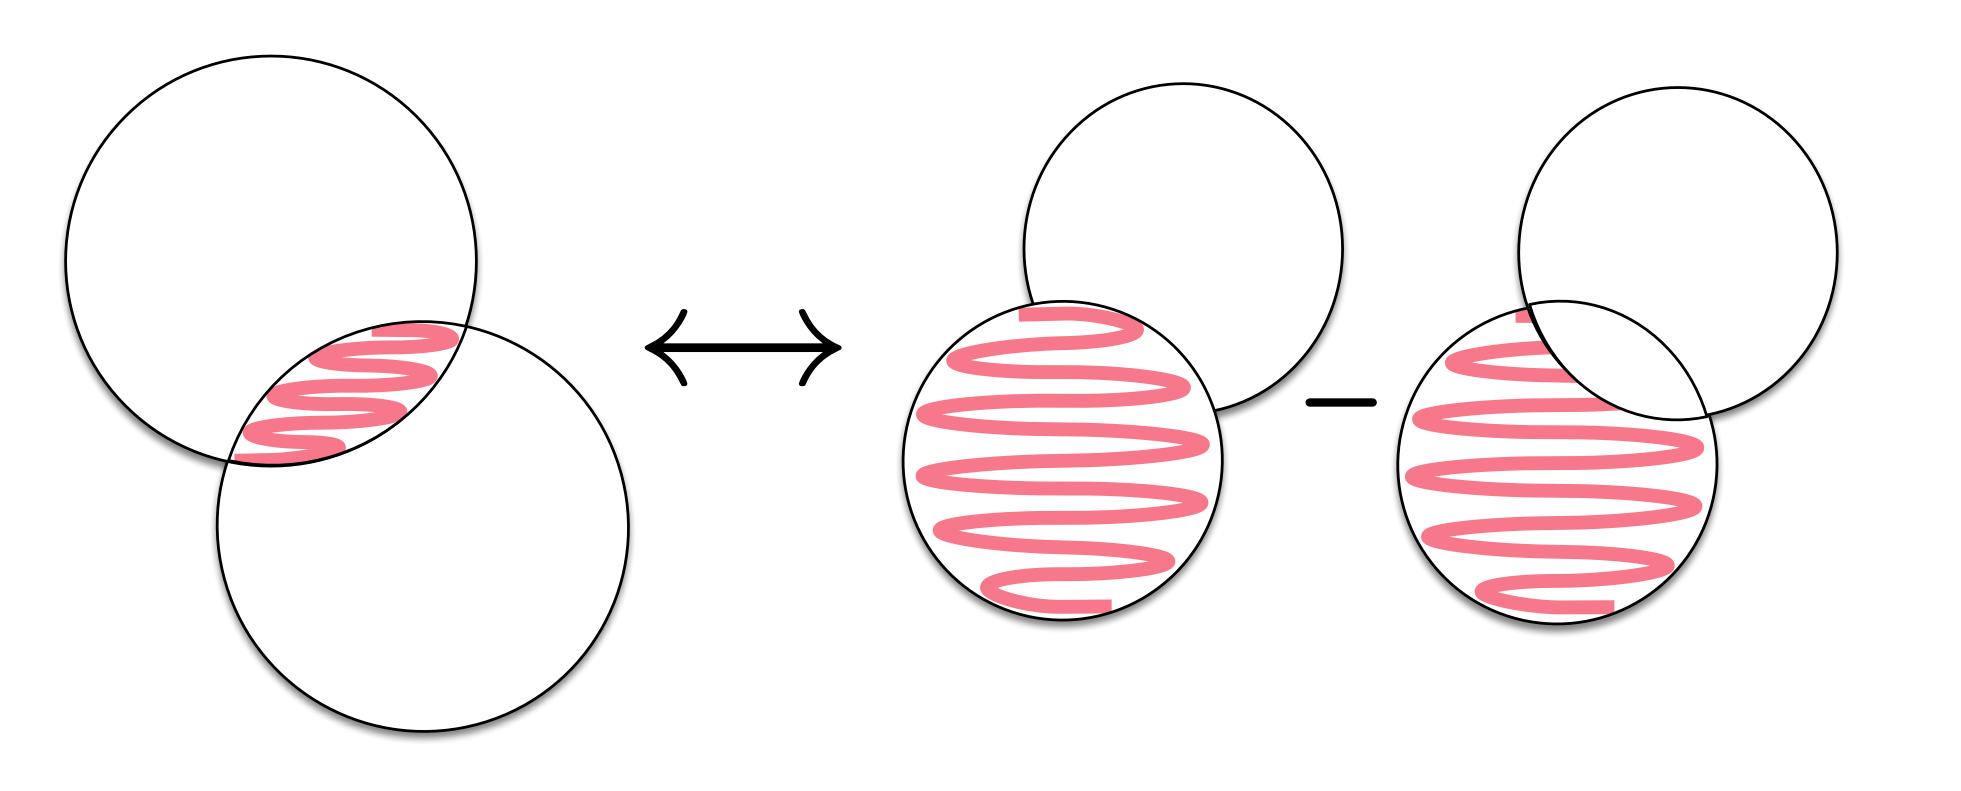
\includegraphics[width=12cm]{images/intersection1.png}
\caption{Venn-Diagram showing the definition of Intersection in terms of Set Difference}
\end{figure}
        
    \vspace{0.1in}
    
     \textbf{Part 4} \\
    Explain the difference between DRC and TRC.
    
    \vspace{0.1in}
        \solution \\
In Tuple Relational Calculus (TRC), the variables typically range over tuples, i.e. they directly represent tuples. On the other hand, in Domain Relational Calculus (DRC), the variables range over domain elements, i.e. field values. In TRC, tuples are semantically equivalent to variables, i.e. field referencing can be used to select tuple parts. On the other hand, in DRC, formal variables are explicit and have to be defined.
    \vspace{0.1in}
    
    
\end{homeworkProblem}   

\begin{homeworkProblem}

\textbf{Part 1} \\

The names of the seas that are deeper than 3000 mt and into which at least one river finally flows.

\vspace{0.1in}
    \solution \\
      
    $<name> \mid \exists depth, rname, river, lake, sea, length, sLong, sLat, mount, sAlt, estLong, estLat \\
    Sea(name, depth) \wedge  \\ River(rname, river, lake, sea, length, sLong, sLat, mount, sAlt, estLong, estLat) \wedge \\ depth > 3000 \wedge sea = name$ 
    \vspace{0.1in}
    
\textbf{Part 2} \\
The names of the groups of islands that consist only of islands that are neither 'volcanic' nor
'coral'.

 \vspace{0.1in}
    \solution \\ \\    
   %SOLUTION
   $<islands> \mid \exists name, area, height, type, long, lat \\
Island(name, islands, area, height, type, long, lat) \wedge \\
type \notin \{volcanic, coral\} \wedge islands \neq \emptyset  $
    \vspace{0.1in}    

\textbf{Part 3} \\
The name of the mountain, the name of the mountains where it belongs to and the name of
the country where the mountain is located for each mountain that is located on an island
that is of type 'coral'.

 
 \vspace{0.1in} 
     \solution \\ \\ 
     %SOLUTION   
     $<moiMountain, mMountains, gmCountry> \mid \exists \\ moiIsland, mHeight, mType, mLong, mLat, \\ iIslands, iArea, iHeight, iType, iLong, iLat, gmProvince \\
mountainOnIsland(moiMountain, moiIsland) \wedge \\ Mountain(moiMountain, mMountains, mHeight, mType, mLong, mLat) \wedge \\ geo\_Mountain(moiMountain, gmCountry, gmProvince)  \wedge \\
Island(moiIsland, iIslands, iArea, iHeight, iType, iLong, iLat) \wedge iType \neq "coral" $

     \vspace{0.1in}

    
\textbf{Part 4} \\
Give the name and country name of all cities with a population higher than 500,000.

 \vspace{0.1in} 
     \solution \\ \\    
    %SOLUTION
   $<cName, coName> \mid \exists cCountry, cProvince, cPopulation, cLong, cLat, \\
   coCapital, coProvince, coArea, coPopulation \\
City(cName, cCountry, cProvince, cPopulation, cLong, cLat)  \wedge \\
Country(cCountry, coName, coCapital, coProvince, coArea, coPopulation) \wedge \\
cPopulation > 500000 $
 
    \vspace{0.1in}
        
\end{homeworkProblem}

\begin{homeworkProblem}
Suppose you have a file of 15,000 pages and eight buffer pages and you are sorting it using general
(external) merge-sort. Please answer the following questions: \\

\textbf{Part 1} \\
How many runs will you produce? Remark: When a file is sorted, in intermediate steps
subfiles are created. Each sorted subfile is called a run. See also slide 35 in Chapter 2.
 \textbf{Note: Detailed solution of Q3 is produced in \textit{Figures 2, 3 and 4.}}
 
 \vspace{0.1in} 
     \solution \\
     %SOLUTION
     \textbf{2189} runs will be produced   
     \vspace{0.1in}
     
 \textbf{Part 2} \\
How many passes will it take to sort the file completely?
 
 \vspace{0.1in} 
     \solution \\ 
    It will take \textbf{5} passes   
     \vspace{0.1in}
     
 \textbf{Part 3} \\
How many buffer pages do you need at least to sort the file in two passes? 

 \vspace{0.1in} 
     \solution \\
     With \textbf{123} buffers, you can sort the file in two passes 
     \vspace{0.1in}
 
 \textbf{Part 4} \\
How many runs and passes would a Two-Way-Sort algorithm take?
 
 \vspace{0.1in} 
     \solution \\
     %SOLUTION
     Two-Way Sort Algorithm will take \textbf{30004} runs and \textbf{15} passes   
     \vspace{0.1in}   
     
\begin{figure}[h]
\centering
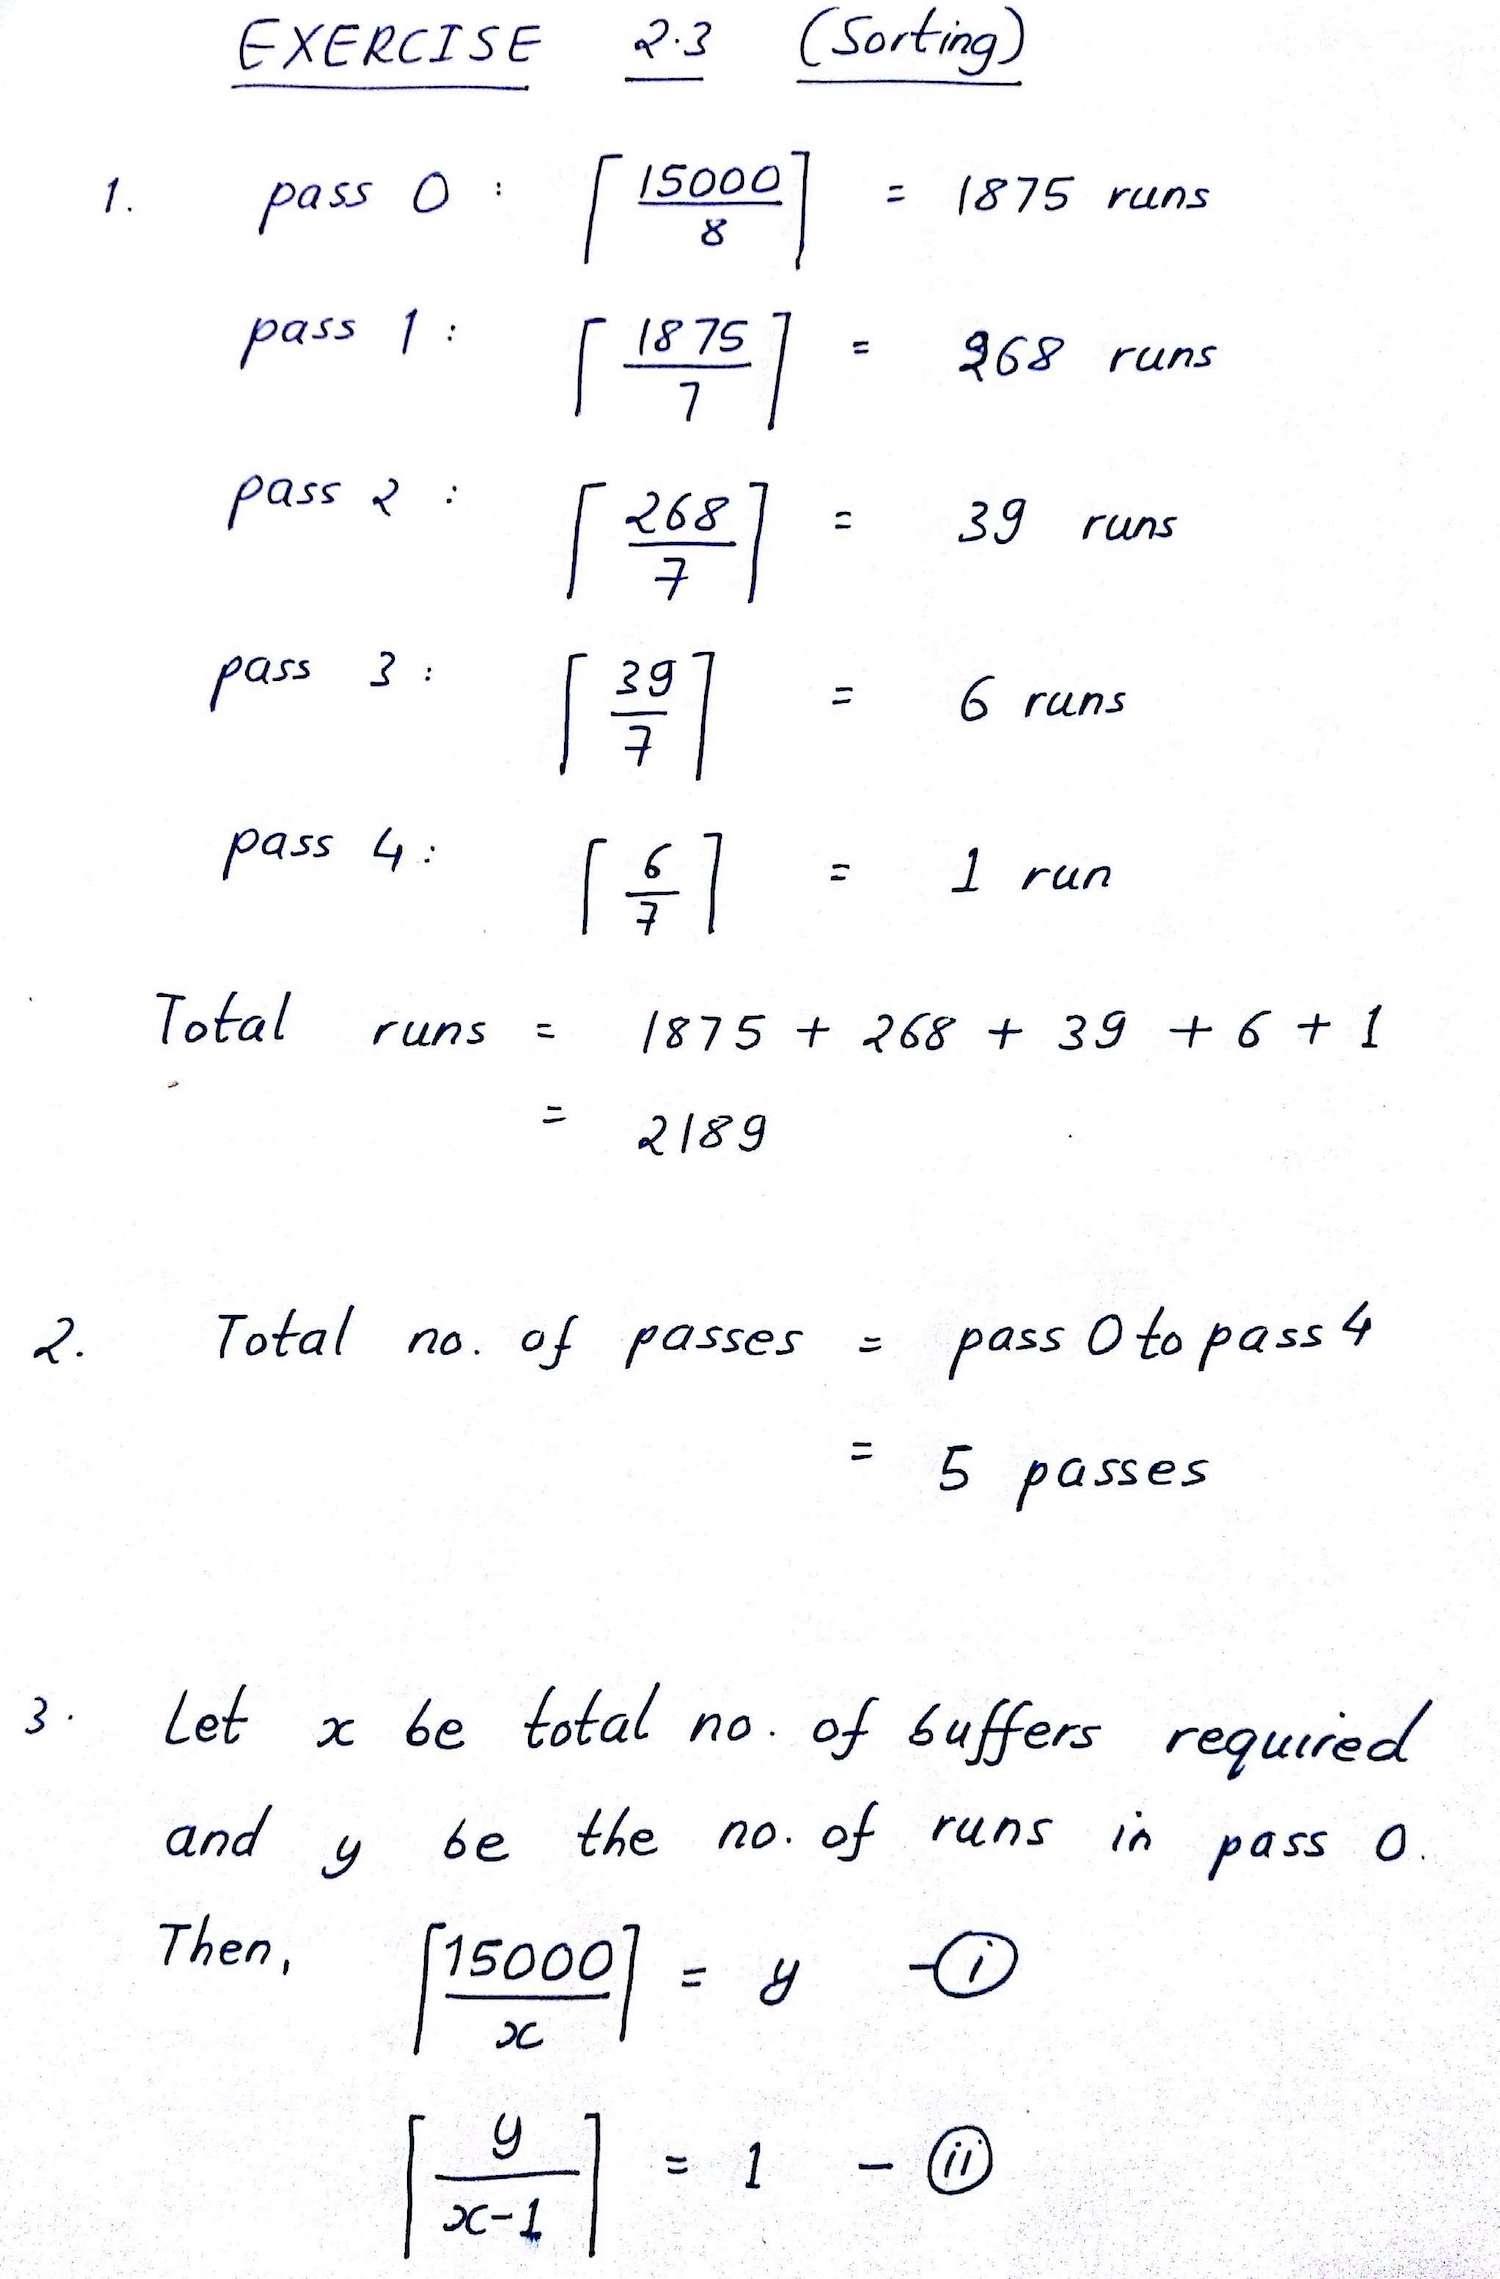
\includegraphics[width=12cm]{images/sol31.jpg}
\caption{Paper-based Solution for Question 3-1}
\end{figure} 

\begin{figure}[h]
\centering
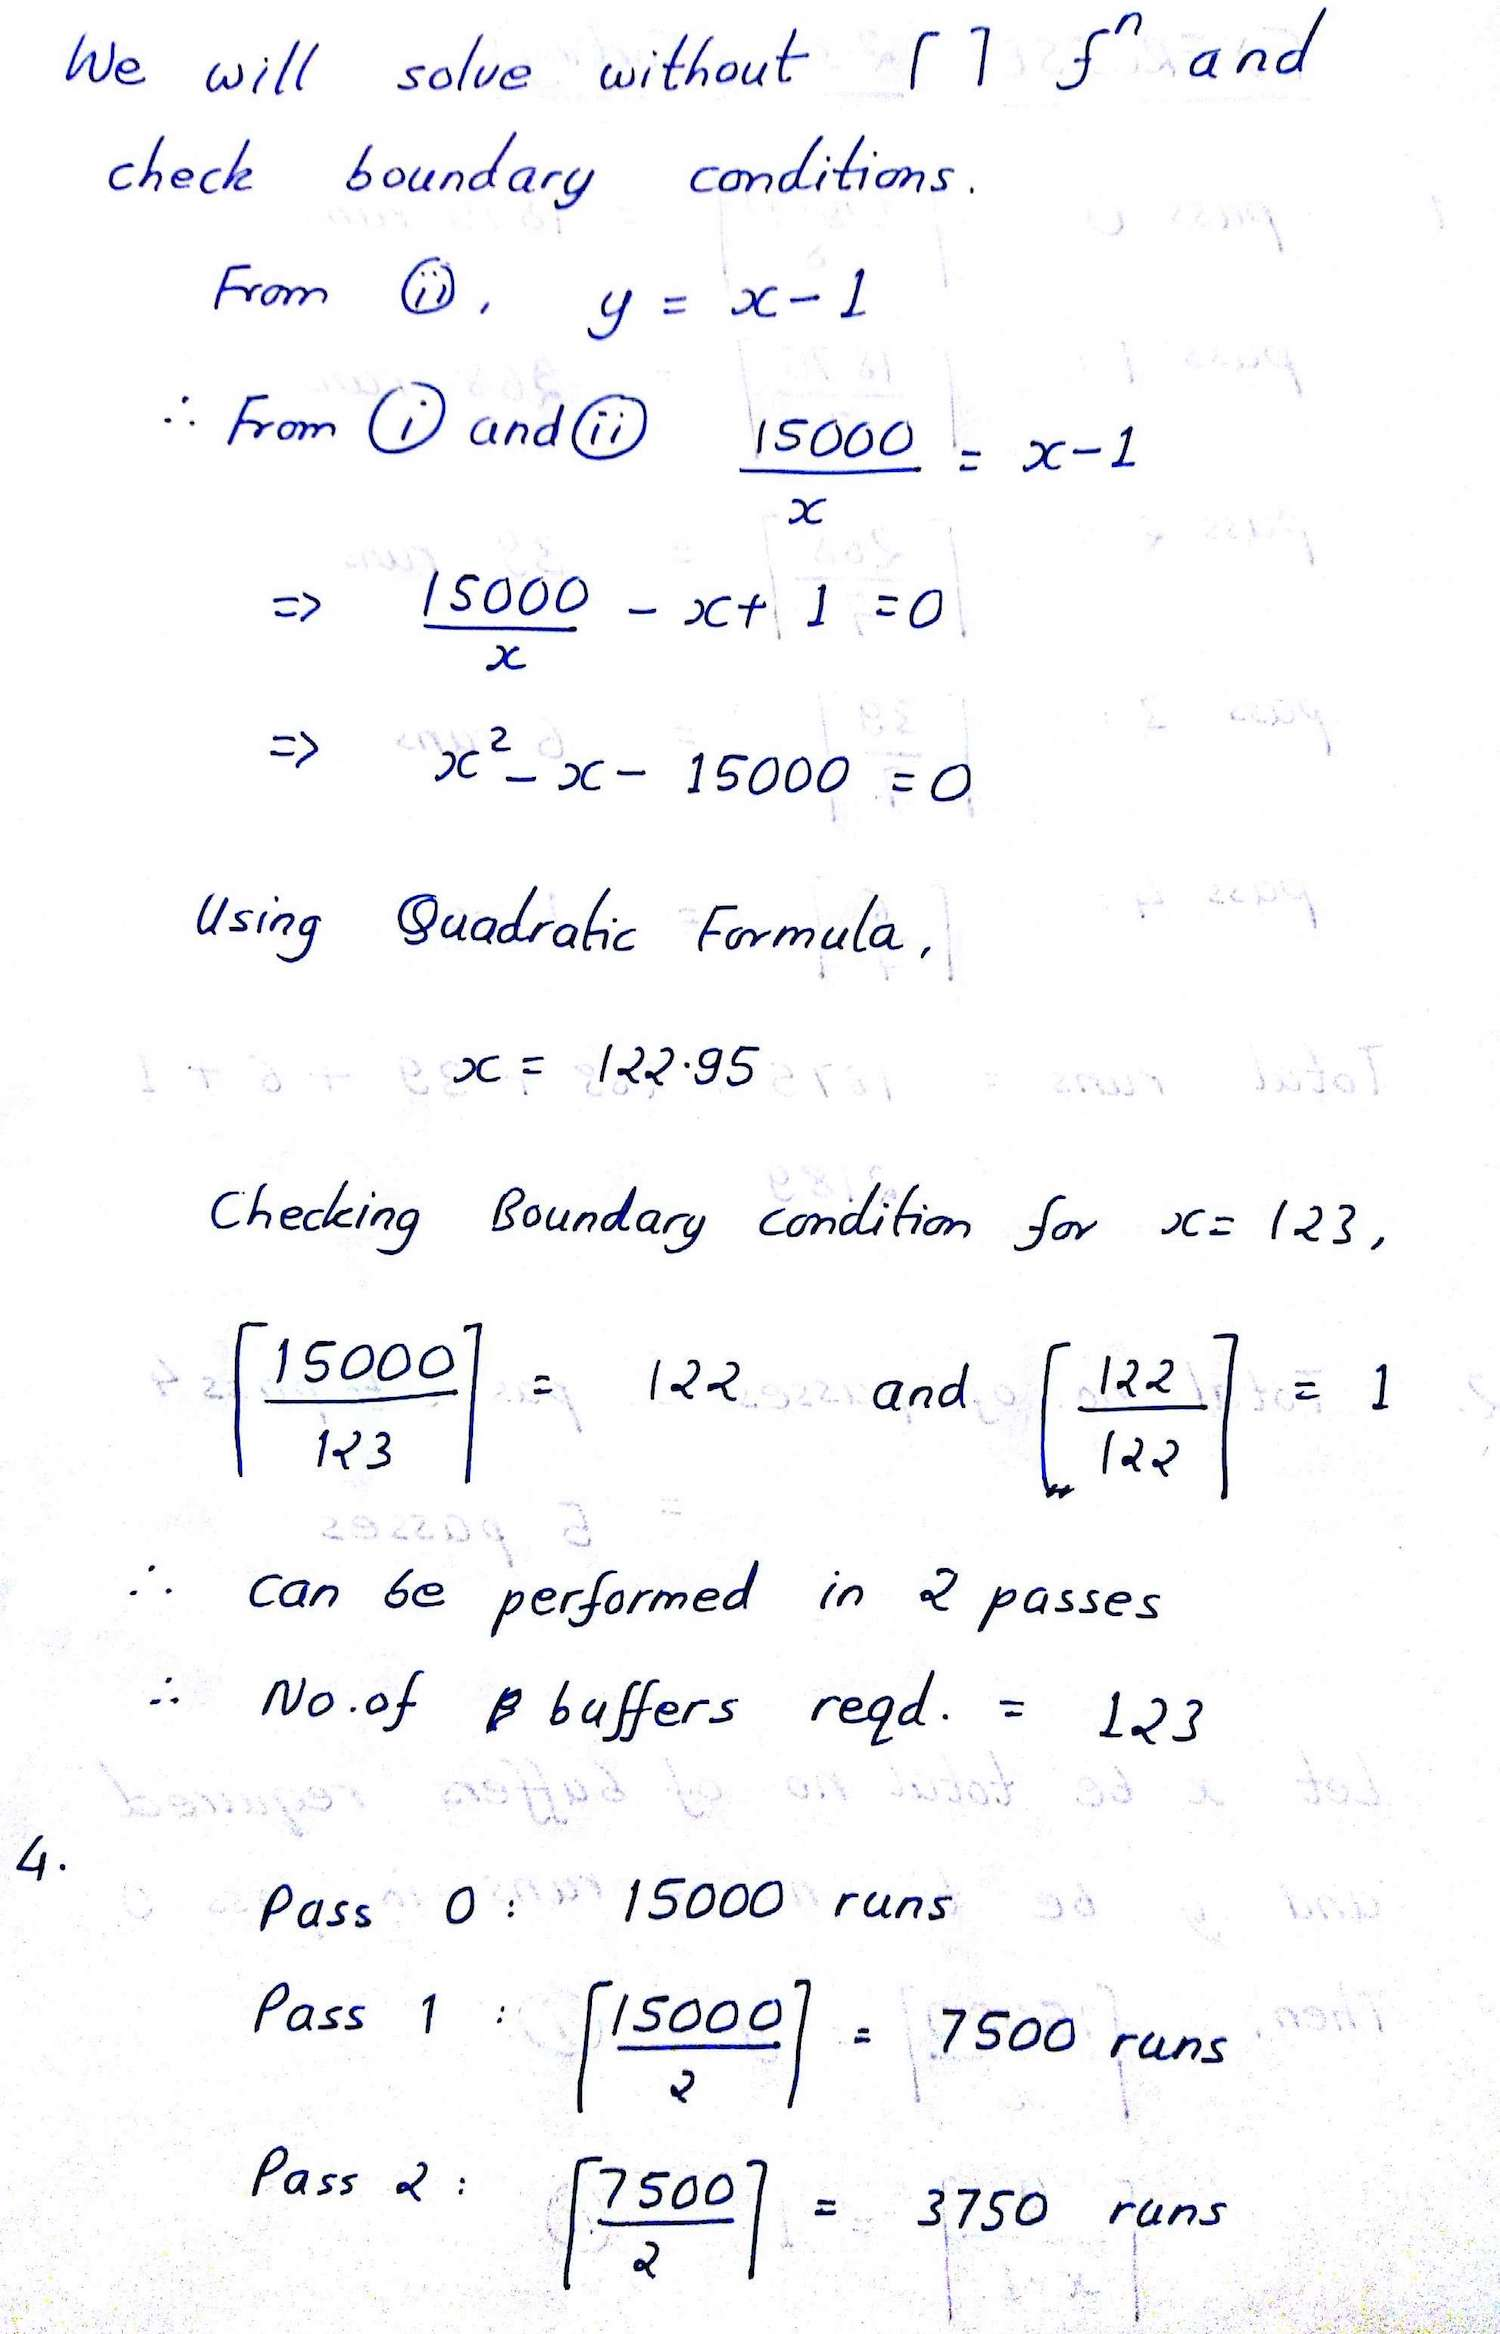
\includegraphics[width=12cm]{images/sol32.jpg}
\caption{Paper-based Solution for Question 3-2}
\end{figure} 

\begin{figure}[h]
\centering
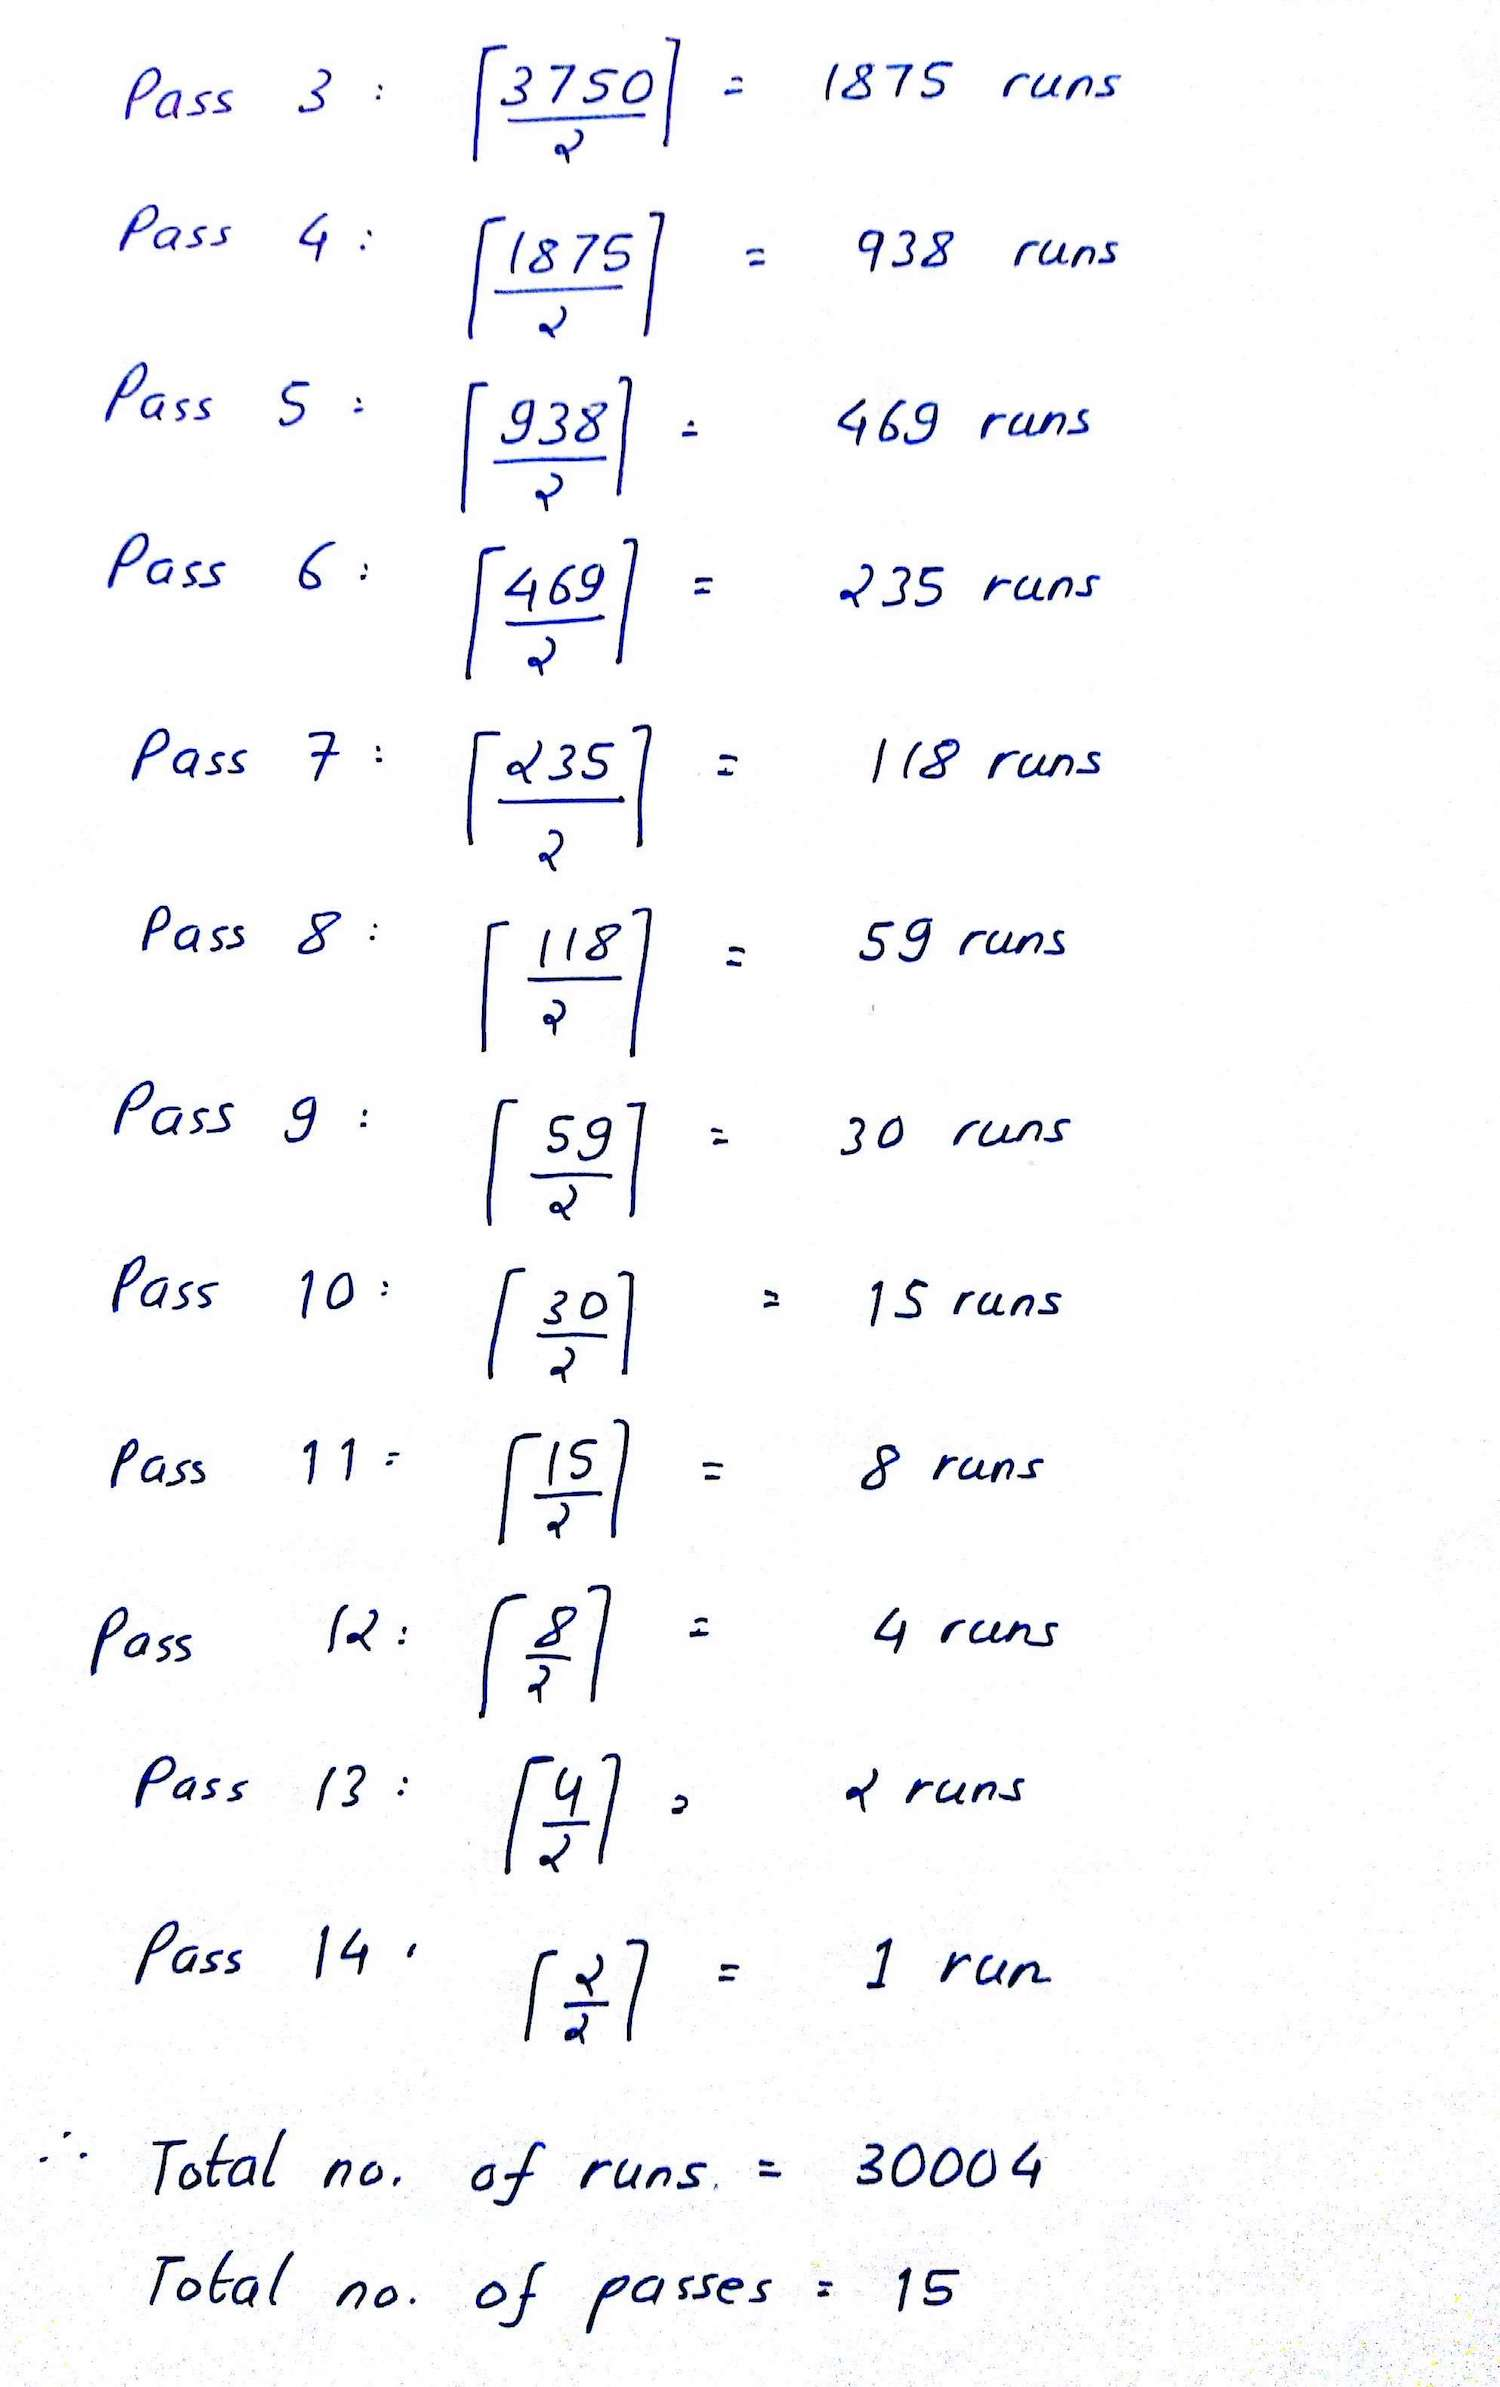
\includegraphics[width=12cm]{images/sol33.jpg}
\caption{Paper-based Solution for Question 3-3}
\end{figure} 

\end{homeworkProblem}

\begin{homeworkProblem}

\textbf{Part 1} \\
Calculate the I/O requirements of a simple nested loop join
 
 \vspace{0.1in} 
     \solution \\ \\ 
     %SOLUTION 
     In the expression below, M and N are the number of pages in the relations Album and Track respectively, $p_M$ and $p_N$ are the number of tuples in each page of the relations. \\
     
     \textbf{M as outer and N as inner relation} \\
     \textbf{Tuple-by-Tuple Simple Nested Loop Join} \\
     $M +  p_M \times M \times N$ \\
     $= 10000 + 100 \times 10000 \times 200000$ \\
     $ = 200000010000 $
          
    \vspace{0.1in}
     \textbf{Page-by-Page Simple Nested Loop Join} \\
     $M + M \times N$ \\
     $= 10000 + 10000 \times 200000$ \\
     $ = 2000010000 $
     
      \vspace{0.1in}
     \textbf{N as outer and M as inner relation} \\
     \textbf{Tuple-by-Tuple Simple Nested Loop Join} \\
     $N +  p_N \times N \times M$ \\
     $= 200000 + 80 \times 200000 \times 10000$ \\
     $ = 160000200000 $
          
    \vspace{0.1in}
     \textbf{Page-by-Page Simple Nested Loop Join} \\
     $M + M \times N$ \\
     $= 200000 + 200000 \times 10000$ \\
     $ = 2000200000 $
     \vspace{0.1in}
     
 \textbf{Part 2} \\
Calculate the I/O requirements of a block nested loop join
 
\vspace{0.1in} 
     \solution \\ \\ 
     %SOLUTION
     Block nested join for 16 buffers: \\
     
      \textbf{M as outer and N as inner relation} \\
     $ 10000 + \lceil \frac{10000}{14} \rceil \times 200000$
     $ = 143010000 $   
     \vspace{0.1in}
     
      \textbf{N as outer and M as inner relation} \\
      $ 200000 + \lceil \frac{200000}{14} \rceil \times 10000$
     $ = 143060000 $   
     \vspace{0.1in}
     
 \textbf{Part 3} \\
Explain the differences between the two algorithms. What are the similarities and differences? How does the block nested loop join reduce I/O costs?
 
 \vspace{0.1in} 
     \solution \\ \\ 
     %SOLUTION
     Tuple-at-a-time Simple Nested Loop Join scans outer relation and then for each tuple, it scans the entire inner relation. On the other hand, the page-at-a-time Simple Nested Loop Join will load the outer relation page-by-page, and then the inner relation for each page. The Block Nested Loop Join, on the other hand, scans entire inner relation for each block of pages in the outer relation. Therefore, the I/O cost of Block Nested Loop Join is lower than cost of both the Simple Nested Loop Joins. 
Moreover, the other important difference is number of buffer pages used in the algorithms. Both tuple-at-a-time nested loop and page-at-time nested loop join use 3 buffer pages to perform the join operation. 1 page as input buffer to scan outer relation,1 page as input buffer to scan inner relation  and 1 page as output buffer. Totally, 3 pages are needed for simple nested loop join. However, block nested loop join uses 1 page as input buffer to scan inner relation S and 1 page as output buffer. The other remaining buffer pages are used to load the blocks of the outer relation R. In this case, 1 buffer page is used as input buffer to scan inner relation  and 1 page as output buffer. Remaining 14 buffer pages are used to block outer relation . As seen, block nested loop join uses entire available buffer pages in the algorithm that means more efficient usage of buffer pages and causing performance increases and decreasing I/O cost. 

The similarities can be indicated as outer-inner relation usage, buffer usage and loop operations in the algorithms. 

     \vspace{0.1in}
     
\end{homeworkProblem}
     
\begin{homeworkProblem}
Given is a relation with 50.000 records. Each page for a node in a B+ tree can hold 20 pointers
to records or pages. A data page can store 20 records. \\

 \textbf{Part 1} \\
Assume that each node is 70 \% full. What is the height of the B+-tree? 

 \vspace{0.1in} 
     \solution \\ \\ 
     %SOLUTION  
     Given that the B+Tree can hold 20 pointers to pages. However, the B+ Tree has 70\% occupancy. Therefore, number of effective pointers to pages that the tree can hold,
     \begin{center} $ \implies 0.7 \times 20 = 14$ \end{center} 
Our B+ Tree can now be represented as Table 1

\begin{table}[]
\centering
\begin{tabular}{|l|l|l|l|}
\hline
Level    & Node & Entries & No. of Pointers \\ \hline
0 (Root) & 1    & 13      & 14              \\ \hline
1        & 14   & 182     & 196             \\ \hline
2        & 196  & 2548    & 2744         \\ \hline  
\end{tabular}
\caption{Different Levels of the B+ Tree}
\label{B+ Tree}
\end{table}

We have 2744 addresses in Level 2 already, which is more than 2500 pointers to pages required in the relations. \\
Therefore, the B-Tree has a depth of \textbf{3}.
Our B+ Tree has a depth of \textbf{3}
 \vspace{0.1in}
     
 \textbf{Part 2} \\
What are the I/O costs for an equality selection on a non-key attribute for the following
cases?

\begin{enumerate}[label = (\alph*)]
\item with a clustered B+-tree of height 3 (matching records are located in one page);
 
 \vspace{0.1in} 
     \solution \\ \\ 
     %SOLUTION
     The clustered index will guide the search, and after the end of the B+ tree traversal, we will need to input the correct page which contains our desired result. Therefore, total I/O is for the tree traversal and retrieving the correct page, i.e. 3 I/Os + 1 I/O = 4.
     Hence, total number of I/Os = \textbf{4} I/Os
     \vspace{0.1in}
     
\item without any index, nor is the file sorted on the attribute occurring in selection;

\vspace{0.1in} 
     \solution \\ \\ 
     %SOLUTION 
     Total number of pages at the leaf node = 2500
    If we consider that all pages need to be scanned, then the I/O costs will be \textbf{2500} I/Os. \\
    However, assuming, on an average that half the total number of pages need to be searched to find the equality results, it gives a total of 1250 I/Os.
          
     \vspace{0.1in}
     
\item with an unclustered B+-tree index of height 4, and there are 2 matching records;

\vspace{0.1in} 
     \solution \\ \\ 
     4 I/Os to traverse the tree + 2 I/Os to retrieve the matching records = \textbf{6} I/Os 
     \vspace{0.1in}

\item with an unclustered B+-tree of height 5 and three tenth of the records match the
selection.

\vspace{0.1in} 
\solution \\ \\ 
     %SOLUTION
     No. of matching records = $\frac{3}{10} \times 50000 = 15000$ records \\
     In the worst case, we need to do 15000 page I/Os, one for each record. Plus the I/Os for traversing the tree. Therefore, a total of 15000 I/Os + 5 I/Os = \textbf{15005} I/Os.   
     \vspace{0.1in}

\end{enumerate}
\end{homeworkProblem}

\end{document}
\documentclass[12pt]{article}

\usepackage{fancyhdr}
\usepackage{extramarks}
\usepackage{amsmath}
\usepackage{amsthm}
\usepackage{amsfonts}
\usepackage{tikz}
\usepackage[plain]{algorithm}
\usepackage{algpseudocode}
\usepackage[export]{adjustbox}
\usepackage[latin1]{inputenc}           %For German characters
\usepackage{enumitem}               %For changing enumeration character
\usepackage{listings}               %For code
\usepackage{csquotes}
\usepackage{graphicx}               %For graphics e.g, images

\usetikzlibrary{automata,positioning}

%
% Basic Document Settings
%

\topmargin=-0.45in
\evensidemargin=0in
\oddsidemargin=0in
\textwidth=6.5in
\textheight=9.0in
\headsep=0.25in

\linespread{1.1}

\pagestyle{fancy}
\lhead{\hmwkAuthorName}
\chead{\hmwkClass\ : \hmwkTitle}
\rhead{\firstxmark}
\lfoot{\lastxmark}
\cfoot{\thepage}

\renewcommand\headrulewidth{0.4pt}
\renewcommand\footrulewidth{0.4pt}

\setlength\parindent{0pt}

%
% Create Problem Sections
%

\newcommand{\enterProblemHeader}[1]{
    \nobreak\extramarks{}{Problem \arabic{#1} continued on next page\ldots}\nobreak{}
    \nobreak\extramarks{Problem \arabic{#1} (continued)}{Problem \arabic{#1} continued on next page\ldots}\nobreak{}
}

\newcommand{\exitProblemHeader}[1]{
    \nobreak\extramarks{Problem \arabic{#1} (continued)}{Problem \arabic{#1} continued on next page\ldots}\nobreak{}
    \stepcounter{#1}
    \nobreak\extramarks{Problem \arabic{#1}}{}\nobreak{}
}

\setcounter{secnumdepth}{0}
\newcounter{partCounter}
\newcounter{homeworkProblemCounter}
\setcounter{homeworkProblemCounter}{1}
\nobreak\extramarks{Problem \arabic{homeworkProblemCounter}}{}\nobreak{}

%
% Homework Problem Environment
%
% This environment takes an optional argument. When given, it will adjust the
% problem counter. This is useful for when the problems given for your
% assignment aren't sequential. See the last 3 problems of this template for an
% example.
%
\newenvironment{homeworkProblem}[1][-1]{
    \ifnum#1>0
        \setcounter{homeworkProblemCounter}{#1}
    \fi
    \section{Problem \arabic{homeworkProblemCounter}}
    \setcounter{partCounter}{1}
    \enterProblemHeader{homeworkProblemCounter}
}{
    \exitProblemHeader{homeworkProblemCounter}
}

%
% Homework Details
%   - Title
%   - Due date
%   - Class
%   - Section/Time
%   - Instructor
%   - Author
%

\newcommand{\hmwkTitle}{Assignment\ \#2}
\newcommand{\hmwkDueDate}{November 15, 2016}
\newcommand{\hmwkClass}{Implementation of Databases}
\newcommand{\hmwkAuthorName}{Sanchit Alekh}
\newcommand{\hmwkClassTime}{MSc. Software Systems Engineering}
\newcommand{\hmwkClassInstructor}{Universitätsprofessor Dr. rer. pol. Matthias Jarke}
\newcommand{\hmwkClassInstructors}{Dr. rer. nat. Christoph Quix}

%
% Title Page
%



\title{
   \begin{center}
   \vspace*{-20mm}
   
\includegraphics[width=0.4\textwidth, right]{images/rwth_logo.png}
   \\
   \vspace*{3cm}
    \textmd{\textbf{\hmwkClass}}\\
    \textmd{\textbf{\hmwkTitle}}\\
    \normalsize\vspace{0.1in}\small{Due\ on\ \hmwkDueDate } \\
    \vspace{0.1in}\large{\textit{\hmwkClassInstructor}} \\
    \vspace{0.1in}\large{\textit{\hmwkClassInstructors}} \\
    \vspace{3in}
     \textbf{Submitted by:} \\
     \vspace{0.25in}
    \large{Sanchit Alekh, Idil Esen Zülfikar, Nihal Hegde} \\
    %\author{\textbf{\hmwkAuthorName}}
    \vspace{0.1in} \large{\textit{\hmwkClassTime}} \\
    %\vspace{0.1in} \large{\textit{Matrikelnummer : 359831}}
    \end{center}
    }


\date{}

\renewcommand{\part}[1]{\textbf{\large Part \Alph{partCounter}}\stepcounter{partCounter}\\}

%
% Various Helper Commands
%

% Useful for algorithms
\newcommand{\alg}[1]{\textsc{\bfseries \footnotesize #1}}

% For derivatives
\newcommand{\deriv}[1]{\frac{\mathrm{d}}{\mathrm{d}x} (#1)}

% For partial derivatives
\newcommand{\pderiv}[2]{\frac{\partial}{\partial #1} (#2)}

% Integral dx
\newcommand{\dx}{\mathrm{d}x}

% Alias for the Solution section header
\newcommand{\solution}{\textbf{\large Solution}}

% Probability commands: Expectation, Variance, Covariance, Bias
\newcommand{\E}{\mathrm{E}}
\newcommand{\Var}{\mathrm{Var}}
\newcommand{\Cov}{\mathrm{Cov}}
\newcommand{\Bias}{\mathrm{Bias}}

\begin{document}

\maketitle

\pagebreak

\begin{homeworkProblem}
    
    \textbf{Part 1} \\
    Variants of relational algebra are used internally in DBMS to represent queries and query evaluation plans. Please explain, why relational algebra is suitable for this?
    
    \vspace{0.1in}
    \solution \\
    One of the most desirable properties of Relational Algebra is that queries are composed using a collection of operators, and every operator accepts one or two relation instances as arguments and returns a relation instance as the result. This property makes extremely easy and efficient to compose operators to form a complex query. A relational algebra expression can be recursively defined to be a relation, a unary algebra operator applied to a single expression, or a binary algebra operator applied to two expressions. 
This procedural nature of relational algebra is the main reason why it is used internally in DBMS to represent queries and evaluation plans. The approach allows us to think of an algebra expression as an imperative execution plan for a declarative SQL query. It can be used for evaluating a query, and relational systems in fact use algebra expressions to represent query evaluation plans.
        
    \vspace{0.1in}
    
    \textbf{Part 2} \\
    What does \enquote{relational completeness} mean (in your own words, please)? Show that SQL is
relationally complete by enumerating SQL constructs corresponding to selection, projection,
cartesian product, union, and difference.
    
    \vspace{0.1in}
    \solution \\
    \enquote{Relational Completeness} of a query methodology means that each and every query that can be expressed using that methodology, can also be expressed as a relational algebra query. In this case, SQL is referred to as \enquote*{Relationally Complete} because every legal construct in SQL can be expressed as a Relational Algebra query.
        
These are the examples of Relational Algebra expressions and their equivalent expressions in SQL. The following examples are derived from the \textit{Mondial} database.

\begin{itemize}

\item \textbf{SELECTION} \\
Relational Algebra: $ \sigma_{Area > 650} (Island)$ \\
SQL:  \textit{Select * From Island Where Area $>$ 650;}

\item \textbf{PROJECTION} \\
Relational Algebra: $ \pi_{Name, Islands, Area, Height} (Island)$ \\
SQL: \textit{Select Name, Islands, Area, Height From Island;}

\item \textbf{CARTESIAN PRODUCT} \\
Relational Algebra:  $ Island \times islandIn$ \\
SQL: \textit{Select * From Island CROSS JOIN islandIn;}

\item \textbf{UNION} \\
Relational Algebra:  $ \pi_{name} (Desert) \cup \pi_{name} (geo\_Desert)$ \\
SQL: \textit{Select name From Desert or Select name From geo\_Desert}

\item \textbf{SET DIFFERENCE} \\
Relational Algebra: $ \pi_{name} (\sigma_{height > 5000} (Mountain)) - \pi_{name}( \sigma_{type > 'volcanic')} (Mountain) $ \\
SQL: \textit{Select name From Mountain where height $>$ 5000 MINUS Select name From Mountain where type='volcanic'}
\end{itemize}
        
    \vspace{0.1in}
        
     \textbf{Part 3} \\
    Explain how the intersection operator is used in relational algebra. What is important for
its usage? Is it omittable (i.e., could you express it by other operators)? If so, please give
the corresponding relational algebra.
    
    \vspace{0.1in}
    \solution \\
    The \enquote*{Intersection} operator is represented in Relational Algebra with the help of the $\cap$ symbol. Although it is not a fundamental set-operator, it is an extremely widely used operation, and it is helpful to define it separately. An example use of the intersection operator is as follows:
    
    \begin{center} $ \pi_{name} (Desert) \cap \pi_{name} (geo\_Desert) $ \end{center}
    
The important condition for using the \textit{Intersection} operator is that the two sets which have to be intersected must be \textit{union-compatible}. This follows from the fact that intersection is defined in terms of set difference.

Yes, Intersection is not a fundamental set-operator, and it can be expressed in terms of the set-difference operator. Therefore, it is omittable. A general expression for the intersection operator in terms of the set-difference operator is:

    \begin{center} $ A \cup B \leftrightarrow A \setminus ( A \setminus B) $ \end{center}
    
Therefore, the example Relational Algebra query illustrated above can be represented by the equivalent query without the use of set-intersection as follows:

    \begin{center} $ \pi_{name} (Desert) - (\pi_{name} (Desert) - \pi_{name} (geo\_Desert))$ \end{center}
    
\begin{figure}[h]
\centering
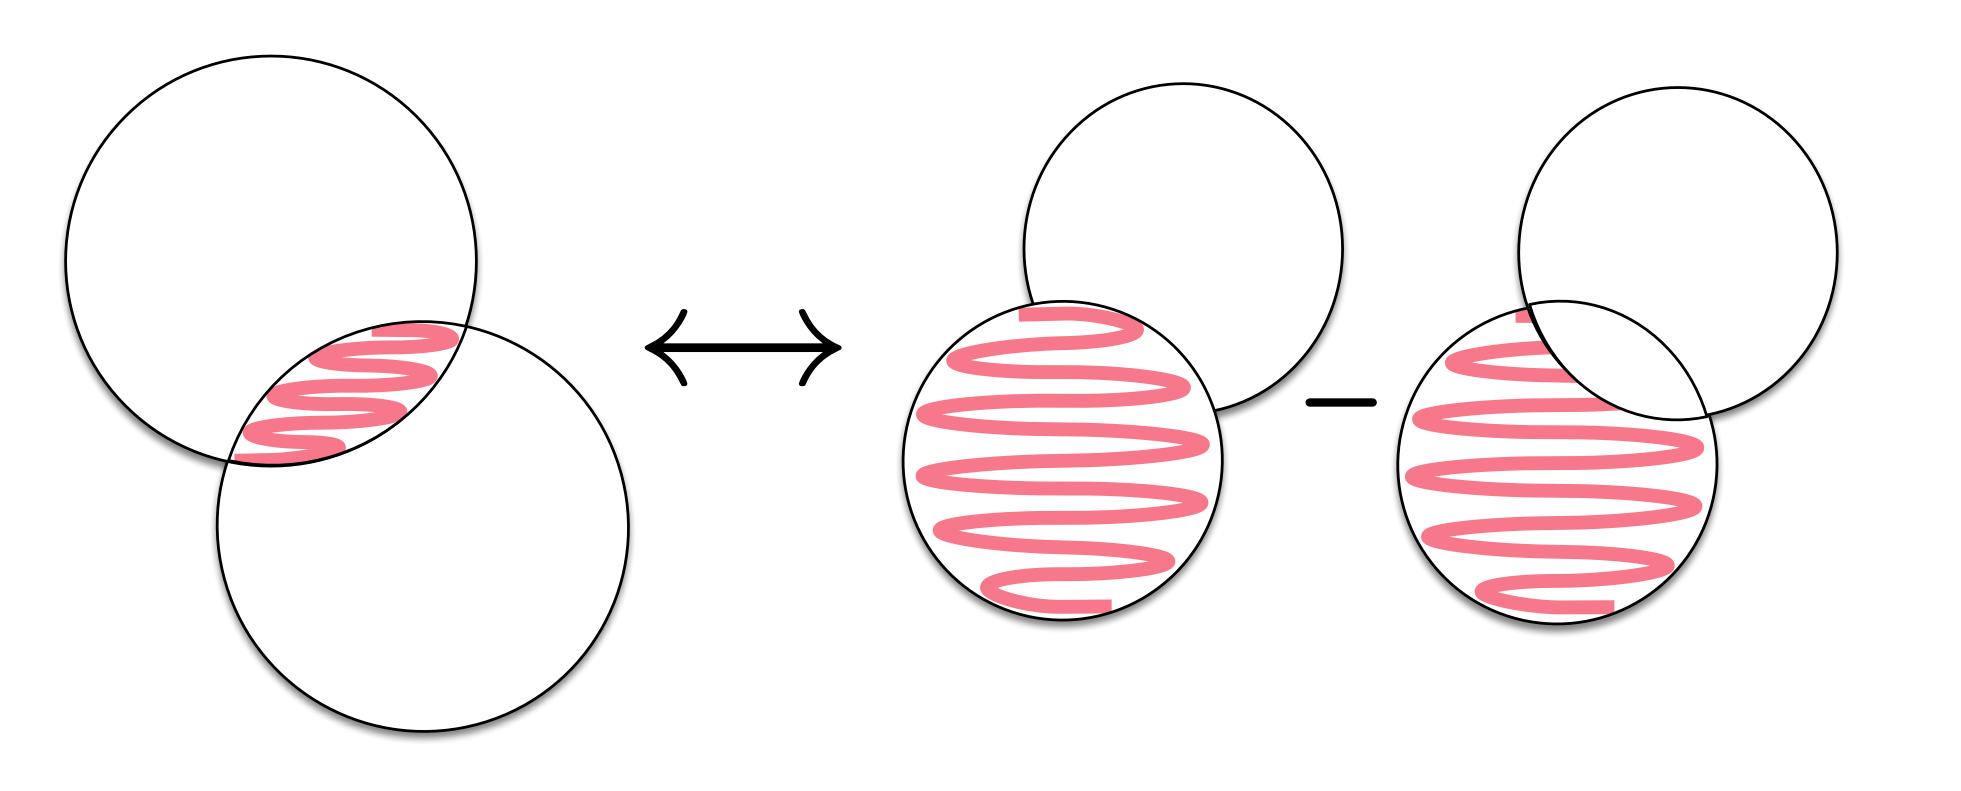
\includegraphics[width=12cm]{images/intersection1.png}
\caption{Venn-Diagram showing the definition of Intersection in terms of Set Difference}
\end{figure}
        
    \vspace{0.1in}
    
     \textbf{Part 4} \\
    Explain the difference between DRC and TRC.
    
    \vspace{0.1in}
        \solution \\
In Tuple Relational Calculus (TRC), the variables typically range over tuples, i.e. they directly represent tuples. On the other hand, in Domain Relational Calculus (DRC), the variables range over domain elements, i.e. field values. In TRC, tuples are semantically equivalent to variables, i.e. field referencing can be used to select tuple parts. On the other hand, in DRC, formal variables are explicit and have to be defined.
    \vspace{0.1in}
    
    
\end{homeworkProblem}   

\begin{homeworkProblem}

\textbf{Part 1} \\

The names of the seas that are deeper than 3000 mt and into which at least one river finally flows.

\vspace{0.1in}
    \solution \\
      
    $<name> \mid \exists depth, rname, river, lake, sea, length, sLong, sLat, mount, sAlt, estLong, estLat \\
    Sea(name, depth) \wedge  \\ River(rname, river, lake, sea, length, sLong, sLat, mount, sAlt, estLong, estLat) \wedge \\ depth > 3000 \wedge sea = name$ 
    \vspace{0.1in}
    
\textbf{Part 2} \\
The names of the groups of islands that consist only of islands that are neither 'volcanic' nor
'coral'.

 \vspace{0.1in}
    \solution \\ \\    
   %SOLUTION
   $<islands> \mid \exists name, area, height, type, long, lat \\
Island(name, islands, area, height, type, long, lat) \wedge \\
type \notin \{volcanic, coral\} \wedge islands \neq \emptyset  $
    \vspace{0.1in}    

\textbf{Part 3} \\
The name of the mountain, the name of the mountains where it belongs to and the name of
the country where the mountain is located for each mountain that is located on an island
that is of type 'coral'.

 
 \vspace{0.1in} 
     \solution \\ \\ 
     %SOLUTION   
     $<moiMountain, mMountains, gmCountry> \mid \exists \\ moiIsland, mHeight, mType, mLong, mLat, \\ iIslands, iArea, iHeight, iType, iLong, iLat, gmProvince \\
mountainOnIsland(moiMountain, moiIsland) \wedge \\ Mountain(moiMountain, mMountains, mHeight, mType, mLong, mLat) \wedge \\ geo\_Mountain(moiMountain, gmCountry, gmProvince)  \wedge \\
Island(moiIsland, iIslands, iArea, iHeight, iType, iLong, iLat) \wedge iType \neq "coral" $

     \vspace{0.1in}

    
\textbf{Part 4} \\
Give the name and country name of all cities with a population higher than 500,000.

 \vspace{0.1in} 
     \solution \\ \\    
    %SOLUTION
   $<cName, coName> \mid \exists cCountry, cProvince, cPopulation, cLong, cLat, \\
   coCapital, coProvince, coArea, coPopulation \\
City(cName, cCountry, cProvince, cPopulation, cLong, cLat)  \wedge \\
Country(cCountry, coName, coCapital, coProvince, coArea, coPopulation) \wedge \\
cPopulation > 500000 $
 
    \vspace{0.1in}
        
\end{homeworkProblem}

\begin{homeworkProblem}
Suppose you have a file of 15,000 pages and eight buffer pages and you are sorting it using general
(external) merge-sort. Please answer the following questions: \\

\textbf{Part 1} \\
How many runs will you produce? Remark: When a file is sorted, in intermediate steps
subfiles are created. Each sorted subfile is called a run. See also slide 35 in Chapter 2.
 \textbf{Note: Detailed solution of Q3 is produced in \textit{Figures 2, 3 and 4.}}
 
 \vspace{0.1in} 
     \solution \\
     %SOLUTION
     \textbf{2189} runs will be produced   
     \vspace{0.1in}
     
 \textbf{Part 2} \\
How many passes will it take to sort the file completely?
 
 \vspace{0.1in} 
     \solution \\ 
    It will take \textbf{5} passes   
     \vspace{0.1in}
     
 \textbf{Part 3} \\
How many buffer pages do you need at least to sort the file in two passes? 

 \vspace{0.1in} 
     \solution \\
     With \textbf{123} buffers, you can sort the file in two passes 
     \vspace{0.1in}
 
 \textbf{Part 4} \\
How many runs and passes would a Two-Way-Sort algorithm take?
 
 \vspace{0.1in} 
     \solution \\
     %SOLUTION
     Two-Way Sort Algorithm will take \textbf{30004} runs and \textbf{15} passes   
     \vspace{0.1in}   
     
\begin{figure}[h]
\centering
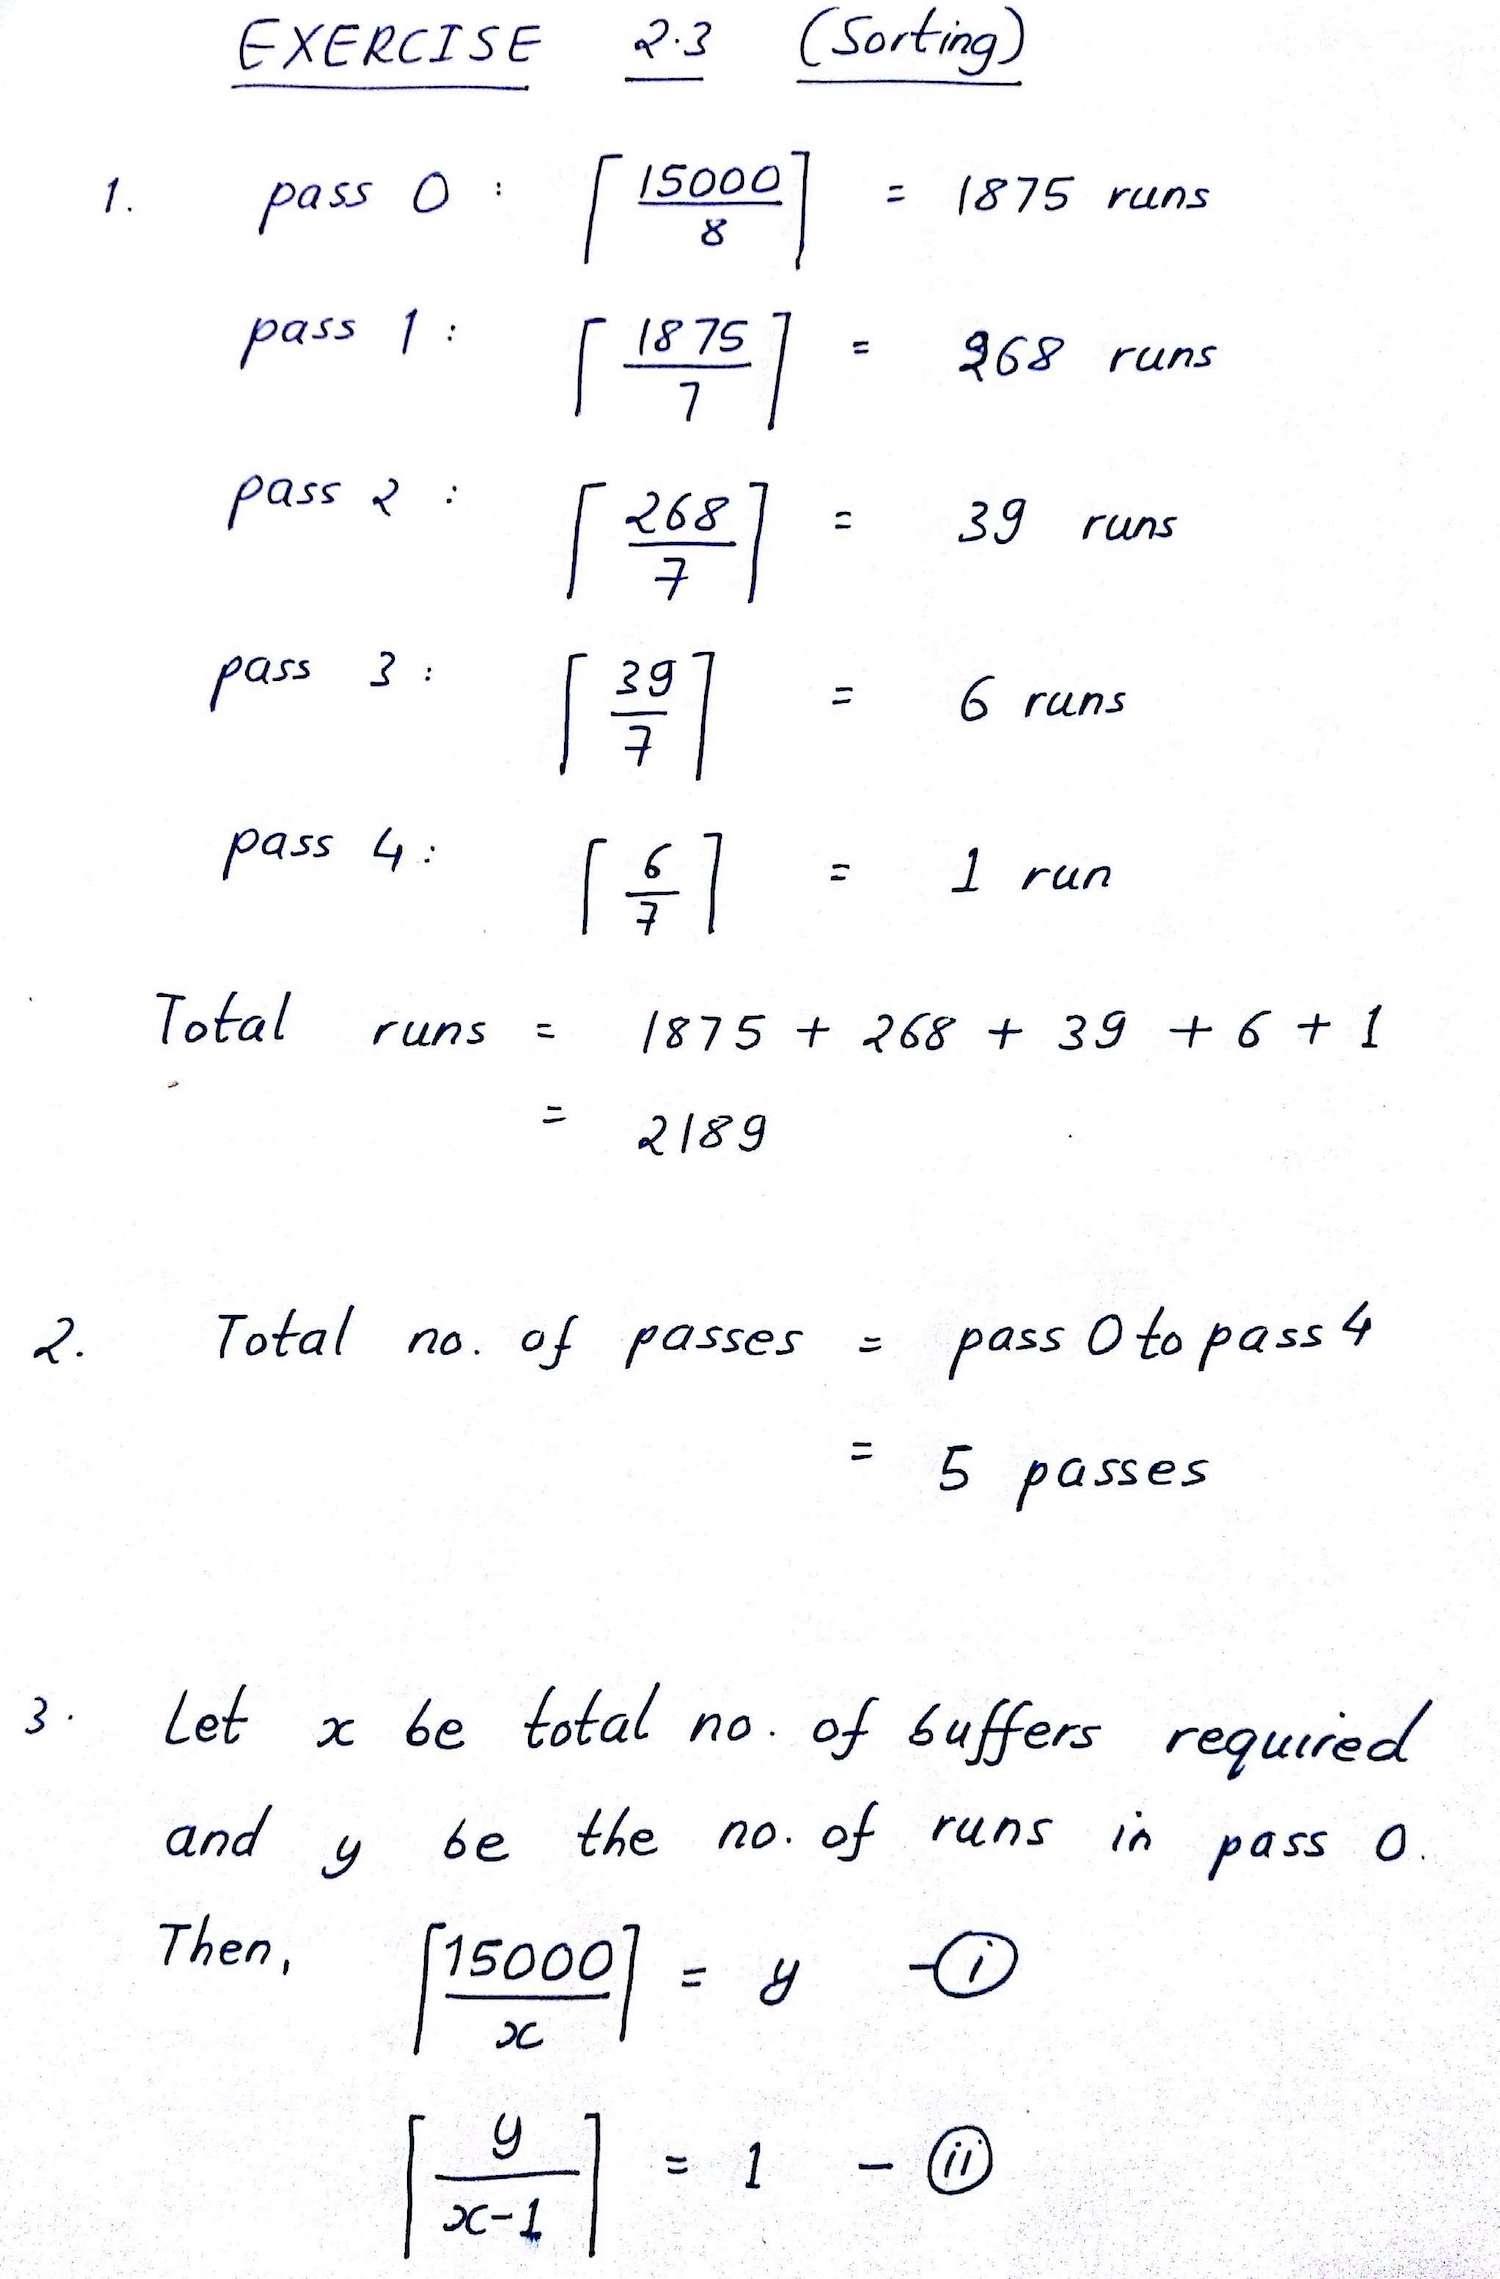
\includegraphics[width=12cm]{images/sol31.jpg}
\caption{Paper-based Solution for Question 3-1}
\end{figure} 

\begin{figure}[h]
\centering
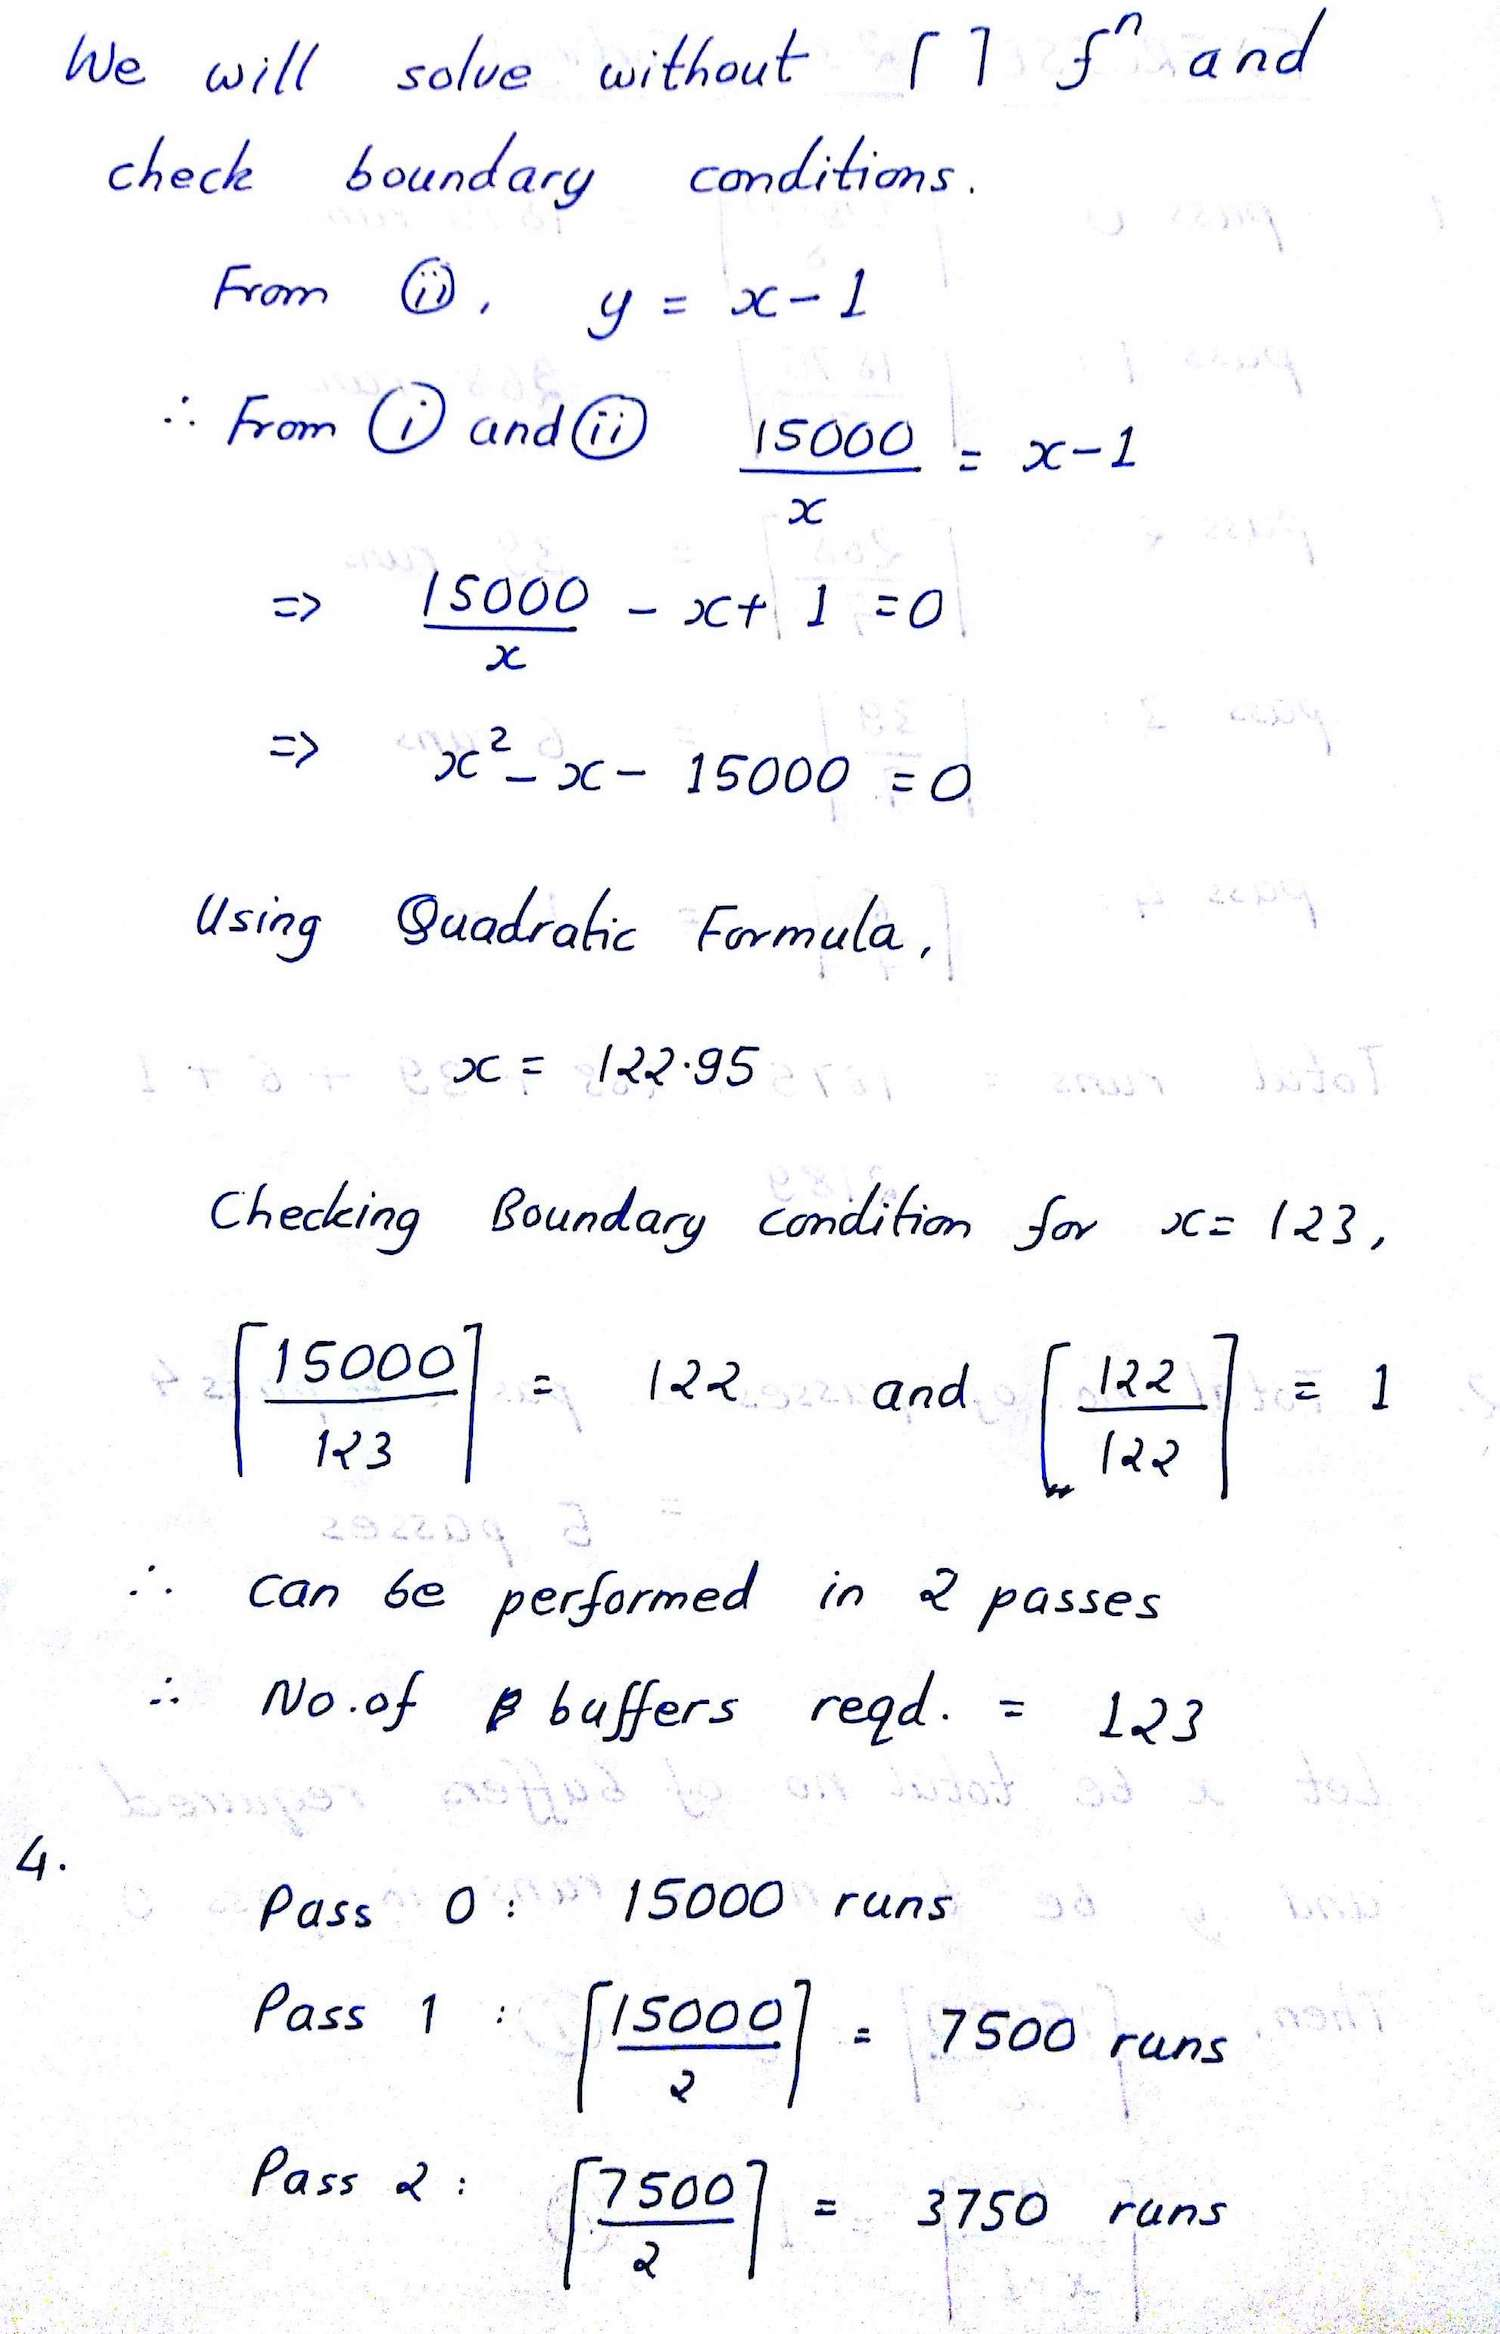
\includegraphics[width=12cm]{images/sol32.jpg}
\caption{Paper-based Solution for Question 3-2}
\end{figure} 

\begin{figure}[h]
\centering
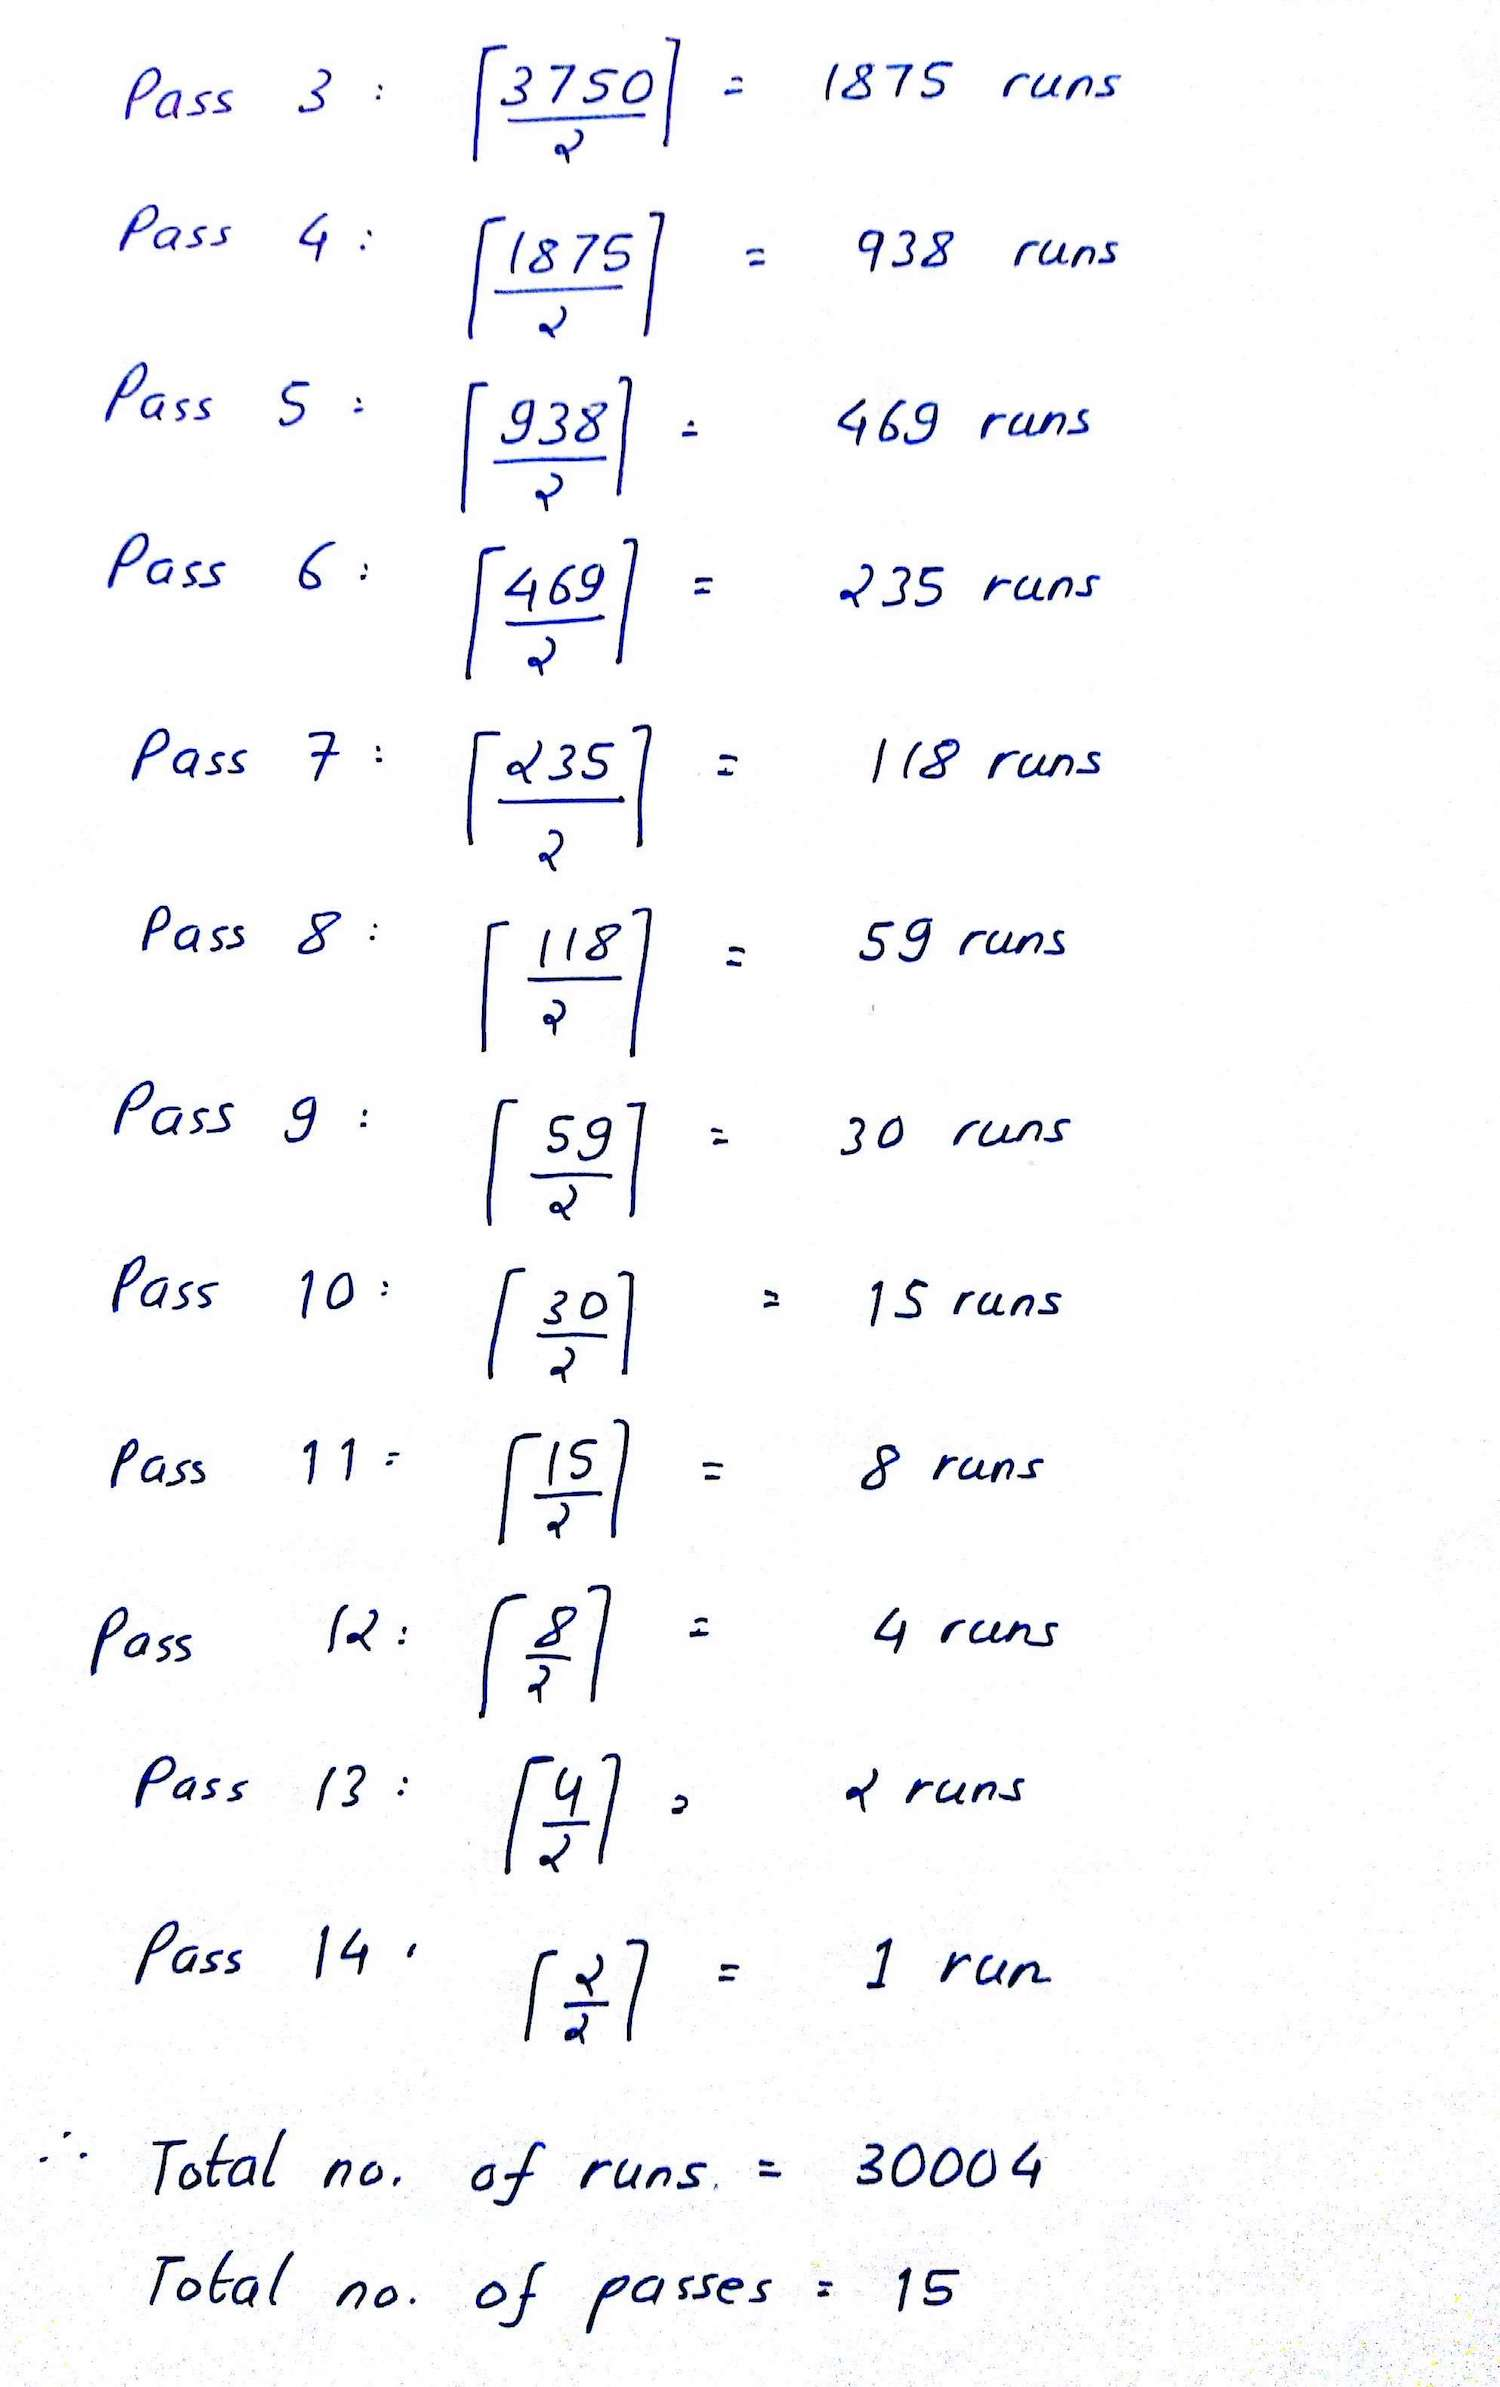
\includegraphics[width=12cm]{images/sol33.jpg}
\caption{Paper-based Solution for Question 3-3}
\end{figure} 

\end{homeworkProblem}

\begin{homeworkProblem}

\textbf{Part 1} \\
Calculate the I/O requirements of a simple nested loop join
 
 \vspace{0.1in} 
     \solution \\ \\ 
     %SOLUTION 
     In the expression below, M and N are the number of pages in the relations Album and Track respectively, $p_M$ and $p_N$ are the number of tuples in each page of the relations. \\
     
     \textbf{M as outer and N as inner relation} \\
     \textbf{Tuple-by-Tuple Simple Nested Loop Join} \\
     $M +  p_M \times M \times N$ \\
     $= 10000 + 100 \times 10000 \times 200000$ \\
     $ = 200000010000 $
          
    \vspace{0.1in}
     \textbf{Page-by-Page Simple Nested Loop Join} \\
     $M + M \times N$ \\
     $= 10000 + 10000 \times 200000$ \\
     $ = 2000010000 $
     
      \vspace{0.1in}
     \textbf{N as outer and M as inner relation} \\
     \textbf{Tuple-by-Tuple Simple Nested Loop Join} \\
     $N +  p_N \times N \times M$ \\
     $= 200000 + 80 \times 200000 \times 10000$ \\
     $ = 160000200000 $
          
    \vspace{0.1in}
     \textbf{Page-by-Page Simple Nested Loop Join} \\
     $M + M \times N$ \\
     $= 200000 + 200000 \times 10000$ \\
     $ = 2000200000 $
     \vspace{0.1in}
     
 \textbf{Part 2} \\
Calculate the I/O requirements of a block nested loop join
 
\vspace{0.1in} 
     \solution \\ \\ 
     %SOLUTION
     Block nested join for 16 buffers: \\
     
      \textbf{M as outer and N as inner relation} \\
     $ 10000 + \lceil \frac{10000}{14} \rceil \times 200000$
     $ = 143010000 $   
     \vspace{0.1in}
     
      \textbf{N as outer and M as inner relation} \\
      $ 200000 + \lceil \frac{200000}{14} \rceil \times 10000$
     $ = 143060000 $   
     \vspace{0.1in}
     
 \textbf{Part 3} \\
Explain the differences between the two algorithms. What are the similarities and differences? How does the block nested loop join reduce I/O costs?
 
 \vspace{0.1in} 
     \solution \\ \\ 
     %SOLUTION
     Tuple-at-a-time Simple Nested Loop Join scans outer relation and then for each tuple, it scans the entire inner relation. On the other hand, the page-at-a-time Simple Nested Loop Join will load the outer relation page-by-page, and then the inner relation for each page. The Block Nested Loop Join, on the other hand, scans entire inner relation for each block of pages in the outer relation. Therefore, the I/O cost of Block Nested Loop Join is lower than cost of both the Simple Nested Loop Joins. 
Moreover, the other important difference is number of buffer pages used in the algorithms. Both tuple-at-a-time nested loop and page-at-time nested loop join use 3 buffer pages to perform the join operation. 1 page as input buffer to scan outer relation,1 page as input buffer to scan inner relation  and 1 page as output buffer. Totally, 3 pages are needed for simple nested loop join. However, block nested loop join uses 1 page as input buffer to scan inner relation S and 1 page as output buffer. The other remaining buffer pages are used to load the blocks of the outer relation R. In this case, 1 buffer page is used as input buffer to scan inner relation  and 1 page as output buffer. Remaining 14 buffer pages are used to block outer relation . As seen, block nested loop join uses entire available buffer pages in the algorithm that means more efficient usage of buffer pages and causing performance increases and decreasing I/O cost. 

The similarities can be indicated as outer-inner relation usage, buffer usage and loop operations in the algorithms. 

     \vspace{0.1in}
     
\end{homeworkProblem}
     
\begin{homeworkProblem}
Given is a relation with 50.000 records. Each page for a node in a B+ tree can hold 20 pointers
to records or pages. A data page can store 20 records. \\

 \textbf{Part 1} \\
Assume that each node is 70 \% full. What is the height of the B+-tree? 

 \vspace{0.1in} 
     \solution \\ \\ 
     %SOLUTION  
     Given that the B+Tree can hold 20 pointers to pages. However, the B+ Tree has 70\% occupancy. Therefore, number of effective pointers to pages that the tree can hold,
     \begin{center} $ \implies 0.7 \times 20 = 14$ \end{center} 
Our B+ Tree can now be represented as Table 1

\begin{table}[]
\centering
\begin{tabular}{|l|l|l|l|}
\hline
Level    & Node & Entries & No. of Pointers \\ \hline
0 (Root) & 1    & 13      & 14              \\ \hline
1        & 14   & 182     & 196             \\ \hline
2        & 196  & 2548    & 2744         \\ \hline  
\end{tabular}
\caption{Different Levels of the B+ Tree}
\label{B+ Tree}
\end{table}

We have 2744 addresses in Level 2 already, which is more than 2500 pointers to pages required in the relations. \\
Therefore, the B-Tree has a depth of \textbf{3}.
Our B+ Tree has a depth of \textbf{3}
 \vspace{0.1in}
     
 \textbf{Part 2} \\
What are the I/O costs for an equality selection on a non-key attribute for the following
cases?

\begin{enumerate}[label = (\alph*)]
\item with a clustered B+-tree of height 3 (matching records are located in one page);
 
 \vspace{0.1in} 
     \solution \\ \\ 
     %SOLUTION
     The clustered index will guide the search, and after the end of the B+ tree traversal, we will need to input the correct page which contains our desired result. Therefore, total I/O is for the tree traversal and retrieving the correct page, i.e. 3 I/Os + 1 I/O = 4.
     Hence, total number of I/Os = \textbf{4} I/Os
     \vspace{0.1in}
     
\item without any index, nor is the file sorted on the attribute occurring in selection;

\vspace{0.1in} 
     \solution \\ \\ 
     %SOLUTION 
     Total number of pages at the leaf node = 2500
    If we consider that all pages need to be scanned, then the I/O costs will be \textbf{2500} I/Os. \\
    However, assuming, on an average that half the total number of pages need to be searched to find the equality results, it gives a total of 1250 I/Os.
          
     \vspace{0.1in}
     
\item with an unclustered B+-tree index of height 4, and there are 2 matching records;

\vspace{0.1in} 
     \solution \\ \\ 
     4 I/Os to traverse the tree + 2 I/Os to retrieve the matching records = \textbf{6} I/Os 
     \vspace{0.1in}

\item with an unclustered B+-tree of height 5 and three tenth of the records match the
selection.

\vspace{0.1in} 
\solution \\ \\ 
     %SOLUTION
     No. of matching records = $\frac{3}{10} \times 50000 = 15000$ records \\
     In the worst case, we need to do 15000 page I/Os, one for each record. Plus the I/Os for traversing the tree. Therefore, a total of 15000 I/Os + 5 I/Os = \textbf{15005} I/Os.   
     \vspace{0.1in}

\end{enumerate}
\end{homeworkProblem}

\end{document}
\documentclass[12pt]{article}

\usepackage{fancyhdr}
\usepackage{extramarks}
\usepackage{amsmath}
\usepackage{amsthm}
\usepackage{amsfonts}
\usepackage{tikz}
\usepackage[plain]{algorithm}
\usepackage{algpseudocode}
\usepackage[export]{adjustbox}
\usepackage[latin1]{inputenc}           %For German characters
\usepackage{enumitem}               %For changing enumeration character
\usepackage{listings}               %For code
\usepackage{csquotes}
\usepackage{graphicx}               %For graphics e.g, images

\usetikzlibrary{automata,positioning}

%
% Basic Document Settings
%

\topmargin=-0.45in
\evensidemargin=0in
\oddsidemargin=0in
\textwidth=6.5in
\textheight=9.0in
\headsep=0.25in

\linespread{1.1}

\pagestyle{fancy}
\lhead{\hmwkAuthorName}
\chead{\hmwkClass\ : \hmwkTitle}
\rhead{\firstxmark}
\lfoot{\lastxmark}
\cfoot{\thepage}

\renewcommand\headrulewidth{0.4pt}
\renewcommand\footrulewidth{0.4pt}

\setlength\parindent{0pt}

%
% Create Problem Sections
%

\newcommand{\enterProblemHeader}[1]{
    \nobreak\extramarks{}{Problem \arabic{#1} continued on next page\ldots}\nobreak{}
    \nobreak\extramarks{Problem \arabic{#1} (continued)}{Problem \arabic{#1} continued on next page\ldots}\nobreak{}
}

\newcommand{\exitProblemHeader}[1]{
    \nobreak\extramarks{Problem \arabic{#1} (continued)}{Problem \arabic{#1} continued on next page\ldots}\nobreak{}
    \stepcounter{#1}
    \nobreak\extramarks{Problem \arabic{#1}}{}\nobreak{}
}

\setcounter{secnumdepth}{0}
\newcounter{partCounter}
\newcounter{homeworkProblemCounter}
\setcounter{homeworkProblemCounter}{1}
\nobreak\extramarks{Problem \arabic{homeworkProblemCounter}}{}\nobreak{}

%
% Homework Problem Environment
%
% This environment takes an optional argument. When given, it will adjust the
% problem counter. This is useful for when the problems given for your
% assignment aren't sequential. See the last 3 problems of this template for an
% example.
%
\newenvironment{homeworkProblem}[1][-1]{
    \ifnum#1>0
        \setcounter{homeworkProblemCounter}{#1}
    \fi
    \section{Problem \arabic{homeworkProblemCounter}}
    \setcounter{partCounter}{1}
    \enterProblemHeader{homeworkProblemCounter}
}{
    \exitProblemHeader{homeworkProblemCounter}
}

%
% Homework Details
%   - Title
%   - Due date
%   - Class
%   - Section/Time
%   - Instructor
%   - Author
%

\newcommand{\hmwkTitle}{Assignment\ \#2}
\newcommand{\hmwkDueDate}{November 15, 2016}
\newcommand{\hmwkClass}{Implementation of Databases}
\newcommand{\hmwkAuthorName}{Sanchit Alekh}
\newcommand{\hmwkClassTime}{MSc. Software Systems Engineering}
\newcommand{\hmwkClassInstructor}{Universitätsprofessor Dr. rer. pol. Matthias Jarke}
\newcommand{\hmwkClassInstructors}{Dr. rer. nat. Christoph Quix}

%
% Title Page
%



\title{
   \begin{center}
   \vspace*{-20mm}
   
\includegraphics[width=0.4\textwidth, right]{images/rwth_logo.png}
   \\
   \vspace*{3cm}
    \textmd{\textbf{\hmwkClass}}\\
    \textmd{\textbf{\hmwkTitle}}\\
    \normalsize\vspace{0.1in}\small{Due\ on\ \hmwkDueDate } \\
    \vspace{0.1in}\large{\textit{\hmwkClassInstructor}} \\
    \vspace{0.1in}\large{\textit{\hmwkClassInstructors}} \\
    \vspace{3in}
     \textbf{Submitted by:} \\
     \vspace{0.25in}
    \large{Sanchit Alekh, Idil Esen Zülfikar, Nihal Hegde} \\
    %\author{\textbf{\hmwkAuthorName}}
    \vspace{0.1in} \large{\textit{\hmwkClassTime}} \\
    %\vspace{0.1in} \large{\textit{Matrikelnummer : 359831}}
    \end{center}
    }


\date{}

\renewcommand{\part}[1]{\textbf{\large Part \Alph{partCounter}}\stepcounter{partCounter}\\}

%
% Various Helper Commands
%

% Useful for algorithms
\newcommand{\alg}[1]{\textsc{\bfseries \footnotesize #1}}

% For derivatives
\newcommand{\deriv}[1]{\frac{\mathrm{d}}{\mathrm{d}x} (#1)}

% For partial derivatives
\newcommand{\pderiv}[2]{\frac{\partial}{\partial #1} (#2)}

% Integral dx
\newcommand{\dx}{\mathrm{d}x}

% Alias for the Solution section header
\newcommand{\solution}{\textbf{\large Solution}}

% Probability commands: Expectation, Variance, Covariance, Bias
\newcommand{\E}{\mathrm{E}}
\newcommand{\Var}{\mathrm{Var}}
\newcommand{\Cov}{\mathrm{Cov}}
\newcommand{\Bias}{\mathrm{Bias}}

\begin{document}

\maketitle

\pagebreak

\begin{homeworkProblem}
    
    \textbf{Part 1} \\
    Variants of relational algebra are used internally in DBMS to represent queries and query evaluation plans. Please explain, why relational algebra is suitable for this?
    
    \vspace{0.1in}
    \solution \\
    One of the most desirable properties of Relational Algebra is that queries are composed using a collection of operators, and every operator accepts one or two relation instances as arguments and returns a relation instance as the result. This property makes extremely easy and efficient to compose operators to form a complex query. A relational algebra expression can be recursively defined to be a relation, a unary algebra operator applied to a single expression, or a binary algebra operator applied to two expressions. 
This procedural nature of relational algebra is the main reason why it is used internally in DBMS to represent queries and evaluation plans. The approach allows us to think of an algebra expression as an imperative execution plan for a declarative SQL query. It can be used for evaluating a query, and relational systems in fact use algebra expressions to represent query evaluation plans.
        
    \vspace{0.1in}
    
    \textbf{Part 2} \\
    What does \enquote{relational completeness} mean (in your own words, please)? Show that SQL is
relationally complete by enumerating SQL constructs corresponding to selection, projection,
cartesian product, union, and difference.
    
    \vspace{0.1in}
    \solution \\
    \enquote{Relational Completeness} of a query methodology means that each and every query that can be expressed using that methodology, can also be expressed as a relational algebra query. In this case, SQL is referred to as \enquote*{Relationally Complete} because every legal construct in SQL can be expressed as a Relational Algebra query.
        
These are the examples of Relational Algebra expressions and their equivalent expressions in SQL. The following examples are derived from the \textit{Mondial} database.

\begin{itemize}

\item \textbf{SELECTION} \\
Relational Algebra: $ \sigma_{Area > 650} (Island)$ \\
SQL:  \textit{Select * From Island Where Area $>$ 650;}

\item \textbf{PROJECTION} \\
Relational Algebra: $ \pi_{Name, Islands, Area, Height} (Island)$ \\
SQL: \textit{Select Name, Islands, Area, Height From Island;}

\item \textbf{CARTESIAN PRODUCT} \\
Relational Algebra:  $ Island \times islandIn$ \\
SQL: \textit{Select * From Island CROSS JOIN islandIn;}

\item \textbf{UNION} \\
Relational Algebra:  $ \pi_{name} (Desert) \cup \pi_{name} (geo\_Desert)$ \\
SQL: \textit{Select name From Desert or Select name From geo\_Desert}

\item \textbf{SET DIFFERENCE} \\
Relational Algebra: $ \pi_{name} (\sigma_{height > 5000} (Mountain)) - \pi_{name}( \sigma_{type > 'volcanic')} (Mountain) $ \\
SQL: \textit{Select name From Mountain where height $>$ 5000 MINUS Select name From Mountain where type='volcanic'}
\end{itemize}
        
    \vspace{0.1in}
        
     \textbf{Part 3} \\
    Explain how the intersection operator is used in relational algebra. What is important for
its usage? Is it omittable (i.e., could you express it by other operators)? If so, please give
the corresponding relational algebra.
    
    \vspace{0.1in}
    \solution \\
    The \enquote*{Intersection} operator is represented in Relational Algebra with the help of the $\cap$ symbol. Although it is not a fundamental set-operator, it is an extremely widely used operation, and it is helpful to define it separately. An example use of the intersection operator is as follows:
    
    \begin{center} $ \pi_{name} (Desert) \cap \pi_{name} (geo\_Desert) $ \end{center}
    
The important condition for using the \textit{Intersection} operator is that the two sets which have to be intersected must be \textit{union-compatible}. This follows from the fact that intersection is defined in terms of set difference.

Yes, Intersection is not a fundamental set-operator, and it can be expressed in terms of the set-difference operator. Therefore, it is omittable. A general expression for the intersection operator in terms of the set-difference operator is:

    \begin{center} $ A \cup B \leftrightarrow A \setminus ( A \setminus B) $ \end{center}
    
Therefore, the example Relational Algebra query illustrated above can be represented by the equivalent query without the use of set-intersection as follows:

    \begin{center} $ \pi_{name} (Desert) - (\pi_{name} (Desert) - \pi_{name} (geo\_Desert))$ \end{center}
    
\begin{figure}[h]
\centering
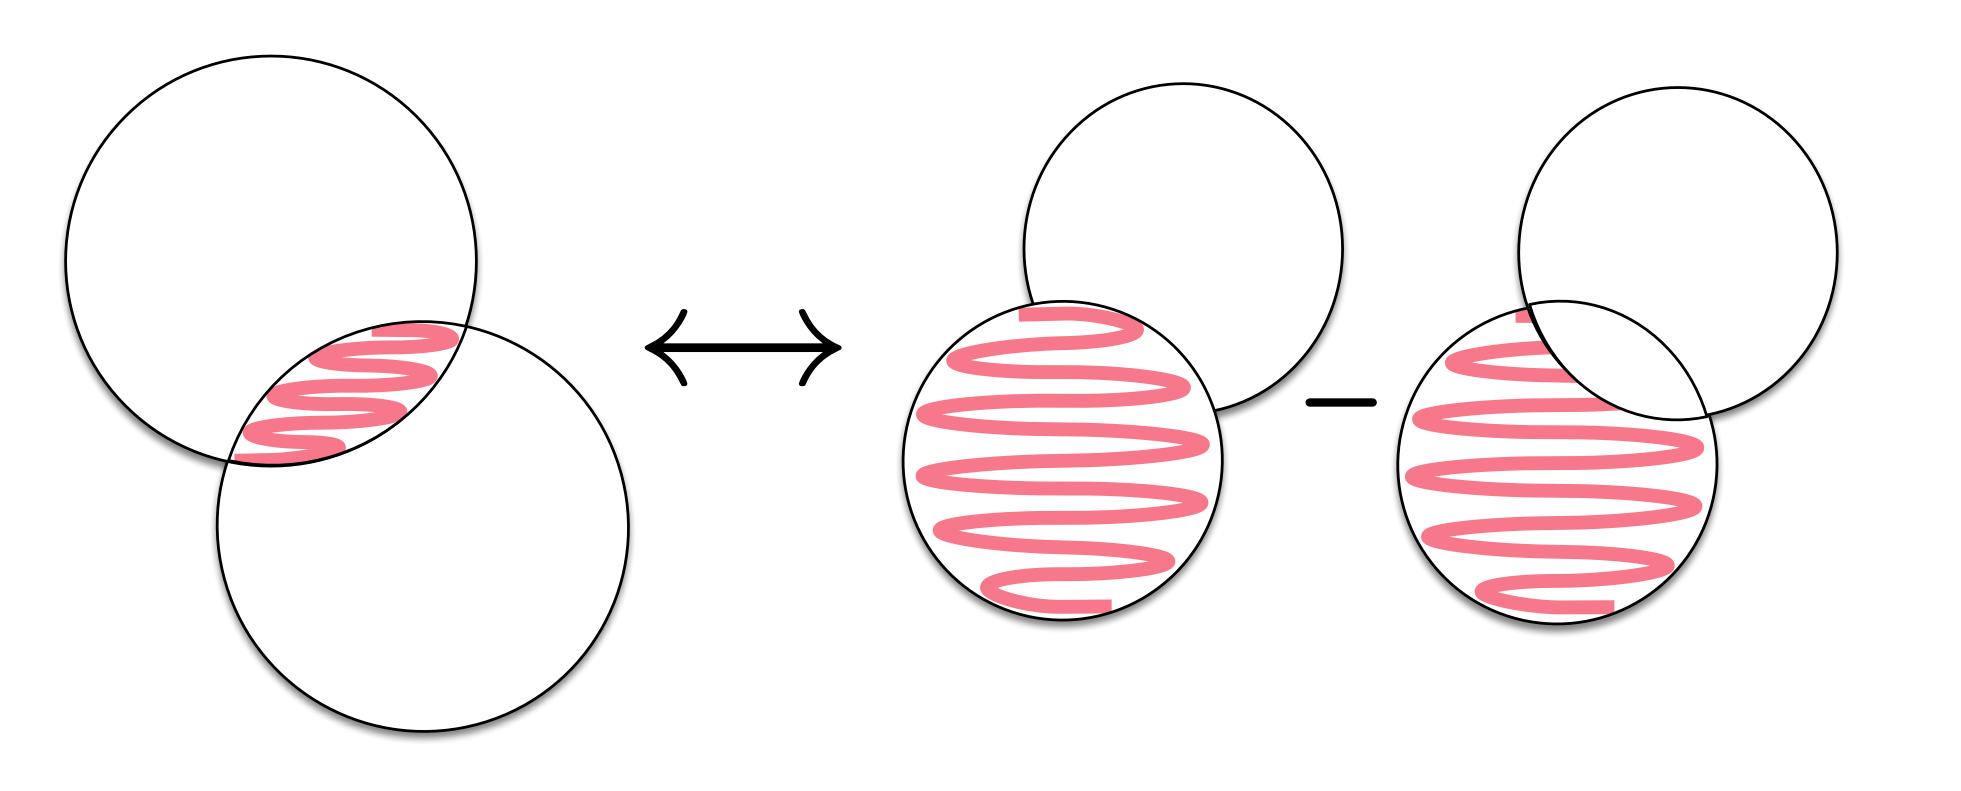
\includegraphics[width=12cm]{images/intersection1.png}
\caption{Venn-Diagram showing the definition of Intersection in terms of Set Difference}
\end{figure}
        
    \vspace{0.1in}
    
     \textbf{Part 4} \\
    Explain the difference between DRC and TRC.
    
    \vspace{0.1in}
        \solution \\
In Tuple Relational Calculus (TRC), the variables typically range over tuples, i.e. they directly represent tuples. On the other hand, in Domain Relational Calculus (DRC), the variables range over domain elements, i.e. field values. In TRC, tuples are semantically equivalent to variables, i.e. field referencing can be used to select tuple parts. On the other hand, in DRC, formal variables are explicit and have to be defined.
    \vspace{0.1in}
    
    
\end{homeworkProblem}   

\begin{homeworkProblem}

\textbf{Part 1} \\

The names of the seas that are deeper than 3000 mt and into which at least one river finally flows.

\vspace{0.1in}
    \solution \\
      
    $<name> \mid \exists depth, rname, river, lake, sea, length, sLong, sLat, mount, sAlt, estLong, estLat \\
    Sea(name, depth) \wedge  \\ River(rname, river, lake, sea, length, sLong, sLat, mount, sAlt, estLong, estLat) \wedge \\ depth > 3000 \wedge sea = name$ 
    \vspace{0.1in}
    
\textbf{Part 2} \\
The names of the groups of islands that consist only of islands that are neither 'volcanic' nor
'coral'.

 \vspace{0.1in}
    \solution \\ \\    
   %SOLUTION
   $<islands> \mid \exists name, area, height, type, long, lat \\
Island(name, islands, area, height, type, long, lat) \wedge \\
type \notin \{volcanic, coral\} \wedge islands \neq \emptyset  $
    \vspace{0.1in}    

\textbf{Part 3} \\
The name of the mountain, the name of the mountains where it belongs to and the name of
the country where the mountain is located for each mountain that is located on an island
that is of type 'coral'.

 
 \vspace{0.1in} 
     \solution \\ \\ 
     %SOLUTION   
     $<moiMountain, mMountains, gmCountry> \mid \exists \\ moiIsland, mHeight, mType, mLong, mLat, \\ iIslands, iArea, iHeight, iType, iLong, iLat, gmProvince \\
mountainOnIsland(moiMountain, moiIsland) \wedge \\ Mountain(moiMountain, mMountains, mHeight, mType, mLong, mLat) \wedge \\ geo\_Mountain(moiMountain, gmCountry, gmProvince)  \wedge \\
Island(moiIsland, iIslands, iArea, iHeight, iType, iLong, iLat) \wedge iType \neq "coral" $

     \vspace{0.1in}

    
\textbf{Part 4} \\
Give the name and country name of all cities with a population higher than 500,000.

 \vspace{0.1in} 
     \solution \\ \\    
    %SOLUTION
   $<cName, coName> \mid \exists cCountry, cProvince, cPopulation, cLong, cLat, \\
   coCapital, coProvince, coArea, coPopulation \\
City(cName, cCountry, cProvince, cPopulation, cLong, cLat)  \wedge \\
Country(cCountry, coName, coCapital, coProvince, coArea, coPopulation) \wedge \\
cPopulation > 500000 $
 
    \vspace{0.1in}
        
\end{homeworkProblem}

\begin{homeworkProblem}
Suppose you have a file of 15,000 pages and eight buffer pages and you are sorting it using general
(external) merge-sort. Please answer the following questions: \\

\textbf{Part 1} \\
How many runs will you produce? Remark: When a file is sorted, in intermediate steps
subfiles are created. Each sorted subfile is called a run. See also slide 35 in Chapter 2.
 \textbf{Note: Detailed solution of Q3 is produced in \textit{Figures 2, 3 and 4.}}
 
 \vspace{0.1in} 
     \solution \\
     %SOLUTION
     \textbf{2189} runs will be produced   
     \vspace{0.1in}
     
 \textbf{Part 2} \\
How many passes will it take to sort the file completely?
 
 \vspace{0.1in} 
     \solution \\ 
    It will take \textbf{5} passes   
     \vspace{0.1in}
     
 \textbf{Part 3} \\
How many buffer pages do you need at least to sort the file in two passes? 

 \vspace{0.1in} 
     \solution \\
     With \textbf{123} buffers, you can sort the file in two passes 
     \vspace{0.1in}
 
 \textbf{Part 4} \\
How many runs and passes would a Two-Way-Sort algorithm take?
 
 \vspace{0.1in} 
     \solution \\
     %SOLUTION
     Two-Way Sort Algorithm will take \textbf{30004} runs and \textbf{15} passes   
     \vspace{0.1in}   
     
\begin{figure}[h]
\centering
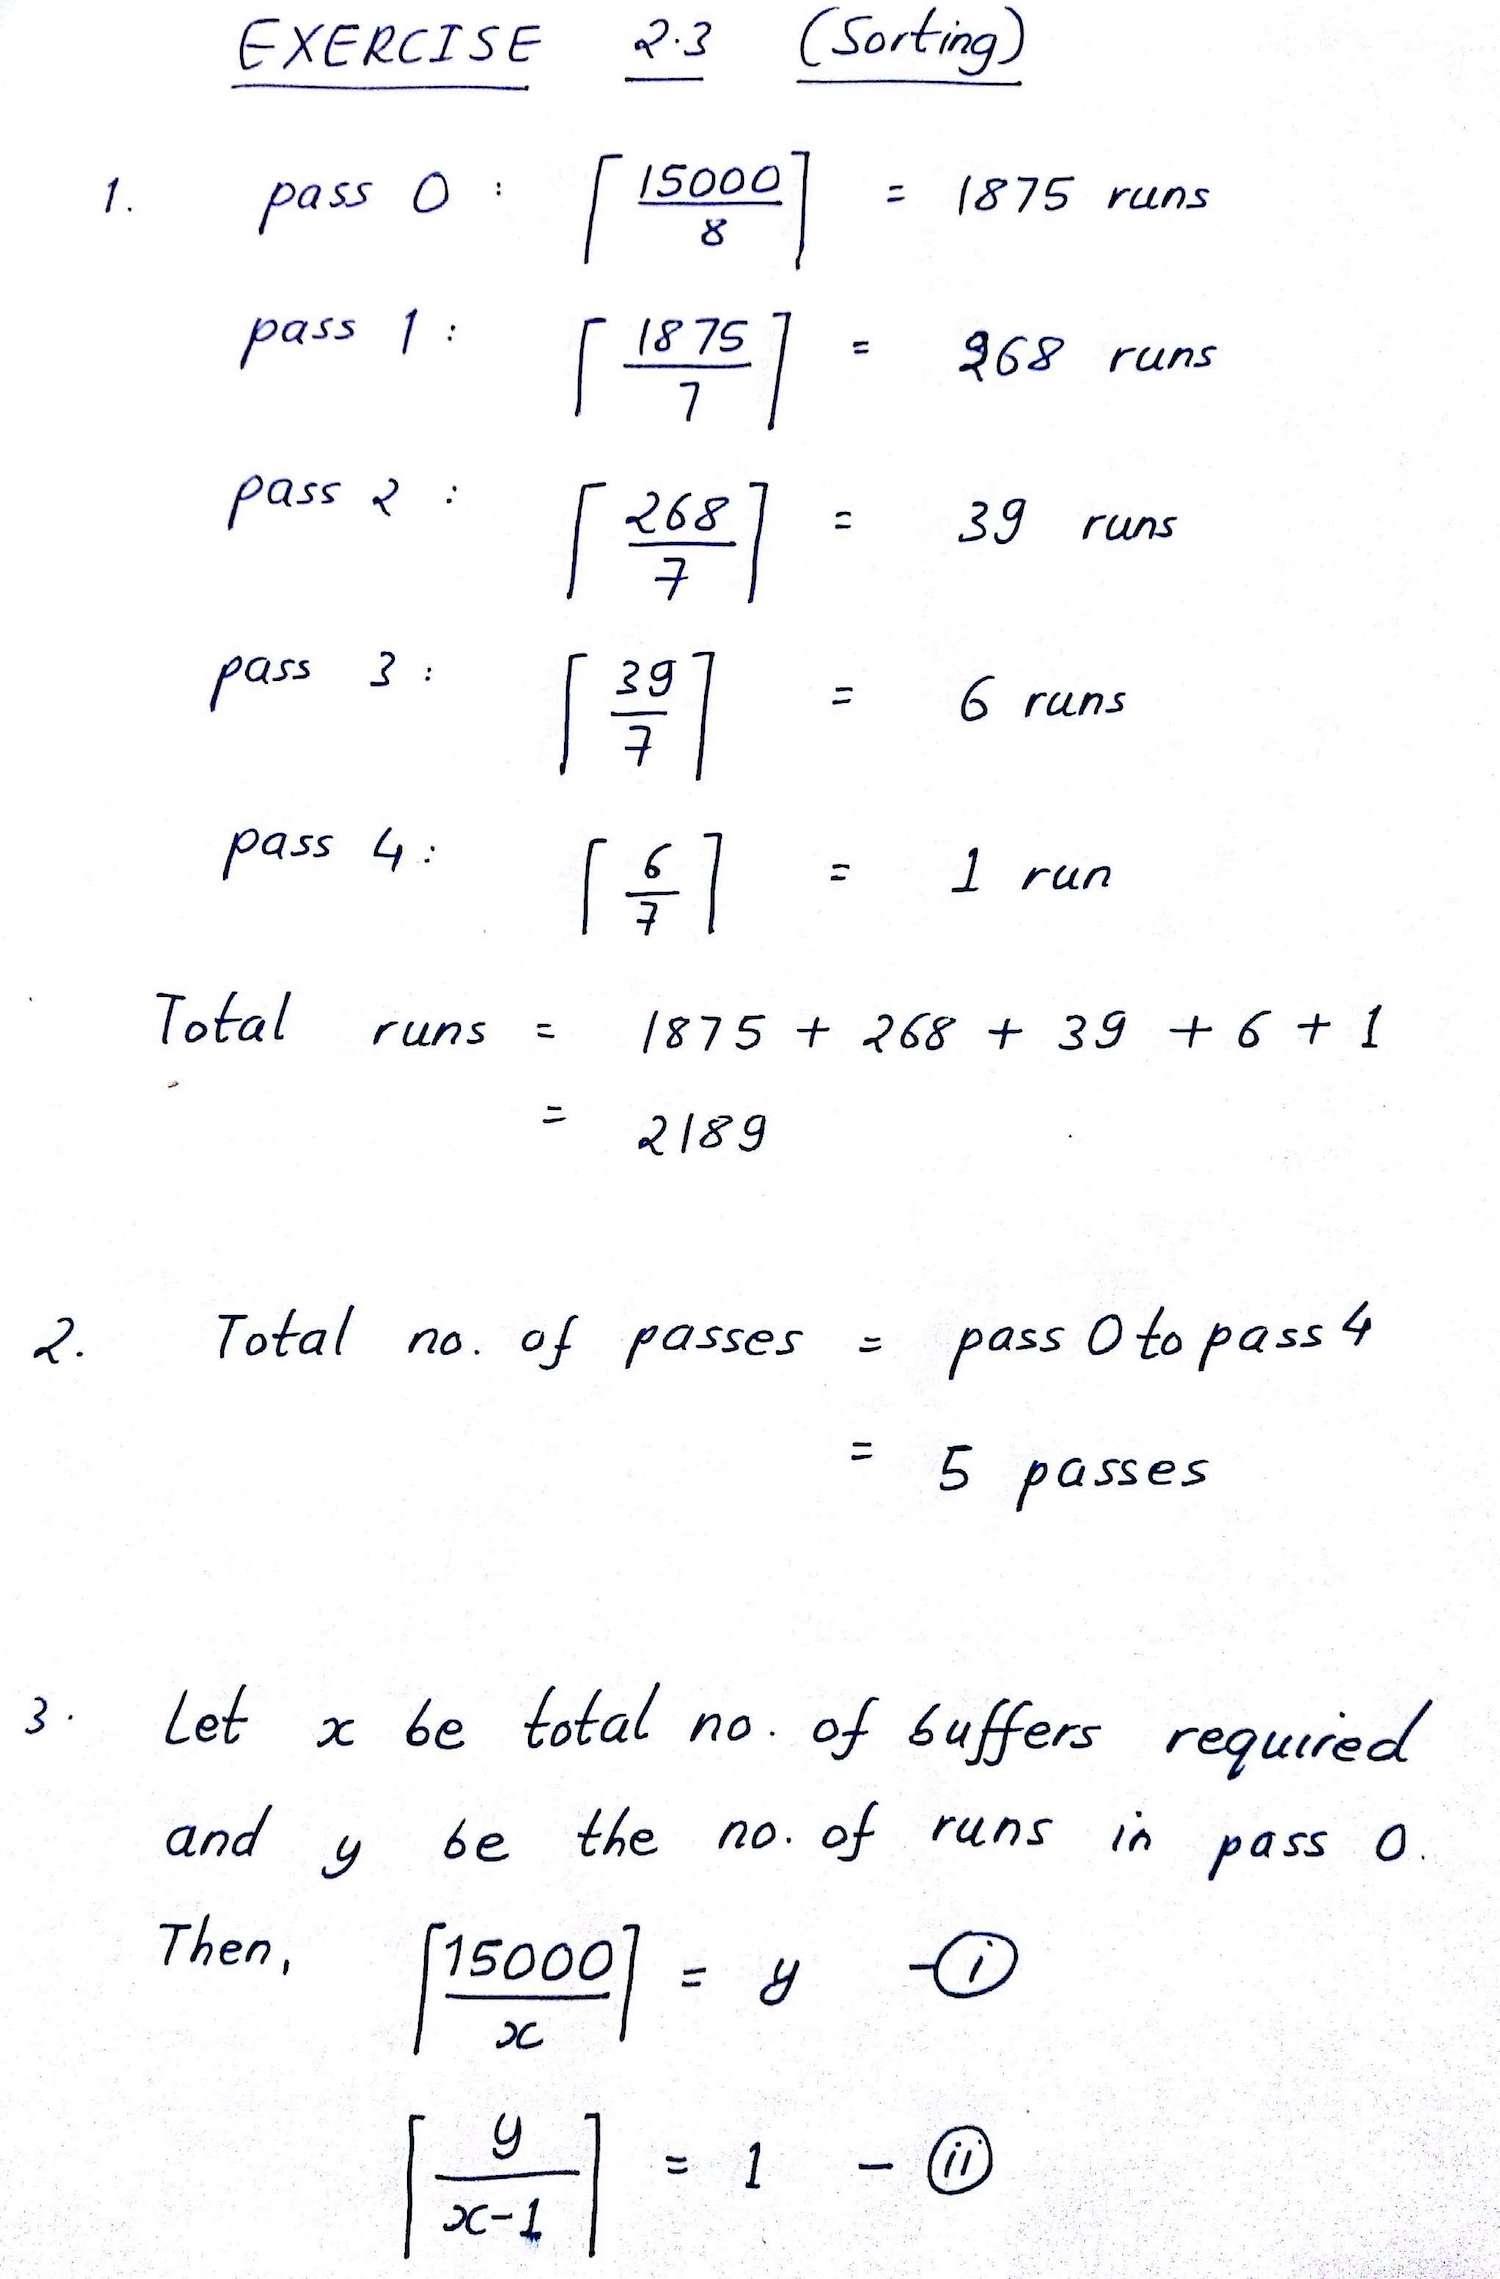
\includegraphics[width=12cm]{images/sol31.jpg}
\caption{Paper-based Solution for Question 3-1}
\end{figure} 

\begin{figure}[h]
\centering
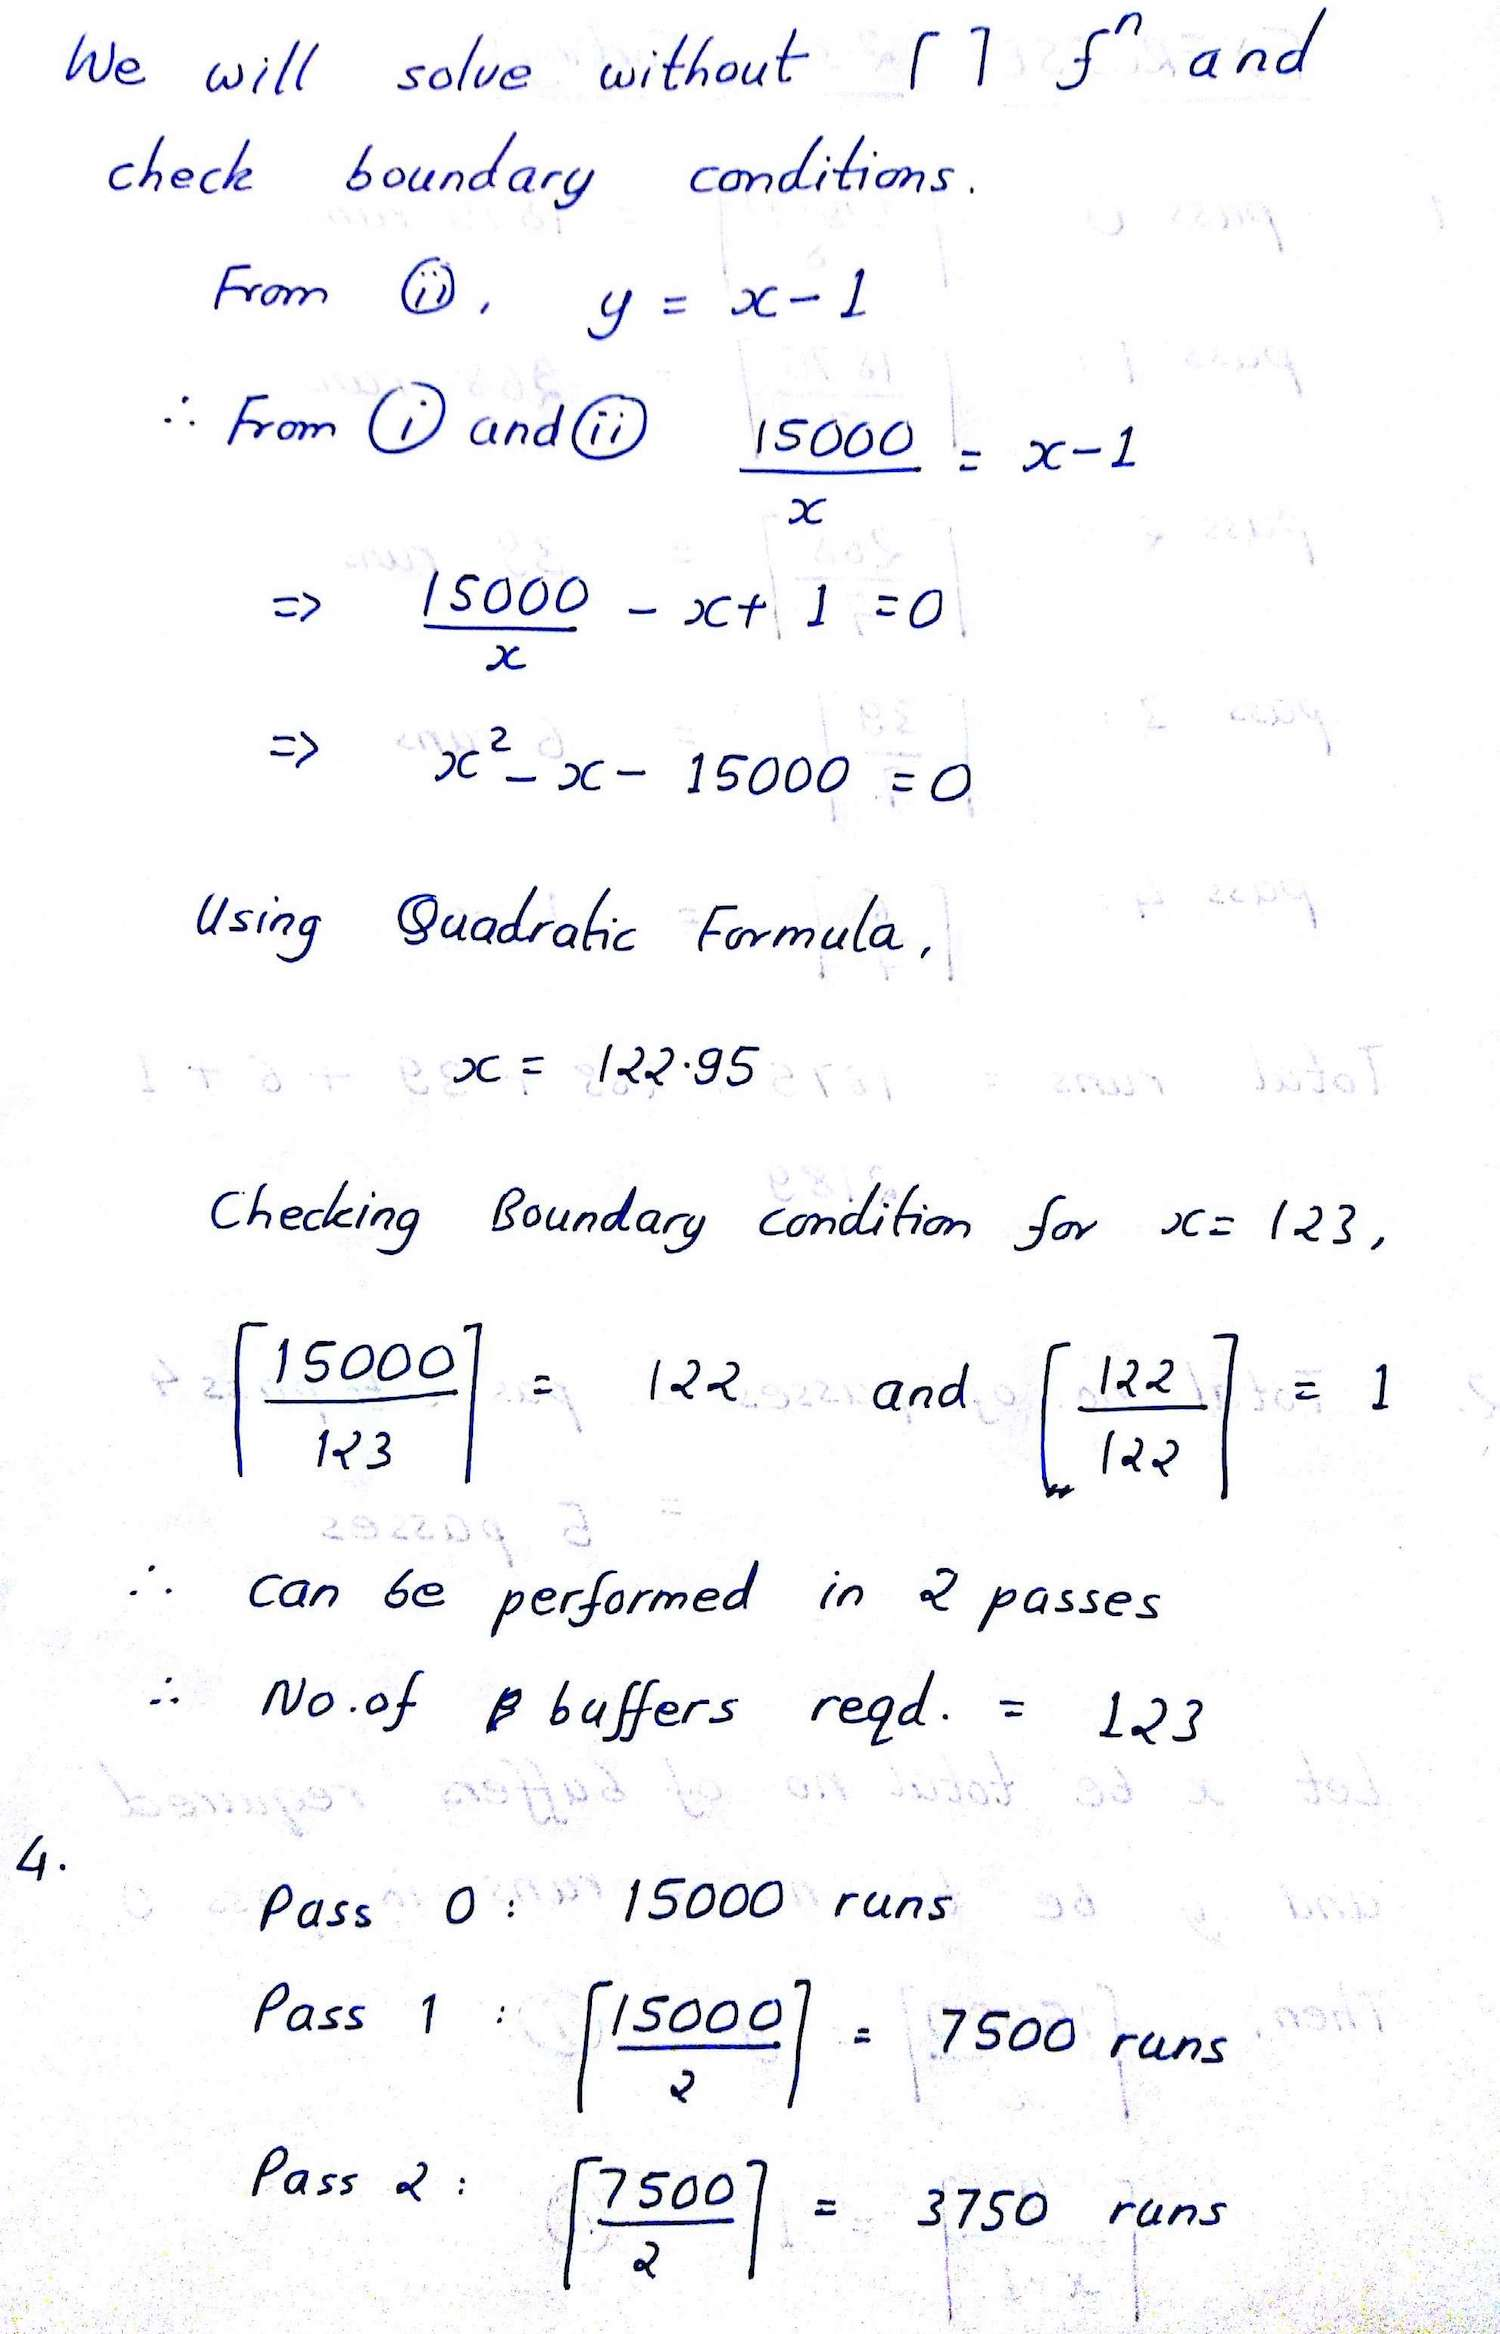
\includegraphics[width=12cm]{images/sol32.jpg}
\caption{Paper-based Solution for Question 3-2}
\end{figure} 

\begin{figure}[h]
\centering
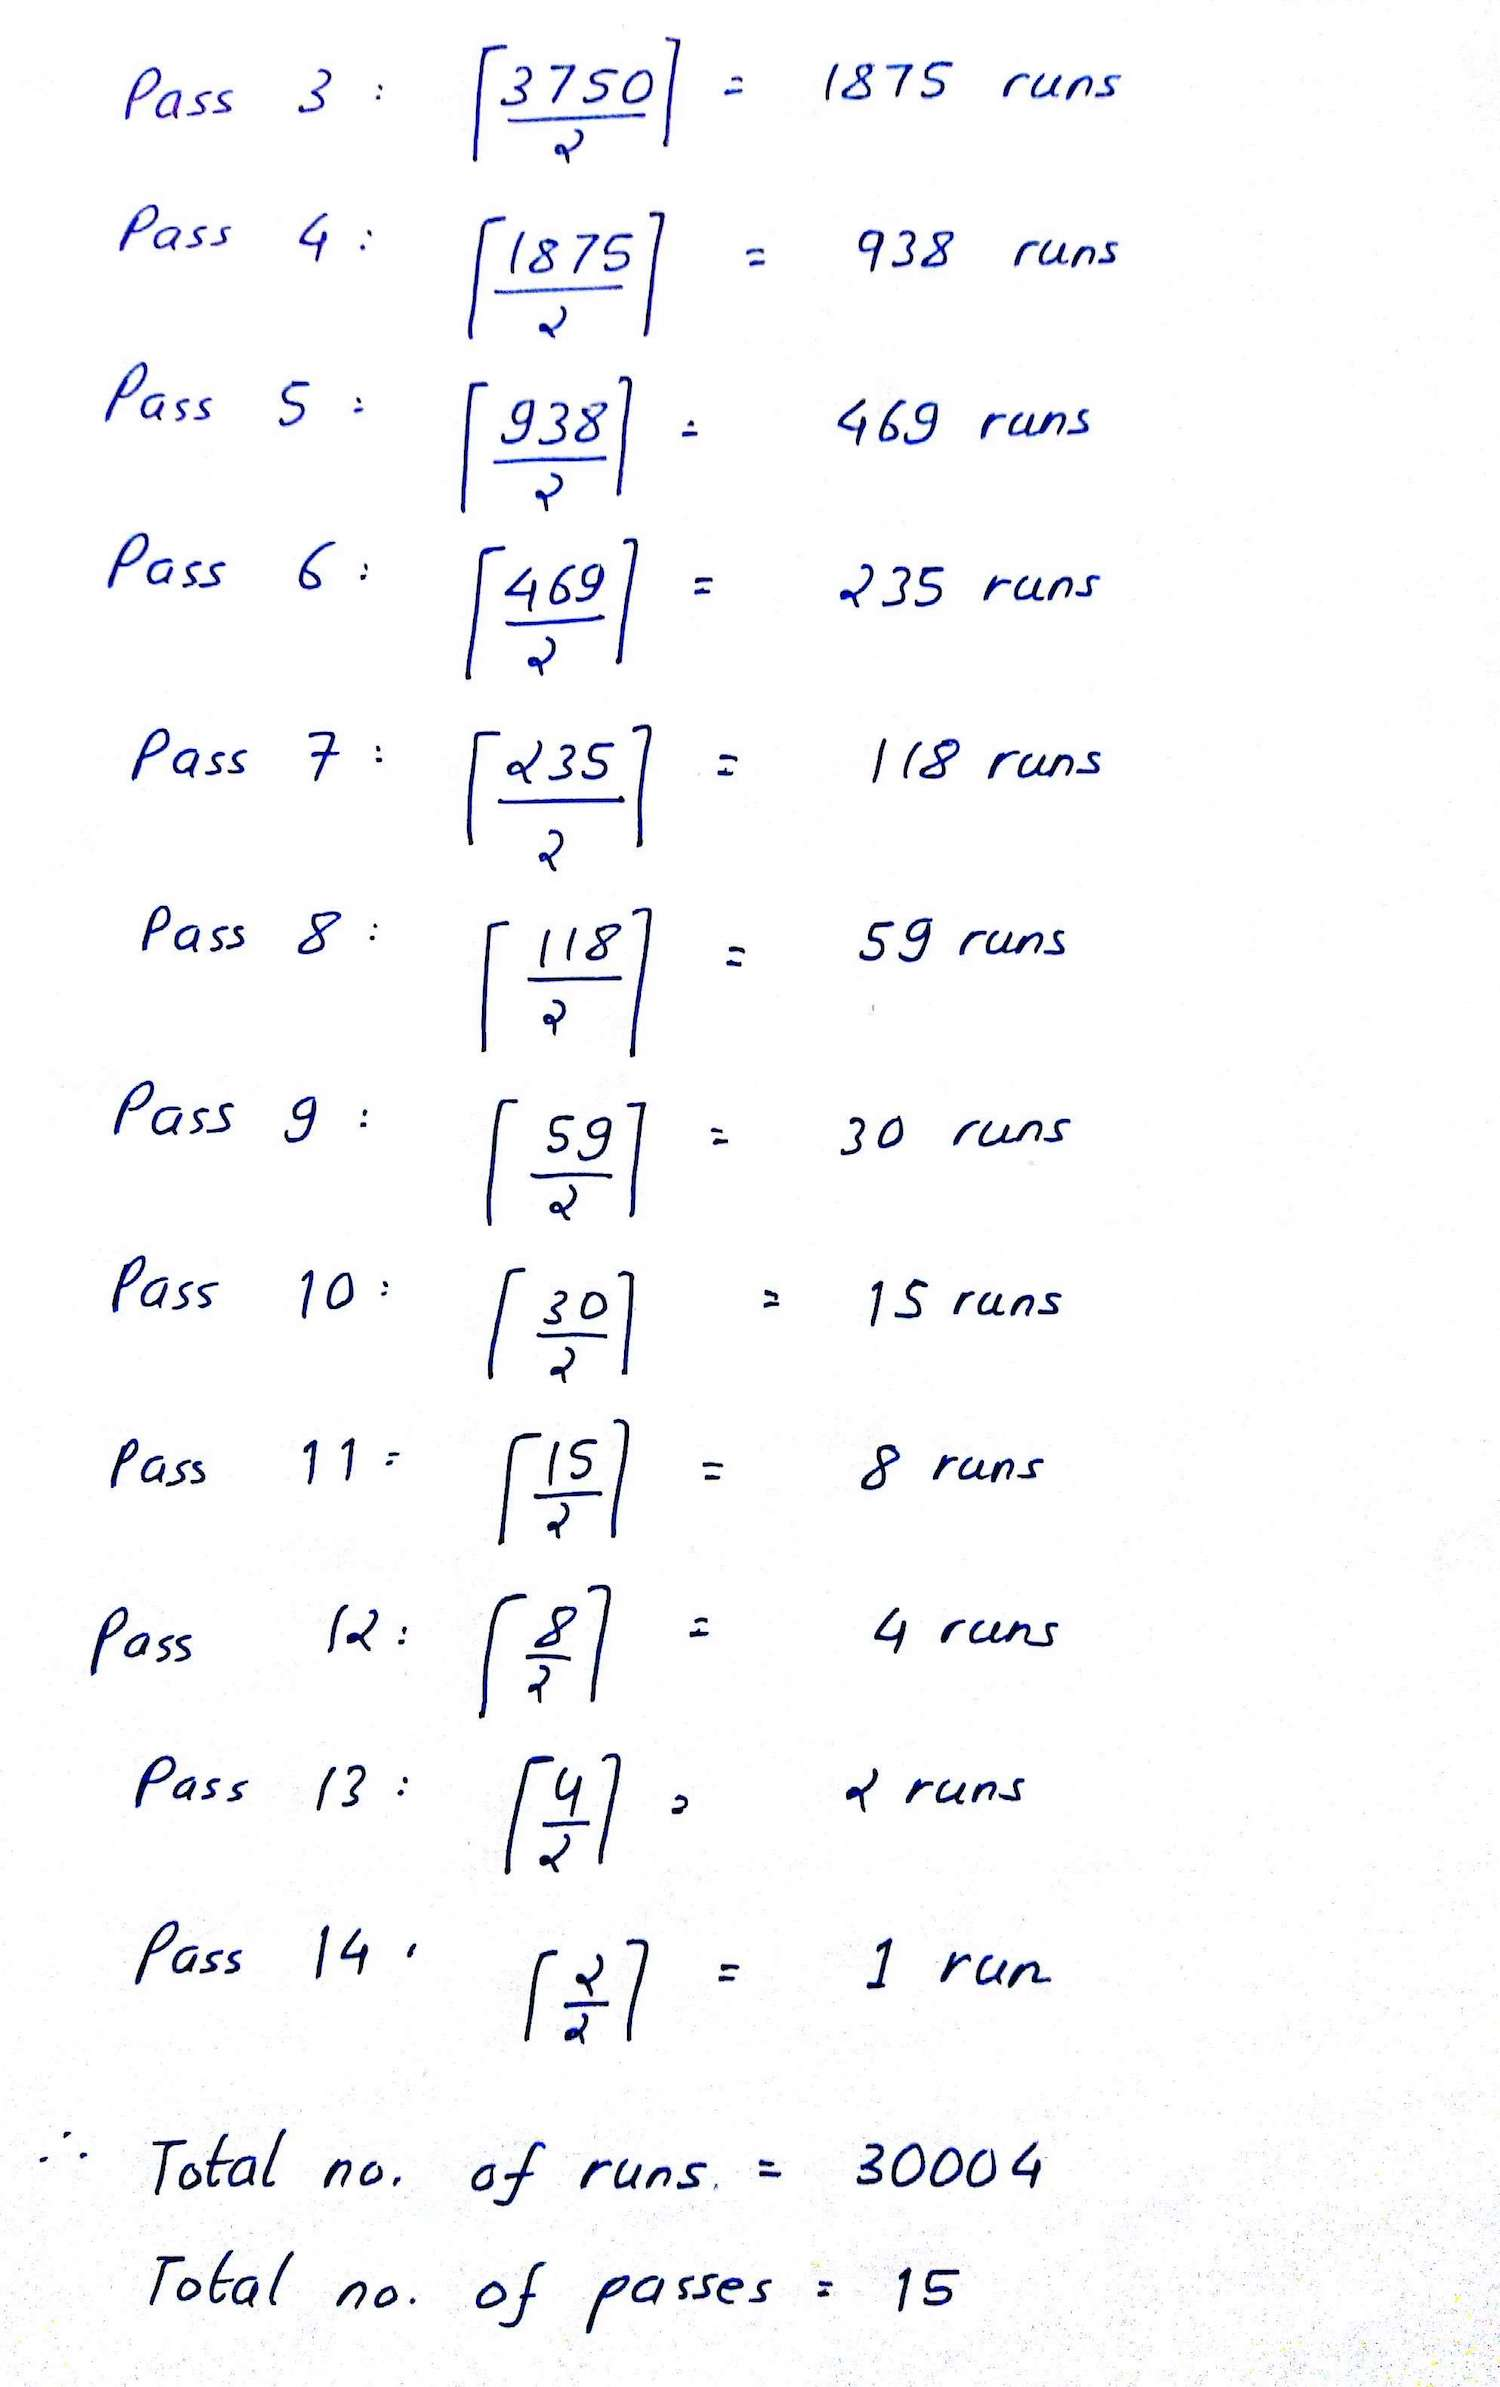
\includegraphics[width=12cm]{images/sol33.jpg}
\caption{Paper-based Solution for Question 3-3}
\end{figure} 

\end{homeworkProblem}

\begin{homeworkProblem}

\textbf{Part 1} \\
Calculate the I/O requirements of a simple nested loop join
 
 \vspace{0.1in} 
     \solution \\ \\ 
     %SOLUTION 
     In the expression below, M and N are the number of pages in the relations Album and Track respectively, $p_M$ and $p_N$ are the number of tuples in each page of the relations. \\
     
     \textbf{M as outer and N as inner relation} \\
     \textbf{Tuple-by-Tuple Simple Nested Loop Join} \\
     $M +  p_M \times M \times N$ \\
     $= 10000 + 100 \times 10000 \times 200000$ \\
     $ = 200000010000 $
          
    \vspace{0.1in}
     \textbf{Page-by-Page Simple Nested Loop Join} \\
     $M + M \times N$ \\
     $= 10000 + 10000 \times 200000$ \\
     $ = 2000010000 $
     
      \vspace{0.1in}
     \textbf{N as outer and M as inner relation} \\
     \textbf{Tuple-by-Tuple Simple Nested Loop Join} \\
     $N +  p_N \times N \times M$ \\
     $= 200000 + 80 \times 200000 \times 10000$ \\
     $ = 160000200000 $
          
    \vspace{0.1in}
     \textbf{Page-by-Page Simple Nested Loop Join} \\
     $M + M \times N$ \\
     $= 200000 + 200000 \times 10000$ \\
     $ = 2000200000 $
     \vspace{0.1in}
     
 \textbf{Part 2} \\
Calculate the I/O requirements of a block nested loop join
 
\vspace{0.1in} 
     \solution \\ \\ 
     %SOLUTION
     Block nested join for 16 buffers: \\
     
      \textbf{M as outer and N as inner relation} \\
     $ 10000 + \lceil \frac{10000}{14} \rceil \times 200000$
     $ = 143010000 $   
     \vspace{0.1in}
     
      \textbf{N as outer and M as inner relation} \\
      $ 200000 + \lceil \frac{200000}{14} \rceil \times 10000$
     $ = 143060000 $   
     \vspace{0.1in}
     
 \textbf{Part 3} \\
Explain the differences between the two algorithms. What are the similarities and differences? How does the block nested loop join reduce I/O costs?
 
 \vspace{0.1in} 
     \solution \\ \\ 
     %SOLUTION
     Tuple-at-a-time Simple Nested Loop Join scans outer relation and then for each tuple, it scans the entire inner relation. On the other hand, the page-at-a-time Simple Nested Loop Join will load the outer relation page-by-page, and then the inner relation for each page. The Block Nested Loop Join, on the other hand, scans entire inner relation for each block of pages in the outer relation. Therefore, the I/O cost of Block Nested Loop Join is lower than cost of both the Simple Nested Loop Joins. 
Moreover, the other important difference is number of buffer pages used in the algorithms. Both tuple-at-a-time nested loop and page-at-time nested loop join use 3 buffer pages to perform the join operation. 1 page as input buffer to scan outer relation,1 page as input buffer to scan inner relation  and 1 page as output buffer. Totally, 3 pages are needed for simple nested loop join. However, block nested loop join uses 1 page as input buffer to scan inner relation S and 1 page as output buffer. The other remaining buffer pages are used to load the blocks of the outer relation R. In this case, 1 buffer page is used as input buffer to scan inner relation  and 1 page as output buffer. Remaining 14 buffer pages are used to block outer relation . As seen, block nested loop join uses entire available buffer pages in the algorithm that means more efficient usage of buffer pages and causing performance increases and decreasing I/O cost. 

The similarities can be indicated as outer-inner relation usage, buffer usage and loop operations in the algorithms. 

     \vspace{0.1in}
     
\end{homeworkProblem}
     
\begin{homeworkProblem}
Given is a relation with 50.000 records. Each page for a node in a B+ tree can hold 20 pointers
to records or pages. A data page can store 20 records. \\

 \textbf{Part 1} \\
Assume that each node is 70 \% full. What is the height of the B+-tree? 

 \vspace{0.1in} 
     \solution \\ \\ 
     %SOLUTION  
     Given that the B+Tree can hold 20 pointers to pages. However, the B+ Tree has 70\% occupancy. Therefore, number of effective pointers to pages that the tree can hold,
     \begin{center} $ \implies 0.7 \times 20 = 14$ \end{center} 
Our B+ Tree can now be represented as Table 1

\begin{table}[]
\centering
\begin{tabular}{|l|l|l|l|}
\hline
Level    & Node & Entries & No. of Pointers \\ \hline
0 (Root) & 1    & 13      & 14              \\ \hline
1        & 14   & 182     & 196             \\ \hline
2        & 196  & 2548    & 2744         \\ \hline  
\end{tabular}
\caption{Different Levels of the B+ Tree}
\label{B+ Tree}
\end{table}

We have 2744 addresses in Level 2 already, which is more than 2500 pointers to pages required in the relations. \\
Therefore, the B-Tree has a depth of \textbf{3}.
Our B+ Tree has a depth of \textbf{3}
 \vspace{0.1in}
     
 \textbf{Part 2} \\
What are the I/O costs for an equality selection on a non-key attribute for the following
cases?

\begin{enumerate}[label = (\alph*)]
\item with a clustered B+-tree of height 3 (matching records are located in one page);
 
 \vspace{0.1in} 
     \solution \\ \\ 
     %SOLUTION
     The clustered index will guide the search, and after the end of the B+ tree traversal, we will need to input the correct page which contains our desired result. Therefore, total I/O is for the tree traversal and retrieving the correct page, i.e. 3 I/Os + 1 I/O = 4.
     Hence, total number of I/Os = \textbf{4} I/Os
     \vspace{0.1in}
     
\item without any index, nor is the file sorted on the attribute occurring in selection;

\vspace{0.1in} 
     \solution \\ \\ 
     %SOLUTION 
     Total number of pages at the leaf node = 2500
    If we consider that all pages need to be scanned, then the I/O costs will be \textbf{2500} I/Os. \\
    However, assuming, on an average that half the total number of pages need to be searched to find the equality results, it gives a total of 1250 I/Os.
          
     \vspace{0.1in}
     
\item with an unclustered B+-tree index of height 4, and there are 2 matching records;

\vspace{0.1in} 
     \solution \\ \\ 
     4 I/Os to traverse the tree + 2 I/Os to retrieve the matching records = \textbf{6} I/Os 
     \vspace{0.1in}

\item with an unclustered B+-tree of height 5 and three tenth of the records match the
selection.

\vspace{0.1in} 
\solution \\ \\ 
     %SOLUTION
     No. of matching records = $\frac{3}{10} \times 50000 = 15000$ records \\
     In the worst case, we need to do 15000 page I/Os, one for each record. Plus the I/Os for traversing the tree. Therefore, a total of 15000 I/Os + 5 I/Os = \textbf{15005} I/Os.   
     \vspace{0.1in}

\end{enumerate}
\end{homeworkProblem}

\end{document}
\documentclass[12pt]{article}

\usepackage{fancyhdr}
\usepackage{extramarks}
\usepackage{amsmath}
\usepackage{amsthm}
\usepackage{amsfonts}
\usepackage{tikz}
\usepackage[plain]{algorithm}
\usepackage{algpseudocode}
\usepackage[export]{adjustbox}
\usepackage[latin1]{inputenc}           %For German characters
\usepackage{enumitem}               %For changing enumeration character
\usepackage{listings}               %For code
\usepackage{csquotes}
\usepackage{graphicx}               %For graphics e.g, images

\usetikzlibrary{automata,positioning}

%
% Basic Document Settings
%

\topmargin=-0.45in
\evensidemargin=0in
\oddsidemargin=0in
\textwidth=6.5in
\textheight=9.0in
\headsep=0.25in

\linespread{1.1}

\pagestyle{fancy}
\lhead{\hmwkAuthorName}
\chead{\hmwkClass\ : \hmwkTitle}
\rhead{\firstxmark}
\lfoot{\lastxmark}
\cfoot{\thepage}

\renewcommand\headrulewidth{0.4pt}
\renewcommand\footrulewidth{0.4pt}

\setlength\parindent{0pt}

%
% Create Problem Sections
%

\newcommand{\enterProblemHeader}[1]{
    \nobreak\extramarks{}{Problem \arabic{#1} continued on next page\ldots}\nobreak{}
    \nobreak\extramarks{Problem \arabic{#1} (continued)}{Problem \arabic{#1} continued on next page\ldots}\nobreak{}
}

\newcommand{\exitProblemHeader}[1]{
    \nobreak\extramarks{Problem \arabic{#1} (continued)}{Problem \arabic{#1} continued on next page\ldots}\nobreak{}
    \stepcounter{#1}
    \nobreak\extramarks{Problem \arabic{#1}}{}\nobreak{}
}

\setcounter{secnumdepth}{0}
\newcounter{partCounter}
\newcounter{homeworkProblemCounter}
\setcounter{homeworkProblemCounter}{1}
\nobreak\extramarks{Problem \arabic{homeworkProblemCounter}}{}\nobreak{}

%
% Homework Problem Environment
%
% This environment takes an optional argument. When given, it will adjust the
% problem counter. This is useful for when the problems given for your
% assignment aren't sequential. See the last 3 problems of this template for an
% example.
%
\newenvironment{homeworkProblem}[1][-1]{
    \ifnum#1>0
        \setcounter{homeworkProblemCounter}{#1}
    \fi
    \section{Problem \arabic{homeworkProblemCounter}}
    \setcounter{partCounter}{1}
    \enterProblemHeader{homeworkProblemCounter}
}{
    \exitProblemHeader{homeworkProblemCounter}
}

%
% Homework Details
%   - Title
%   - Due date
%   - Class
%   - Section/Time
%   - Instructor
%   - Author
%

\newcommand{\hmwkTitle}{Assignment\ \#2}
\newcommand{\hmwkDueDate}{November 15, 2016}
\newcommand{\hmwkClass}{Implementation of Databases}
\newcommand{\hmwkAuthorName}{Sanchit Alekh}
\newcommand{\hmwkClassTime}{MSc. Software Systems Engineering}
\newcommand{\hmwkClassInstructor}{Universitätsprofessor Dr. rer. pol. Matthias Jarke}
\newcommand{\hmwkClassInstructors}{Dr. rer. nat. Christoph Quix}

%
% Title Page
%



\title{
   \begin{center}
   \vspace*{-20mm}
   
\includegraphics[width=0.4\textwidth, right]{images/rwth_logo.png}
   \\
   \vspace*{3cm}
    \textmd{\textbf{\hmwkClass}}\\
    \textmd{\textbf{\hmwkTitle}}\\
    \normalsize\vspace{0.1in}\small{Due\ on\ \hmwkDueDate } \\
    \vspace{0.1in}\large{\textit{\hmwkClassInstructor}} \\
    \vspace{0.1in}\large{\textit{\hmwkClassInstructors}} \\
    \vspace{3in}
     \textbf{Submitted by:} \\
     \vspace{0.25in}
    \large{Sanchit Alekh, Idil Esen Zülfikar, Nihal Hegde} \\
    %\author{\textbf{\hmwkAuthorName}}
    \vspace{0.1in} \large{\textit{\hmwkClassTime}} \\
    %\vspace{0.1in} \large{\textit{Matrikelnummer : 359831}}
    \end{center}
    }


\date{}

\renewcommand{\part}[1]{\textbf{\large Part \Alph{partCounter}}\stepcounter{partCounter}\\}

%
% Various Helper Commands
%

% Useful for algorithms
\newcommand{\alg}[1]{\textsc{\bfseries \footnotesize #1}}

% For derivatives
\newcommand{\deriv}[1]{\frac{\mathrm{d}}{\mathrm{d}x} (#1)}

% For partial derivatives
\newcommand{\pderiv}[2]{\frac{\partial}{\partial #1} (#2)}

% Integral dx
\newcommand{\dx}{\mathrm{d}x}

% Alias for the Solution section header
\newcommand{\solution}{\textbf{\large Solution}}

% Probability commands: Expectation, Variance, Covariance, Bias
\newcommand{\E}{\mathrm{E}}
\newcommand{\Var}{\mathrm{Var}}
\newcommand{\Cov}{\mathrm{Cov}}
\newcommand{\Bias}{\mathrm{Bias}}

\begin{document}

\maketitle

\pagebreak

\begin{homeworkProblem}
    
    \textbf{Part 1} \\
    Variants of relational algebra are used internally in DBMS to represent queries and query evaluation plans. Please explain, why relational algebra is suitable for this?
    
    \vspace{0.1in}
    \solution \\
    One of the most desirable properties of Relational Algebra is that queries are composed using a collection of operators, and every operator accepts one or two relation instances as arguments and returns a relation instance as the result. This property makes extremely easy and efficient to compose operators to form a complex query. A relational algebra expression can be recursively defined to be a relation, a unary algebra operator applied to a single expression, or a binary algebra operator applied to two expressions. 
This procedural nature of relational algebra is the main reason why it is used internally in DBMS to represent queries and evaluation plans. The approach allows us to think of an algebra expression as an imperative execution plan for a declarative SQL query. It can be used for evaluating a query, and relational systems in fact use algebra expressions to represent query evaluation plans.
        
    \vspace{0.1in}
    
    \textbf{Part 2} \\
    What does \enquote{relational completeness} mean (in your own words, please)? Show that SQL is
relationally complete by enumerating SQL constructs corresponding to selection, projection,
cartesian product, union, and difference.
    
    \vspace{0.1in}
    \solution \\
    \enquote{Relational Completeness} of a query methodology means that each and every query that can be expressed using that methodology, can also be expressed as a relational algebra query. In this case, SQL is referred to as \enquote*{Relationally Complete} because every legal construct in SQL can be expressed as a Relational Algebra query.
        
These are the examples of Relational Algebra expressions and their equivalent expressions in SQL. The following examples are derived from the \textit{Mondial} database.

\begin{itemize}

\item \textbf{SELECTION} \\
Relational Algebra: $ \sigma_{Area > 650} (Island)$ \\
SQL:  \textit{Select * From Island Where Area $>$ 650;}

\item \textbf{PROJECTION} \\
Relational Algebra: $ \pi_{Name, Islands, Area, Height} (Island)$ \\
SQL: \textit{Select Name, Islands, Area, Height From Island;}

\item \textbf{CARTESIAN PRODUCT} \\
Relational Algebra:  $ Island \times islandIn$ \\
SQL: \textit{Select * From Island CROSS JOIN islandIn;}

\item \textbf{UNION} \\
Relational Algebra:  $ \pi_{name} (Desert) \cup \pi_{name} (geo\_Desert)$ \\
SQL: \textit{Select name From Desert or Select name From geo\_Desert}

\item \textbf{SET DIFFERENCE} \\
Relational Algebra: $ \pi_{name} (\sigma_{height > 5000} (Mountain)) - \pi_{name}( \sigma_{type > 'volcanic')} (Mountain) $ \\
SQL: \textit{Select name From Mountain where height $>$ 5000 MINUS Select name From Mountain where type='volcanic'}
\end{itemize}
        
    \vspace{0.1in}
        
     \textbf{Part 3} \\
    Explain how the intersection operator is used in relational algebra. What is important for
its usage? Is it omittable (i.e., could you express it by other operators)? If so, please give
the corresponding relational algebra.
    
    \vspace{0.1in}
    \solution \\
    The \enquote*{Intersection} operator is represented in Relational Algebra with the help of the $\cap$ symbol. Although it is not a fundamental set-operator, it is an extremely widely used operation, and it is helpful to define it separately. An example use of the intersection operator is as follows:
    
    \begin{center} $ \pi_{name} (Desert) \cap \pi_{name} (geo\_Desert) $ \end{center}
    
The important condition for using the \textit{Intersection} operator is that the two sets which have to be intersected must be \textit{union-compatible}. This follows from the fact that intersection is defined in terms of set difference.

Yes, Intersection is not a fundamental set-operator, and it can be expressed in terms of the set-difference operator. Therefore, it is omittable. A general expression for the intersection operator in terms of the set-difference operator is:

    \begin{center} $ A \cup B \leftrightarrow A \setminus ( A \setminus B) $ \end{center}
    
Therefore, the example Relational Algebra query illustrated above can be represented by the equivalent query without the use of set-intersection as follows:

    \begin{center} $ \pi_{name} (Desert) - (\pi_{name} (Desert) - \pi_{name} (geo\_Desert))$ \end{center}
    
\begin{figure}[h]
\centering
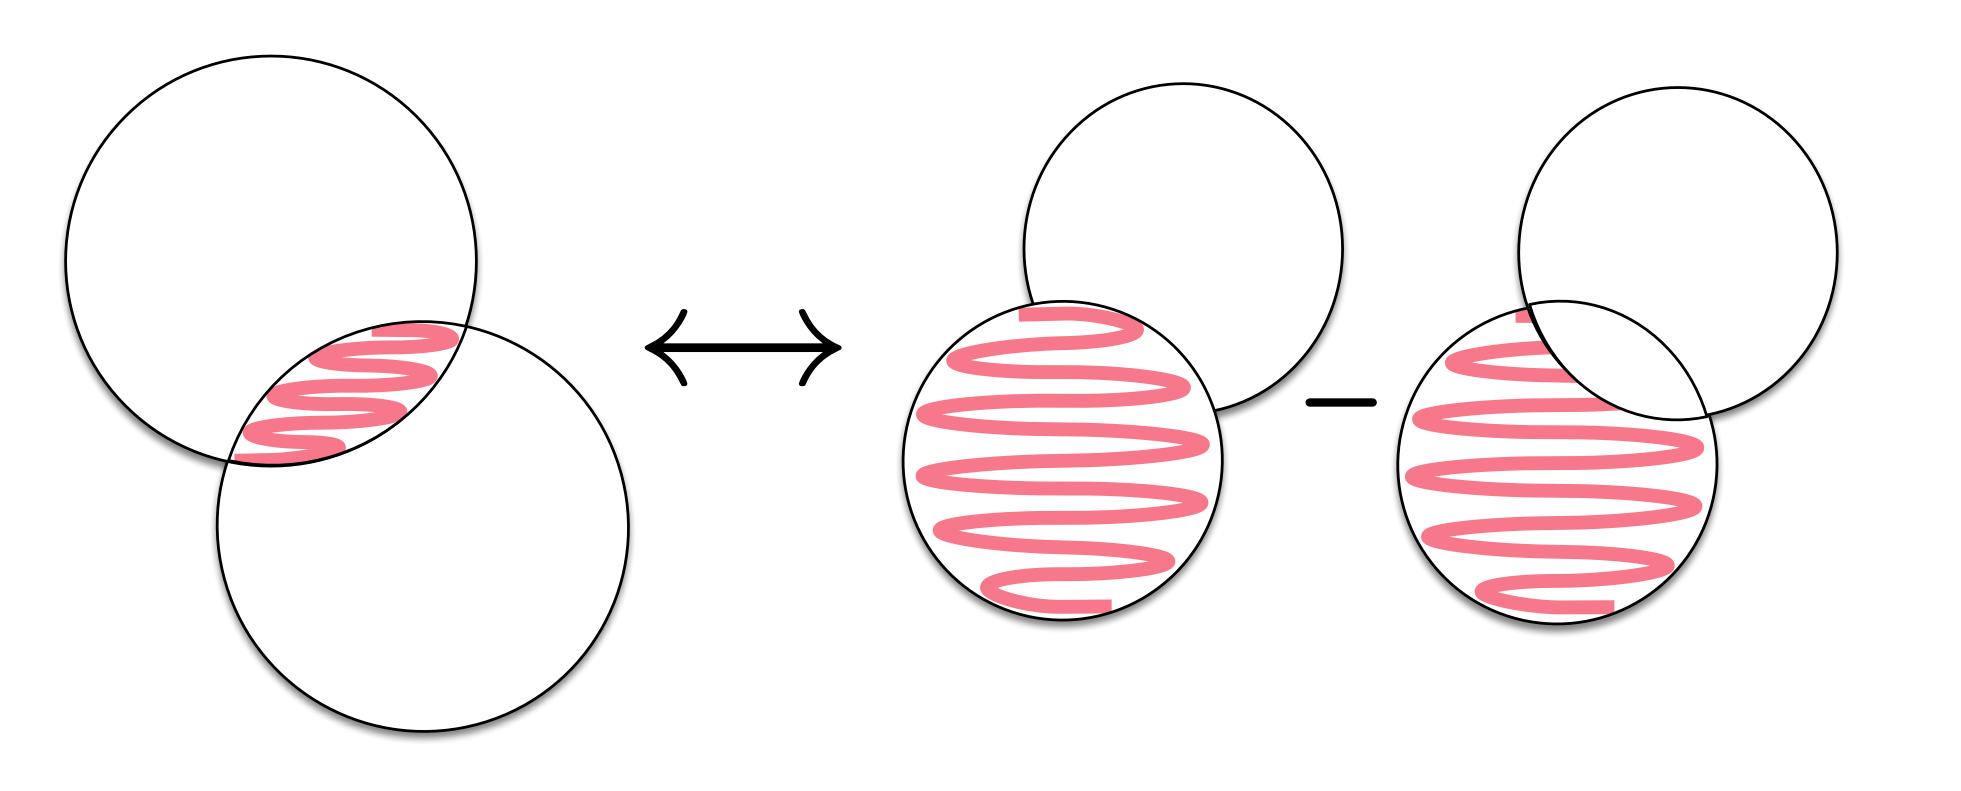
\includegraphics[width=12cm]{images/intersection1.png}
\caption{Venn-Diagram showing the definition of Intersection in terms of Set Difference}
\end{figure}
        
    \vspace{0.1in}
    
     \textbf{Part 4} \\
    Explain the difference between DRC and TRC.
    
    \vspace{0.1in}
        \solution \\
In Tuple Relational Calculus (TRC), the variables typically range over tuples, i.e. they directly represent tuples. On the other hand, in Domain Relational Calculus (DRC), the variables range over domain elements, i.e. field values. In TRC, tuples are semantically equivalent to variables, i.e. field referencing can be used to select tuple parts. On the other hand, in DRC, formal variables are explicit and have to be defined.
    \vspace{0.1in}
    
    
\end{homeworkProblem}   

\begin{homeworkProblem}

\textbf{Part 1} \\

The names of the seas that are deeper than 3000 mt and into which at least one river finally flows.

\vspace{0.1in}
    \solution \\
      
    $<name> \mid \exists depth, rname, river, lake, sea, length, sLong, sLat, mount, sAlt, estLong, estLat \\
    Sea(name, depth) \wedge  \\ River(rname, river, lake, sea, length, sLong, sLat, mount, sAlt, estLong, estLat) \wedge \\ depth > 3000 \wedge sea = name$ 
    \vspace{0.1in}
    
\textbf{Part 2} \\
The names of the groups of islands that consist only of islands that are neither 'volcanic' nor
'coral'.

 \vspace{0.1in}
    \solution \\ \\    
   %SOLUTION
   $<islands> \mid \exists name, area, height, type, long, lat \\
Island(name, islands, area, height, type, long, lat) \wedge \\
type \notin \{volcanic, coral\} \wedge islands \neq \emptyset  $
    \vspace{0.1in}    

\textbf{Part 3} \\
The name of the mountain, the name of the mountains where it belongs to and the name of
the country where the mountain is located for each mountain that is located on an island
that is of type 'coral'.

 
 \vspace{0.1in} 
     \solution \\ \\ 
     %SOLUTION   
     $<moiMountain, mMountains, gmCountry> \mid \exists \\ moiIsland, mHeight, mType, mLong, mLat, \\ iIslands, iArea, iHeight, iType, iLong, iLat, gmProvince \\
mountainOnIsland(moiMountain, moiIsland) \wedge \\ Mountain(moiMountain, mMountains, mHeight, mType, mLong, mLat) \wedge \\ geo\_Mountain(moiMountain, gmCountry, gmProvince)  \wedge \\
Island(moiIsland, iIslands, iArea, iHeight, iType, iLong, iLat) \wedge iType \neq "coral" $

     \vspace{0.1in}

    
\textbf{Part 4} \\
Give the name and country name of all cities with a population higher than 500,000.

 \vspace{0.1in} 
     \solution \\ \\    
    %SOLUTION
   $<cName, coName> \mid \exists cCountry, cProvince, cPopulation, cLong, cLat, \\
   coCapital, coProvince, coArea, coPopulation \\
City(cName, cCountry, cProvince, cPopulation, cLong, cLat)  \wedge \\
Country(cCountry, coName, coCapital, coProvince, coArea, coPopulation) \wedge \\
cPopulation > 500000 $
 
    \vspace{0.1in}
        
\end{homeworkProblem}

\begin{homeworkProblem}
Suppose you have a file of 15,000 pages and eight buffer pages and you are sorting it using general
(external) merge-sort. Please answer the following questions: \\

\textbf{Part 1} \\
How many runs will you produce? Remark: When a file is sorted, in intermediate steps
subfiles are created. Each sorted subfile is called a run. See also slide 35 in Chapter 2.
 \textbf{Note: Detailed solution of Q3 is produced in \textit{Figures 2, 3 and 4.}}
 
 \vspace{0.1in} 
     \solution \\
     %SOLUTION
     \textbf{2189} runs will be produced   
     \vspace{0.1in}
     
 \textbf{Part 2} \\
How many passes will it take to sort the file completely?
 
 \vspace{0.1in} 
     \solution \\ 
    It will take \textbf{5} passes   
     \vspace{0.1in}
     
 \textbf{Part 3} \\
How many buffer pages do you need at least to sort the file in two passes? 

 \vspace{0.1in} 
     \solution \\
     With \textbf{123} buffers, you can sort the file in two passes 
     \vspace{0.1in}
 
 \textbf{Part 4} \\
How many runs and passes would a Two-Way-Sort algorithm take?
 
 \vspace{0.1in} 
     \solution \\
     %SOLUTION
     Two-Way Sort Algorithm will take \textbf{30004} runs and \textbf{15} passes   
     \vspace{0.1in}   
     
\begin{figure}[h]
\centering
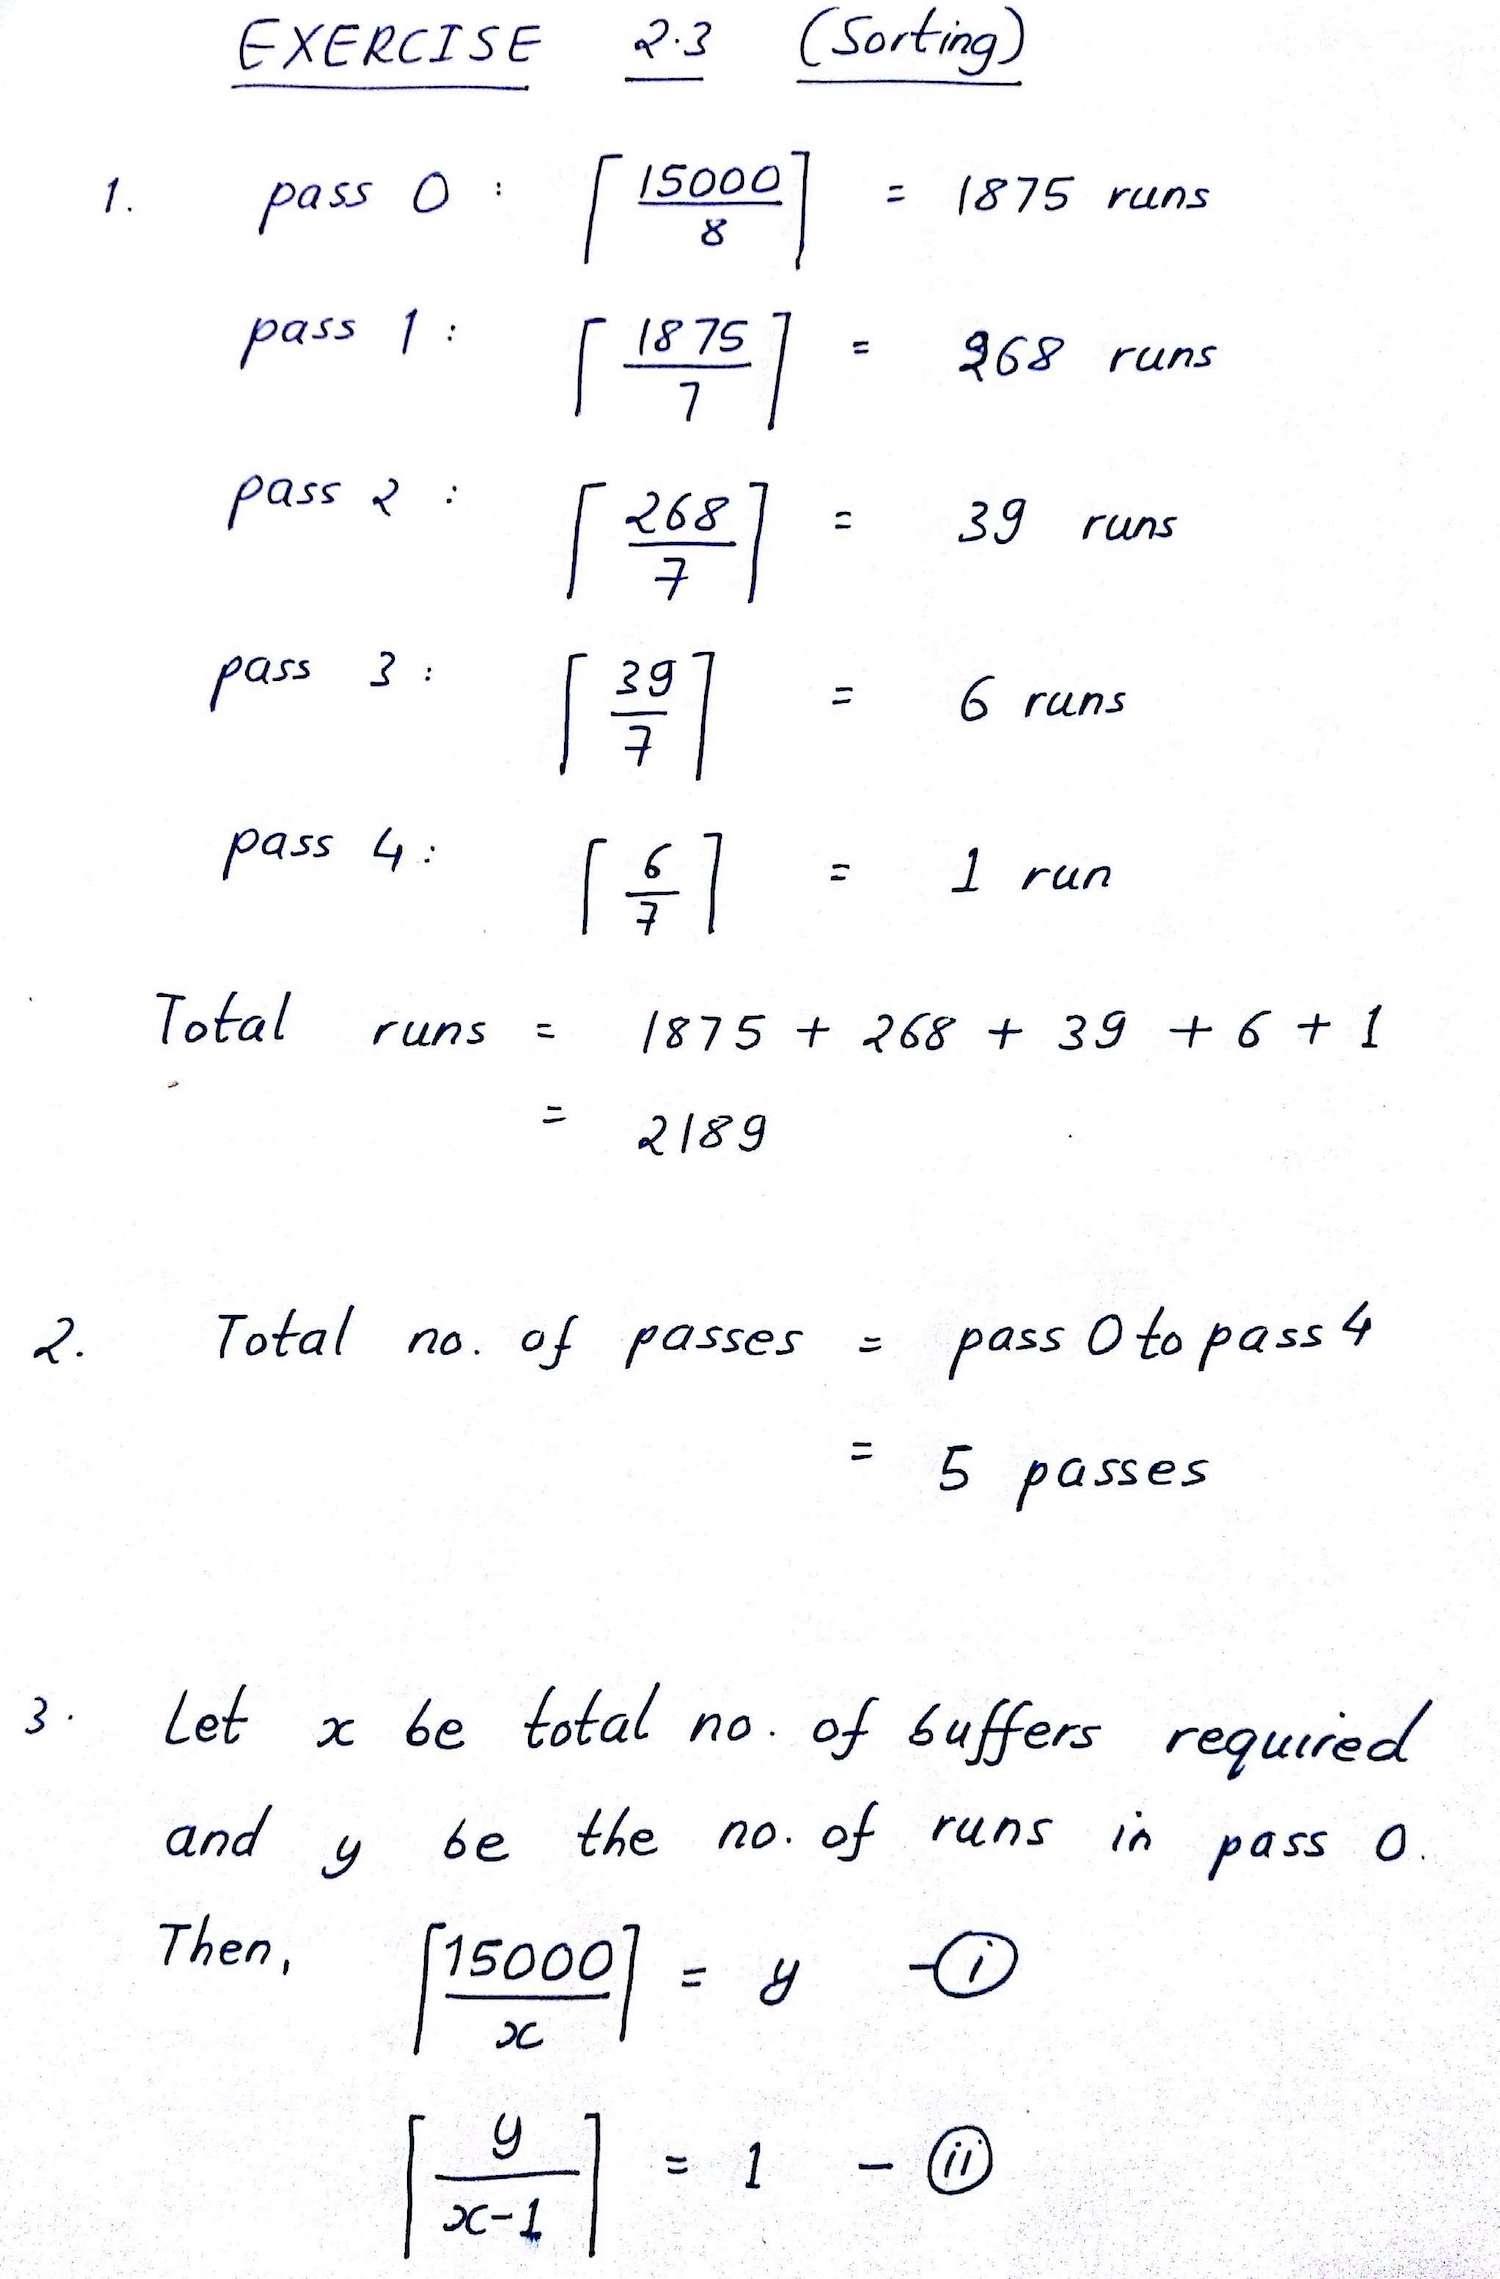
\includegraphics[width=12cm]{images/sol31.jpg}
\caption{Paper-based Solution for Question 3-1}
\end{figure} 

\begin{figure}[h]
\centering
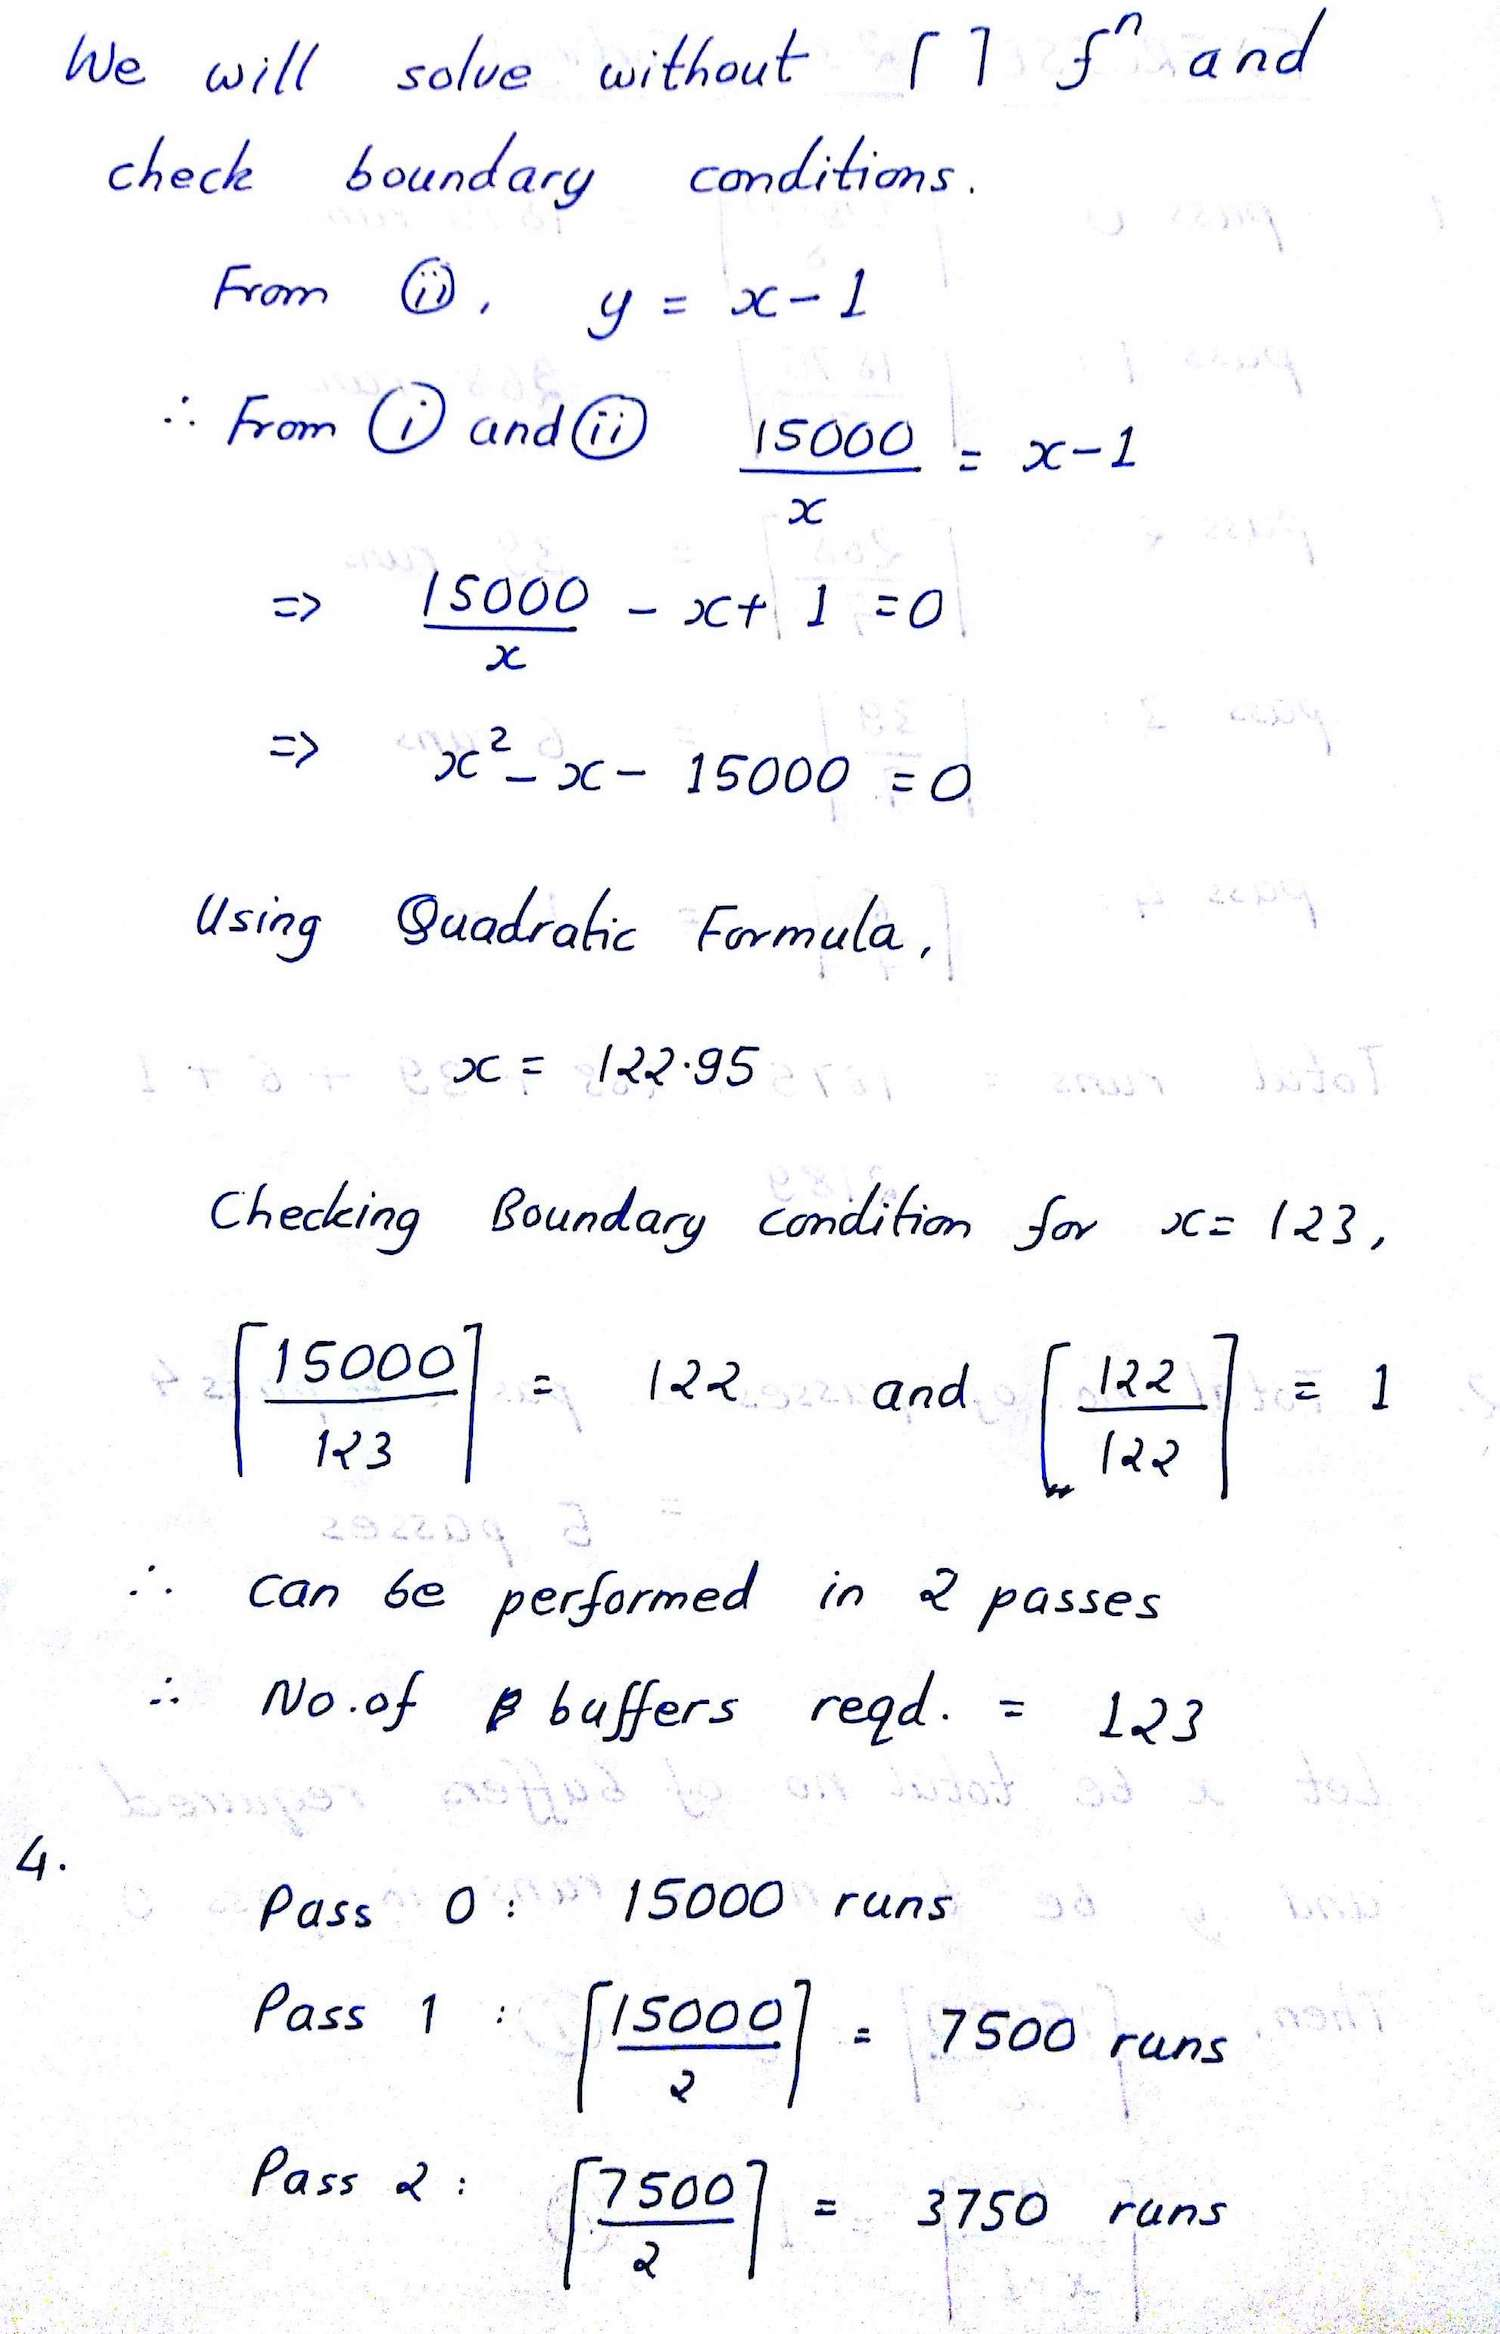
\includegraphics[width=12cm]{images/sol32.jpg}
\caption{Paper-based Solution for Question 3-2}
\end{figure} 

\begin{figure}[h]
\centering
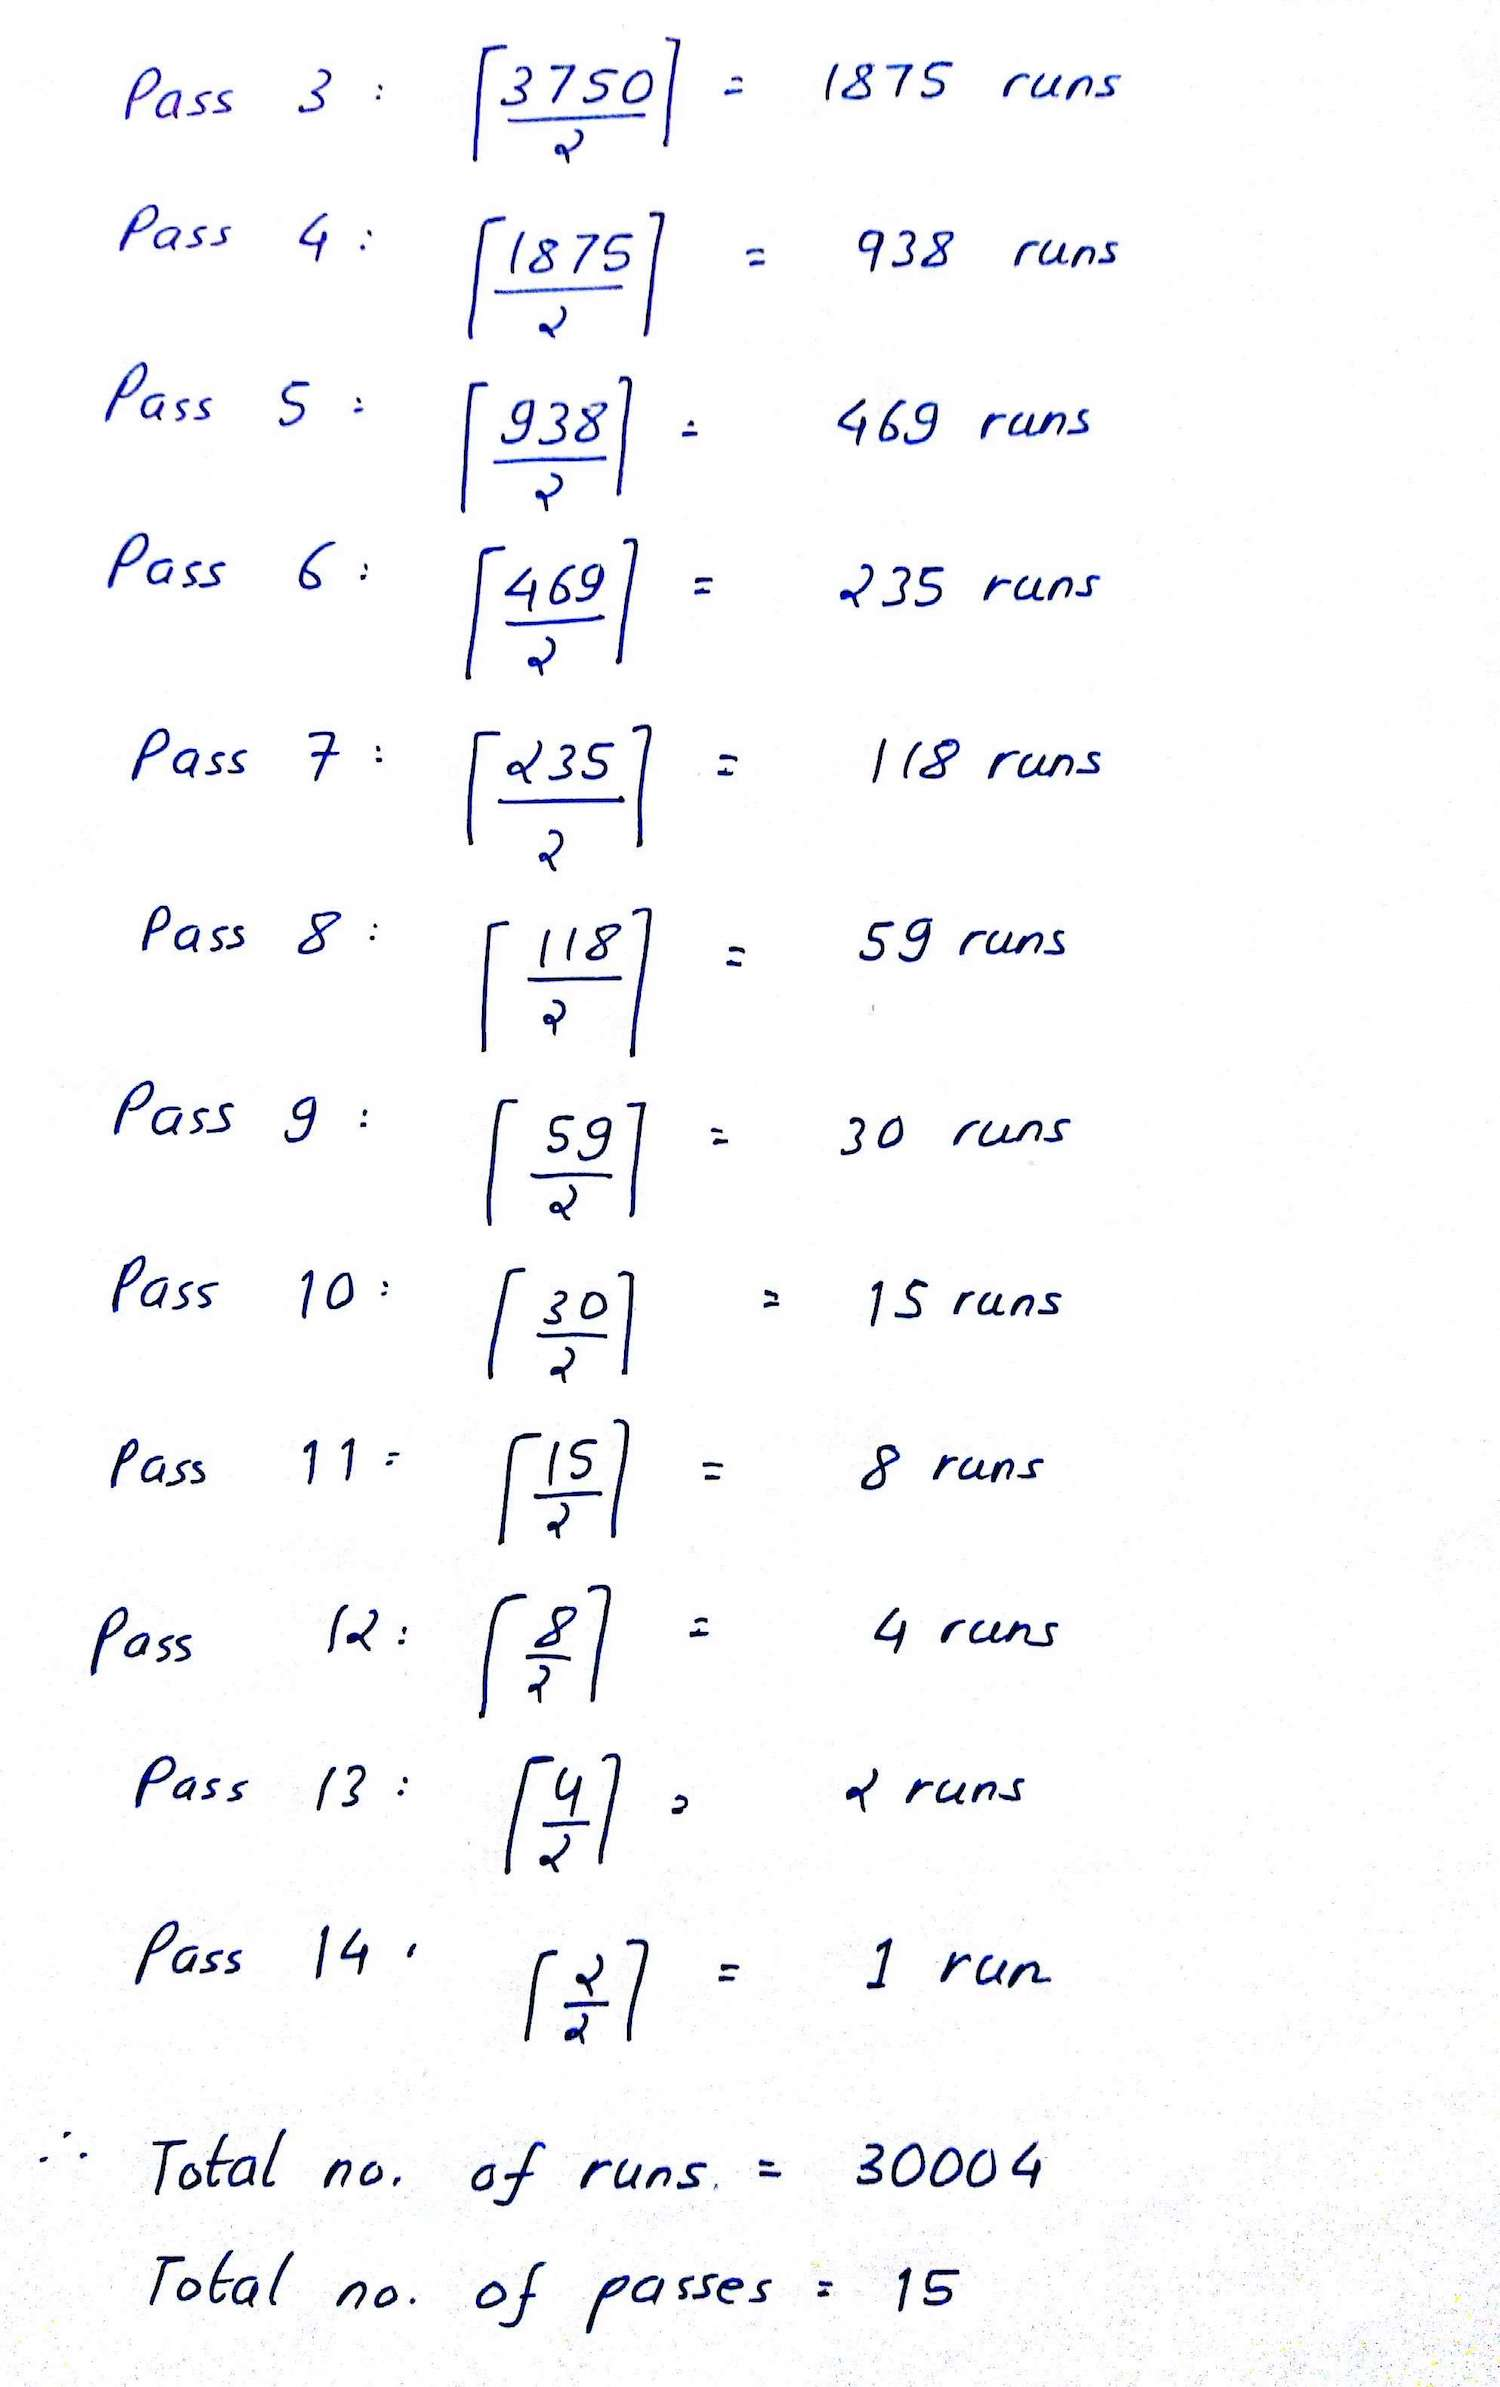
\includegraphics[width=12cm]{images/sol33.jpg}
\caption{Paper-based Solution for Question 3-3}
\end{figure} 

\end{homeworkProblem}

\begin{homeworkProblem}

\textbf{Part 1} \\
Calculate the I/O requirements of a simple nested loop join
 
 \vspace{0.1in} 
     \solution \\ \\ 
     %SOLUTION 
     In the expression below, M and N are the number of pages in the relations Album and Track respectively, $p_M$ and $p_N$ are the number of tuples in each page of the relations. \\
     
     \textbf{M as outer and N as inner relation} \\
     \textbf{Tuple-by-Tuple Simple Nested Loop Join} \\
     $M +  p_M \times M \times N$ \\
     $= 10000 + 100 \times 10000 \times 200000$ \\
     $ = 200000010000 $
          
    \vspace{0.1in}
     \textbf{Page-by-Page Simple Nested Loop Join} \\
     $M + M \times N$ \\
     $= 10000 + 10000 \times 200000$ \\
     $ = 2000010000 $
     
      \vspace{0.1in}
     \textbf{N as outer and M as inner relation} \\
     \textbf{Tuple-by-Tuple Simple Nested Loop Join} \\
     $N +  p_N \times N \times M$ \\
     $= 200000 + 80 \times 200000 \times 10000$ \\
     $ = 160000200000 $
          
    \vspace{0.1in}
     \textbf{Page-by-Page Simple Nested Loop Join} \\
     $M + M \times N$ \\
     $= 200000 + 200000 \times 10000$ \\
     $ = 2000200000 $
     \vspace{0.1in}
     
 \textbf{Part 2} \\
Calculate the I/O requirements of a block nested loop join
 
\vspace{0.1in} 
     \solution \\ \\ 
     %SOLUTION
     Block nested join for 16 buffers: \\
     
      \textbf{M as outer and N as inner relation} \\
     $ 10000 + \lceil \frac{10000}{14} \rceil \times 200000$
     $ = 143010000 $   
     \vspace{0.1in}
     
      \textbf{N as outer and M as inner relation} \\
      $ 200000 + \lceil \frac{200000}{14} \rceil \times 10000$
     $ = 143060000 $   
     \vspace{0.1in}
     
 \textbf{Part 3} \\
Explain the differences between the two algorithms. What are the similarities and differences? How does the block nested loop join reduce I/O costs?
 
 \vspace{0.1in} 
     \solution \\ \\ 
     %SOLUTION
     Tuple-at-a-time Simple Nested Loop Join scans outer relation and then for each tuple, it scans the entire inner relation. On the other hand, the page-at-a-time Simple Nested Loop Join will load the outer relation page-by-page, and then the inner relation for each page. The Block Nested Loop Join, on the other hand, scans entire inner relation for each block of pages in the outer relation. Therefore, the I/O cost of Block Nested Loop Join is lower than cost of both the Simple Nested Loop Joins. 
Moreover, the other important difference is number of buffer pages used in the algorithms. Both tuple-at-a-time nested loop and page-at-time nested loop join use 3 buffer pages to perform the join operation. 1 page as input buffer to scan outer relation,1 page as input buffer to scan inner relation  and 1 page as output buffer. Totally, 3 pages are needed for simple nested loop join. However, block nested loop join uses 1 page as input buffer to scan inner relation S and 1 page as output buffer. The other remaining buffer pages are used to load the blocks of the outer relation R. In this case, 1 buffer page is used as input buffer to scan inner relation  and 1 page as output buffer. Remaining 14 buffer pages are used to block outer relation . As seen, block nested loop join uses entire available buffer pages in the algorithm that means more efficient usage of buffer pages and causing performance increases and decreasing I/O cost. 

The similarities can be indicated as outer-inner relation usage, buffer usage and loop operations in the algorithms. 

     \vspace{0.1in}
     
\end{homeworkProblem}
     
\begin{homeworkProblem}
Given is a relation with 50.000 records. Each page for a node in a B+ tree can hold 20 pointers
to records or pages. A data page can store 20 records. \\

 \textbf{Part 1} \\
Assume that each node is 70 \% full. What is the height of the B+-tree? 

 \vspace{0.1in} 
     \solution \\ \\ 
     %SOLUTION  
     Given that the B+Tree can hold 20 pointers to pages. However, the B+ Tree has 70\% occupancy. Therefore, number of effective pointers to pages that the tree can hold,
     \begin{center} $ \implies 0.7 \times 20 = 14$ \end{center} 
Our B+ Tree can now be represented as Table 1

\begin{table}[]
\centering
\begin{tabular}{|l|l|l|l|}
\hline
Level    & Node & Entries & No. of Pointers \\ \hline
0 (Root) & 1    & 13      & 14              \\ \hline
1        & 14   & 182     & 196             \\ \hline
2        & 196  & 2548    & 2744         \\ \hline  
\end{tabular}
\caption{Different Levels of the B+ Tree}
\label{B+ Tree}
\end{table}

We have 2744 addresses in Level 2 already, which is more than 2500 pointers to pages required in the relations. \\
Therefore, the B-Tree has a depth of \textbf{3}.
Our B+ Tree has a depth of \textbf{3}
 \vspace{0.1in}
     
 \textbf{Part 2} \\
What are the I/O costs for an equality selection on a non-key attribute for the following
cases?

\begin{enumerate}[label = (\alph*)]
\item with a clustered B+-tree of height 3 (matching records are located in one page);
 
 \vspace{0.1in} 
     \solution \\ \\ 
     %SOLUTION
     The clustered index will guide the search, and after the end of the B+ tree traversal, we will need to input the correct page which contains our desired result. Therefore, total I/O is for the tree traversal and retrieving the correct page, i.e. 3 I/Os + 1 I/O = 4.
     Hence, total number of I/Os = \textbf{4} I/Os
     \vspace{0.1in}
     
\item without any index, nor is the file sorted on the attribute occurring in selection;

\vspace{0.1in} 
     \solution \\ \\ 
     %SOLUTION 
     Total number of pages at the leaf node = 2500
    If we consider that all pages need to be scanned, then the I/O costs will be \textbf{2500} I/Os. \\
    However, assuming, on an average that half the total number of pages need to be searched to find the equality results, it gives a total of 1250 I/Os.
          
     \vspace{0.1in}
     
\item with an unclustered B+-tree index of height 4, and there are 2 matching records;

\vspace{0.1in} 
     \solution \\ \\ 
     4 I/Os to traverse the tree + 2 I/Os to retrieve the matching records = \textbf{6} I/Os 
     \vspace{0.1in}

\item with an unclustered B+-tree of height 5 and three tenth of the records match the
selection.

\vspace{0.1in} 
\solution \\ \\ 
     %SOLUTION
     No. of matching records = $\frac{3}{10} \times 50000 = 15000$ records \\
     In the worst case, we need to do 15000 page I/Os, one for each record. Plus the I/Os for traversing the tree. Therefore, a total of 15000 I/Os + 5 I/Os = \textbf{15005} I/Os.   
     \vspace{0.1in}

\end{enumerate}
\end{homeworkProblem}

\end{document}
\documentclass[12pt]{article}

\usepackage{fancyhdr}
\usepackage{extramarks}
\usepackage{amsmath}
\usepackage{amsthm}
\usepackage{amsfonts}
\usepackage{tikz}
\usepackage[plain]{algorithm}
\usepackage{algpseudocode}
\usepackage[export]{adjustbox}
\usepackage[latin1]{inputenc}           %For German characters
\usepackage{enumitem}               %For changing enumeration character
\usepackage{listings}               %For code
\usepackage{csquotes}
\usepackage{graphicx}               %For graphics e.g, images

\usetikzlibrary{automata,positioning}

%
% Basic Document Settings
%

\topmargin=-0.45in
\evensidemargin=0in
\oddsidemargin=0in
\textwidth=6.5in
\textheight=9.0in
\headsep=0.25in

\linespread{1.1}

\pagestyle{fancy}
\lhead{\hmwkAuthorName}
\chead{\hmwkClass\ : \hmwkTitle}
\rhead{\firstxmark}
\lfoot{\lastxmark}
\cfoot{\thepage}

\renewcommand\headrulewidth{0.4pt}
\renewcommand\footrulewidth{0.4pt}

\setlength\parindent{0pt}

%
% Create Problem Sections
%

\newcommand{\enterProblemHeader}[1]{
    \nobreak\extramarks{}{Problem \arabic{#1} continued on next page\ldots}\nobreak{}
    \nobreak\extramarks{Problem \arabic{#1} (continued)}{Problem \arabic{#1} continued on next page\ldots}\nobreak{}
}

\newcommand{\exitProblemHeader}[1]{
    \nobreak\extramarks{Problem \arabic{#1} (continued)}{Problem \arabic{#1} continued on next page\ldots}\nobreak{}
    \stepcounter{#1}
    \nobreak\extramarks{Problem \arabic{#1}}{}\nobreak{}
}

\setcounter{secnumdepth}{0}
\newcounter{partCounter}
\newcounter{homeworkProblemCounter}
\setcounter{homeworkProblemCounter}{1}
\nobreak\extramarks{Problem \arabic{homeworkProblemCounter}}{}\nobreak{}

%
% Homework Problem Environment
%
% This environment takes an optional argument. When given, it will adjust the
% problem counter. This is useful for when the problems given for your
% assignment aren't sequential. See the last 3 problems of this template for an
% example.
%
\newenvironment{homeworkProblem}[1][-1]{
    \ifnum#1>0
        \setcounter{homeworkProblemCounter}{#1}
    \fi
    \section{Problem \arabic{homeworkProblemCounter}}
    \setcounter{partCounter}{1}
    \enterProblemHeader{homeworkProblemCounter}
}{
    \exitProblemHeader{homeworkProblemCounter}
}

%
% Homework Details
%   - Title
%   - Due date
%   - Class
%   - Section/Time
%   - Instructor
%   - Author
%

\newcommand{\hmwkTitle}{Assignment\ \#2}
\newcommand{\hmwkDueDate}{November 15, 2016}
\newcommand{\hmwkClass}{Implementation of Databases}
\newcommand{\hmwkAuthorName}{Sanchit Alekh}
\newcommand{\hmwkClassTime}{MSc. Software Systems Engineering}
\newcommand{\hmwkClassInstructor}{Universitätsprofessor Dr. rer. pol. Matthias Jarke}
\newcommand{\hmwkClassInstructors}{Dr. rer. nat. Christoph Quix}

%
% Title Page
%



\title{
   \begin{center}
   \vspace*{-20mm}
   
\includegraphics[width=0.4\textwidth, right]{images/rwth_logo.png}
   \\
   \vspace*{3cm}
    \textmd{\textbf{\hmwkClass}}\\
    \textmd{\textbf{\hmwkTitle}}\\
    \normalsize\vspace{0.1in}\small{Due\ on\ \hmwkDueDate } \\
    \vspace{0.1in}\large{\textit{\hmwkClassInstructor}} \\
    \vspace{0.1in}\large{\textit{\hmwkClassInstructors}} \\
    \vspace{3in}
     \textbf{Submitted by:} \\
     \vspace{0.25in}
    \large{Sanchit Alekh, Idil Esen Zülfikar, Nihal Hegde} \\
    %\author{\textbf{\hmwkAuthorName}}
    \vspace{0.1in} \large{\textit{\hmwkClassTime}} \\
    %\vspace{0.1in} \large{\textit{Matrikelnummer : 359831}}
    \end{center}
    }


\date{}

\renewcommand{\part}[1]{\textbf{\large Part \Alph{partCounter}}\stepcounter{partCounter}\\}

%
% Various Helper Commands
%

% Useful for algorithms
\newcommand{\alg}[1]{\textsc{\bfseries \footnotesize #1}}

% For derivatives
\newcommand{\deriv}[1]{\frac{\mathrm{d}}{\mathrm{d}x} (#1)}

% For partial derivatives
\newcommand{\pderiv}[2]{\frac{\partial}{\partial #1} (#2)}

% Integral dx
\newcommand{\dx}{\mathrm{d}x}

% Alias for the Solution section header
\newcommand{\solution}{\textbf{\large Solution}}

% Probability commands: Expectation, Variance, Covariance, Bias
\newcommand{\E}{\mathrm{E}}
\newcommand{\Var}{\mathrm{Var}}
\newcommand{\Cov}{\mathrm{Cov}}
\newcommand{\Bias}{\mathrm{Bias}}

\begin{document}

\maketitle

\pagebreak

\begin{homeworkProblem}
    
    \textbf{Part 1} \\
    Variants of relational algebra are used internally in DBMS to represent queries and query evaluation plans. Please explain, why relational algebra is suitable for this?
    
    \vspace{0.1in}
    \solution \\
    One of the most desirable properties of Relational Algebra is that queries are composed using a collection of operators, and every operator accepts one or two relation instances as arguments and returns a relation instance as the result. This property makes extremely easy and efficient to compose operators to form a complex query. A relational algebra expression can be recursively defined to be a relation, a unary algebra operator applied to a single expression, or a binary algebra operator applied to two expressions. 
This procedural nature of relational algebra is the main reason why it is used internally in DBMS to represent queries and evaluation plans. The approach allows us to think of an algebra expression as an imperative execution plan for a declarative SQL query. It can be used for evaluating a query, and relational systems in fact use algebra expressions to represent query evaluation plans.
        
    \vspace{0.1in}
    
    \textbf{Part 2} \\
    What does \enquote{relational completeness} mean (in your own words, please)? Show that SQL is
relationally complete by enumerating SQL constructs corresponding to selection, projection,
cartesian product, union, and difference.
    
    \vspace{0.1in}
    \solution \\
    \enquote{Relational Completeness} of a query methodology means that each and every query that can be expressed using that methodology, can also be expressed as a relational algebra query. In this case, SQL is referred to as \enquote*{Relationally Complete} because every legal construct in SQL can be expressed as a Relational Algebra query.
        
These are the examples of Relational Algebra expressions and their equivalent expressions in SQL. The following examples are derived from the \textit{Mondial} database.

\begin{itemize}

\item \textbf{SELECTION} \\
Relational Algebra: $ \sigma_{Area > 650} (Island)$ \\
SQL:  \textit{Select * From Island Where Area $>$ 650;}

\item \textbf{PROJECTION} \\
Relational Algebra: $ \pi_{Name, Islands, Area, Height} (Island)$ \\
SQL: \textit{Select Name, Islands, Area, Height From Island;}

\item \textbf{CARTESIAN PRODUCT} \\
Relational Algebra:  $ Island \times islandIn$ \\
SQL: \textit{Select * From Island CROSS JOIN islandIn;}

\item \textbf{UNION} \\
Relational Algebra:  $ \pi_{name} (Desert) \cup \pi_{name} (geo\_Desert)$ \\
SQL: \textit{Select name From Desert or Select name From geo\_Desert}

\item \textbf{SET DIFFERENCE} \\
Relational Algebra: $ \pi_{name} (\sigma_{height > 5000} (Mountain)) - \pi_{name}( \sigma_{type > 'volcanic')} (Mountain) $ \\
SQL: \textit{Select name From Mountain where height $>$ 5000 MINUS Select name From Mountain where type='volcanic'}
\end{itemize}
        
    \vspace{0.1in}
        
     \textbf{Part 3} \\
    Explain how the intersection operator is used in relational algebra. What is important for
its usage? Is it omittable (i.e., could you express it by other operators)? If so, please give
the corresponding relational algebra.
    
    \vspace{0.1in}
    \solution \\
    The \enquote*{Intersection} operator is represented in Relational Algebra with the help of the $\cap$ symbol. Although it is not a fundamental set-operator, it is an extremely widely used operation, and it is helpful to define it separately. An example use of the intersection operator is as follows:
    
    \begin{center} $ \pi_{name} (Desert) \cap \pi_{name} (geo\_Desert) $ \end{center}
    
The important condition for using the \textit{Intersection} operator is that the two sets which have to be intersected must be \textit{union-compatible}. This follows from the fact that intersection is defined in terms of set difference.

Yes, Intersection is not a fundamental set-operator, and it can be expressed in terms of the set-difference operator. Therefore, it is omittable. A general expression for the intersection operator in terms of the set-difference operator is:

    \begin{center} $ A \cup B \leftrightarrow A \setminus ( A \setminus B) $ \end{center}
    
Therefore, the example Relational Algebra query illustrated above can be represented by the equivalent query without the use of set-intersection as follows:

    \begin{center} $ \pi_{name} (Desert) - (\pi_{name} (Desert) - \pi_{name} (geo\_Desert))$ \end{center}
    
\begin{figure}[h]
\centering
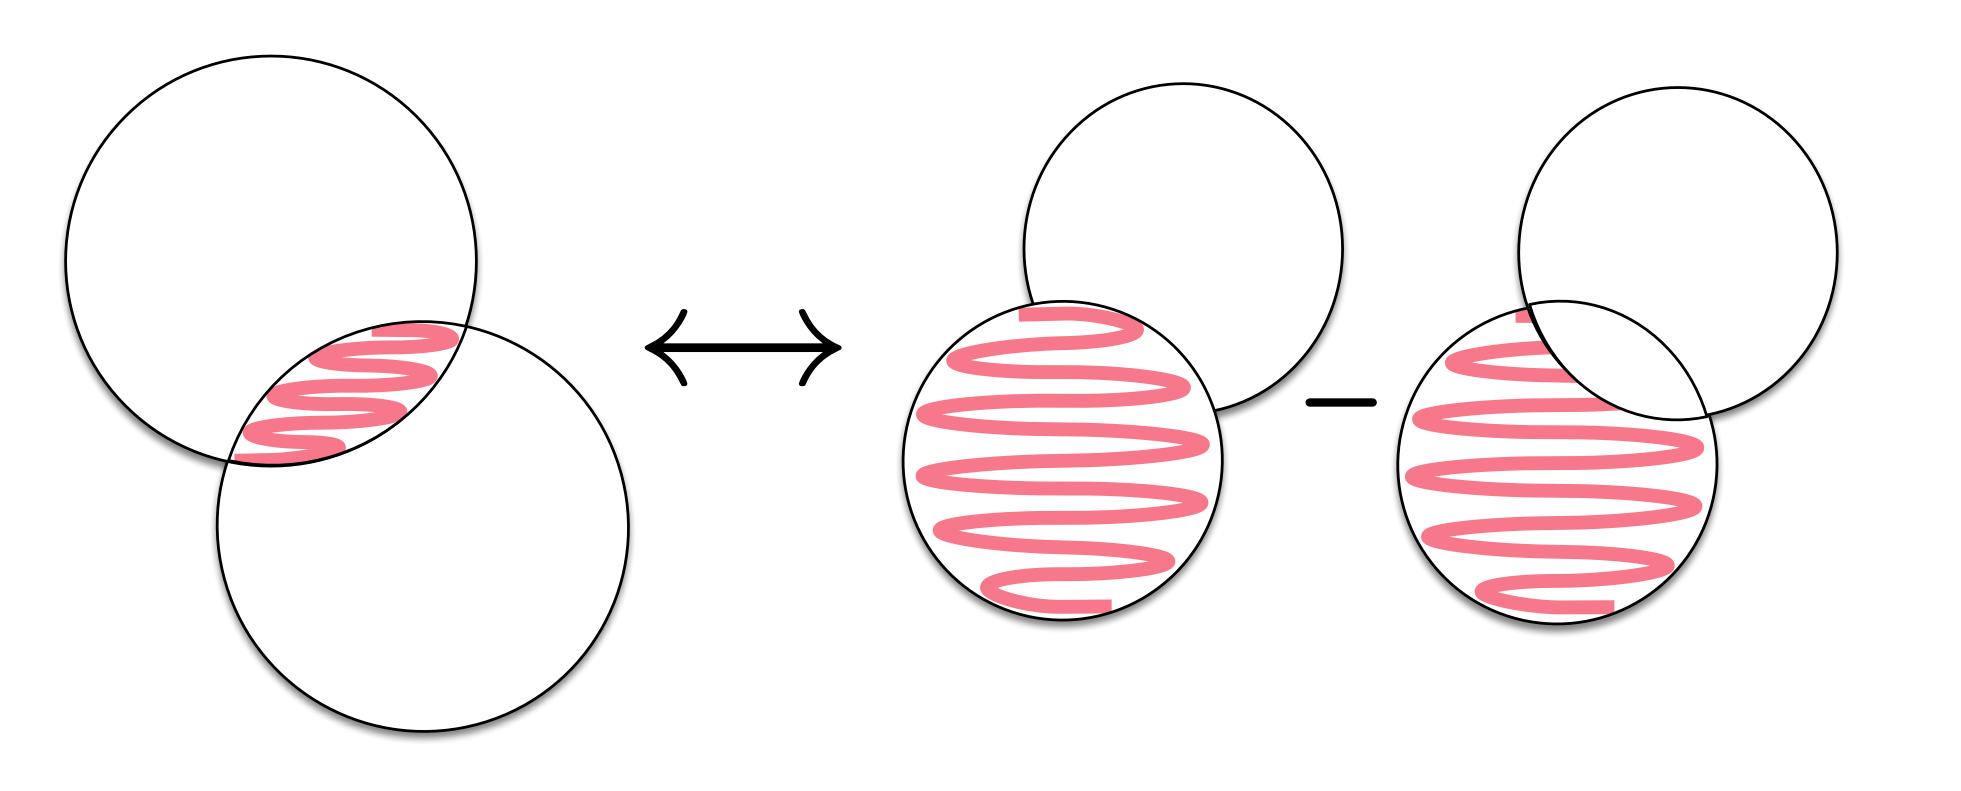
\includegraphics[width=12cm]{images/intersection1.png}
\caption{Venn-Diagram showing the definition of Intersection in terms of Set Difference}
\end{figure}
        
    \vspace{0.1in}
    
     \textbf{Part 4} \\
    Explain the difference between DRC and TRC.
    
    \vspace{0.1in}
        \solution \\
In Tuple Relational Calculus (TRC), the variables typically range over tuples, i.e. they directly represent tuples. On the other hand, in Domain Relational Calculus (DRC), the variables range over domain elements, i.e. field values. In TRC, tuples are semantically equivalent to variables, i.e. field referencing can be used to select tuple parts. On the other hand, in DRC, formal variables are explicit and have to be defined.
    \vspace{0.1in}
    
    
\end{homeworkProblem}   

\begin{homeworkProblem}

\textbf{Part 1} \\

The names of the seas that are deeper than 3000 mt and into which at least one river finally flows.

\vspace{0.1in}
    \solution \\
      
    $<name> \mid \exists depth, rname, river, lake, sea, length, sLong, sLat, mount, sAlt, estLong, estLat \\
    Sea(name, depth) \wedge  \\ River(rname, river, lake, sea, length, sLong, sLat, mount, sAlt, estLong, estLat) \wedge \\ depth > 3000 \wedge sea = name$ 
    \vspace{0.1in}
    
\textbf{Part 2} \\
The names of the groups of islands that consist only of islands that are neither 'volcanic' nor
'coral'.

 \vspace{0.1in}
    \solution \\ \\    
   %SOLUTION
   $<islands> \mid \exists name, area, height, type, long, lat \\
Island(name, islands, area, height, type, long, lat) \wedge \\
type \notin \{volcanic, coral\} \wedge islands \neq \emptyset  $
    \vspace{0.1in}    

\textbf{Part 3} \\
The name of the mountain, the name of the mountains where it belongs to and the name of
the country where the mountain is located for each mountain that is located on an island
that is of type 'coral'.

 
 \vspace{0.1in} 
     \solution \\ \\ 
     %SOLUTION   
     $<moiMountain, mMountains, gmCountry> \mid \exists \\ moiIsland, mHeight, mType, mLong, mLat, \\ iIslands, iArea, iHeight, iType, iLong, iLat, gmProvince \\
mountainOnIsland(moiMountain, moiIsland) \wedge \\ Mountain(moiMountain, mMountains, mHeight, mType, mLong, mLat) \wedge \\ geo\_Mountain(moiMountain, gmCountry, gmProvince)  \wedge \\
Island(moiIsland, iIslands, iArea, iHeight, iType, iLong, iLat) \wedge iType \neq "coral" $

     \vspace{0.1in}

    
\textbf{Part 4} \\
Give the name and country name of all cities with a population higher than 500,000.

 \vspace{0.1in} 
     \solution \\ \\    
    %SOLUTION
   $<cName, coName> \mid \exists cCountry, cProvince, cPopulation, cLong, cLat, \\
   coCapital, coProvince, coArea, coPopulation \\
City(cName, cCountry, cProvince, cPopulation, cLong, cLat)  \wedge \\
Country(cCountry, coName, coCapital, coProvince, coArea, coPopulation) \wedge \\
cPopulation > 500000 $
 
    \vspace{0.1in}
        
\end{homeworkProblem}

\begin{homeworkProblem}
Suppose you have a file of 15,000 pages and eight buffer pages and you are sorting it using general
(external) merge-sort. Please answer the following questions: \\

\textbf{Part 1} \\
How many runs will you produce? Remark: When a file is sorted, in intermediate steps
subfiles are created. Each sorted subfile is called a run. See also slide 35 in Chapter 2.
 \textbf{Note: Detailed solution of Q3 is produced in \textit{Figures 2, 3 and 4.}}
 
 \vspace{0.1in} 
     \solution \\
     %SOLUTION
     \textbf{2189} runs will be produced   
     \vspace{0.1in}
     
 \textbf{Part 2} \\
How many passes will it take to sort the file completely?
 
 \vspace{0.1in} 
     \solution \\ 
    It will take \textbf{5} passes   
     \vspace{0.1in}
     
 \textbf{Part 3} \\
How many buffer pages do you need at least to sort the file in two passes? 

 \vspace{0.1in} 
     \solution \\
     With \textbf{123} buffers, you can sort the file in two passes 
     \vspace{0.1in}
 
 \textbf{Part 4} \\
How many runs and passes would a Two-Way-Sort algorithm take?
 
 \vspace{0.1in} 
     \solution \\
     %SOLUTION
     Two-Way Sort Algorithm will take \textbf{30004} runs and \textbf{15} passes   
     \vspace{0.1in}   
     
\begin{figure}[h]
\centering
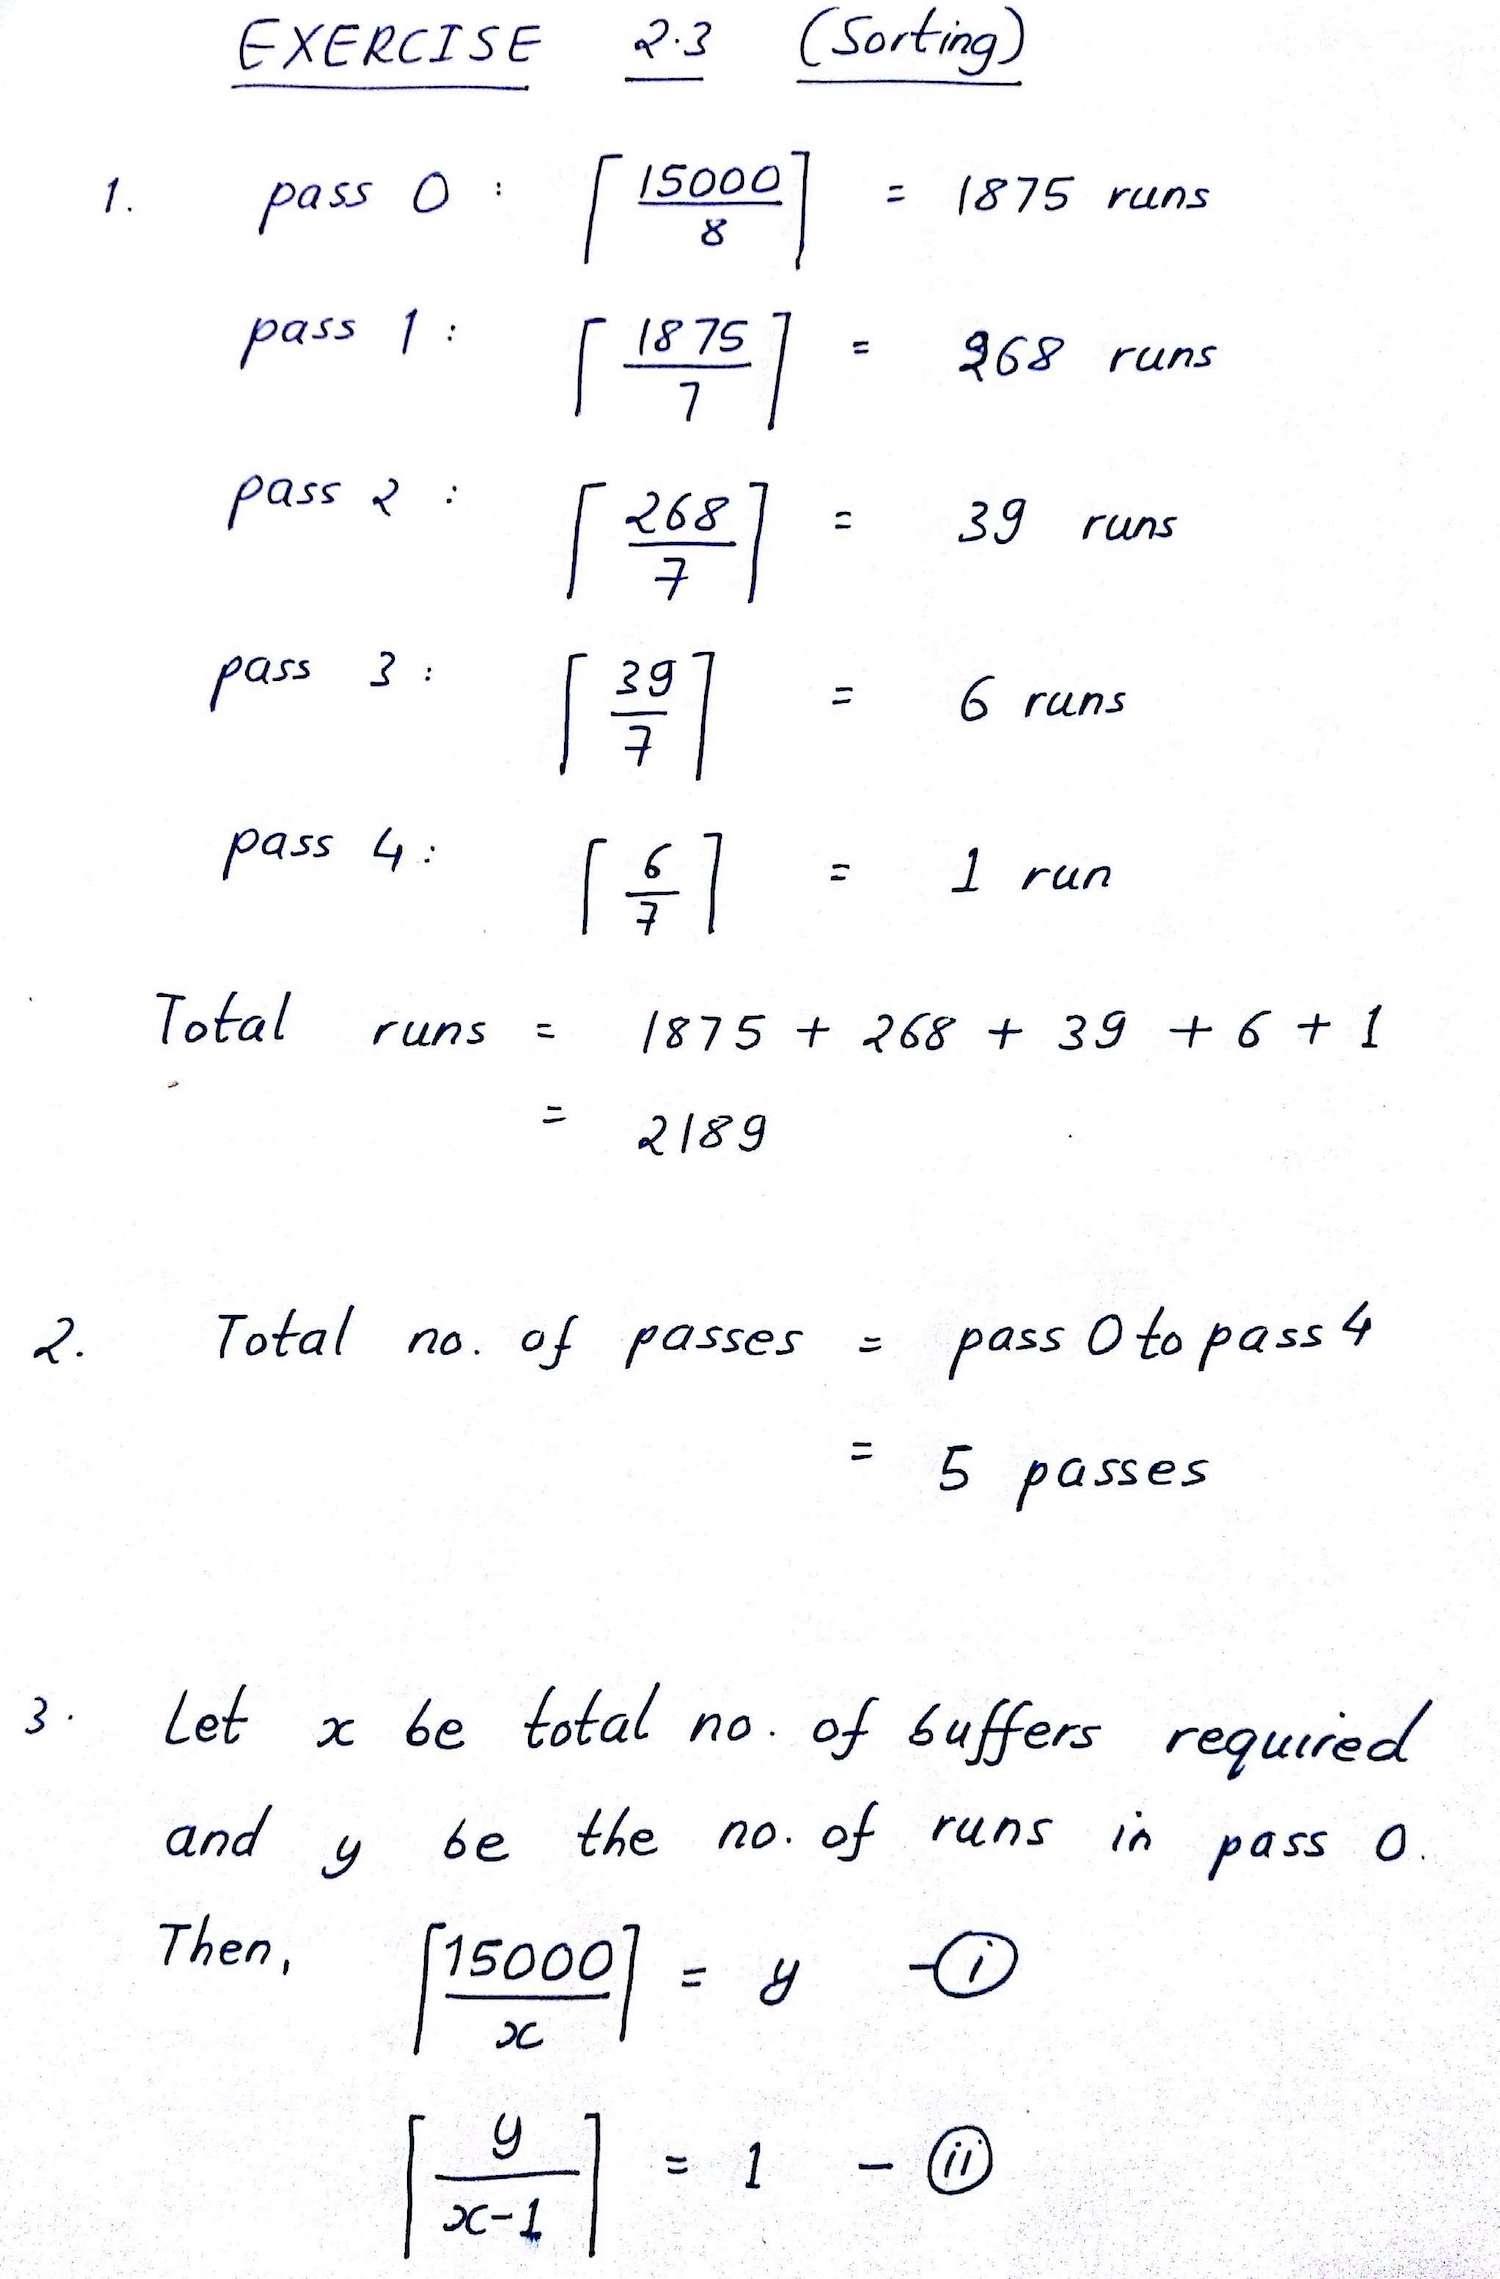
\includegraphics[width=12cm]{images/sol31.jpg}
\caption{Paper-based Solution for Question 3-1}
\end{figure} 

\begin{figure}[h]
\centering
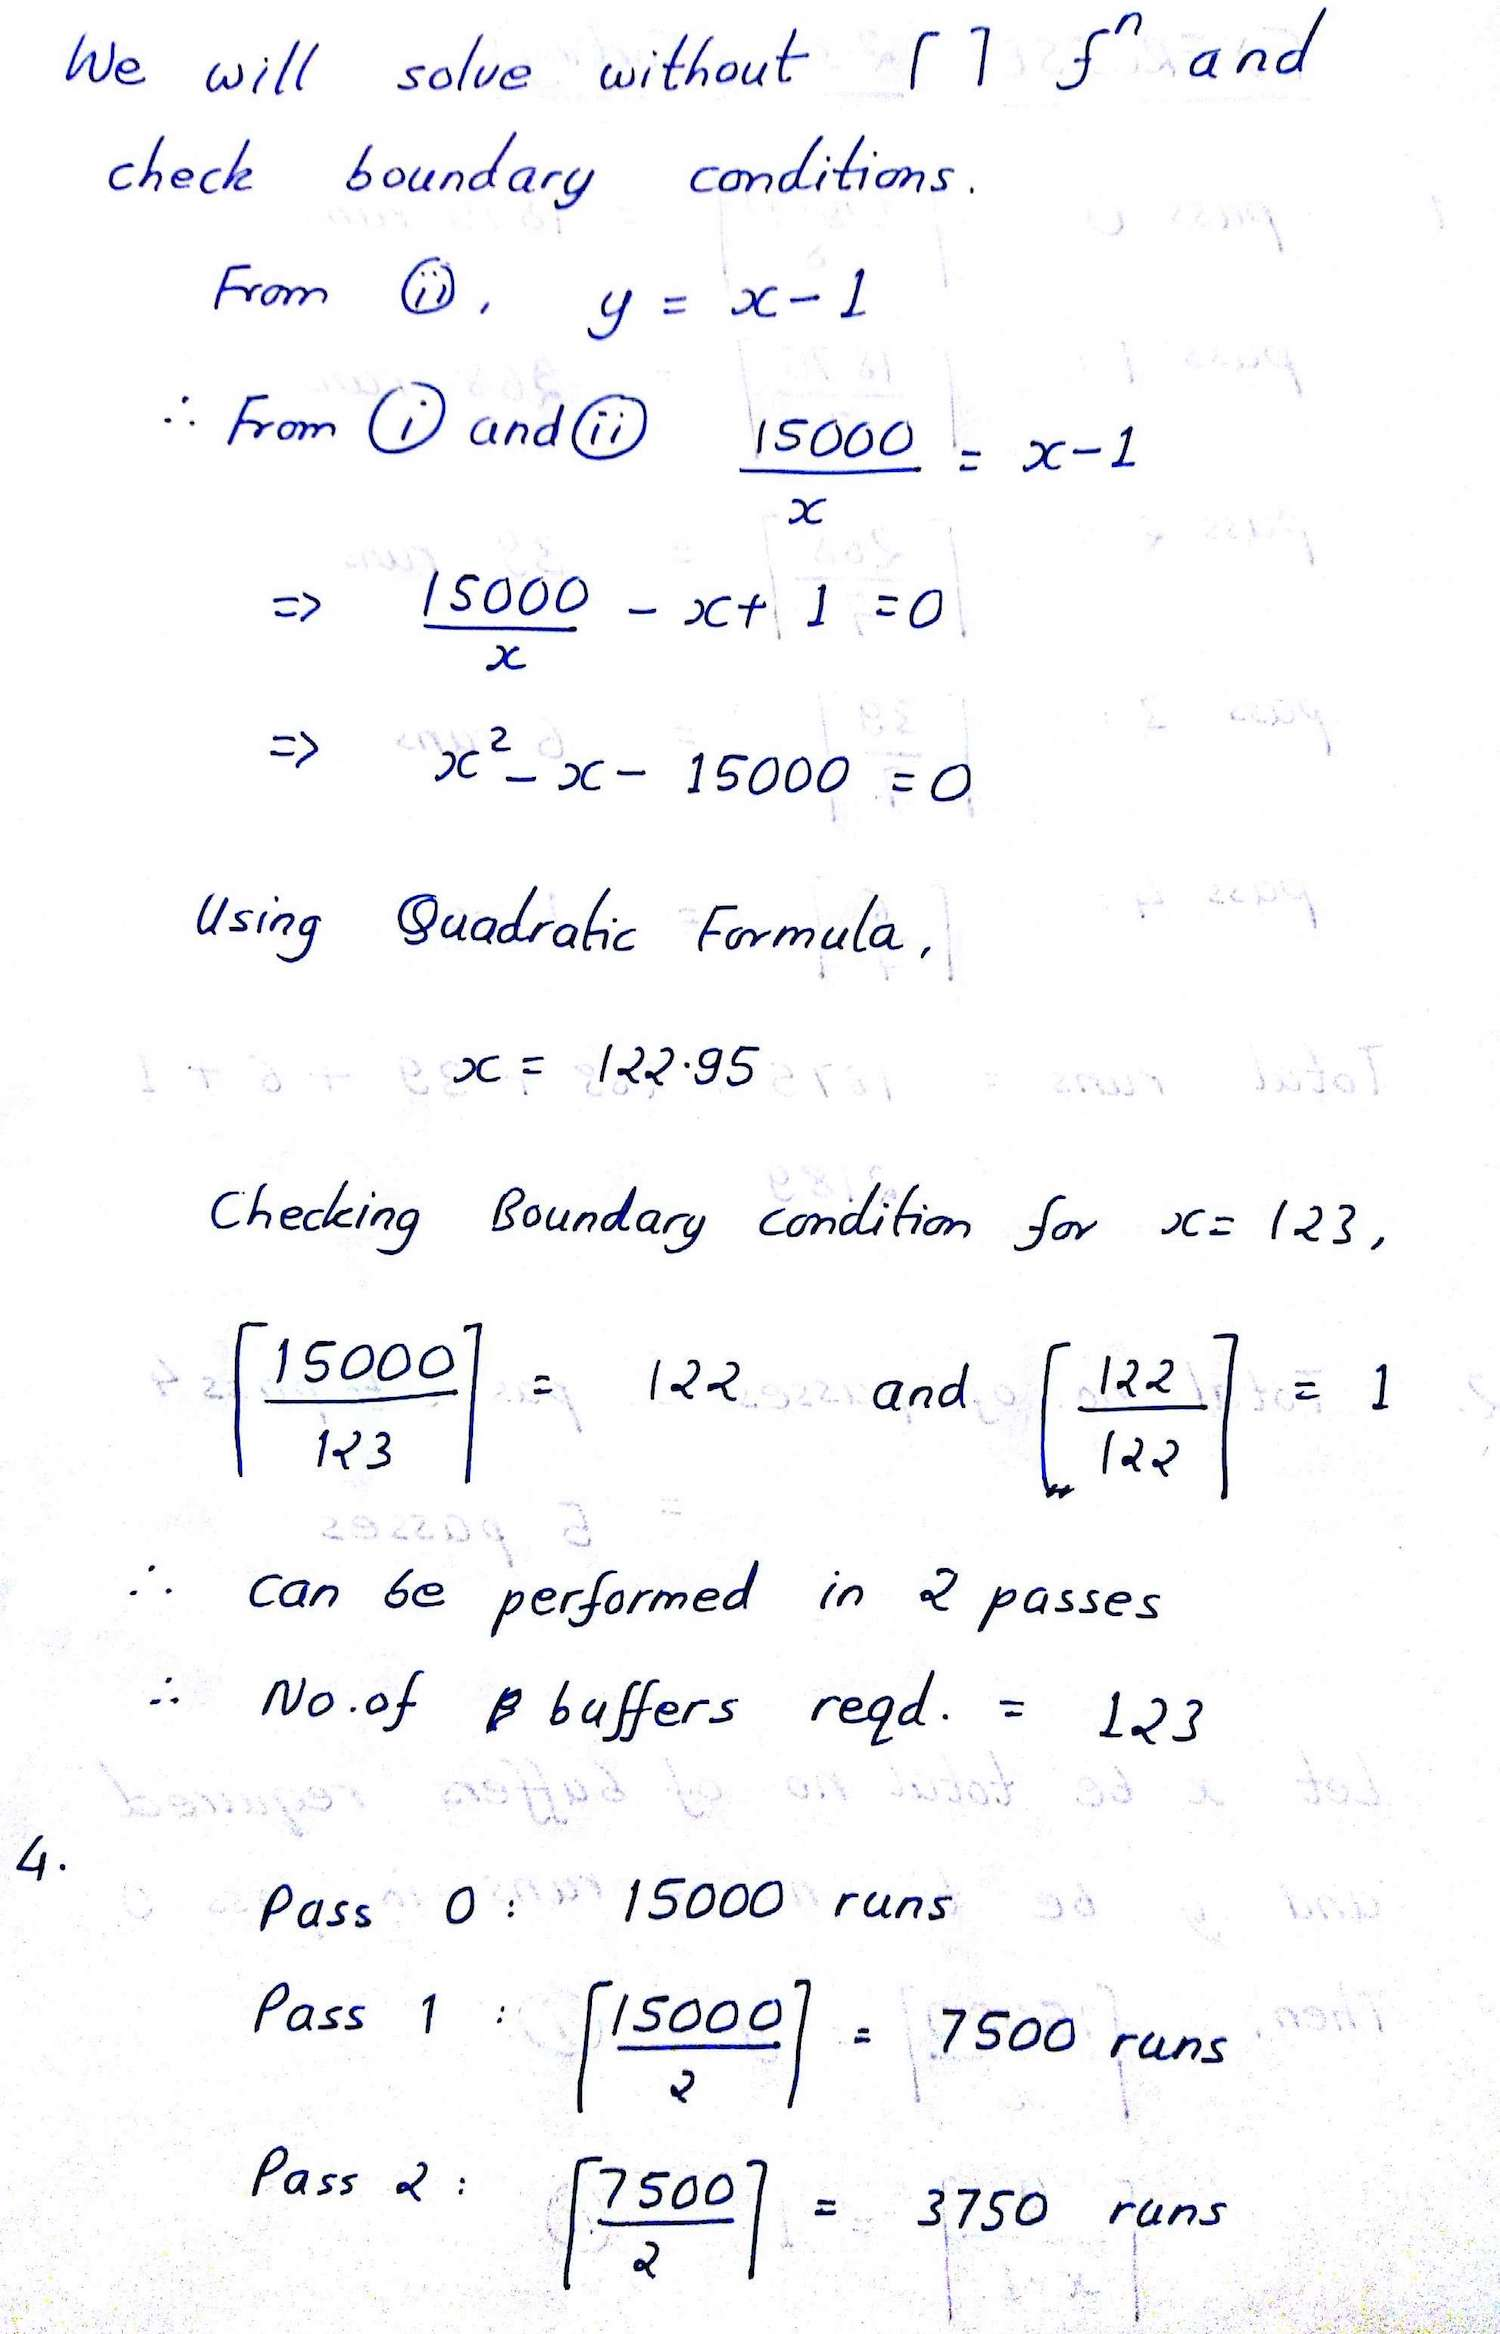
\includegraphics[width=12cm]{images/sol32.jpg}
\caption{Paper-based Solution for Question 3-2}
\end{figure} 

\begin{figure}[h]
\centering
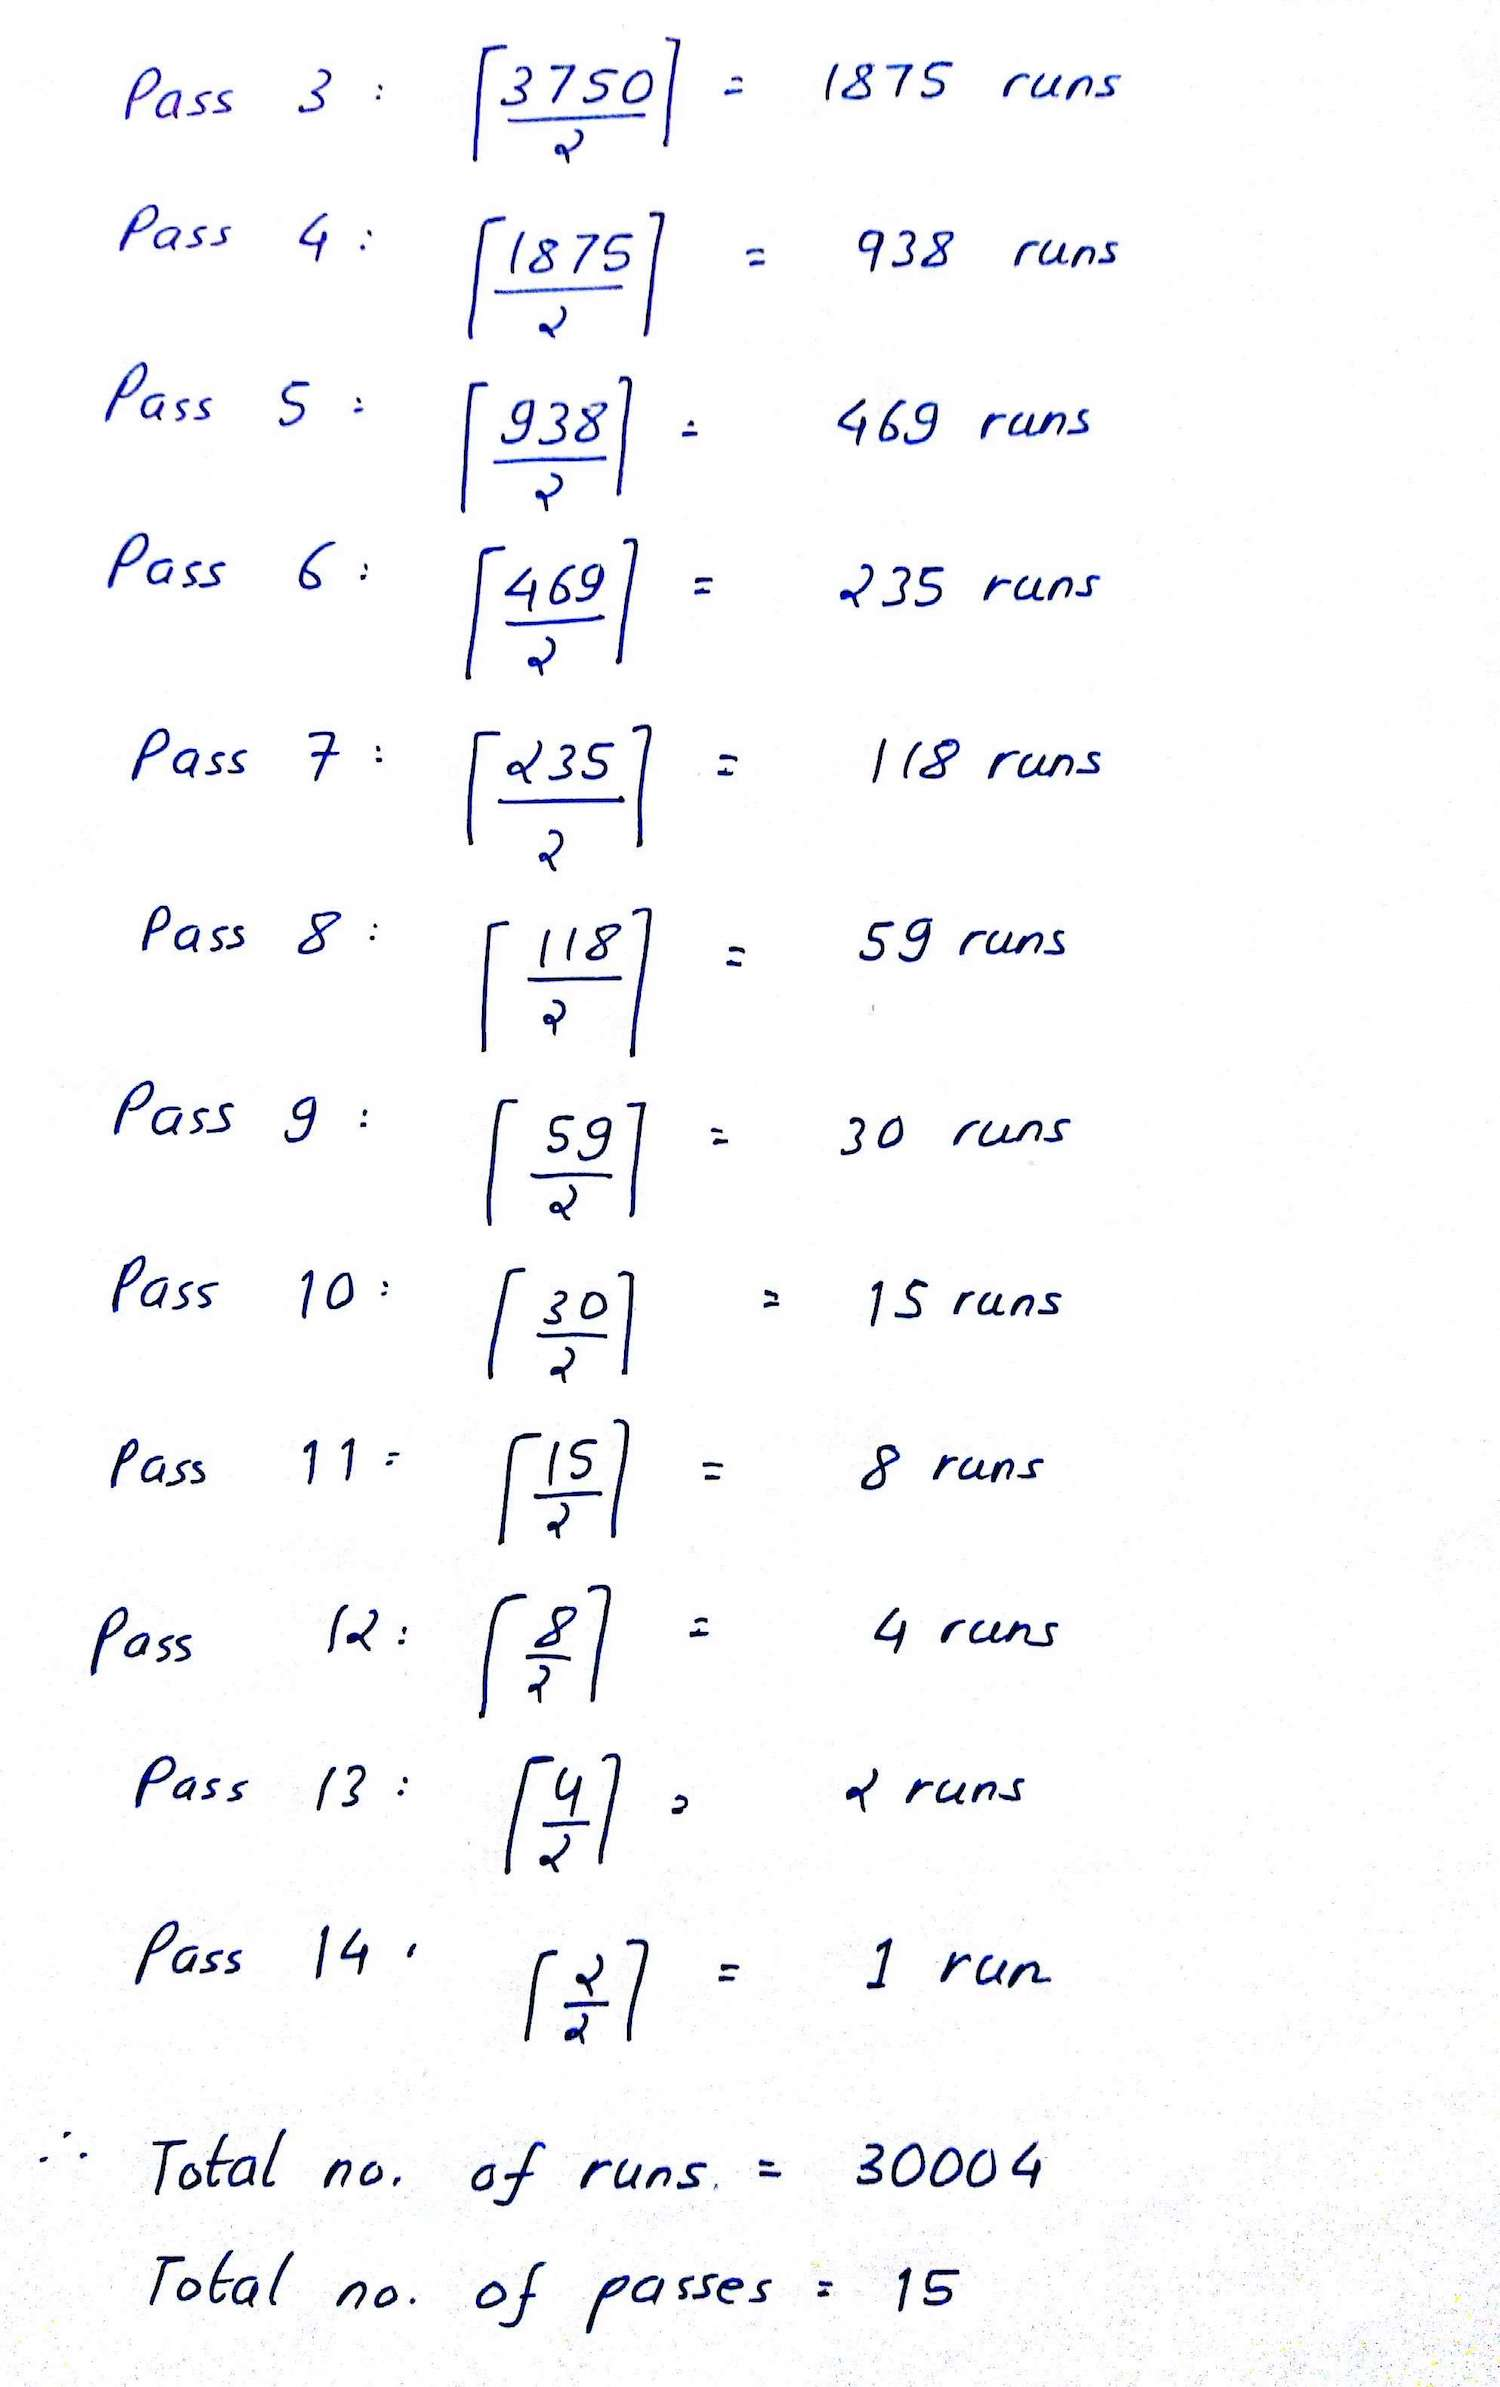
\includegraphics[width=12cm]{images/sol33.jpg}
\caption{Paper-based Solution for Question 3-3}
\end{figure} 

\end{homeworkProblem}

\begin{homeworkProblem}

\textbf{Part 1} \\
Calculate the I/O requirements of a simple nested loop join
 
 \vspace{0.1in} 
     \solution \\ \\ 
     %SOLUTION 
     In the expression below, M and N are the number of pages in the relations Album and Track respectively, $p_M$ and $p_N$ are the number of tuples in each page of the relations. \\
     
     \textbf{M as outer and N as inner relation} \\
     \textbf{Tuple-by-Tuple Simple Nested Loop Join} \\
     $M +  p_M \times M \times N$ \\
     $= 10000 + 100 \times 10000 \times 200000$ \\
     $ = 200000010000 $
          
    \vspace{0.1in}
     \textbf{Page-by-Page Simple Nested Loop Join} \\
     $M + M \times N$ \\
     $= 10000 + 10000 \times 200000$ \\
     $ = 2000010000 $
     
      \vspace{0.1in}
     \textbf{N as outer and M as inner relation} \\
     \textbf{Tuple-by-Tuple Simple Nested Loop Join} \\
     $N +  p_N \times N \times M$ \\
     $= 200000 + 80 \times 200000 \times 10000$ \\
     $ = 160000200000 $
          
    \vspace{0.1in}
     \textbf{Page-by-Page Simple Nested Loop Join} \\
     $M + M \times N$ \\
     $= 200000 + 200000 \times 10000$ \\
     $ = 2000200000 $
     \vspace{0.1in}
     
 \textbf{Part 2} \\
Calculate the I/O requirements of a block nested loop join
 
\vspace{0.1in} 
     \solution \\ \\ 
     %SOLUTION
     Block nested join for 16 buffers: \\
     
      \textbf{M as outer and N as inner relation} \\
     $ 10000 + \lceil \frac{10000}{14} \rceil \times 200000$
     $ = 143010000 $   
     \vspace{0.1in}
     
      \textbf{N as outer and M as inner relation} \\
      $ 200000 + \lceil \frac{200000}{14} \rceil \times 10000$
     $ = 143060000 $   
     \vspace{0.1in}
     
 \textbf{Part 3} \\
Explain the differences between the two algorithms. What are the similarities and differences? How does the block nested loop join reduce I/O costs?
 
 \vspace{0.1in} 
     \solution \\ \\ 
     %SOLUTION
     Tuple-at-a-time Simple Nested Loop Join scans outer relation and then for each tuple, it scans the entire inner relation. On the other hand, the page-at-a-time Simple Nested Loop Join will load the outer relation page-by-page, and then the inner relation for each page. The Block Nested Loop Join, on the other hand, scans entire inner relation for each block of pages in the outer relation. Therefore, the I/O cost of Block Nested Loop Join is lower than cost of both the Simple Nested Loop Joins. 
Moreover, the other important difference is number of buffer pages used in the algorithms. Both tuple-at-a-time nested loop and page-at-time nested loop join use 3 buffer pages to perform the join operation. 1 page as input buffer to scan outer relation,1 page as input buffer to scan inner relation  and 1 page as output buffer. Totally, 3 pages are needed for simple nested loop join. However, block nested loop join uses 1 page as input buffer to scan inner relation S and 1 page as output buffer. The other remaining buffer pages are used to load the blocks of the outer relation R. In this case, 1 buffer page is used as input buffer to scan inner relation  and 1 page as output buffer. Remaining 14 buffer pages are used to block outer relation . As seen, block nested loop join uses entire available buffer pages in the algorithm that means more efficient usage of buffer pages and causing performance increases and decreasing I/O cost. 

The similarities can be indicated as outer-inner relation usage, buffer usage and loop operations in the algorithms. 

     \vspace{0.1in}
     
\end{homeworkProblem}
     
\begin{homeworkProblem}
Given is a relation with 50.000 records. Each page for a node in a B+ tree can hold 20 pointers
to records or pages. A data page can store 20 records. \\

 \textbf{Part 1} \\
Assume that each node is 70 \% full. What is the height of the B+-tree? 

 \vspace{0.1in} 
     \solution \\ \\ 
     %SOLUTION  
     Given that the B+Tree can hold 20 pointers to pages. However, the B+ Tree has 70\% occupancy. Therefore, number of effective pointers to pages that the tree can hold,
     \begin{center} $ \implies 0.7 \times 20 = 14$ \end{center} 
Our B+ Tree can now be represented as Table 1

\begin{table}[]
\centering
\begin{tabular}{|l|l|l|l|}
\hline
Level    & Node & Entries & No. of Pointers \\ \hline
0 (Root) & 1    & 13      & 14              \\ \hline
1        & 14   & 182     & 196             \\ \hline
2        & 196  & 2548    & 2744         \\ \hline  
\end{tabular}
\caption{Different Levels of the B+ Tree}
\label{B+ Tree}
\end{table}

We have 2744 addresses in Level 2 already, which is more than 2500 pointers to pages required in the relations. \\
Therefore, the B-Tree has a depth of \textbf{3}.
Our B+ Tree has a depth of \textbf{3}
 \vspace{0.1in}
     
 \textbf{Part 2} \\
What are the I/O costs for an equality selection on a non-key attribute for the following
cases?

\begin{enumerate}[label = (\alph*)]
\item with a clustered B+-tree of height 3 (matching records are located in one page);
 
 \vspace{0.1in} 
     \solution \\ \\ 
     %SOLUTION
     The clustered index will guide the search, and after the end of the B+ tree traversal, we will need to input the correct page which contains our desired result. Therefore, total I/O is for the tree traversal and retrieving the correct page, i.e. 3 I/Os + 1 I/O = 4.
     Hence, total number of I/Os = \textbf{4} I/Os
     \vspace{0.1in}
     
\item without any index, nor is the file sorted on the attribute occurring in selection;

\vspace{0.1in} 
     \solution \\ \\ 
     %SOLUTION 
     Total number of pages at the leaf node = 2500
    If we consider that all pages need to be scanned, then the I/O costs will be \textbf{2500} I/Os. \\
    However, assuming, on an average that half the total number of pages need to be searched to find the equality results, it gives a total of 1250 I/Os.
          
     \vspace{0.1in}
     
\item with an unclustered B+-tree index of height 4, and there are 2 matching records;

\vspace{0.1in} 
     \solution \\ \\ 
     4 I/Os to traverse the tree + 2 I/Os to retrieve the matching records = \textbf{6} I/Os 
     \vspace{0.1in}

\item with an unclustered B+-tree of height 5 and three tenth of the records match the
selection.

\vspace{0.1in} 
\solution \\ \\ 
     %SOLUTION
     No. of matching records = $\frac{3}{10} \times 50000 = 15000$ records \\
     In the worst case, we need to do 15000 page I/Os, one for each record. Plus the I/Os for traversing the tree. Therefore, a total of 15000 I/Os + 5 I/Os = \textbf{15005} I/Os.   
     \vspace{0.1in}

\end{enumerate}
\end{homeworkProblem}

\end{document}
\documentclass[12pt]{article}

\usepackage{fancyhdr}
\usepackage{extramarks}
\usepackage{amsmath}
\usepackage{amsthm}
\usepackage{amsfonts}
\usepackage{tikz}
\usepackage[plain]{algorithm}
\usepackage{algpseudocode}
\usepackage[export]{adjustbox}
\usepackage[latin1]{inputenc}           %For German characters
\usepackage{enumitem}               %For changing enumeration character
\usepackage{listings}               %For code
\usepackage{csquotes}
\usepackage{graphicx}               %For graphics e.g, images

\usetikzlibrary{automata,positioning}

%
% Basic Document Settings
%

\topmargin=-0.45in
\evensidemargin=0in
\oddsidemargin=0in
\textwidth=6.5in
\textheight=9.0in
\headsep=0.25in

\linespread{1.1}

\pagestyle{fancy}
\lhead{\hmwkAuthorName}
\chead{\hmwkClass\ : \hmwkTitle}
\rhead{\firstxmark}
\lfoot{\lastxmark}
\cfoot{\thepage}

\renewcommand\headrulewidth{0.4pt}
\renewcommand\footrulewidth{0.4pt}

\setlength\parindent{0pt}

%
% Create Problem Sections
%

\newcommand{\enterProblemHeader}[1]{
    \nobreak\extramarks{}{Problem \arabic{#1} continued on next page\ldots}\nobreak{}
    \nobreak\extramarks{Problem \arabic{#1} (continued)}{Problem \arabic{#1} continued on next page\ldots}\nobreak{}
}

\newcommand{\exitProblemHeader}[1]{
    \nobreak\extramarks{Problem \arabic{#1} (continued)}{Problem \arabic{#1} continued on next page\ldots}\nobreak{}
    \stepcounter{#1}
    \nobreak\extramarks{Problem \arabic{#1}}{}\nobreak{}
}

\setcounter{secnumdepth}{0}
\newcounter{partCounter}
\newcounter{homeworkProblemCounter}
\setcounter{homeworkProblemCounter}{1}
\nobreak\extramarks{Problem \arabic{homeworkProblemCounter}}{}\nobreak{}

%
% Homework Problem Environment
%
% This environment takes an optional argument. When given, it will adjust the
% problem counter. This is useful for when the problems given for your
% assignment aren't sequential. See the last 3 problems of this template for an
% example.
%
\newenvironment{homeworkProblem}[1][-1]{
    \ifnum#1>0
        \setcounter{homeworkProblemCounter}{#1}
    \fi
    \section{Problem \arabic{homeworkProblemCounter}}
    \setcounter{partCounter}{1}
    \enterProblemHeader{homeworkProblemCounter}
}{
    \exitProblemHeader{homeworkProblemCounter}
}

%
% Homework Details
%   - Title
%   - Due date
%   - Class
%   - Section/Time
%   - Instructor
%   - Author
%

\newcommand{\hmwkTitle}{Assignment\ \#2}
\newcommand{\hmwkDueDate}{November 15, 2016}
\newcommand{\hmwkClass}{Implementation of Databases}
\newcommand{\hmwkAuthorName}{Sanchit Alekh}
\newcommand{\hmwkClassTime}{MSc. Software Systems Engineering}
\newcommand{\hmwkClassInstructor}{Universitätsprofessor Dr. rer. pol. Matthias Jarke}
\newcommand{\hmwkClassInstructors}{Dr. rer. nat. Christoph Quix}

%
% Title Page
%



\title{
   \begin{center}
   \vspace*{-20mm}
   
\includegraphics[width=0.4\textwidth, right]{images/rwth_logo.png}
   \\
   \vspace*{3cm}
    \textmd{\textbf{\hmwkClass}}\\
    \textmd{\textbf{\hmwkTitle}}\\
    \normalsize\vspace{0.1in}\small{Due\ on\ \hmwkDueDate } \\
    \vspace{0.1in}\large{\textit{\hmwkClassInstructor}} \\
    \vspace{0.1in}\large{\textit{\hmwkClassInstructors}} \\
    \vspace{3in}
     \textbf{Submitted by:} \\
     \vspace{0.25in}
    \large{Sanchit Alekh, Idil Esen Zülfikar, Nihal Hegde} \\
    %\author{\textbf{\hmwkAuthorName}}
    \vspace{0.1in} \large{\textit{\hmwkClassTime}} \\
    %\vspace{0.1in} \large{\textit{Matrikelnummer : 359831}}
    \end{center}
    }


\date{}

\renewcommand{\part}[1]{\textbf{\large Part \Alph{partCounter}}\stepcounter{partCounter}\\}

%
% Various Helper Commands
%

% Useful for algorithms
\newcommand{\alg}[1]{\textsc{\bfseries \footnotesize #1}}

% For derivatives
\newcommand{\deriv}[1]{\frac{\mathrm{d}}{\mathrm{d}x} (#1)}

% For partial derivatives
\newcommand{\pderiv}[2]{\frac{\partial}{\partial #1} (#2)}

% Integral dx
\newcommand{\dx}{\mathrm{d}x}

% Alias for the Solution section header
\newcommand{\solution}{\textbf{\large Solution}}

% Probability commands: Expectation, Variance, Covariance, Bias
\newcommand{\E}{\mathrm{E}}
\newcommand{\Var}{\mathrm{Var}}
\newcommand{\Cov}{\mathrm{Cov}}
\newcommand{\Bias}{\mathrm{Bias}}

\begin{document}

\maketitle

\pagebreak

\begin{homeworkProblem}
    
    \textbf{Part 1} \\
    Variants of relational algebra are used internally in DBMS to represent queries and query evaluation plans. Please explain, why relational algebra is suitable for this?
    
    \vspace{0.1in}
    \solution \\
    One of the most desirable properties of Relational Algebra is that queries are composed using a collection of operators, and every operator accepts one or two relation instances as arguments and returns a relation instance as the result. This property makes extremely easy and efficient to compose operators to form a complex query. A relational algebra expression can be recursively defined to be a relation, a unary algebra operator applied to a single expression, or a binary algebra operator applied to two expressions. 
This procedural nature of relational algebra is the main reason why it is used internally in DBMS to represent queries and evaluation plans. The approach allows us to think of an algebra expression as an imperative execution plan for a declarative SQL query. It can be used for evaluating a query, and relational systems in fact use algebra expressions to represent query evaluation plans.
        
    \vspace{0.1in}
    
    \textbf{Part 2} \\
    What does \enquote{relational completeness} mean (in your own words, please)? Show that SQL is
relationally complete by enumerating SQL constructs corresponding to selection, projection,
cartesian product, union, and difference.
    
    \vspace{0.1in}
    \solution \\
    \enquote{Relational Completeness} of a query methodology means that each and every query that can be expressed using that methodology, can also be expressed as a relational algebra query. In this case, SQL is referred to as \enquote*{Relationally Complete} because every legal construct in SQL can be expressed as a Relational Algebra query.
        
These are the examples of Relational Algebra expressions and their equivalent expressions in SQL. The following examples are derived from the \textit{Mondial} database.

\begin{itemize}

\item \textbf{SELECTION} \\
Relational Algebra: $ \sigma_{Area > 650} (Island)$ \\
SQL:  \textit{Select * From Island Where Area $>$ 650;}

\item \textbf{PROJECTION} \\
Relational Algebra: $ \pi_{Name, Islands, Area, Height} (Island)$ \\
SQL: \textit{Select Name, Islands, Area, Height From Island;}

\item \textbf{CARTESIAN PRODUCT} \\
Relational Algebra:  $ Island \times islandIn$ \\
SQL: \textit{Select * From Island CROSS JOIN islandIn;}

\item \textbf{UNION} \\
Relational Algebra:  $ \pi_{name} (Desert) \cup \pi_{name} (geo\_Desert)$ \\
SQL: \textit{Select name From Desert or Select name From geo\_Desert}

\item \textbf{SET DIFFERENCE} \\
Relational Algebra: $ \pi_{name} (\sigma_{height > 5000} (Mountain)) - \pi_{name}( \sigma_{type > 'volcanic')} (Mountain) $ \\
SQL: \textit{Select name From Mountain where height $>$ 5000 MINUS Select name From Mountain where type='volcanic'}
\end{itemize}
        
    \vspace{0.1in}
        
     \textbf{Part 3} \\
    Explain how the intersection operator is used in relational algebra. What is important for
its usage? Is it omittable (i.e., could you express it by other operators)? If so, please give
the corresponding relational algebra.
    
    \vspace{0.1in}
    \solution \\
    The \enquote*{Intersection} operator is represented in Relational Algebra with the help of the $\cap$ symbol. Although it is not a fundamental set-operator, it is an extremely widely used operation, and it is helpful to define it separately. An example use of the intersection operator is as follows:
    
    \begin{center} $ \pi_{name} (Desert) \cap \pi_{name} (geo\_Desert) $ \end{center}
    
The important condition for using the \textit{Intersection} operator is that the two sets which have to be intersected must be \textit{union-compatible}. This follows from the fact that intersection is defined in terms of set difference.

Yes, Intersection is not a fundamental set-operator, and it can be expressed in terms of the set-difference operator. Therefore, it is omittable. A general expression for the intersection operator in terms of the set-difference operator is:

    \begin{center} $ A \cup B \leftrightarrow A \setminus ( A \setminus B) $ \end{center}
    
Therefore, the example Relational Algebra query illustrated above can be represented by the equivalent query without the use of set-intersection as follows:

    \begin{center} $ \pi_{name} (Desert) - (\pi_{name} (Desert) - \pi_{name} (geo\_Desert))$ \end{center}
    
\begin{figure}[h]
\centering
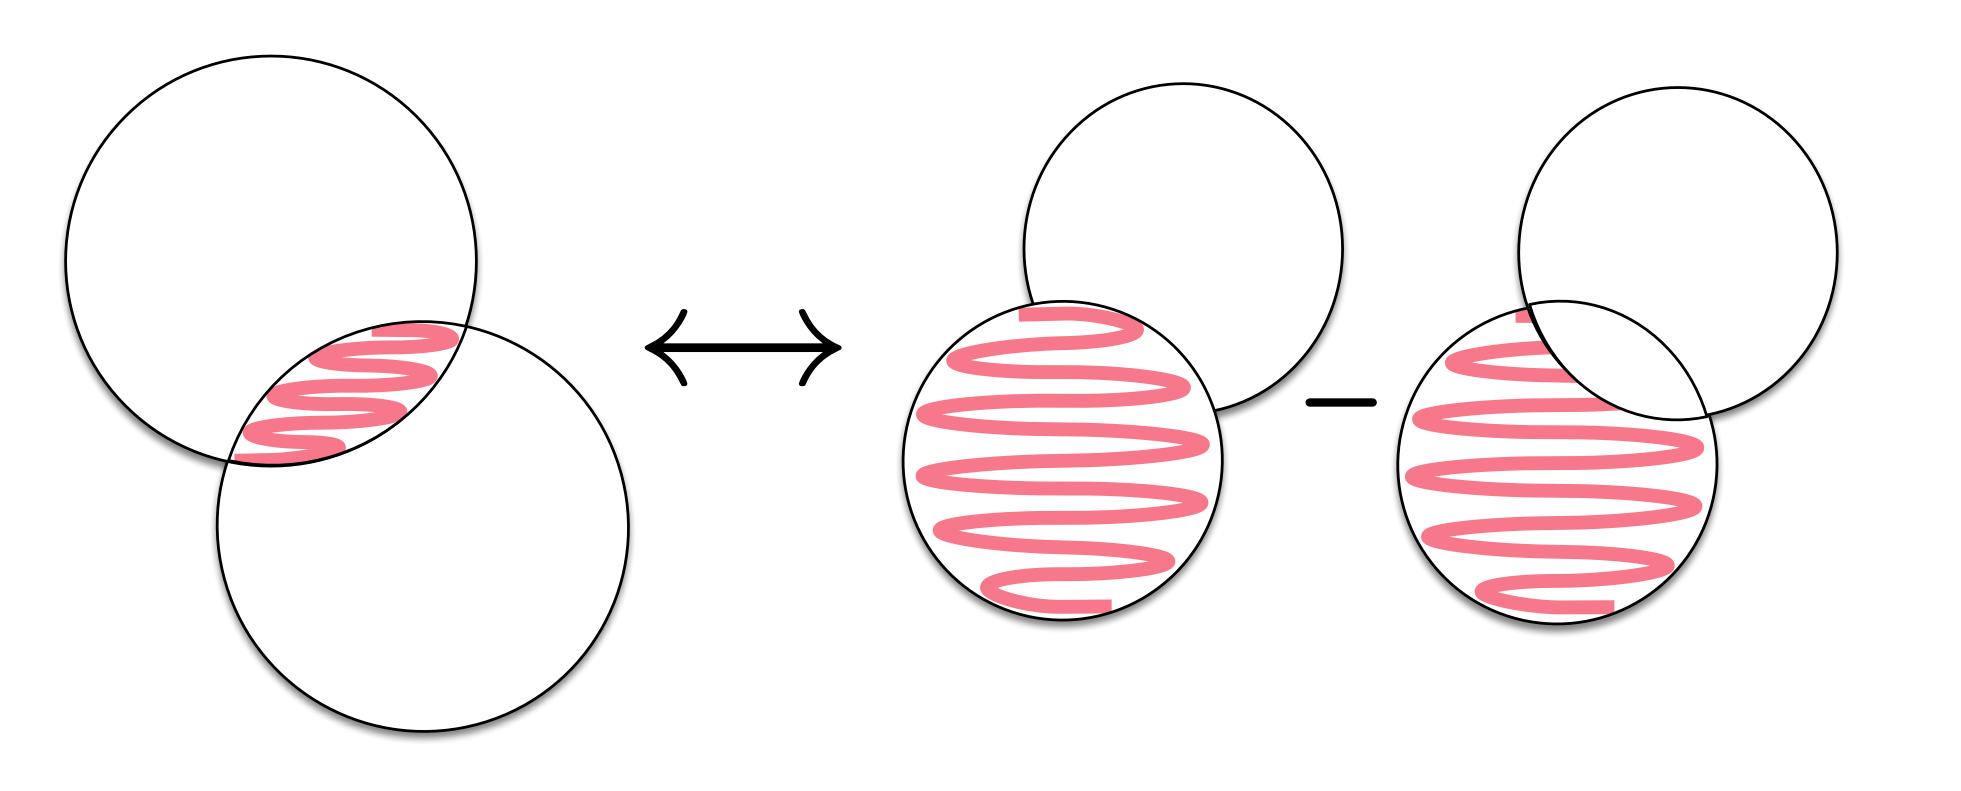
\includegraphics[width=12cm]{images/intersection1.png}
\caption{Venn-Diagram showing the definition of Intersection in terms of Set Difference}
\end{figure}
        
    \vspace{0.1in}
    
     \textbf{Part 4} \\
    Explain the difference between DRC and TRC.
    
    \vspace{0.1in}
        \solution \\
In Tuple Relational Calculus (TRC), the variables typically range over tuples, i.e. they directly represent tuples. On the other hand, in Domain Relational Calculus (DRC), the variables range over domain elements, i.e. field values. In TRC, tuples are semantically equivalent to variables, i.e. field referencing can be used to select tuple parts. On the other hand, in DRC, formal variables are explicit and have to be defined.
    \vspace{0.1in}
    
    
\end{homeworkProblem}   

\begin{homeworkProblem}

\textbf{Part 1} \\

The names of the seas that are deeper than 3000 mt and into which at least one river finally flows.

\vspace{0.1in}
    \solution \\
      
    $<name> \mid \exists depth, rname, river, lake, sea, length, sLong, sLat, mount, sAlt, estLong, estLat \\
    Sea(name, depth) \wedge  \\ River(rname, river, lake, sea, length, sLong, sLat, mount, sAlt, estLong, estLat) \wedge \\ depth > 3000 \wedge sea = name$ 
    \vspace{0.1in}
    
\textbf{Part 2} \\
The names of the groups of islands that consist only of islands that are neither 'volcanic' nor
'coral'.

 \vspace{0.1in}
    \solution \\ \\    
   %SOLUTION
   $<islands> \mid \exists name, area, height, type, long, lat \\
Island(name, islands, area, height, type, long, lat) \wedge \\
type \notin \{volcanic, coral\} \wedge islands \neq \emptyset  $
    \vspace{0.1in}    

\textbf{Part 3} \\
The name of the mountain, the name of the mountains where it belongs to and the name of
the country where the mountain is located for each mountain that is located on an island
that is of type 'coral'.

 
 \vspace{0.1in} 
     \solution \\ \\ 
     %SOLUTION   
     $<moiMountain, mMountains, gmCountry> \mid \exists \\ moiIsland, mHeight, mType, mLong, mLat, \\ iIslands, iArea, iHeight, iType, iLong, iLat, gmProvince \\
mountainOnIsland(moiMountain, moiIsland) \wedge \\ Mountain(moiMountain, mMountains, mHeight, mType, mLong, mLat) \wedge \\ geo\_Mountain(moiMountain, gmCountry, gmProvince)  \wedge \\
Island(moiIsland, iIslands, iArea, iHeight, iType, iLong, iLat) \wedge iType \neq "coral" $

     \vspace{0.1in}

    
\textbf{Part 4} \\
Give the name and country name of all cities with a population higher than 500,000.

 \vspace{0.1in} 
     \solution \\ \\    
    %SOLUTION
   $<cName, coName> \mid \exists cCountry, cProvince, cPopulation, cLong, cLat, \\
   coCapital, coProvince, coArea, coPopulation \\
City(cName, cCountry, cProvince, cPopulation, cLong, cLat)  \wedge \\
Country(cCountry, coName, coCapital, coProvince, coArea, coPopulation) \wedge \\
cPopulation > 500000 $
 
    \vspace{0.1in}
        
\end{homeworkProblem}

\begin{homeworkProblem}
Suppose you have a file of 15,000 pages and eight buffer pages and you are sorting it using general
(external) merge-sort. Please answer the following questions: \\

\textbf{Part 1} \\
How many runs will you produce? Remark: When a file is sorted, in intermediate steps
subfiles are created. Each sorted subfile is called a run. See also slide 35 in Chapter 2.
 \textbf{Note: Detailed solution of Q3 is produced in \textit{Figures 2, 3 and 4.}}
 
 \vspace{0.1in} 
     \solution \\
     %SOLUTION
     \textbf{2189} runs will be produced   
     \vspace{0.1in}
     
 \textbf{Part 2} \\
How many passes will it take to sort the file completely?
 
 \vspace{0.1in} 
     \solution \\ 
    It will take \textbf{5} passes   
     \vspace{0.1in}
     
 \textbf{Part 3} \\
How many buffer pages do you need at least to sort the file in two passes? 

 \vspace{0.1in} 
     \solution \\
     With \textbf{123} buffers, you can sort the file in two passes 
     \vspace{0.1in}
 
 \textbf{Part 4} \\
How many runs and passes would a Two-Way-Sort algorithm take?
 
 \vspace{0.1in} 
     \solution \\
     %SOLUTION
     Two-Way Sort Algorithm will take \textbf{30004} runs and \textbf{15} passes   
     \vspace{0.1in}   
     
\begin{figure}[h]
\centering
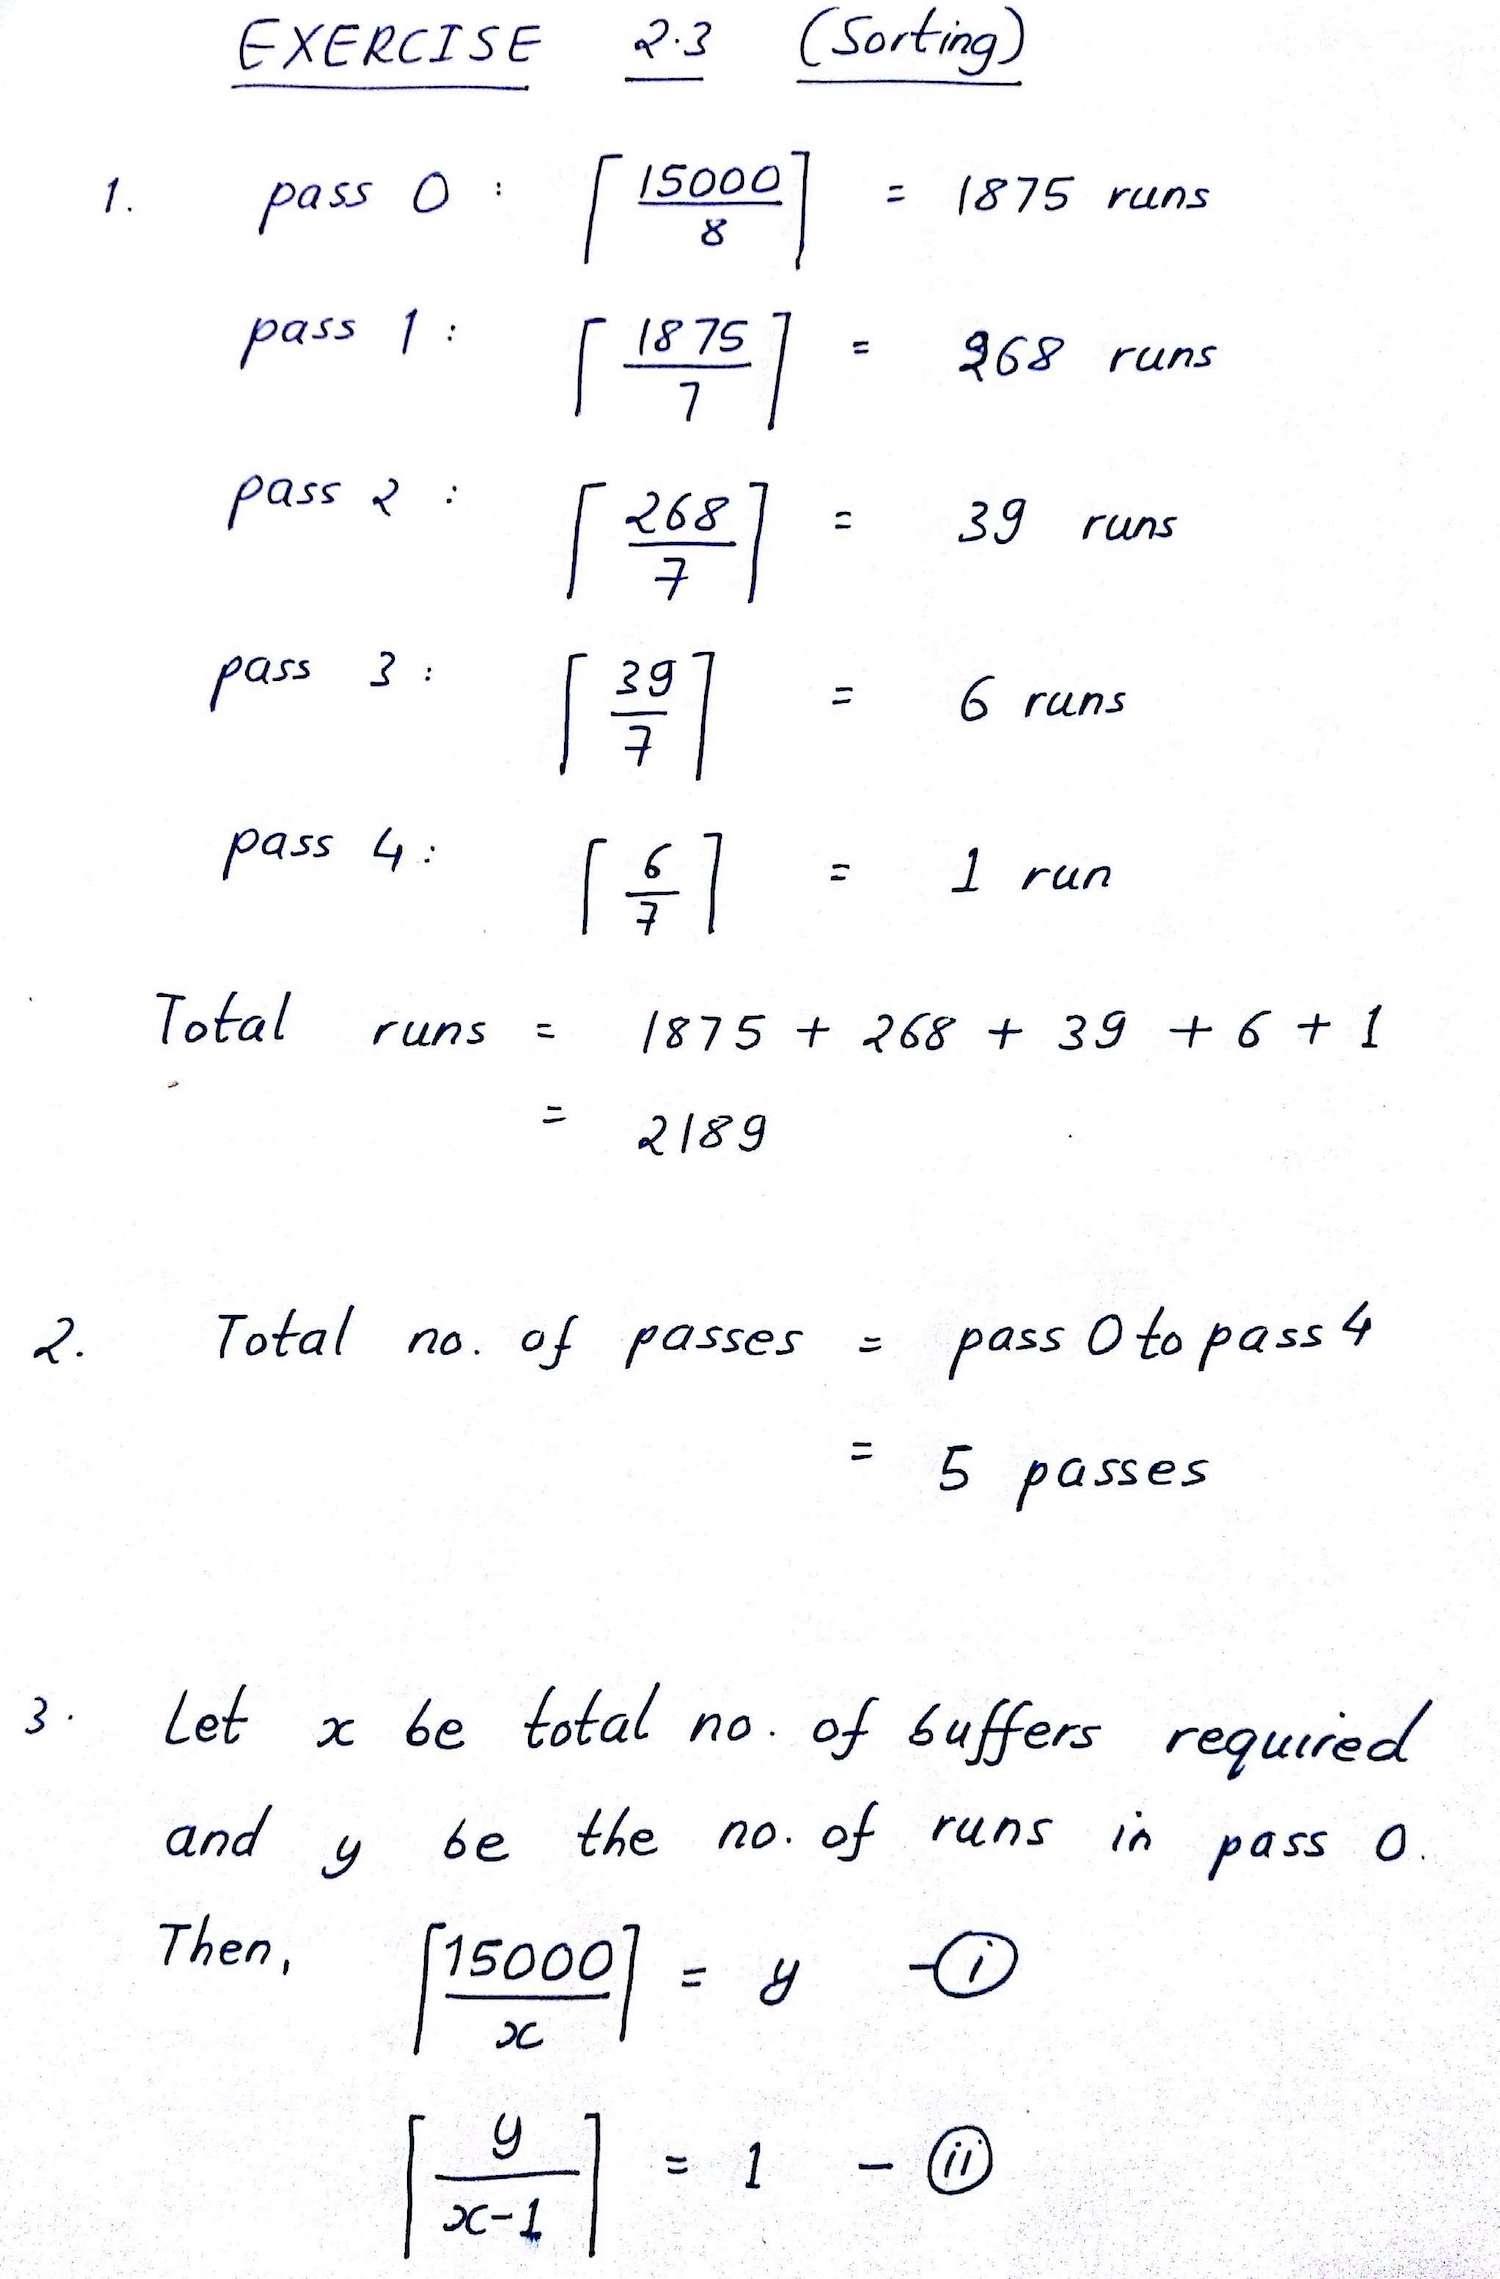
\includegraphics[width=12cm]{images/sol31.jpg}
\caption{Paper-based Solution for Question 3-1}
\end{figure} 

\begin{figure}[h]
\centering
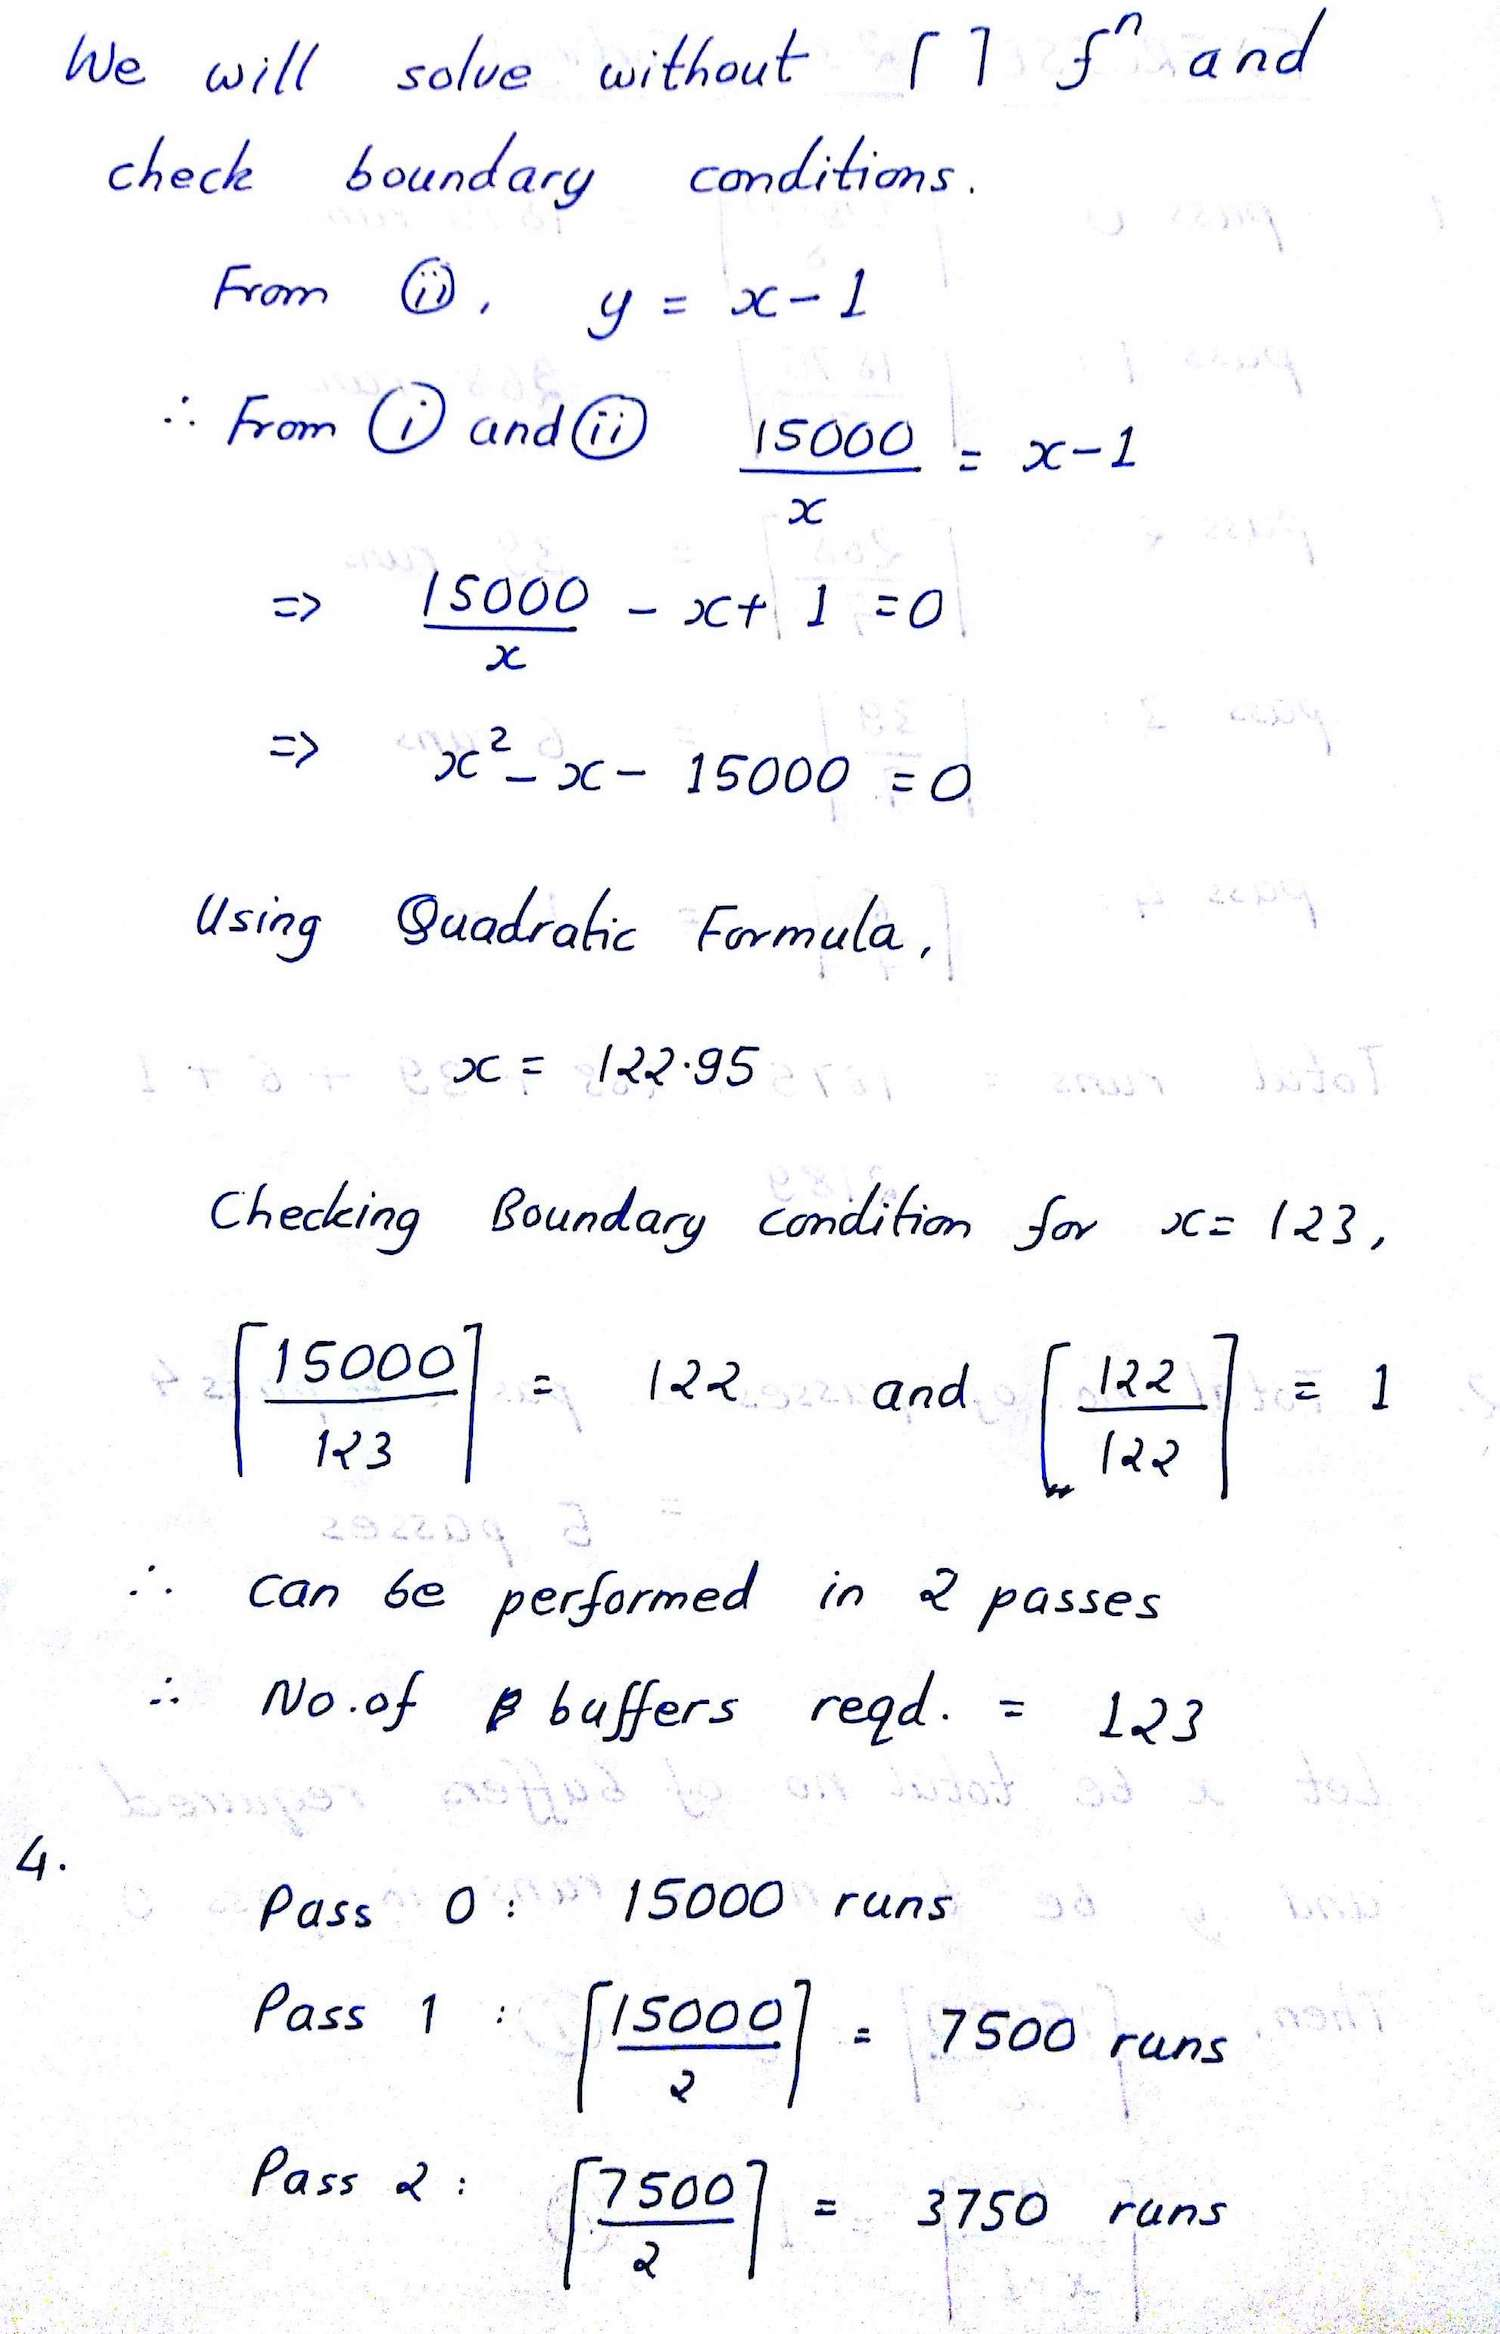
\includegraphics[width=12cm]{images/sol32.jpg}
\caption{Paper-based Solution for Question 3-2}
\end{figure} 

\begin{figure}[h]
\centering
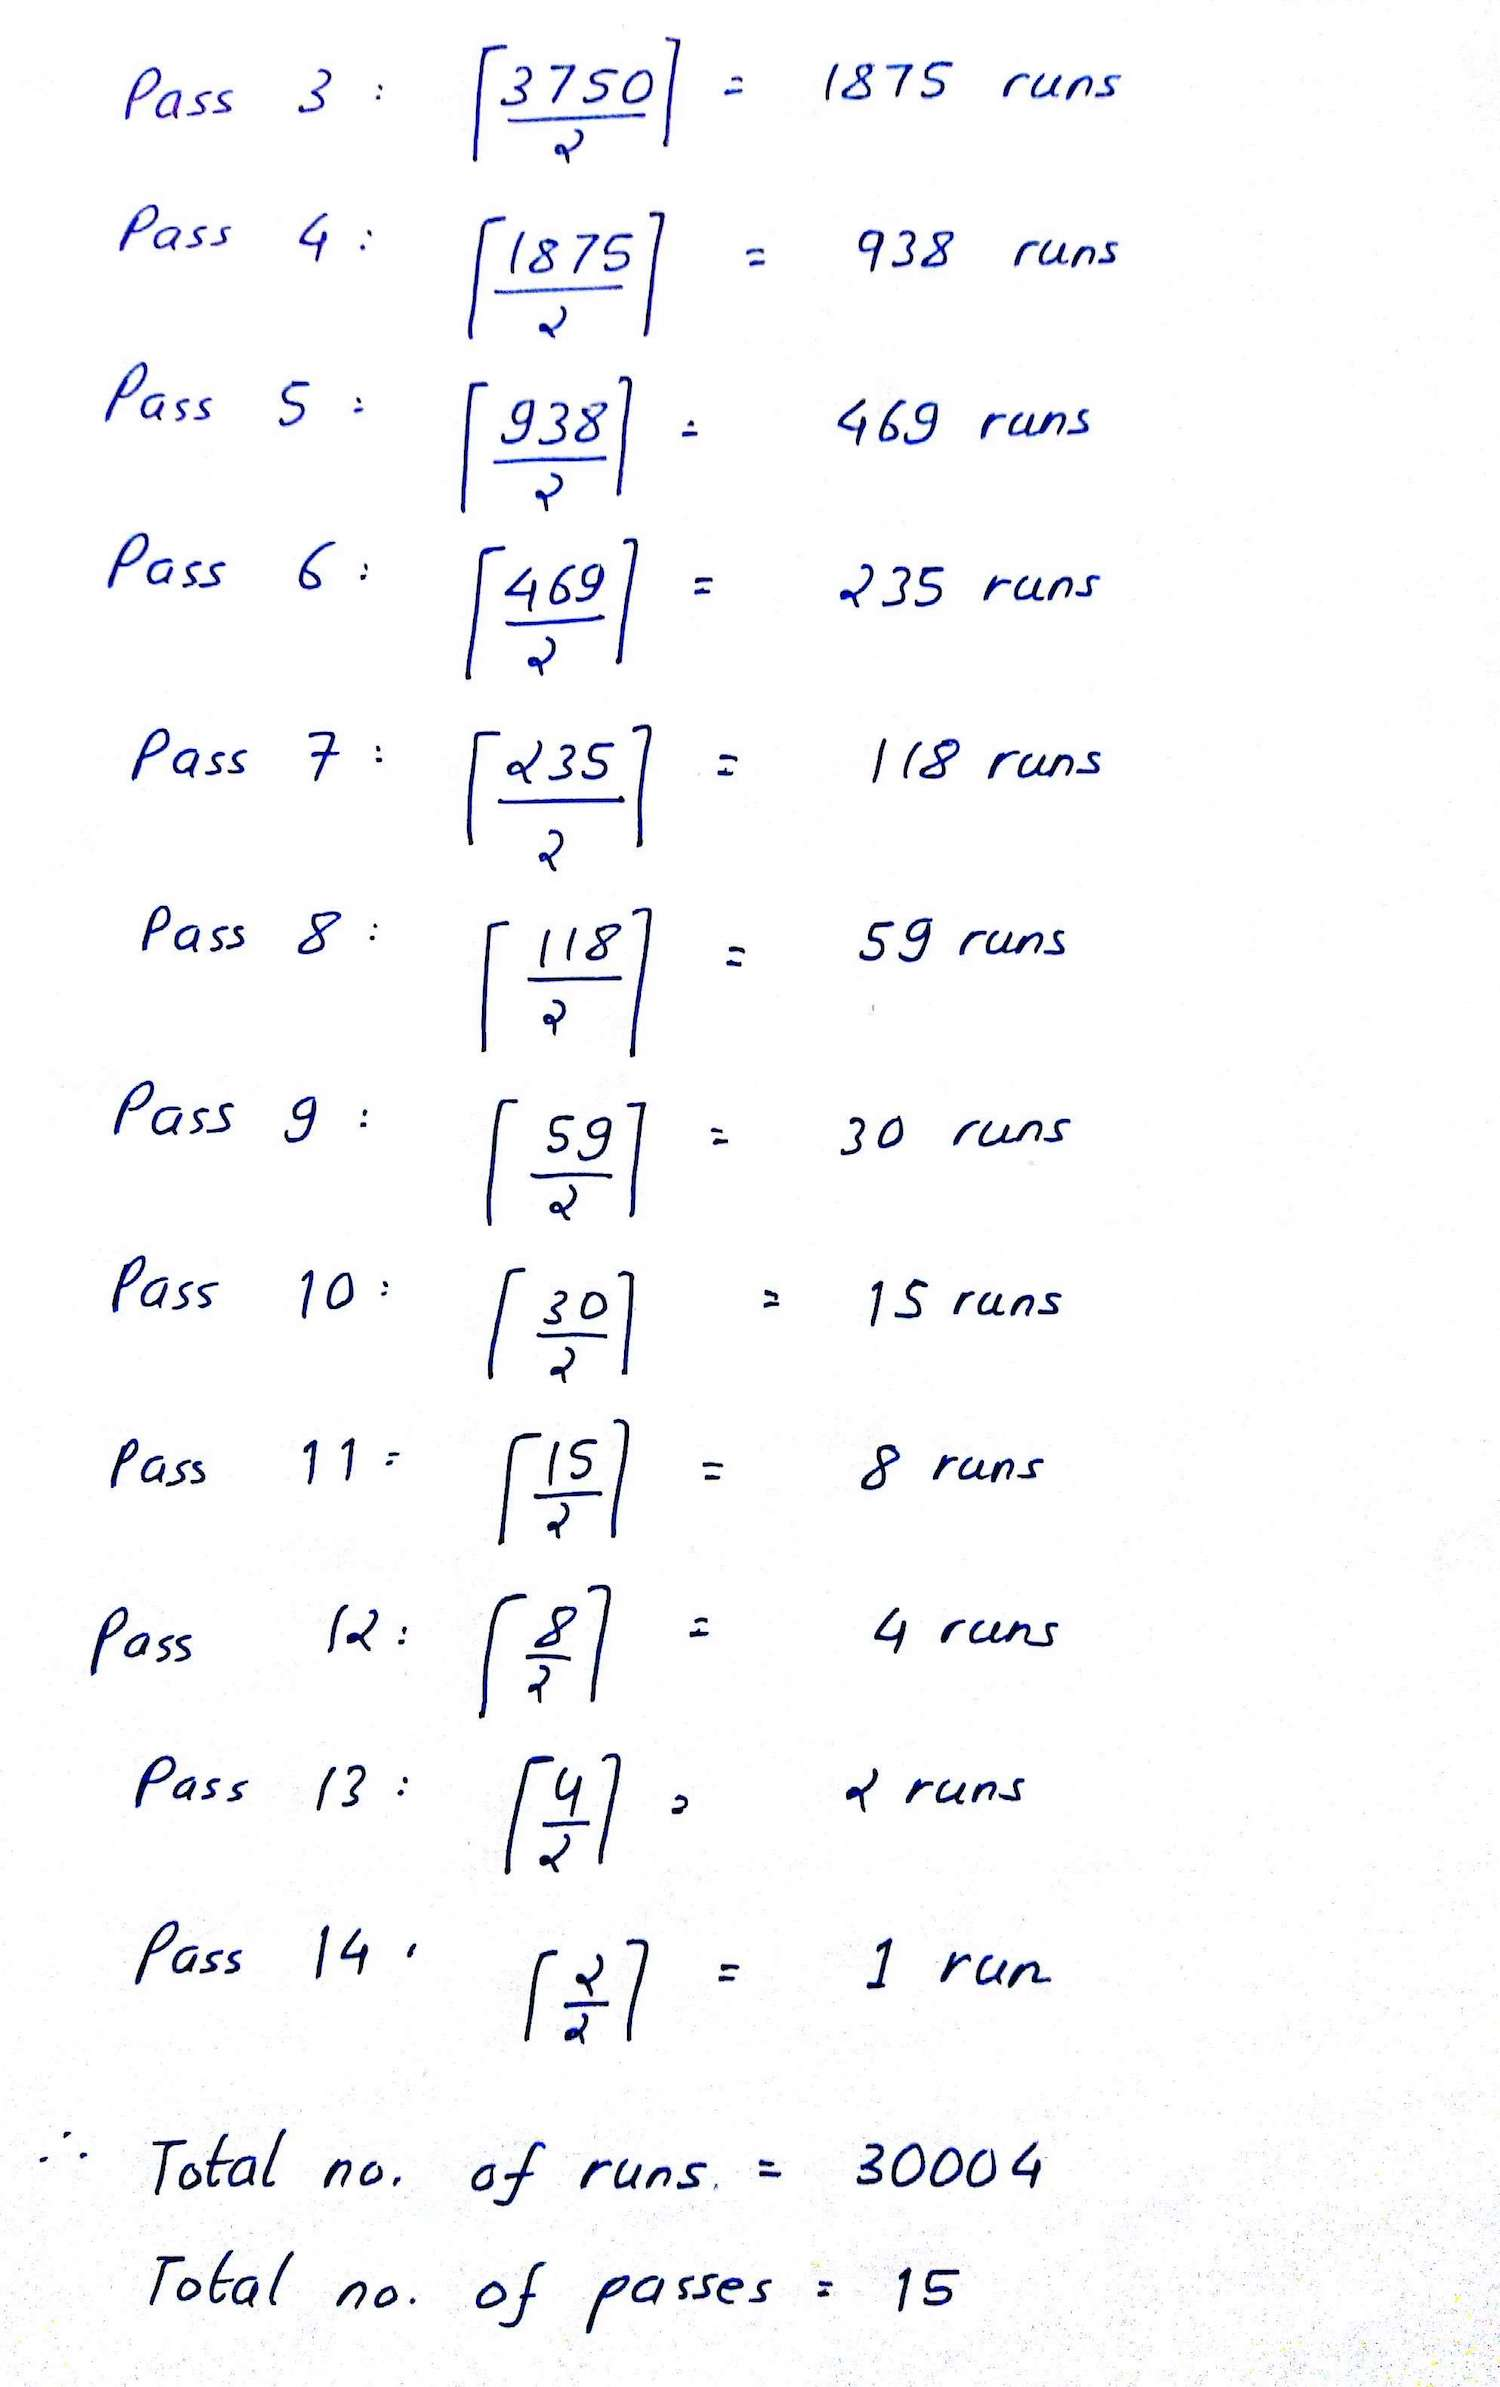
\includegraphics[width=12cm]{images/sol33.jpg}
\caption{Paper-based Solution for Question 3-3}
\end{figure} 

\end{homeworkProblem}

\begin{homeworkProblem}

\textbf{Part 1} \\
Calculate the I/O requirements of a simple nested loop join
 
 \vspace{0.1in} 
     \solution \\ \\ 
     %SOLUTION 
     In the expression below, M and N are the number of pages in the relations Album and Track respectively, $p_M$ and $p_N$ are the number of tuples in each page of the relations. \\
     
     \textbf{M as outer and N as inner relation} \\
     \textbf{Tuple-by-Tuple Simple Nested Loop Join} \\
     $M +  p_M \times M \times N$ \\
     $= 10000 + 100 \times 10000 \times 200000$ \\
     $ = 200000010000 $
          
    \vspace{0.1in}
     \textbf{Page-by-Page Simple Nested Loop Join} \\
     $M + M \times N$ \\
     $= 10000 + 10000 \times 200000$ \\
     $ = 2000010000 $
     
      \vspace{0.1in}
     \textbf{N as outer and M as inner relation} \\
     \textbf{Tuple-by-Tuple Simple Nested Loop Join} \\
     $N +  p_N \times N \times M$ \\
     $= 200000 + 80 \times 200000 \times 10000$ \\
     $ = 160000200000 $
          
    \vspace{0.1in}
     \textbf{Page-by-Page Simple Nested Loop Join} \\
     $M + M \times N$ \\
     $= 200000 + 200000 \times 10000$ \\
     $ = 2000200000 $
     \vspace{0.1in}
     
 \textbf{Part 2} \\
Calculate the I/O requirements of a block nested loop join
 
\vspace{0.1in} 
     \solution \\ \\ 
     %SOLUTION
     Block nested join for 16 buffers: \\
     
      \textbf{M as outer and N as inner relation} \\
     $ 10000 + \lceil \frac{10000}{14} \rceil \times 200000$
     $ = 143010000 $   
     \vspace{0.1in}
     
      \textbf{N as outer and M as inner relation} \\
      $ 200000 + \lceil \frac{200000}{14} \rceil \times 10000$
     $ = 143060000 $   
     \vspace{0.1in}
     
 \textbf{Part 3} \\
Explain the differences between the two algorithms. What are the similarities and differences? How does the block nested loop join reduce I/O costs?
 
 \vspace{0.1in} 
     \solution \\ \\ 
     %SOLUTION
     Tuple-at-a-time Simple Nested Loop Join scans outer relation and then for each tuple, it scans the entire inner relation. On the other hand, the page-at-a-time Simple Nested Loop Join will load the outer relation page-by-page, and then the inner relation for each page. The Block Nested Loop Join, on the other hand, scans entire inner relation for each block of pages in the outer relation. Therefore, the I/O cost of Block Nested Loop Join is lower than cost of both the Simple Nested Loop Joins. 
Moreover, the other important difference is number of buffer pages used in the algorithms. Both tuple-at-a-time nested loop and page-at-time nested loop join use 3 buffer pages to perform the join operation. 1 page as input buffer to scan outer relation,1 page as input buffer to scan inner relation  and 1 page as output buffer. Totally, 3 pages are needed for simple nested loop join. However, block nested loop join uses 1 page as input buffer to scan inner relation S and 1 page as output buffer. The other remaining buffer pages are used to load the blocks of the outer relation R. In this case, 1 buffer page is used as input buffer to scan inner relation  and 1 page as output buffer. Remaining 14 buffer pages are used to block outer relation . As seen, block nested loop join uses entire available buffer pages in the algorithm that means more efficient usage of buffer pages and causing performance increases and decreasing I/O cost. 

The similarities can be indicated as outer-inner relation usage, buffer usage and loop operations in the algorithms. 

     \vspace{0.1in}
     
\end{homeworkProblem}
     
\begin{homeworkProblem}
Given is a relation with 50.000 records. Each page for a node in a B+ tree can hold 20 pointers
to records or pages. A data page can store 20 records. \\

 \textbf{Part 1} \\
Assume that each node is 70 \% full. What is the height of the B+-tree? 

 \vspace{0.1in} 
     \solution \\ \\ 
     %SOLUTION  
     Given that the B+Tree can hold 20 pointers to pages. However, the B+ Tree has 70\% occupancy. Therefore, number of effective pointers to pages that the tree can hold,
     \begin{center} $ \implies 0.7 \times 20 = 14$ \end{center} 
Our B+ Tree can now be represented as Table 1

\begin{table}[]
\centering
\begin{tabular}{|l|l|l|l|}
\hline
Level    & Node & Entries & No. of Pointers \\ \hline
0 (Root) & 1    & 13      & 14              \\ \hline
1        & 14   & 182     & 196             \\ \hline
2        & 196  & 2548    & 2744         \\ \hline  
\end{tabular}
\caption{Different Levels of the B+ Tree}
\label{B+ Tree}
\end{table}

We have 2744 addresses in Level 2 already, which is more than 2500 pointers to pages required in the relations. \\
Therefore, the B-Tree has a depth of \textbf{3}.
Our B+ Tree has a depth of \textbf{3}
 \vspace{0.1in}
     
 \textbf{Part 2} \\
What are the I/O costs for an equality selection on a non-key attribute for the following
cases?

\begin{enumerate}[label = (\alph*)]
\item with a clustered B+-tree of height 3 (matching records are located in one page);
 
 \vspace{0.1in} 
     \solution \\ \\ 
     %SOLUTION
     The clustered index will guide the search, and after the end of the B+ tree traversal, we will need to input the correct page which contains our desired result. Therefore, total I/O is for the tree traversal and retrieving the correct page, i.e. 3 I/Os + 1 I/O = 4.
     Hence, total number of I/Os = \textbf{4} I/Os
     \vspace{0.1in}
     
\item without any index, nor is the file sorted on the attribute occurring in selection;

\vspace{0.1in} 
     \solution \\ \\ 
     %SOLUTION 
     Total number of pages at the leaf node = 2500
    If we consider that all pages need to be scanned, then the I/O costs will be \textbf{2500} I/Os. \\
    However, assuming, on an average that half the total number of pages need to be searched to find the equality results, it gives a total of 1250 I/Os.
          
     \vspace{0.1in}
     
\item with an unclustered B+-tree index of height 4, and there are 2 matching records;

\vspace{0.1in} 
     \solution \\ \\ 
     4 I/Os to traverse the tree + 2 I/Os to retrieve the matching records = \textbf{6} I/Os 
     \vspace{0.1in}

\item with an unclustered B+-tree of height 5 and three tenth of the records match the
selection.

\vspace{0.1in} 
\solution \\ \\ 
     %SOLUTION
     No. of matching records = $\frac{3}{10} \times 50000 = 15000$ records \\
     In the worst case, we need to do 15000 page I/Os, one for each record. Plus the I/Os for traversing the tree. Therefore, a total of 15000 I/Os + 5 I/Os = \textbf{15005} I/Os.   
     \vspace{0.1in}

\end{enumerate}
\end{homeworkProblem}

\end{document}
\documentclass[12pt]{article}

\usepackage{fancyhdr}
\usepackage{extramarks}
\usepackage{amsmath}
\usepackage{amsthm}
\usepackage{amsfonts}
\usepackage{tikz}
\usepackage[plain]{algorithm}
\usepackage{algpseudocode}
\usepackage[export]{adjustbox}
\usepackage[latin1]{inputenc}           %For German characters
\usepackage{enumitem}               %For changing enumeration character
\usepackage{listings}               %For code
\usepackage{csquotes}
\usepackage{graphicx}               %For graphics e.g, images

\usetikzlibrary{automata,positioning}

%
% Basic Document Settings
%

\topmargin=-0.45in
\evensidemargin=0in
\oddsidemargin=0in
\textwidth=6.5in
\textheight=9.0in
\headsep=0.25in

\linespread{1.1}

\pagestyle{fancy}
\lhead{\hmwkAuthorName}
\chead{\hmwkClass\ : \hmwkTitle}
\rhead{\firstxmark}
\lfoot{\lastxmark}
\cfoot{\thepage}

\renewcommand\headrulewidth{0.4pt}
\renewcommand\footrulewidth{0.4pt}

\setlength\parindent{0pt}

%
% Create Problem Sections
%

\newcommand{\enterProblemHeader}[1]{
    \nobreak\extramarks{}{Problem \arabic{#1} continued on next page\ldots}\nobreak{}
    \nobreak\extramarks{Problem \arabic{#1} (continued)}{Problem \arabic{#1} continued on next page\ldots}\nobreak{}
}

\newcommand{\exitProblemHeader}[1]{
    \nobreak\extramarks{Problem \arabic{#1} (continued)}{Problem \arabic{#1} continued on next page\ldots}\nobreak{}
    \stepcounter{#1}
    \nobreak\extramarks{Problem \arabic{#1}}{}\nobreak{}
}

\setcounter{secnumdepth}{0}
\newcounter{partCounter}
\newcounter{homeworkProblemCounter}
\setcounter{homeworkProblemCounter}{1}
\nobreak\extramarks{Problem \arabic{homeworkProblemCounter}}{}\nobreak{}

%
% Homework Problem Environment
%
% This environment takes an optional argument. When given, it will adjust the
% problem counter. This is useful for when the problems given for your
% assignment aren't sequential. See the last 3 problems of this template for an
% example.
%
\newenvironment{homeworkProblem}[1][-1]{
    \ifnum#1>0
        \setcounter{homeworkProblemCounter}{#1}
    \fi
    \section{Problem \arabic{homeworkProblemCounter}}
    \setcounter{partCounter}{1}
    \enterProblemHeader{homeworkProblemCounter}
}{
    \exitProblemHeader{homeworkProblemCounter}
}

%
% Homework Details
%   - Title
%   - Due date
%   - Class
%   - Section/Time
%   - Instructor
%   - Author
%

\newcommand{\hmwkTitle}{Assignment\ \#2}
\newcommand{\hmwkDueDate}{November 15, 2016}
\newcommand{\hmwkClass}{Implementation of Databases}
\newcommand{\hmwkAuthorName}{Sanchit Alekh}
\newcommand{\hmwkClassTime}{MSc. Software Systems Engineering}
\newcommand{\hmwkClassInstructor}{Universitätsprofessor Dr. rer. pol. Matthias Jarke}
\newcommand{\hmwkClassInstructors}{Dr. rer. nat. Christoph Quix}

%
% Title Page
%



\title{
   \begin{center}
   \vspace*{-20mm}
   
\includegraphics[width=0.4\textwidth, right]{images/rwth_logo.png}
   \\
   \vspace*{3cm}
    \textmd{\textbf{\hmwkClass}}\\
    \textmd{\textbf{\hmwkTitle}}\\
    \normalsize\vspace{0.1in}\small{Due\ on\ \hmwkDueDate } \\
    \vspace{0.1in}\large{\textit{\hmwkClassInstructor}} \\
    \vspace{0.1in}\large{\textit{\hmwkClassInstructors}} \\
    \vspace{3in}
     \textbf{Submitted by:} \\
     \vspace{0.25in}
    \large{Sanchit Alekh, Idil Esen Zülfikar, Nihal Hegde} \\
    %\author{\textbf{\hmwkAuthorName}}
    \vspace{0.1in} \large{\textit{\hmwkClassTime}} \\
    %\vspace{0.1in} \large{\textit{Matrikelnummer : 359831}}
    \end{center}
    }


\date{}

\renewcommand{\part}[1]{\textbf{\large Part \Alph{partCounter}}\stepcounter{partCounter}\\}

%
% Various Helper Commands
%

% Useful for algorithms
\newcommand{\alg}[1]{\textsc{\bfseries \footnotesize #1}}

% For derivatives
\newcommand{\deriv}[1]{\frac{\mathrm{d}}{\mathrm{d}x} (#1)}

% For partial derivatives
\newcommand{\pderiv}[2]{\frac{\partial}{\partial #1} (#2)}

% Integral dx
\newcommand{\dx}{\mathrm{d}x}

% Alias for the Solution section header
\newcommand{\solution}{\textbf{\large Solution}}

% Probability commands: Expectation, Variance, Covariance, Bias
\newcommand{\E}{\mathrm{E}}
\newcommand{\Var}{\mathrm{Var}}
\newcommand{\Cov}{\mathrm{Cov}}
\newcommand{\Bias}{\mathrm{Bias}}

\begin{document}

\maketitle

\pagebreak

\begin{homeworkProblem}
    
    \textbf{Part 1} \\
    Variants of relational algebra are used internally in DBMS to represent queries and query evaluation plans. Please explain, why relational algebra is suitable for this?
    
    \vspace{0.1in}
    \solution \\
    One of the most desirable properties of Relational Algebra is that queries are composed using a collection of operators, and every operator accepts one or two relation instances as arguments and returns a relation instance as the result. This property makes extremely easy and efficient to compose operators to form a complex query. A relational algebra expression can be recursively defined to be a relation, a unary algebra operator applied to a single expression, or a binary algebra operator applied to two expressions. 
This procedural nature of relational algebra is the main reason why it is used internally in DBMS to represent queries and evaluation plans. The approach allows us to think of an algebra expression as an imperative execution plan for a declarative SQL query. It can be used for evaluating a query, and relational systems in fact use algebra expressions to represent query evaluation plans.
        
    \vspace{0.1in}
    
    \textbf{Part 2} \\
    What does \enquote{relational completeness} mean (in your own words, please)? Show that SQL is
relationally complete by enumerating SQL constructs corresponding to selection, projection,
cartesian product, union, and difference.
    
    \vspace{0.1in}
    \solution \\
    \enquote{Relational Completeness} of a query methodology means that each and every query that can be expressed using that methodology, can also be expressed as a relational algebra query. In this case, SQL is referred to as \enquote*{Relationally Complete} because every legal construct in SQL can be expressed as a Relational Algebra query.
        
These are the examples of Relational Algebra expressions and their equivalent expressions in SQL. The following examples are derived from the \textit{Mondial} database.

\begin{itemize}

\item \textbf{SELECTION} \\
Relational Algebra: $ \sigma_{Area > 650} (Island)$ \\
SQL:  \textit{Select * From Island Where Area $>$ 650;}

\item \textbf{PROJECTION} \\
Relational Algebra: $ \pi_{Name, Islands, Area, Height} (Island)$ \\
SQL: \textit{Select Name, Islands, Area, Height From Island;}

\item \textbf{CARTESIAN PRODUCT} \\
Relational Algebra:  $ Island \times islandIn$ \\
SQL: \textit{Select * From Island CROSS JOIN islandIn;}

\item \textbf{UNION} \\
Relational Algebra:  $ \pi_{name} (Desert) \cup \pi_{name} (geo\_Desert)$ \\
SQL: \textit{Select name From Desert or Select name From geo\_Desert}

\item \textbf{SET DIFFERENCE} \\
Relational Algebra: $ \pi_{name} (\sigma_{height > 5000} (Mountain)) - \pi_{name}( \sigma_{type > 'volcanic')} (Mountain) $ \\
SQL: \textit{Select name From Mountain where height $>$ 5000 MINUS Select name From Mountain where type='volcanic'}
\end{itemize}
        
    \vspace{0.1in}
        
     \textbf{Part 3} \\
    Explain how the intersection operator is used in relational algebra. What is important for
its usage? Is it omittable (i.e., could you express it by other operators)? If so, please give
the corresponding relational algebra.
    
    \vspace{0.1in}
    \solution \\
    The \enquote*{Intersection} operator is represented in Relational Algebra with the help of the $\cap$ symbol. Although it is not a fundamental set-operator, it is an extremely widely used operation, and it is helpful to define it separately. An example use of the intersection operator is as follows:
    
    \begin{center} $ \pi_{name} (Desert) \cap \pi_{name} (geo\_Desert) $ \end{center}
    
The important condition for using the \textit{Intersection} operator is that the two sets which have to be intersected must be \textit{union-compatible}. This follows from the fact that intersection is defined in terms of set difference.

Yes, Intersection is not a fundamental set-operator, and it can be expressed in terms of the set-difference operator. Therefore, it is omittable. A general expression for the intersection operator in terms of the set-difference operator is:

    \begin{center} $ A \cup B \leftrightarrow A \setminus ( A \setminus B) $ \end{center}
    
Therefore, the example Relational Algebra query illustrated above can be represented by the equivalent query without the use of set-intersection as follows:

    \begin{center} $ \pi_{name} (Desert) - (\pi_{name} (Desert) - \pi_{name} (geo\_Desert))$ \end{center}
    
\begin{figure}[h]
\centering
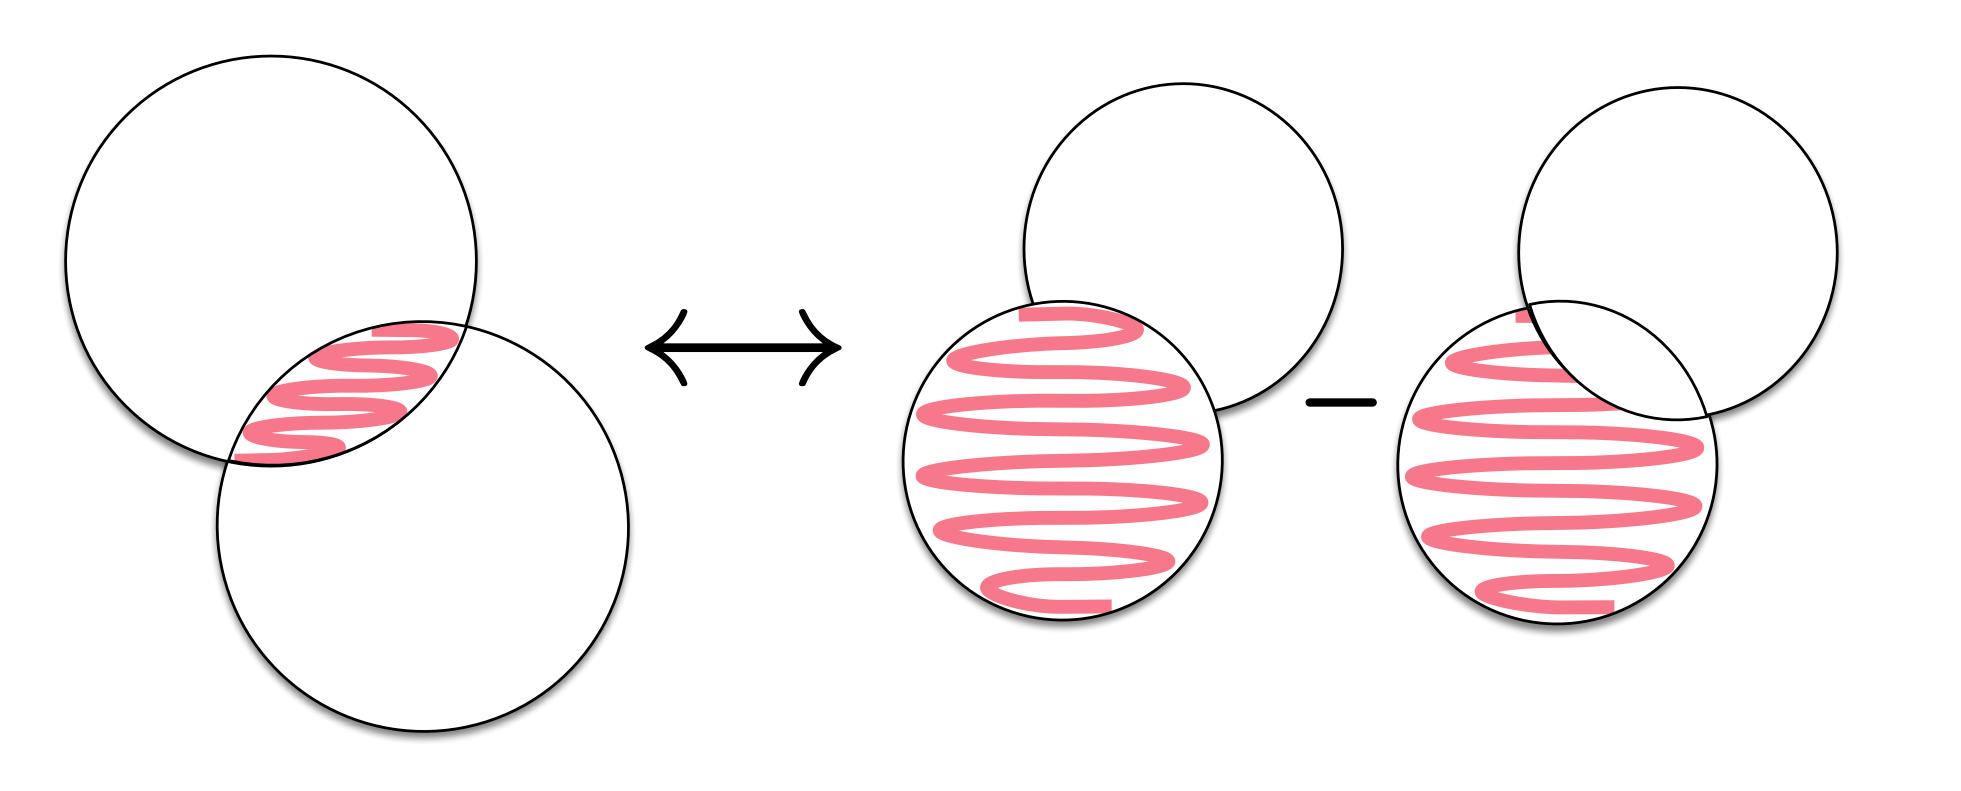
\includegraphics[width=12cm]{images/intersection1.png}
\caption{Venn-Diagram showing the definition of Intersection in terms of Set Difference}
\end{figure}
        
    \vspace{0.1in}
    
     \textbf{Part 4} \\
    Explain the difference between DRC and TRC.
    
    \vspace{0.1in}
        \solution \\
In Tuple Relational Calculus (TRC), the variables typically range over tuples, i.e. they directly represent tuples. On the other hand, in Domain Relational Calculus (DRC), the variables range over domain elements, i.e. field values. In TRC, tuples are semantically equivalent to variables, i.e. field referencing can be used to select tuple parts. On the other hand, in DRC, formal variables are explicit and have to be defined.
    \vspace{0.1in}
    
    
\end{homeworkProblem}   

\begin{homeworkProblem}

\textbf{Part 1} \\

The names of the seas that are deeper than 3000 mt and into which at least one river finally flows.

\vspace{0.1in}
    \solution \\
      
    $<name> \mid \exists depth, rname, river, lake, sea, length, sLong, sLat, mount, sAlt, estLong, estLat \\
    Sea(name, depth) \wedge  \\ River(rname, river, lake, sea, length, sLong, sLat, mount, sAlt, estLong, estLat) \wedge \\ depth > 3000 \wedge sea = name$ 
    \vspace{0.1in}
    
\textbf{Part 2} \\
The names of the groups of islands that consist only of islands that are neither 'volcanic' nor
'coral'.

 \vspace{0.1in}
    \solution \\ \\    
   %SOLUTION
   $<islands> \mid \exists name, area, height, type, long, lat \\
Island(name, islands, area, height, type, long, lat) \wedge \\
type \notin \{volcanic, coral\} \wedge islands \neq \emptyset  $
    \vspace{0.1in}    

\textbf{Part 3} \\
The name of the mountain, the name of the mountains where it belongs to and the name of
the country where the mountain is located for each mountain that is located on an island
that is of type 'coral'.

 
 \vspace{0.1in} 
     \solution \\ \\ 
     %SOLUTION   
     $<moiMountain, mMountains, gmCountry> \mid \exists \\ moiIsland, mHeight, mType, mLong, mLat, \\ iIslands, iArea, iHeight, iType, iLong, iLat, gmProvince \\
mountainOnIsland(moiMountain, moiIsland) \wedge \\ Mountain(moiMountain, mMountains, mHeight, mType, mLong, mLat) \wedge \\ geo\_Mountain(moiMountain, gmCountry, gmProvince)  \wedge \\
Island(moiIsland, iIslands, iArea, iHeight, iType, iLong, iLat) \wedge iType \neq "coral" $

     \vspace{0.1in}

    
\textbf{Part 4} \\
Give the name and country name of all cities with a population higher than 500,000.

 \vspace{0.1in} 
     \solution \\ \\    
    %SOLUTION
   $<cName, coName> \mid \exists cCountry, cProvince, cPopulation, cLong, cLat, \\
   coCapital, coProvince, coArea, coPopulation \\
City(cName, cCountry, cProvince, cPopulation, cLong, cLat)  \wedge \\
Country(cCountry, coName, coCapital, coProvince, coArea, coPopulation) \wedge \\
cPopulation > 500000 $
 
    \vspace{0.1in}
        
\end{homeworkProblem}

\begin{homeworkProblem}
Suppose you have a file of 15,000 pages and eight buffer pages and you are sorting it using general
(external) merge-sort. Please answer the following questions: \\

\textbf{Part 1} \\
How many runs will you produce? Remark: When a file is sorted, in intermediate steps
subfiles are created. Each sorted subfile is called a run. See also slide 35 in Chapter 2.
 \textbf{Note: Detailed solution of Q3 is produced in \textit{Figures 2, 3 and 4.}}
 
 \vspace{0.1in} 
     \solution \\
     %SOLUTION
     \textbf{2189} runs will be produced   
     \vspace{0.1in}
     
 \textbf{Part 2} \\
How many passes will it take to sort the file completely?
 
 \vspace{0.1in} 
     \solution \\ 
    It will take \textbf{5} passes   
     \vspace{0.1in}
     
 \textbf{Part 3} \\
How many buffer pages do you need at least to sort the file in two passes? 

 \vspace{0.1in} 
     \solution \\
     With \textbf{123} buffers, you can sort the file in two passes 
     \vspace{0.1in}
 
 \textbf{Part 4} \\
How many runs and passes would a Two-Way-Sort algorithm take?
 
 \vspace{0.1in} 
     \solution \\
     %SOLUTION
     Two-Way Sort Algorithm will take \textbf{30004} runs and \textbf{15} passes   
     \vspace{0.1in}   
     
\begin{figure}[h]
\centering
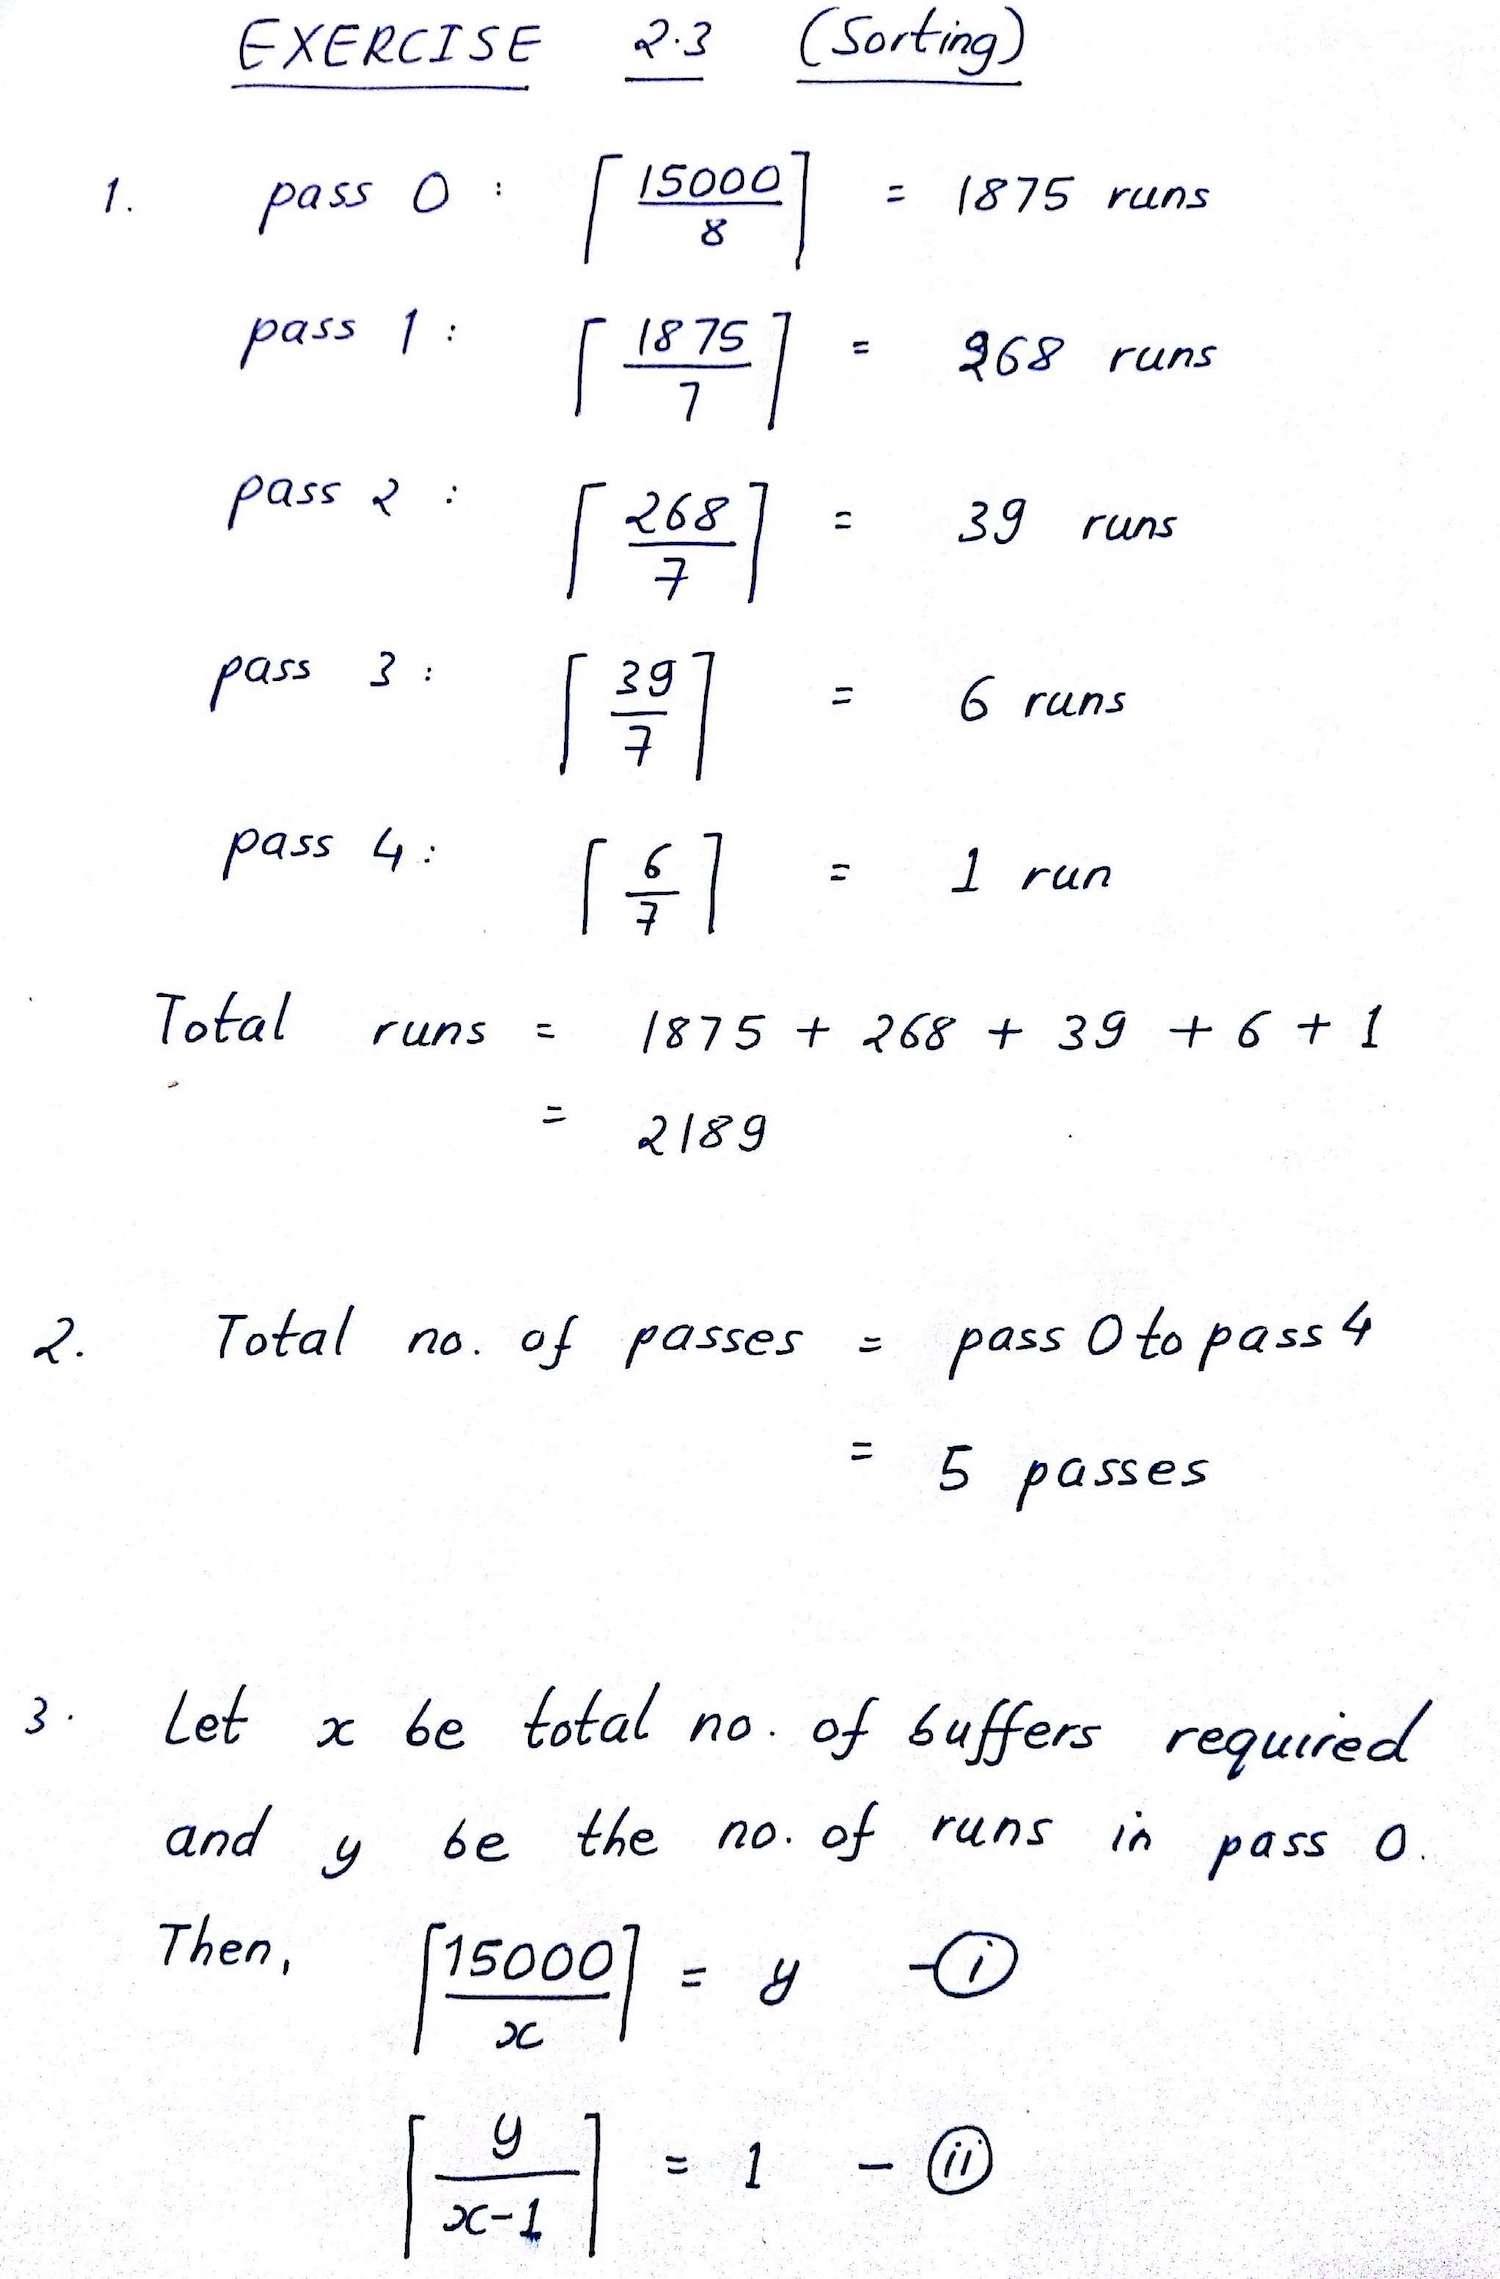
\includegraphics[width=12cm]{images/sol31.jpg}
\caption{Paper-based Solution for Question 3-1}
\end{figure} 

\begin{figure}[h]
\centering
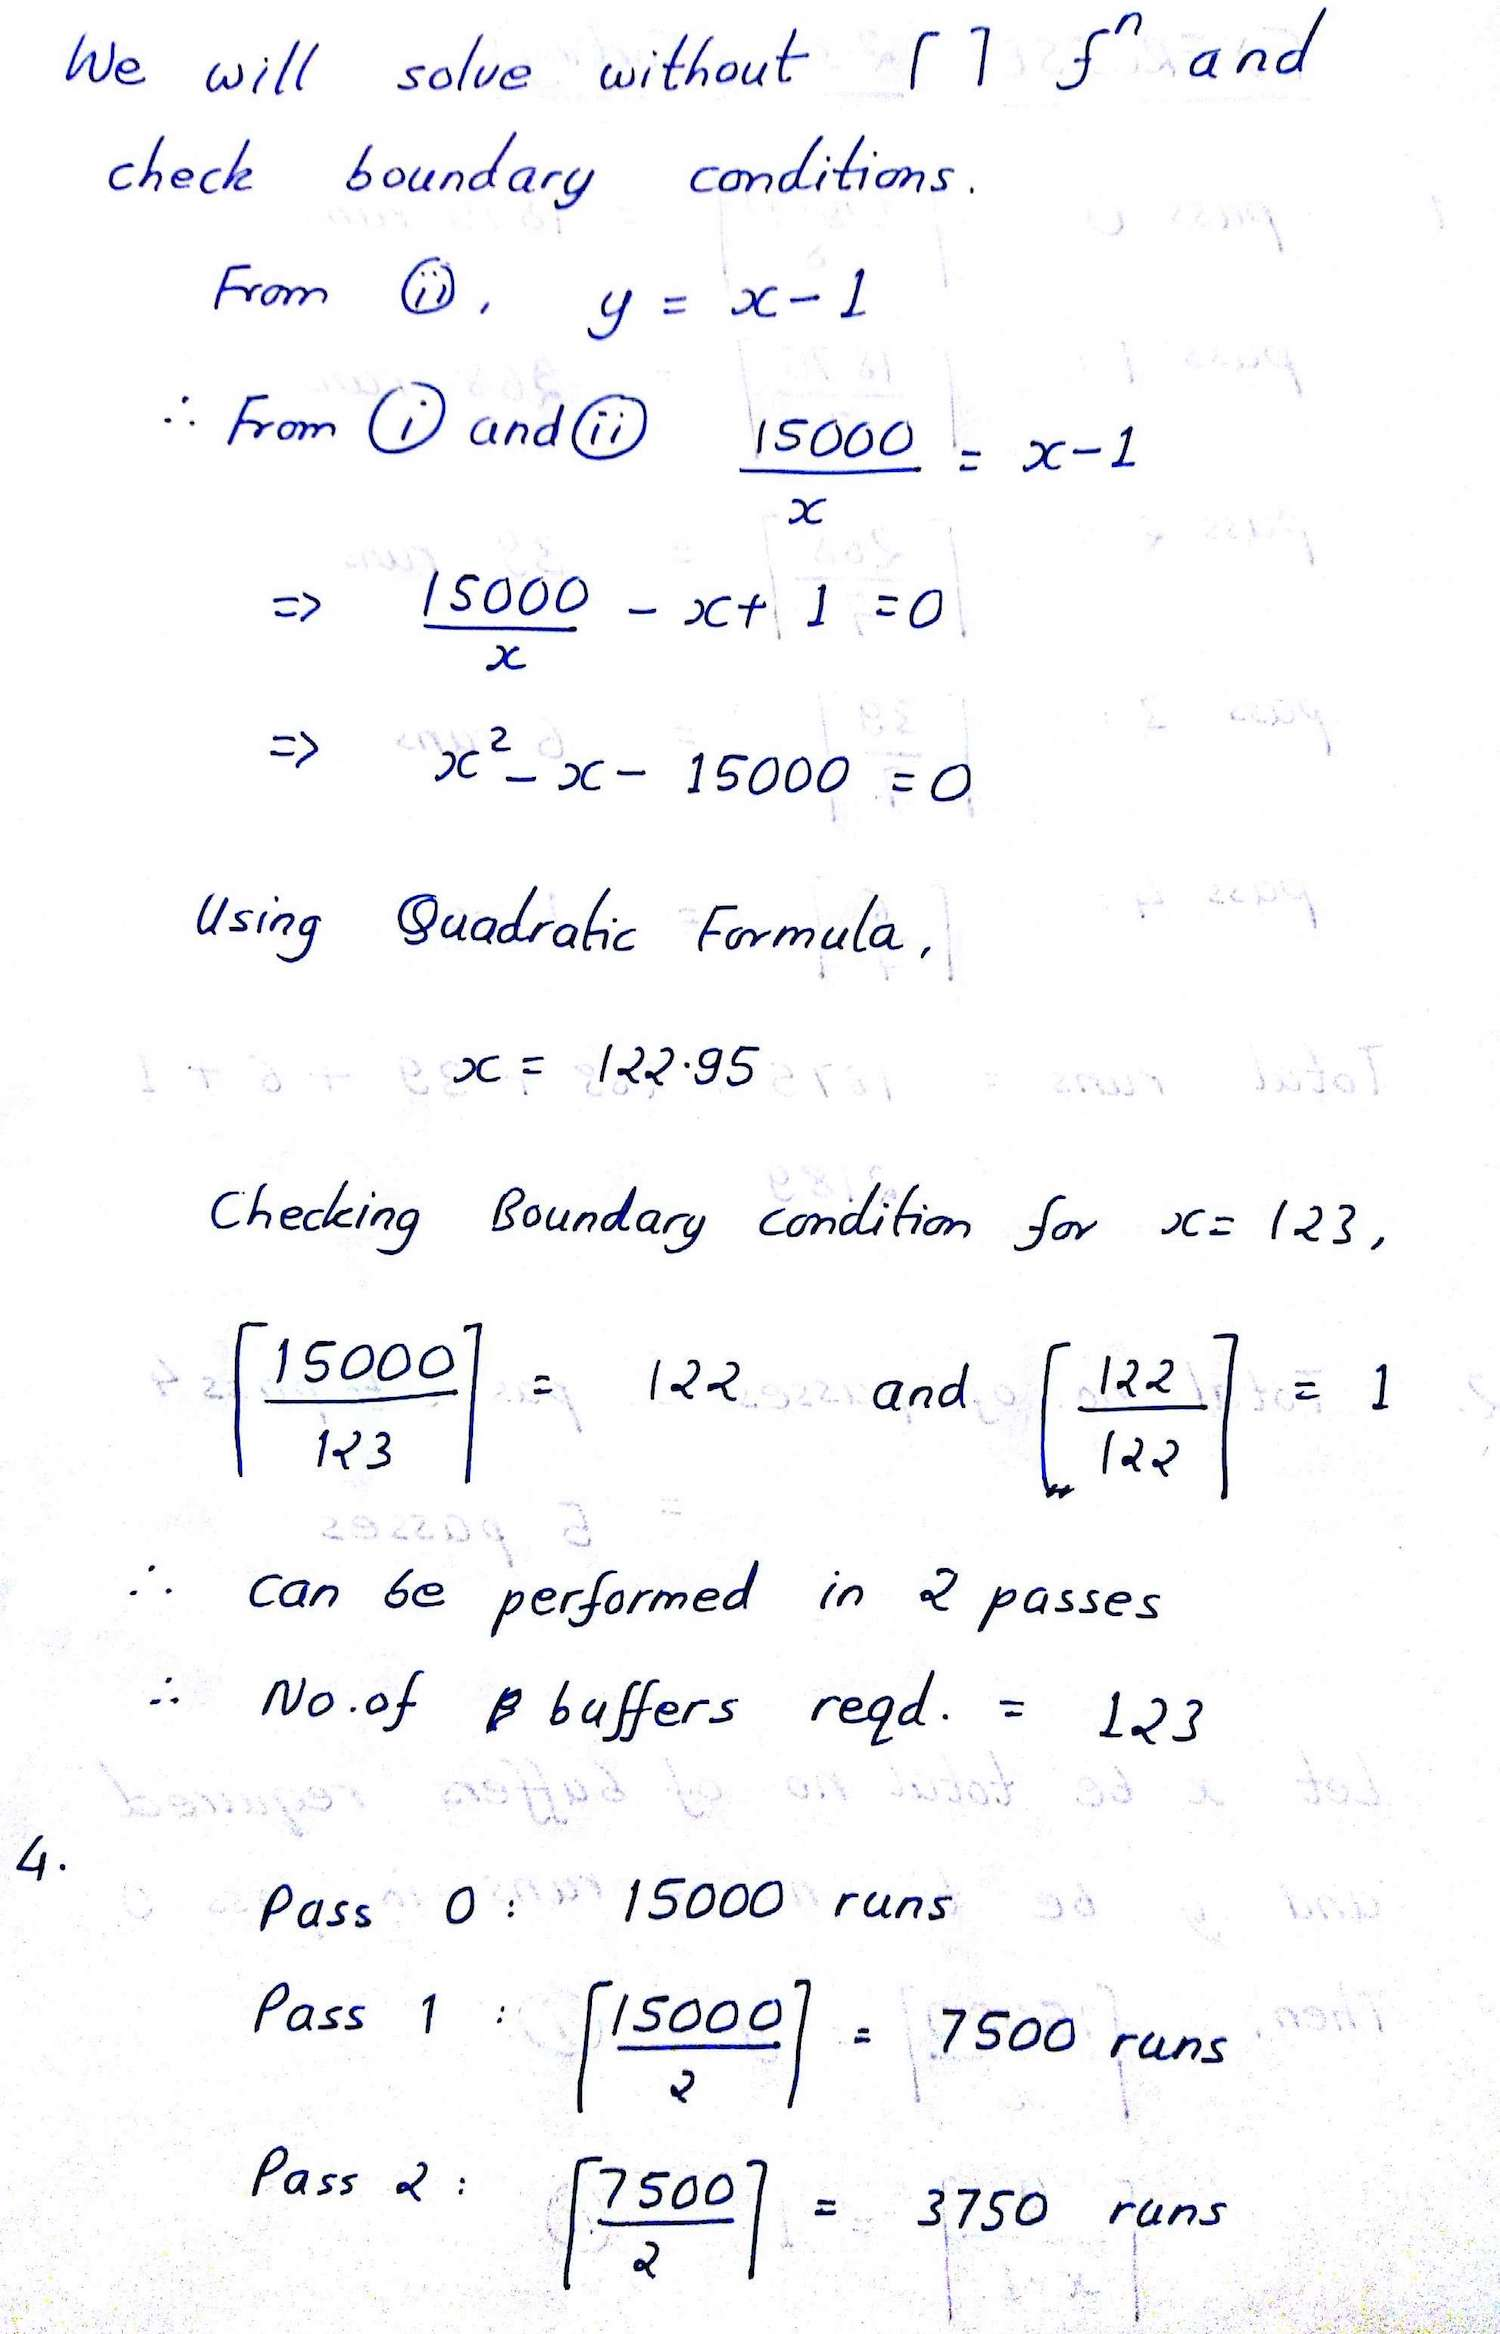
\includegraphics[width=12cm]{images/sol32.jpg}
\caption{Paper-based Solution for Question 3-2}
\end{figure} 

\begin{figure}[h]
\centering
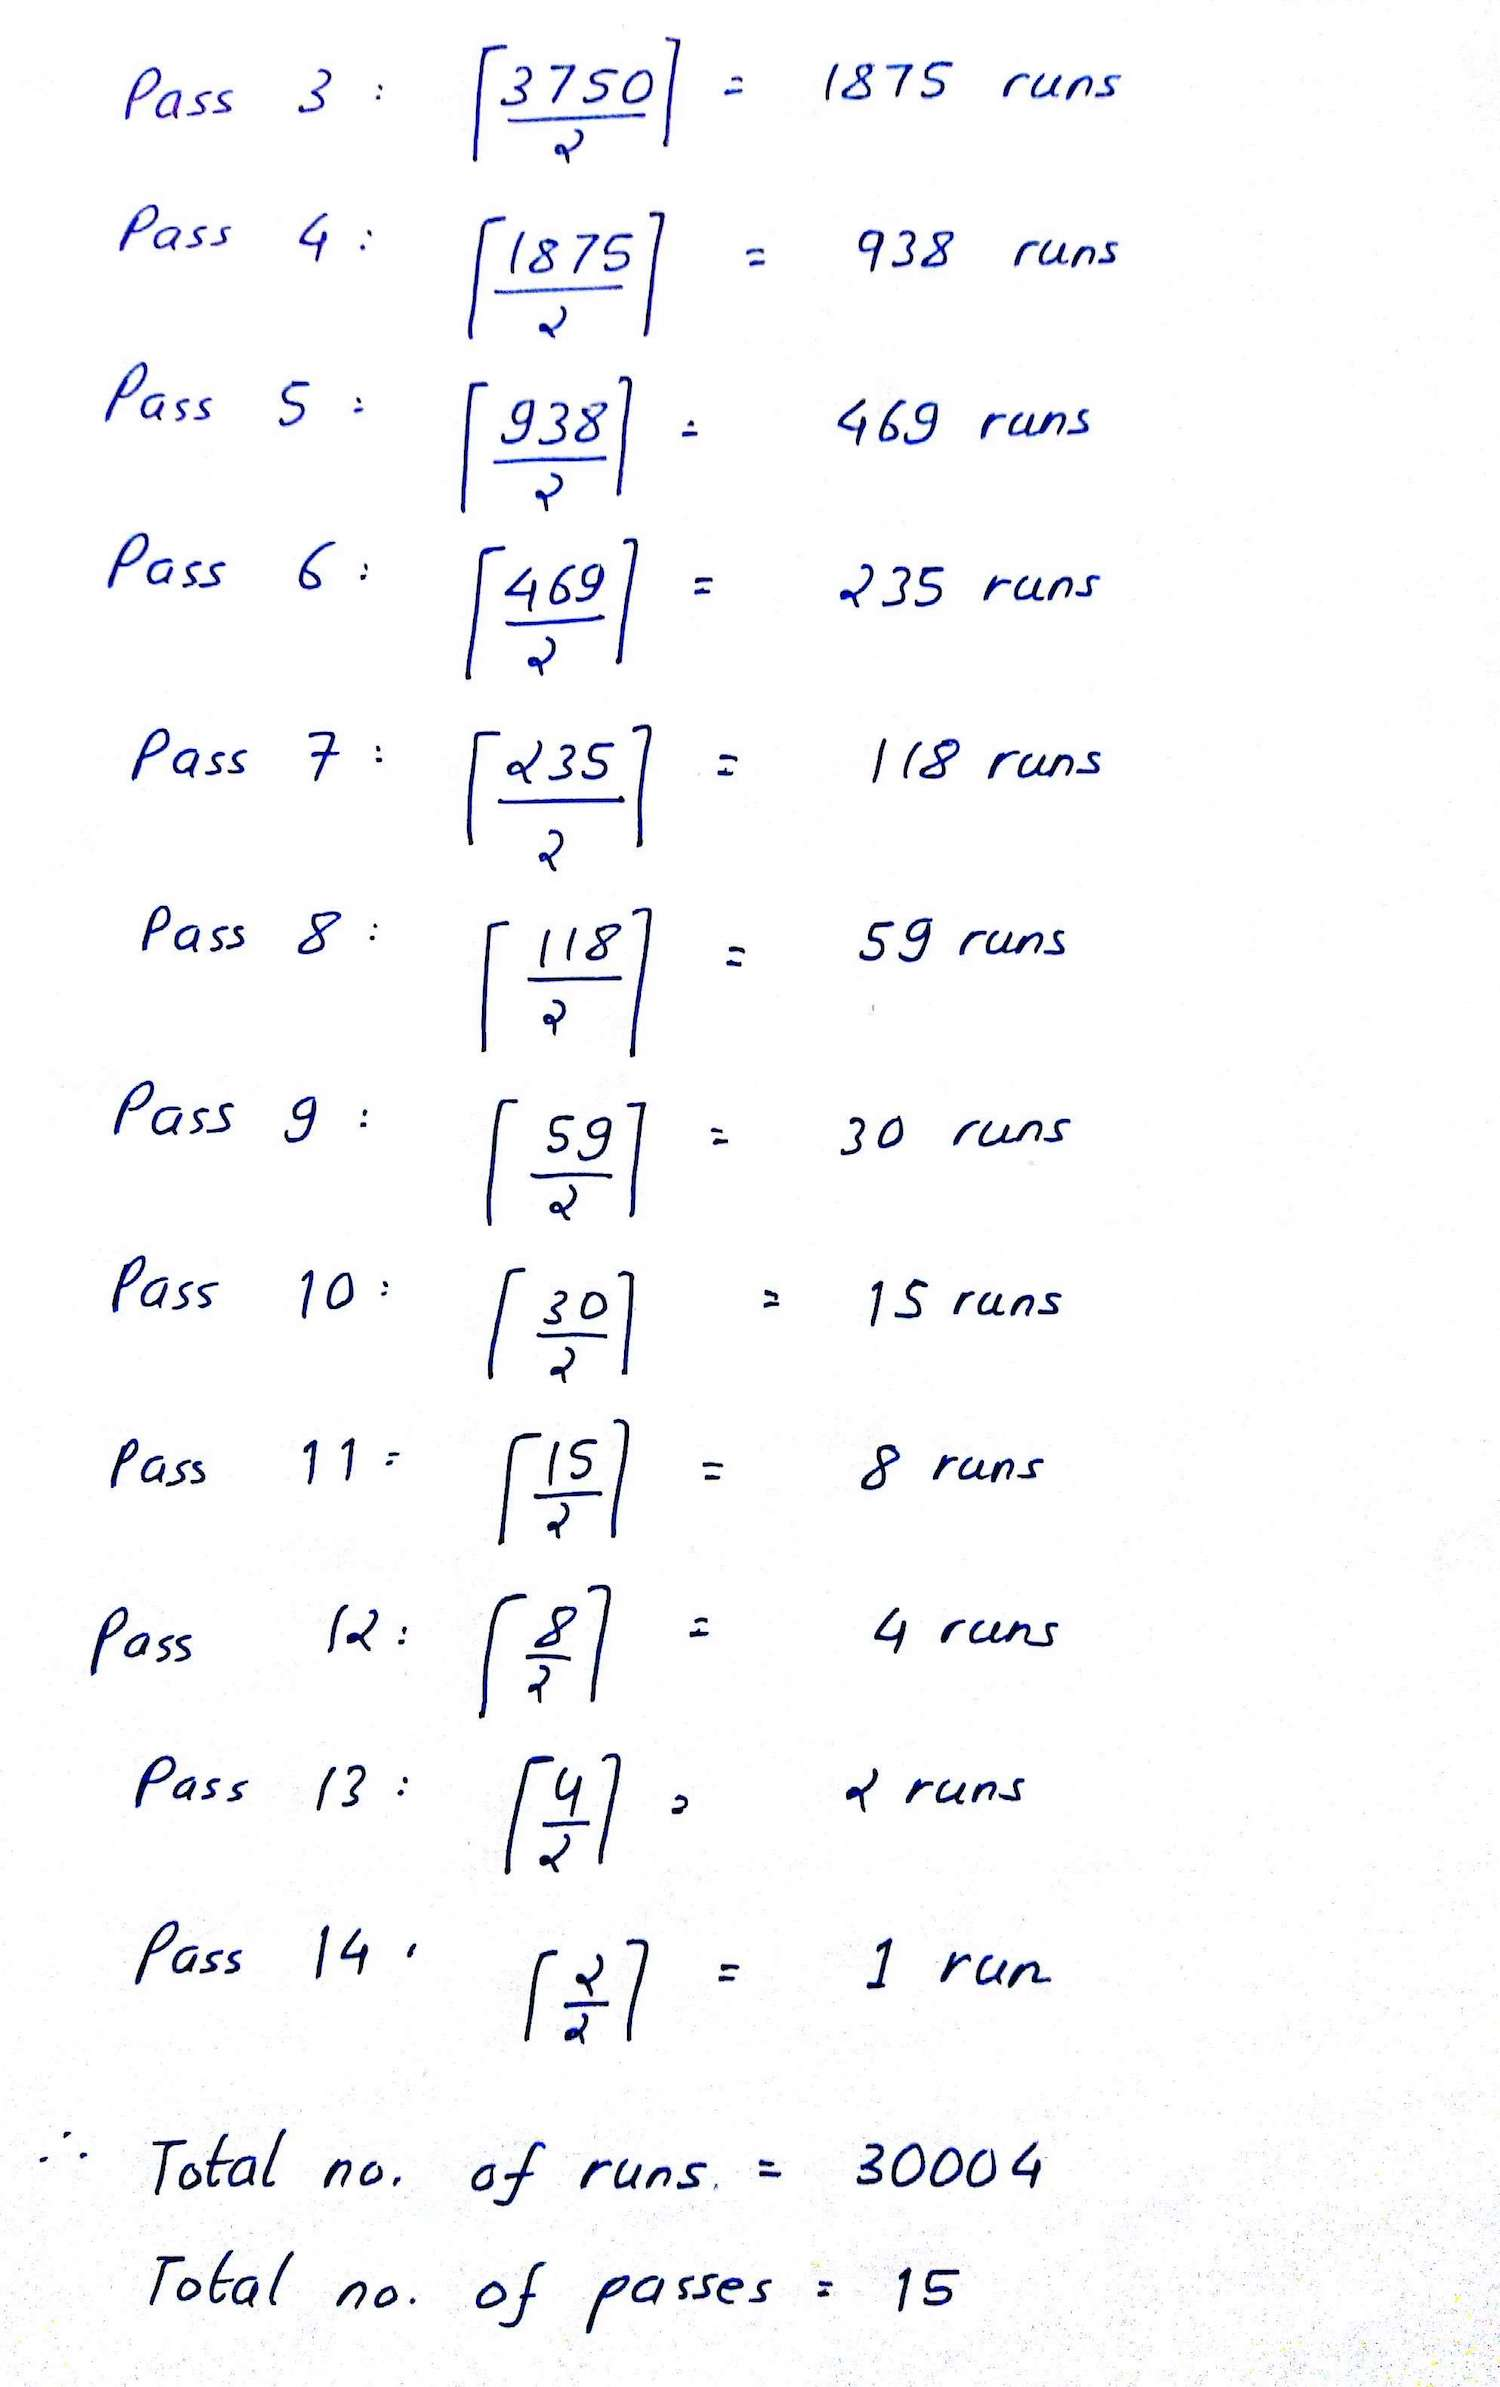
\includegraphics[width=12cm]{images/sol33.jpg}
\caption{Paper-based Solution for Question 3-3}
\end{figure} 

\end{homeworkProblem}

\begin{homeworkProblem}

\textbf{Part 1} \\
Calculate the I/O requirements of a simple nested loop join
 
 \vspace{0.1in} 
     \solution \\ \\ 
     %SOLUTION 
     In the expression below, M and N are the number of pages in the relations Album and Track respectively, $p_M$ and $p_N$ are the number of tuples in each page of the relations. \\
     
     \textbf{M as outer and N as inner relation} \\
     \textbf{Tuple-by-Tuple Simple Nested Loop Join} \\
     $M +  p_M \times M \times N$ \\
     $= 10000 + 100 \times 10000 \times 200000$ \\
     $ = 200000010000 $
          
    \vspace{0.1in}
     \textbf{Page-by-Page Simple Nested Loop Join} \\
     $M + M \times N$ \\
     $= 10000 + 10000 \times 200000$ \\
     $ = 2000010000 $
     
      \vspace{0.1in}
     \textbf{N as outer and M as inner relation} \\
     \textbf{Tuple-by-Tuple Simple Nested Loop Join} \\
     $N +  p_N \times N \times M$ \\
     $= 200000 + 80 \times 200000 \times 10000$ \\
     $ = 160000200000 $
          
    \vspace{0.1in}
     \textbf{Page-by-Page Simple Nested Loop Join} \\
     $M + M \times N$ \\
     $= 200000 + 200000 \times 10000$ \\
     $ = 2000200000 $
     \vspace{0.1in}
     
 \textbf{Part 2} \\
Calculate the I/O requirements of a block nested loop join
 
\vspace{0.1in} 
     \solution \\ \\ 
     %SOLUTION
     Block nested join for 16 buffers: \\
     
      \textbf{M as outer and N as inner relation} \\
     $ 10000 + \lceil \frac{10000}{14} \rceil \times 200000$
     $ = 143010000 $   
     \vspace{0.1in}
     
      \textbf{N as outer and M as inner relation} \\
      $ 200000 + \lceil \frac{200000}{14} \rceil \times 10000$
     $ = 143060000 $   
     \vspace{0.1in}
     
 \textbf{Part 3} \\
Explain the differences between the two algorithms. What are the similarities and differences? How does the block nested loop join reduce I/O costs?
 
 \vspace{0.1in} 
     \solution \\ \\ 
     %SOLUTION
     Tuple-at-a-time Simple Nested Loop Join scans outer relation and then for each tuple, it scans the entire inner relation. On the other hand, the page-at-a-time Simple Nested Loop Join will load the outer relation page-by-page, and then the inner relation for each page. The Block Nested Loop Join, on the other hand, scans entire inner relation for each block of pages in the outer relation. Therefore, the I/O cost of Block Nested Loop Join is lower than cost of both the Simple Nested Loop Joins. 
Moreover, the other important difference is number of buffer pages used in the algorithms. Both tuple-at-a-time nested loop and page-at-time nested loop join use 3 buffer pages to perform the join operation. 1 page as input buffer to scan outer relation,1 page as input buffer to scan inner relation  and 1 page as output buffer. Totally, 3 pages are needed for simple nested loop join. However, block nested loop join uses 1 page as input buffer to scan inner relation S and 1 page as output buffer. The other remaining buffer pages are used to load the blocks of the outer relation R. In this case, 1 buffer page is used as input buffer to scan inner relation  and 1 page as output buffer. Remaining 14 buffer pages are used to block outer relation . As seen, block nested loop join uses entire available buffer pages in the algorithm that means more efficient usage of buffer pages and causing performance increases and decreasing I/O cost. 

The similarities can be indicated as outer-inner relation usage, buffer usage and loop operations in the algorithms. 

     \vspace{0.1in}
     
\end{homeworkProblem}
     
\begin{homeworkProblem}
Given is a relation with 50.000 records. Each page for a node in a B+ tree can hold 20 pointers
to records or pages. A data page can store 20 records. \\

 \textbf{Part 1} \\
Assume that each node is 70 \% full. What is the height of the B+-tree? 

 \vspace{0.1in} 
     \solution \\ \\ 
     %SOLUTION  
     Given that the B+Tree can hold 20 pointers to pages. However, the B+ Tree has 70\% occupancy. Therefore, number of effective pointers to pages that the tree can hold,
     \begin{center} $ \implies 0.7 \times 20 = 14$ \end{center} 
Our B+ Tree can now be represented as Table 1

\begin{table}[]
\centering
\begin{tabular}{|l|l|l|l|}
\hline
Level    & Node & Entries & No. of Pointers \\ \hline
0 (Root) & 1    & 13      & 14              \\ \hline
1        & 14   & 182     & 196             \\ \hline
2        & 196  & 2548    & 2744         \\ \hline  
\end{tabular}
\caption{Different Levels of the B+ Tree}
\label{B+ Tree}
\end{table}

We have 2744 addresses in Level 2 already, which is more than 2500 pointers to pages required in the relations. \\
Therefore, the B-Tree has a depth of \textbf{3}.
Our B+ Tree has a depth of \textbf{3}
 \vspace{0.1in}
     
 \textbf{Part 2} \\
What are the I/O costs for an equality selection on a non-key attribute for the following
cases?

\begin{enumerate}[label = (\alph*)]
\item with a clustered B+-tree of height 3 (matching records are located in one page);
 
 \vspace{0.1in} 
     \solution \\ \\ 
     %SOLUTION
     The clustered index will guide the search, and after the end of the B+ tree traversal, we will need to input the correct page which contains our desired result. Therefore, total I/O is for the tree traversal and retrieving the correct page, i.e. 3 I/Os + 1 I/O = 4.
     Hence, total number of I/Os = \textbf{4} I/Os
     \vspace{0.1in}
     
\item without any index, nor is the file sorted on the attribute occurring in selection;

\vspace{0.1in} 
     \solution \\ \\ 
     %SOLUTION 
     Total number of pages at the leaf node = 2500
    If we consider that all pages need to be scanned, then the I/O costs will be \textbf{2500} I/Os. \\
    However, assuming, on an average that half the total number of pages need to be searched to find the equality results, it gives a total of 1250 I/Os.
          
     \vspace{0.1in}
     
\item with an unclustered B+-tree index of height 4, and there are 2 matching records;

\vspace{0.1in} 
     \solution \\ \\ 
     4 I/Os to traverse the tree + 2 I/Os to retrieve the matching records = \textbf{6} I/Os 
     \vspace{0.1in}

\item with an unclustered B+-tree of height 5 and three tenth of the records match the
selection.

\vspace{0.1in} 
\solution \\ \\ 
     %SOLUTION
     No. of matching records = $\frac{3}{10} \times 50000 = 15000$ records \\
     In the worst case, we need to do 15000 page I/Os, one for each record. Plus the I/Os for traversing the tree. Therefore, a total of 15000 I/Os + 5 I/Os = \textbf{15005} I/Os.   
     \vspace{0.1in}

\end{enumerate}
\end{homeworkProblem}

\end{document}
\documentclass[12pt]{article}

\usepackage{fancyhdr}
\usepackage{extramarks}
\usepackage{amsmath}
\usepackage{amsthm}
\usepackage{amsfonts}
\usepackage{tikz}
\usepackage[plain]{algorithm}
\usepackage{algpseudocode}
\usepackage[export]{adjustbox}
\usepackage[latin1]{inputenc}           %For German characters
\usepackage{enumitem}               %For changing enumeration character
\usepackage{listings}               %For code
\usepackage{csquotes}
\usepackage{graphicx}               %For graphics e.g, images

\usetikzlibrary{automata,positioning}

%
% Basic Document Settings
%

\topmargin=-0.45in
\evensidemargin=0in
\oddsidemargin=0in
\textwidth=6.5in
\textheight=9.0in
\headsep=0.25in

\linespread{1.1}

\pagestyle{fancy}
\lhead{\hmwkAuthorName}
\chead{\hmwkClass\ : \hmwkTitle}
\rhead{\firstxmark}
\lfoot{\lastxmark}
\cfoot{\thepage}

\renewcommand\headrulewidth{0.4pt}
\renewcommand\footrulewidth{0.4pt}

\setlength\parindent{0pt}

%
% Create Problem Sections
%

\newcommand{\enterProblemHeader}[1]{
    \nobreak\extramarks{}{Problem \arabic{#1} continued on next page\ldots}\nobreak{}
    \nobreak\extramarks{Problem \arabic{#1} (continued)}{Problem \arabic{#1} continued on next page\ldots}\nobreak{}
}

\newcommand{\exitProblemHeader}[1]{
    \nobreak\extramarks{Problem \arabic{#1} (continued)}{Problem \arabic{#1} continued on next page\ldots}\nobreak{}
    \stepcounter{#1}
    \nobreak\extramarks{Problem \arabic{#1}}{}\nobreak{}
}

\setcounter{secnumdepth}{0}
\newcounter{partCounter}
\newcounter{homeworkProblemCounter}
\setcounter{homeworkProblemCounter}{1}
\nobreak\extramarks{Problem \arabic{homeworkProblemCounter}}{}\nobreak{}

%
% Homework Problem Environment
%
% This environment takes an optional argument. When given, it will adjust the
% problem counter. This is useful for when the problems given for your
% assignment aren't sequential. See the last 3 problems of this template for an
% example.
%
\newenvironment{homeworkProblem}[1][-1]{
    \ifnum#1>0
        \setcounter{homeworkProblemCounter}{#1}
    \fi
    \section{Problem \arabic{homeworkProblemCounter}}
    \setcounter{partCounter}{1}
    \enterProblemHeader{homeworkProblemCounter}
}{
    \exitProblemHeader{homeworkProblemCounter}
}

%
% Homework Details
%   - Title
%   - Due date
%   - Class
%   - Section/Time
%   - Instructor
%   - Author
%

\newcommand{\hmwkTitle}{Assignment\ \#2}
\newcommand{\hmwkDueDate}{November 15, 2016}
\newcommand{\hmwkClass}{Implementation of Databases}
\newcommand{\hmwkAuthorName}{Sanchit Alekh}
\newcommand{\hmwkClassTime}{MSc. Software Systems Engineering}
\newcommand{\hmwkClassInstructor}{Universitätsprofessor Dr. rer. pol. Matthias Jarke}
\newcommand{\hmwkClassInstructors}{Dr. rer. nat. Christoph Quix}

%
% Title Page
%



\title{
   \begin{center}
   \vspace*{-20mm}
   
\includegraphics[width=0.4\textwidth, right]{images/rwth_logo.png}
   \\
   \vspace*{3cm}
    \textmd{\textbf{\hmwkClass}}\\
    \textmd{\textbf{\hmwkTitle}}\\
    \normalsize\vspace{0.1in}\small{Due\ on\ \hmwkDueDate } \\
    \vspace{0.1in}\large{\textit{\hmwkClassInstructor}} \\
    \vspace{0.1in}\large{\textit{\hmwkClassInstructors}} \\
    \vspace{3in}
     \textbf{Submitted by:} \\
     \vspace{0.25in}
    \large{Sanchit Alekh, Idil Esen Zülfikar, Nihal Hegde} \\
    %\author{\textbf{\hmwkAuthorName}}
    \vspace{0.1in} \large{\textit{\hmwkClassTime}} \\
    %\vspace{0.1in} \large{\textit{Matrikelnummer : 359831}}
    \end{center}
    }


\date{}

\renewcommand{\part}[1]{\textbf{\large Part \Alph{partCounter}}\stepcounter{partCounter}\\}

%
% Various Helper Commands
%

% Useful for algorithms
\newcommand{\alg}[1]{\textsc{\bfseries \footnotesize #1}}

% For derivatives
\newcommand{\deriv}[1]{\frac{\mathrm{d}}{\mathrm{d}x} (#1)}

% For partial derivatives
\newcommand{\pderiv}[2]{\frac{\partial}{\partial #1} (#2)}

% Integral dx
\newcommand{\dx}{\mathrm{d}x}

% Alias for the Solution section header
\newcommand{\solution}{\textbf{\large Solution}}

% Probability commands: Expectation, Variance, Covariance, Bias
\newcommand{\E}{\mathrm{E}}
\newcommand{\Var}{\mathrm{Var}}
\newcommand{\Cov}{\mathrm{Cov}}
\newcommand{\Bias}{\mathrm{Bias}}

\begin{document}

\maketitle

\pagebreak

\begin{homeworkProblem}
    
    \textbf{Part 1} \\
    Variants of relational algebra are used internally in DBMS to represent queries and query evaluation plans. Please explain, why relational algebra is suitable for this?
    
    \vspace{0.1in}
    \solution \\
    One of the most desirable properties of Relational Algebra is that queries are composed using a collection of operators, and every operator accepts one or two relation instances as arguments and returns a relation instance as the result. This property makes extremely easy and efficient to compose operators to form a complex query. A relational algebra expression can be recursively defined to be a relation, a unary algebra operator applied to a single expression, or a binary algebra operator applied to two expressions. 
This procedural nature of relational algebra is the main reason why it is used internally in DBMS to represent queries and evaluation plans. The approach allows us to think of an algebra expression as an imperative execution plan for a declarative SQL query. It can be used for evaluating a query, and relational systems in fact use algebra expressions to represent query evaluation plans.
        
    \vspace{0.1in}
    
    \textbf{Part 2} \\
    What does \enquote{relational completeness} mean (in your own words, please)? Show that SQL is
relationally complete by enumerating SQL constructs corresponding to selection, projection,
cartesian product, union, and difference.
    
    \vspace{0.1in}
    \solution \\
    \enquote{Relational Completeness} of a query methodology means that each and every query that can be expressed using that methodology, can also be expressed as a relational algebra query. In this case, SQL is referred to as \enquote*{Relationally Complete} because every legal construct in SQL can be expressed as a Relational Algebra query.
        
These are the examples of Relational Algebra expressions and their equivalent expressions in SQL. The following examples are derived from the \textit{Mondial} database.

\begin{itemize}

\item \textbf{SELECTION} \\
Relational Algebra: $ \sigma_{Area > 650} (Island)$ \\
SQL:  \textit{Select * From Island Where Area $>$ 650;}

\item \textbf{PROJECTION} \\
Relational Algebra: $ \pi_{Name, Islands, Area, Height} (Island)$ \\
SQL: \textit{Select Name, Islands, Area, Height From Island;}

\item \textbf{CARTESIAN PRODUCT} \\
Relational Algebra:  $ Island \times islandIn$ \\
SQL: \textit{Select * From Island CROSS JOIN islandIn;}

\item \textbf{UNION} \\
Relational Algebra:  $ \pi_{name} (Desert) \cup \pi_{name} (geo\_Desert)$ \\
SQL: \textit{Select name From Desert or Select name From geo\_Desert}

\item \textbf{SET DIFFERENCE} \\
Relational Algebra: $ \pi_{name} (\sigma_{height > 5000} (Mountain)) - \pi_{name}( \sigma_{type > 'volcanic')} (Mountain) $ \\
SQL: \textit{Select name From Mountain where height $>$ 5000 MINUS Select name From Mountain where type='volcanic'}
\end{itemize}
        
    \vspace{0.1in}
        
     \textbf{Part 3} \\
    Explain how the intersection operator is used in relational algebra. What is important for
its usage? Is it omittable (i.e., could you express it by other operators)? If so, please give
the corresponding relational algebra.
    
    \vspace{0.1in}
    \solution \\
    The \enquote*{Intersection} operator is represented in Relational Algebra with the help of the $\cap$ symbol. Although it is not a fundamental set-operator, it is an extremely widely used operation, and it is helpful to define it separately. An example use of the intersection operator is as follows:
    
    \begin{center} $ \pi_{name} (Desert) \cap \pi_{name} (geo\_Desert) $ \end{center}
    
The important condition for using the \textit{Intersection} operator is that the two sets which have to be intersected must be \textit{union-compatible}. This follows from the fact that intersection is defined in terms of set difference.

Yes, Intersection is not a fundamental set-operator, and it can be expressed in terms of the set-difference operator. Therefore, it is omittable. A general expression for the intersection operator in terms of the set-difference operator is:

    \begin{center} $ A \cup B \leftrightarrow A \setminus ( A \setminus B) $ \end{center}
    
Therefore, the example Relational Algebra query illustrated above can be represented by the equivalent query without the use of set-intersection as follows:

    \begin{center} $ \pi_{name} (Desert) - (\pi_{name} (Desert) - \pi_{name} (geo\_Desert))$ \end{center}
    
\begin{figure}[h]
\centering
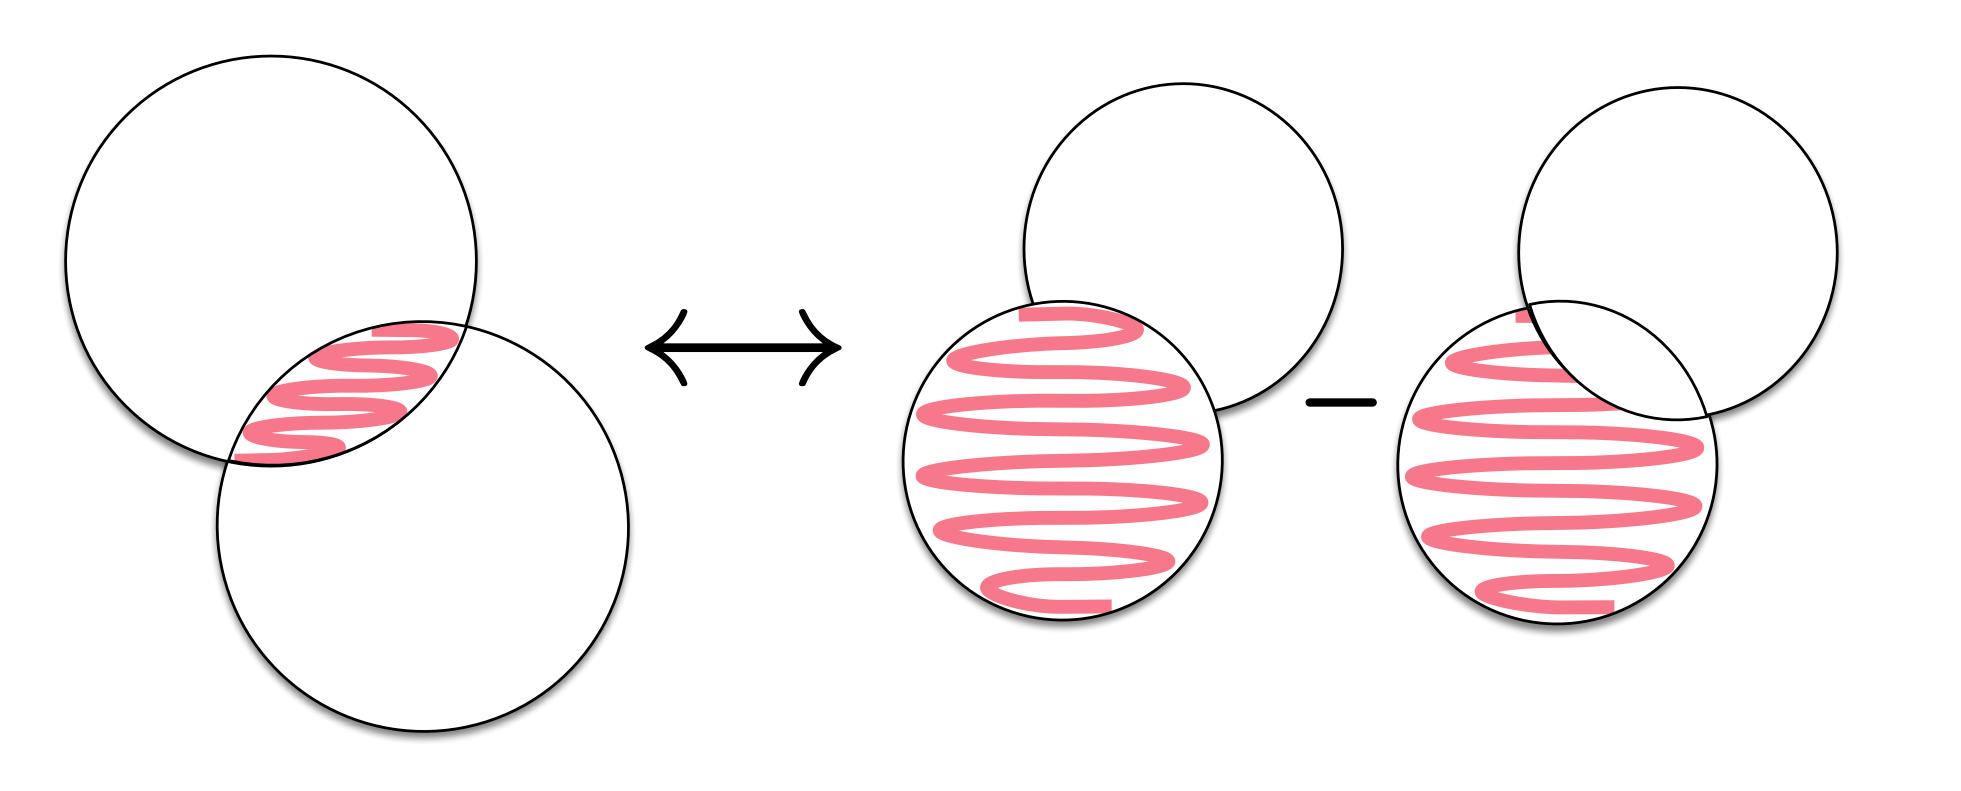
\includegraphics[width=12cm]{images/intersection1.png}
\caption{Venn-Diagram showing the definition of Intersection in terms of Set Difference}
\end{figure}
        
    \vspace{0.1in}
    
     \textbf{Part 4} \\
    Explain the difference between DRC and TRC.
    
    \vspace{0.1in}
        \solution \\
In Tuple Relational Calculus (TRC), the variables typically range over tuples, i.e. they directly represent tuples. On the other hand, in Domain Relational Calculus (DRC), the variables range over domain elements, i.e. field values. In TRC, tuples are semantically equivalent to variables, i.e. field referencing can be used to select tuple parts. On the other hand, in DRC, formal variables are explicit and have to be defined.
    \vspace{0.1in}
    
    
\end{homeworkProblem}   

\begin{homeworkProblem}

\textbf{Part 1} \\

The names of the seas that are deeper than 3000 mt and into which at least one river finally flows.

\vspace{0.1in}
    \solution \\
      
    $<name> \mid \exists depth, rname, river, lake, sea, length, sLong, sLat, mount, sAlt, estLong, estLat \\
    Sea(name, depth) \wedge  \\ River(rname, river, lake, sea, length, sLong, sLat, mount, sAlt, estLong, estLat) \wedge \\ depth > 3000 \wedge sea = name$ 
    \vspace{0.1in}
    
\textbf{Part 2} \\
The names of the groups of islands that consist only of islands that are neither 'volcanic' nor
'coral'.

 \vspace{0.1in}
    \solution \\ \\    
   %SOLUTION
   $<islands> \mid \exists name, area, height, type, long, lat \\
Island(name, islands, area, height, type, long, lat) \wedge \\
type \notin \{volcanic, coral\} \wedge islands \neq \emptyset  $
    \vspace{0.1in}    

\textbf{Part 3} \\
The name of the mountain, the name of the mountains where it belongs to and the name of
the country where the mountain is located for each mountain that is located on an island
that is of type 'coral'.

 
 \vspace{0.1in} 
     \solution \\ \\ 
     %SOLUTION   
     $<moiMountain, mMountains, gmCountry> \mid \exists \\ moiIsland, mHeight, mType, mLong, mLat, \\ iIslands, iArea, iHeight, iType, iLong, iLat, gmProvince \\
mountainOnIsland(moiMountain, moiIsland) \wedge \\ Mountain(moiMountain, mMountains, mHeight, mType, mLong, mLat) \wedge \\ geo\_Mountain(moiMountain, gmCountry, gmProvince)  \wedge \\
Island(moiIsland, iIslands, iArea, iHeight, iType, iLong, iLat) \wedge iType \neq "coral" $

     \vspace{0.1in}

    
\textbf{Part 4} \\
Give the name and country name of all cities with a population higher than 500,000.

 \vspace{0.1in} 
     \solution \\ \\    
    %SOLUTION
   $<cName, coName> \mid \exists cCountry, cProvince, cPopulation, cLong, cLat, \\
   coCapital, coProvince, coArea, coPopulation \\
City(cName, cCountry, cProvince, cPopulation, cLong, cLat)  \wedge \\
Country(cCountry, coName, coCapital, coProvince, coArea, coPopulation) \wedge \\
cPopulation > 500000 $
 
    \vspace{0.1in}
        
\end{homeworkProblem}

\begin{homeworkProblem}
Suppose you have a file of 15,000 pages and eight buffer pages and you are sorting it using general
(external) merge-sort. Please answer the following questions: \\

\textbf{Part 1} \\
How many runs will you produce? Remark: When a file is sorted, in intermediate steps
subfiles are created. Each sorted subfile is called a run. See also slide 35 in Chapter 2.
 \textbf{Note: Detailed solution of Q3 is produced in \textit{Figures 2, 3 and 4.}}
 
 \vspace{0.1in} 
     \solution \\
     %SOLUTION
     \textbf{2189} runs will be produced   
     \vspace{0.1in}
     
 \textbf{Part 2} \\
How many passes will it take to sort the file completely?
 
 \vspace{0.1in} 
     \solution \\ 
    It will take \textbf{5} passes   
     \vspace{0.1in}
     
 \textbf{Part 3} \\
How many buffer pages do you need at least to sort the file in two passes? 

 \vspace{0.1in} 
     \solution \\
     With \textbf{123} buffers, you can sort the file in two passes 
     \vspace{0.1in}
 
 \textbf{Part 4} \\
How many runs and passes would a Two-Way-Sort algorithm take?
 
 \vspace{0.1in} 
     \solution \\
     %SOLUTION
     Two-Way Sort Algorithm will take \textbf{30004} runs and \textbf{15} passes   
     \vspace{0.1in}   
     
\begin{figure}[h]
\centering
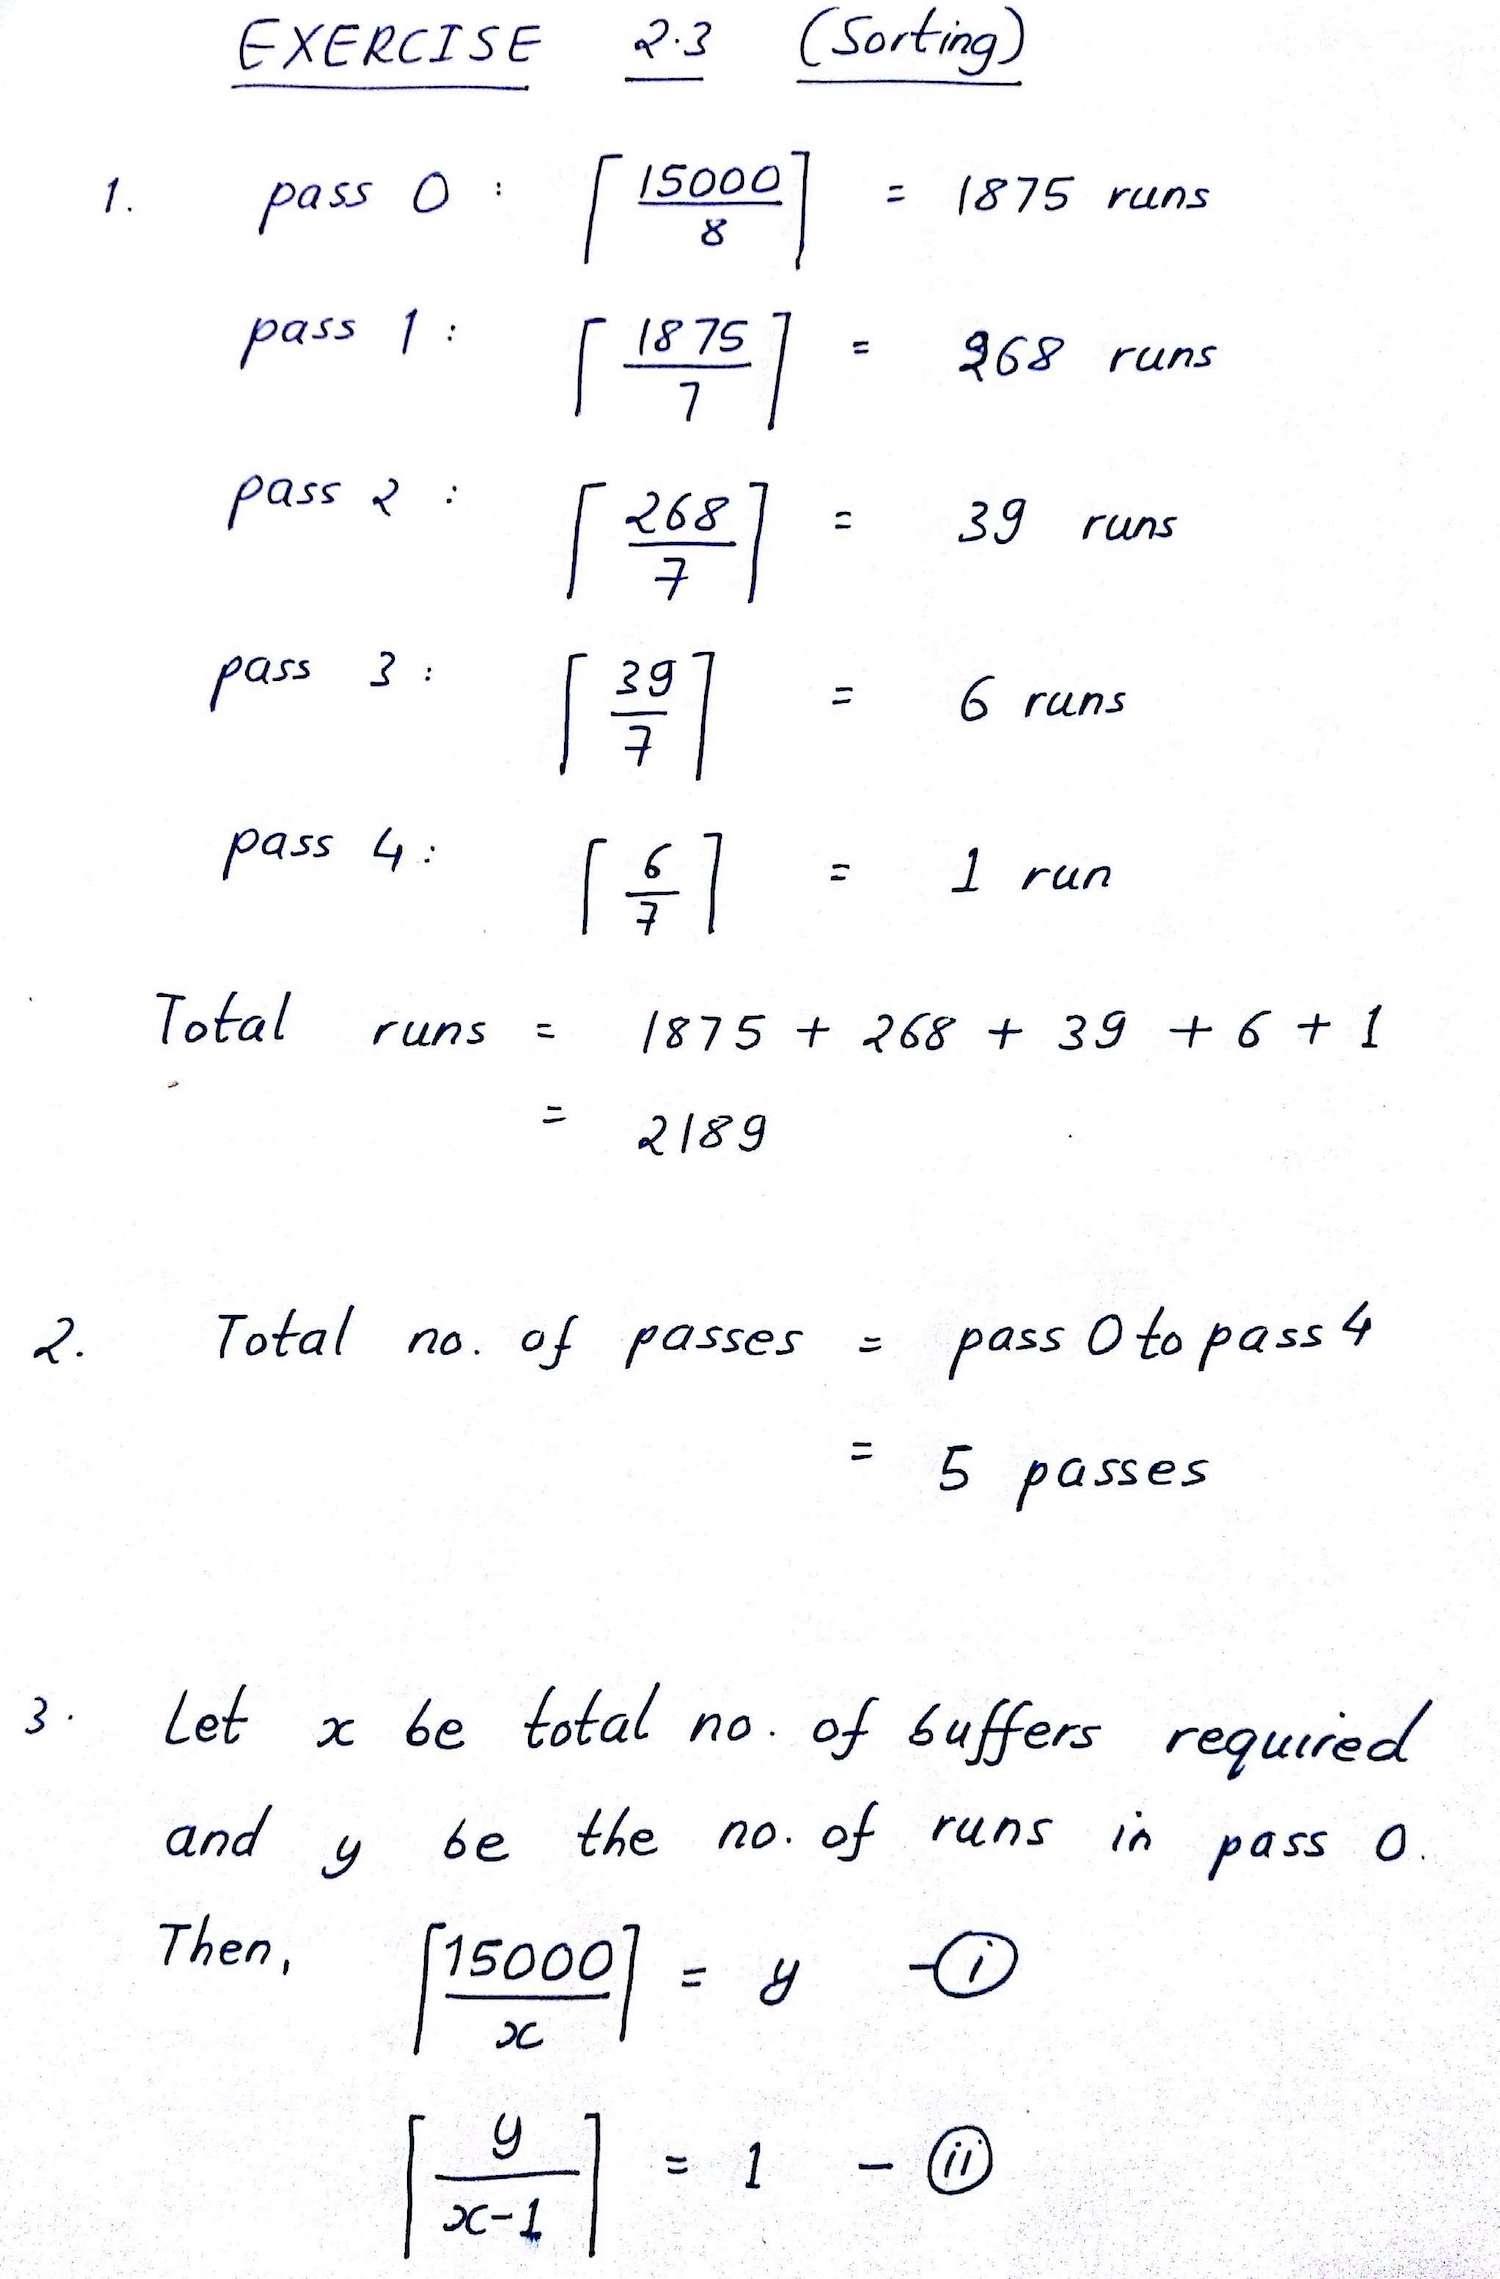
\includegraphics[width=12cm]{images/sol31.jpg}
\caption{Paper-based Solution for Question 3-1}
\end{figure} 

\begin{figure}[h]
\centering
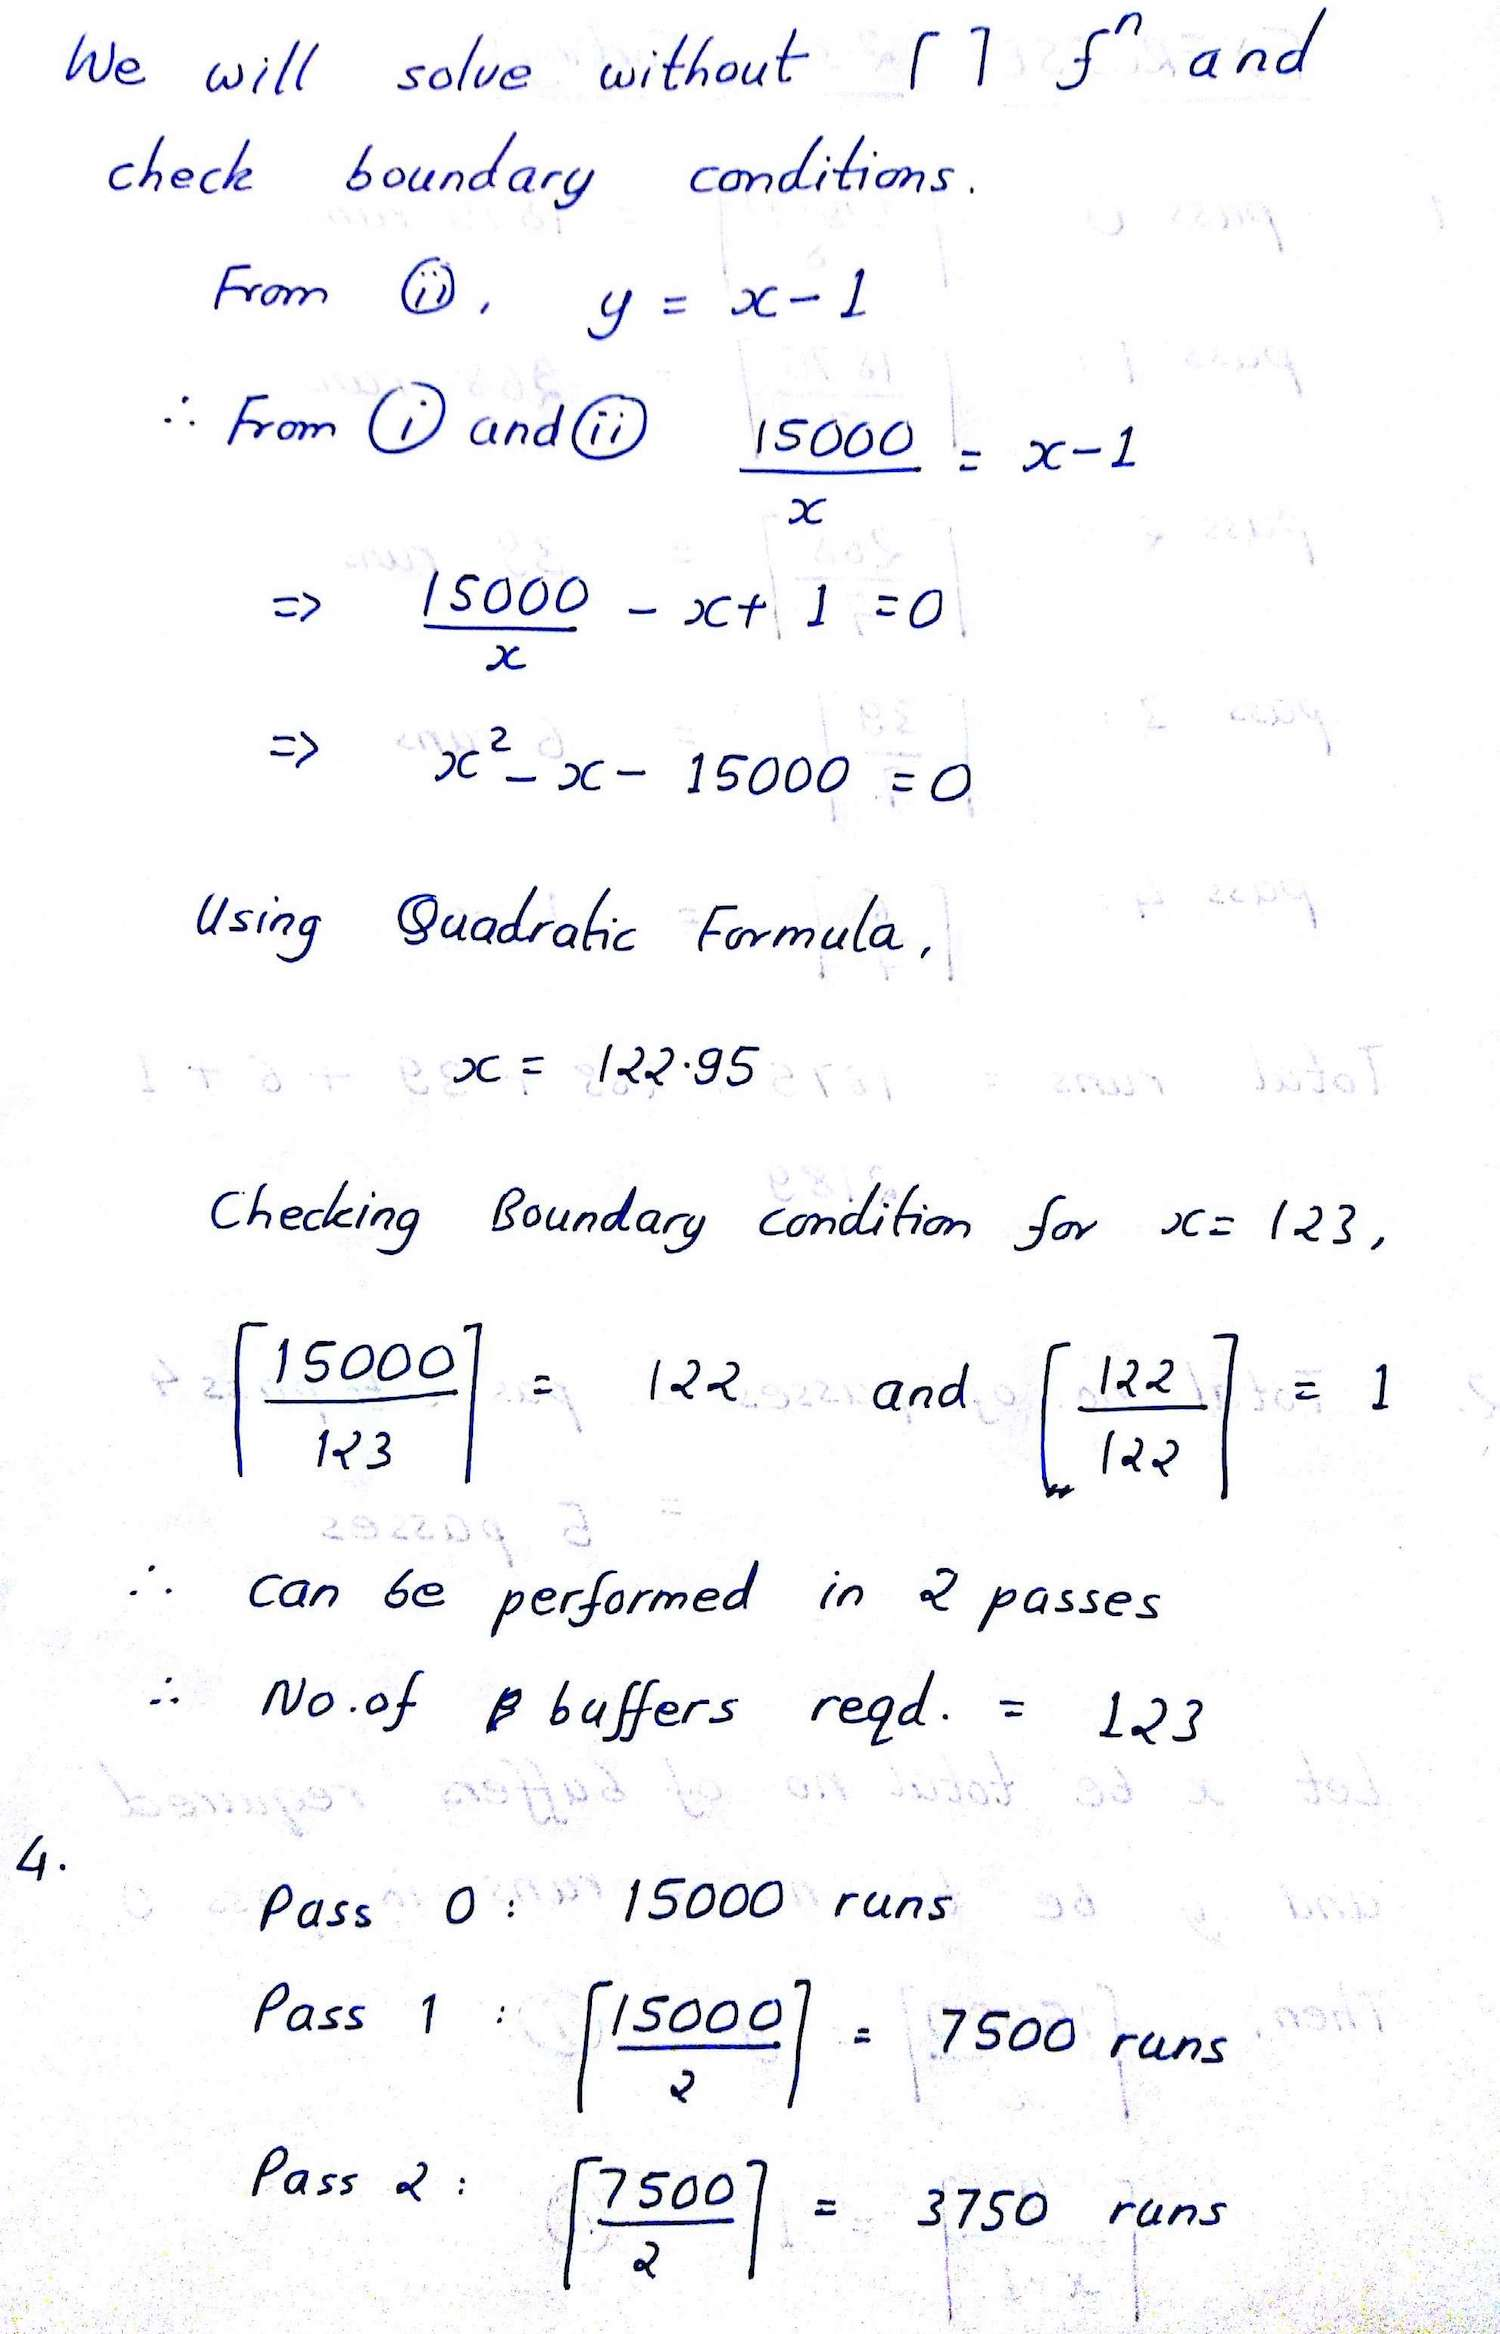
\includegraphics[width=12cm]{images/sol32.jpg}
\caption{Paper-based Solution for Question 3-2}
\end{figure} 

\begin{figure}[h]
\centering
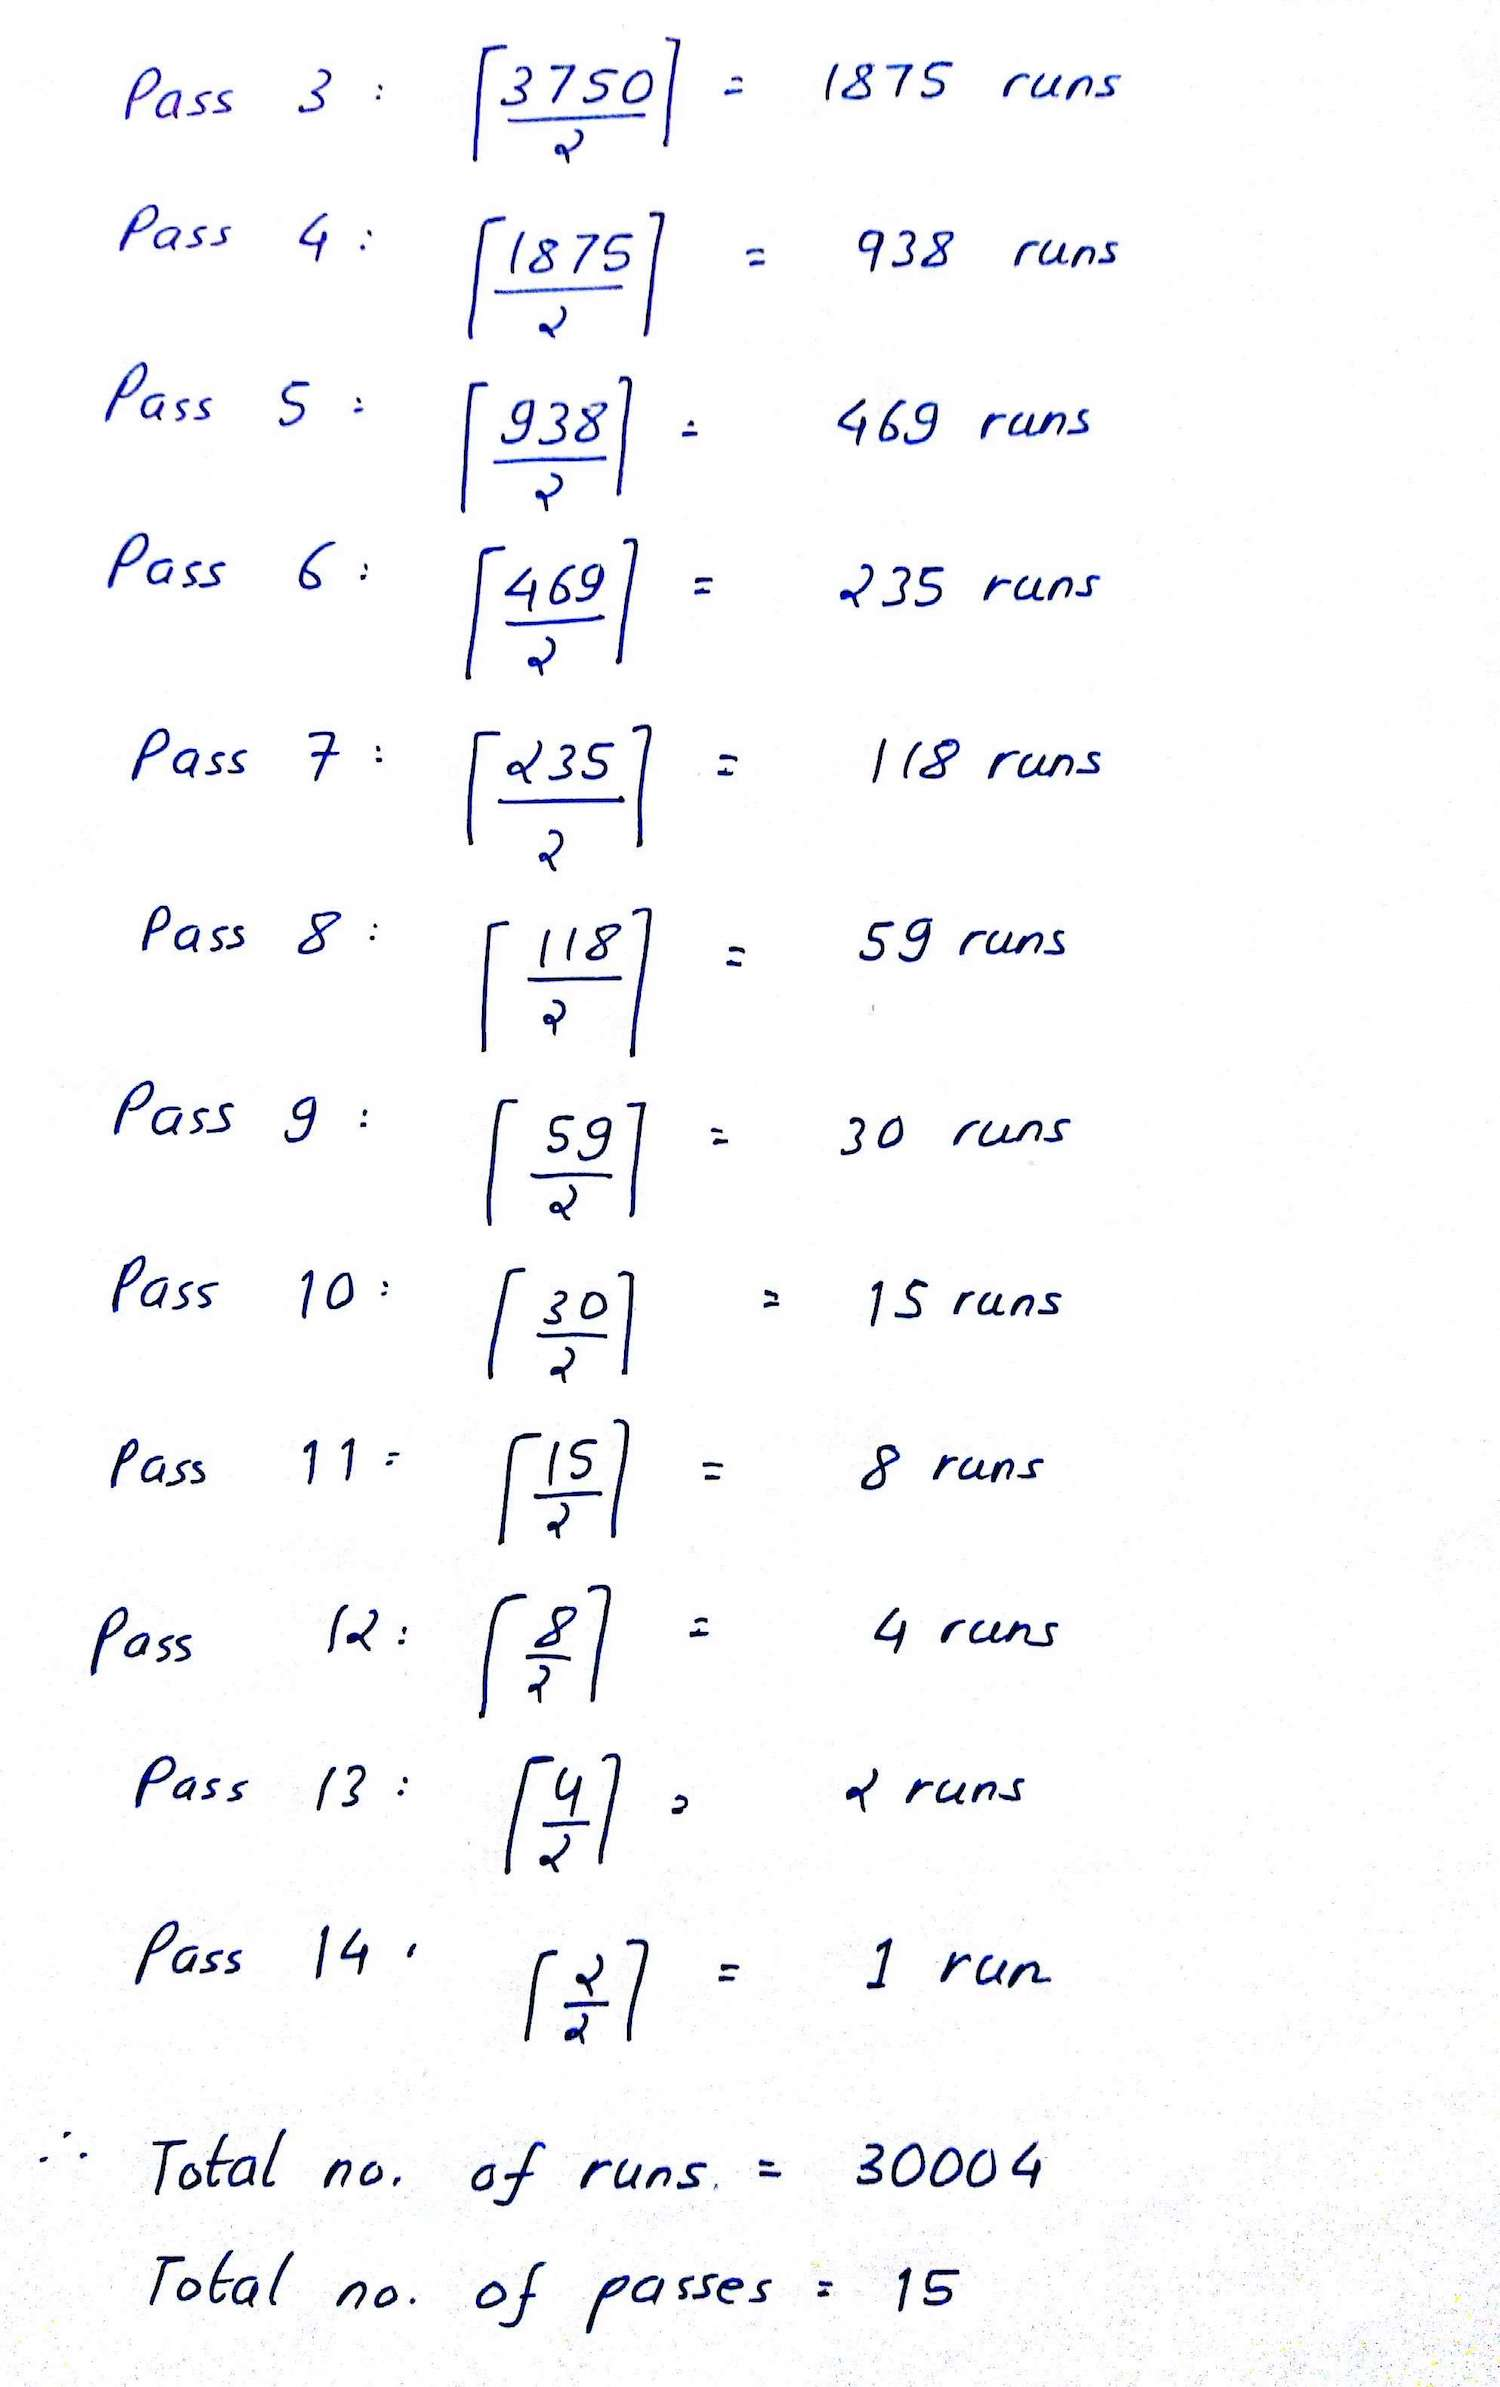
\includegraphics[width=12cm]{images/sol33.jpg}
\caption{Paper-based Solution for Question 3-3}
\end{figure} 

\end{homeworkProblem}

\begin{homeworkProblem}

\textbf{Part 1} \\
Calculate the I/O requirements of a simple nested loop join
 
 \vspace{0.1in} 
     \solution \\ \\ 
     %SOLUTION 
     In the expression below, M and N are the number of pages in the relations Album and Track respectively, $p_M$ and $p_N$ are the number of tuples in each page of the relations. \\
     
     \textbf{M as outer and N as inner relation} \\
     \textbf{Tuple-by-Tuple Simple Nested Loop Join} \\
     $M +  p_M \times M \times N$ \\
     $= 10000 + 100 \times 10000 \times 200000$ \\
     $ = 200000010000 $
          
    \vspace{0.1in}
     \textbf{Page-by-Page Simple Nested Loop Join} \\
     $M + M \times N$ \\
     $= 10000 + 10000 \times 200000$ \\
     $ = 2000010000 $
     
      \vspace{0.1in}
     \textbf{N as outer and M as inner relation} \\
     \textbf{Tuple-by-Tuple Simple Nested Loop Join} \\
     $N +  p_N \times N \times M$ \\
     $= 200000 + 80 \times 200000 \times 10000$ \\
     $ = 160000200000 $
          
    \vspace{0.1in}
     \textbf{Page-by-Page Simple Nested Loop Join} \\
     $M + M \times N$ \\
     $= 200000 + 200000 \times 10000$ \\
     $ = 2000200000 $
     \vspace{0.1in}
     
 \textbf{Part 2} \\
Calculate the I/O requirements of a block nested loop join
 
\vspace{0.1in} 
     \solution \\ \\ 
     %SOLUTION
     Block nested join for 16 buffers: \\
     
      \textbf{M as outer and N as inner relation} \\
     $ 10000 + \lceil \frac{10000}{14} \rceil \times 200000$
     $ = 143010000 $   
     \vspace{0.1in}
     
      \textbf{N as outer and M as inner relation} \\
      $ 200000 + \lceil \frac{200000}{14} \rceil \times 10000$
     $ = 143060000 $   
     \vspace{0.1in}
     
 \textbf{Part 3} \\
Explain the differences between the two algorithms. What are the similarities and differences? How does the block nested loop join reduce I/O costs?
 
 \vspace{0.1in} 
     \solution \\ \\ 
     %SOLUTION
     Tuple-at-a-time Simple Nested Loop Join scans outer relation and then for each tuple, it scans the entire inner relation. On the other hand, the page-at-a-time Simple Nested Loop Join will load the outer relation page-by-page, and then the inner relation for each page. The Block Nested Loop Join, on the other hand, scans entire inner relation for each block of pages in the outer relation. Therefore, the I/O cost of Block Nested Loop Join is lower than cost of both the Simple Nested Loop Joins. 
Moreover, the other important difference is number of buffer pages used in the algorithms. Both tuple-at-a-time nested loop and page-at-time nested loop join use 3 buffer pages to perform the join operation. 1 page as input buffer to scan outer relation,1 page as input buffer to scan inner relation  and 1 page as output buffer. Totally, 3 pages are needed for simple nested loop join. However, block nested loop join uses 1 page as input buffer to scan inner relation S and 1 page as output buffer. The other remaining buffer pages are used to load the blocks of the outer relation R. In this case, 1 buffer page is used as input buffer to scan inner relation  and 1 page as output buffer. Remaining 14 buffer pages are used to block outer relation . As seen, block nested loop join uses entire available buffer pages in the algorithm that means more efficient usage of buffer pages and causing performance increases and decreasing I/O cost. 

The similarities can be indicated as outer-inner relation usage, buffer usage and loop operations in the algorithms. 

     \vspace{0.1in}
     
\end{homeworkProblem}
     
\begin{homeworkProblem}
Given is a relation with 50.000 records. Each page for a node in a B+ tree can hold 20 pointers
to records or pages. A data page can store 20 records. \\

 \textbf{Part 1} \\
Assume that each node is 70 \% full. What is the height of the B+-tree? 

 \vspace{0.1in} 
     \solution \\ \\ 
     %SOLUTION  
     Given that the B+Tree can hold 20 pointers to pages. However, the B+ Tree has 70\% occupancy. Therefore, number of effective pointers to pages that the tree can hold,
     \begin{center} $ \implies 0.7 \times 20 = 14$ \end{center} 
Our B+ Tree can now be represented as Table 1

\begin{table}[]
\centering
\begin{tabular}{|l|l|l|l|}
\hline
Level    & Node & Entries & No. of Pointers \\ \hline
0 (Root) & 1    & 13      & 14              \\ \hline
1        & 14   & 182     & 196             \\ \hline
2        & 196  & 2548    & 2744         \\ \hline  
\end{tabular}
\caption{Different Levels of the B+ Tree}
\label{B+ Tree}
\end{table}

We have 2744 addresses in Level 2 already, which is more than 2500 pointers to pages required in the relations. \\
Therefore, the B-Tree has a depth of \textbf{3}.
Our B+ Tree has a depth of \textbf{3}
 \vspace{0.1in}
     
 \textbf{Part 2} \\
What are the I/O costs for an equality selection on a non-key attribute for the following
cases?

\begin{enumerate}[label = (\alph*)]
\item with a clustered B+-tree of height 3 (matching records are located in one page);
 
 \vspace{0.1in} 
     \solution \\ \\ 
     %SOLUTION
     The clustered index will guide the search, and after the end of the B+ tree traversal, we will need to input the correct page which contains our desired result. Therefore, total I/O is for the tree traversal and retrieving the correct page, i.e. 3 I/Os + 1 I/O = 4.
     Hence, total number of I/Os = \textbf{4} I/Os
     \vspace{0.1in}
     
\item without any index, nor is the file sorted on the attribute occurring in selection;

\vspace{0.1in} 
     \solution \\ \\ 
     %SOLUTION 
     Total number of pages at the leaf node = 2500
    If we consider that all pages need to be scanned, then the I/O costs will be \textbf{2500} I/Os. \\
    However, assuming, on an average that half the total number of pages need to be searched to find the equality results, it gives a total of 1250 I/Os.
          
     \vspace{0.1in}
     
\item with an unclustered B+-tree index of height 4, and there are 2 matching records;

\vspace{0.1in} 
     \solution \\ \\ 
     4 I/Os to traverse the tree + 2 I/Os to retrieve the matching records = \textbf{6} I/Os 
     \vspace{0.1in}

\item with an unclustered B+-tree of height 5 and three tenth of the records match the
selection.

\vspace{0.1in} 
\solution \\ \\ 
     %SOLUTION
     No. of matching records = $\frac{3}{10} \times 50000 = 15000$ records \\
     In the worst case, we need to do 15000 page I/Os, one for each record. Plus the I/Os for traversing the tree. Therefore, a total of 15000 I/Os + 5 I/Os = \textbf{15005} I/Os.   
     \vspace{0.1in}

\end{enumerate}
\end{homeworkProblem}

\end{document}
\documentclass[12pt]{article}

\usepackage{fancyhdr}
\usepackage{extramarks}
\usepackage{amsmath}
\usepackage{amsthm}
\usepackage{amsfonts}
\usepackage{tikz}
\usepackage[plain]{algorithm}
\usepackage{algpseudocode}
\usepackage[export]{adjustbox}
\usepackage[latin1]{inputenc}           %For German characters
\usepackage{enumitem}               %For changing enumeration character
\usepackage{listings}               %For code
\usepackage{csquotes}
\usepackage{graphicx}               %For graphics e.g, images

\usetikzlibrary{automata,positioning}

%
% Basic Document Settings
%

\topmargin=-0.45in
\evensidemargin=0in
\oddsidemargin=0in
\textwidth=6.5in
\textheight=9.0in
\headsep=0.25in

\linespread{1.1}

\pagestyle{fancy}
\lhead{\hmwkAuthorName}
\chead{\hmwkClass\ : \hmwkTitle}
\rhead{\firstxmark}
\lfoot{\lastxmark}
\cfoot{\thepage}

\renewcommand\headrulewidth{0.4pt}
\renewcommand\footrulewidth{0.4pt}

\setlength\parindent{0pt}

%
% Create Problem Sections
%

\newcommand{\enterProblemHeader}[1]{
    \nobreak\extramarks{}{Problem \arabic{#1} continued on next page\ldots}\nobreak{}
    \nobreak\extramarks{Problem \arabic{#1} (continued)}{Problem \arabic{#1} continued on next page\ldots}\nobreak{}
}

\newcommand{\exitProblemHeader}[1]{
    \nobreak\extramarks{Problem \arabic{#1} (continued)}{Problem \arabic{#1} continued on next page\ldots}\nobreak{}
    \stepcounter{#1}
    \nobreak\extramarks{Problem \arabic{#1}}{}\nobreak{}
}

\setcounter{secnumdepth}{0}
\newcounter{partCounter}
\newcounter{homeworkProblemCounter}
\setcounter{homeworkProblemCounter}{1}
\nobreak\extramarks{Problem \arabic{homeworkProblemCounter}}{}\nobreak{}

%
% Homework Problem Environment
%
% This environment takes an optional argument. When given, it will adjust the
% problem counter. This is useful for when the problems given for your
% assignment aren't sequential. See the last 3 problems of this template for an
% example.
%
\newenvironment{homeworkProblem}[1][-1]{
    \ifnum#1>0
        \setcounter{homeworkProblemCounter}{#1}
    \fi
    \section{Problem \arabic{homeworkProblemCounter}}
    \setcounter{partCounter}{1}
    \enterProblemHeader{homeworkProblemCounter}
}{
    \exitProblemHeader{homeworkProblemCounter}
}

%
% Homework Details
%   - Title
%   - Due date
%   - Class
%   - Section/Time
%   - Instructor
%   - Author
%

\newcommand{\hmwkTitle}{Assignment\ \#2}
\newcommand{\hmwkDueDate}{November 15, 2016}
\newcommand{\hmwkClass}{Implementation of Databases}
\newcommand{\hmwkAuthorName}{Sanchit Alekh}
\newcommand{\hmwkClassTime}{MSc. Software Systems Engineering}
\newcommand{\hmwkClassInstructor}{Universitätsprofessor Dr. rer. pol. Matthias Jarke}
\newcommand{\hmwkClassInstructors}{Dr. rer. nat. Christoph Quix}

%
% Title Page
%



\title{
   \begin{center}
   \vspace*{-20mm}
   
\includegraphics[width=0.4\textwidth, right]{images/rwth_logo.png}
   \\
   \vspace*{3cm}
    \textmd{\textbf{\hmwkClass}}\\
    \textmd{\textbf{\hmwkTitle}}\\
    \normalsize\vspace{0.1in}\small{Due\ on\ \hmwkDueDate } \\
    \vspace{0.1in}\large{\textit{\hmwkClassInstructor}} \\
    \vspace{0.1in}\large{\textit{\hmwkClassInstructors}} \\
    \vspace{3in}
     \textbf{Submitted by:} \\
     \vspace{0.25in}
    \large{Sanchit Alekh, Idil Esen Zülfikar, Nihal Hegde} \\
    %\author{\textbf{\hmwkAuthorName}}
    \vspace{0.1in} \large{\textit{\hmwkClassTime}} \\
    %\vspace{0.1in} \large{\textit{Matrikelnummer : 359831}}
    \end{center}
    }


\date{}

\renewcommand{\part}[1]{\textbf{\large Part \Alph{partCounter}}\stepcounter{partCounter}\\}

%
% Various Helper Commands
%

% Useful for algorithms
\newcommand{\alg}[1]{\textsc{\bfseries \footnotesize #1}}

% For derivatives
\newcommand{\deriv}[1]{\frac{\mathrm{d}}{\mathrm{d}x} (#1)}

% For partial derivatives
\newcommand{\pderiv}[2]{\frac{\partial}{\partial #1} (#2)}

% Integral dx
\newcommand{\dx}{\mathrm{d}x}

% Alias for the Solution section header
\newcommand{\solution}{\textbf{\large Solution}}

% Probability commands: Expectation, Variance, Covariance, Bias
\newcommand{\E}{\mathrm{E}}
\newcommand{\Var}{\mathrm{Var}}
\newcommand{\Cov}{\mathrm{Cov}}
\newcommand{\Bias}{\mathrm{Bias}}

\begin{document}

\maketitle

\pagebreak

\begin{homeworkProblem}
    
    \textbf{Part 1} \\
    Variants of relational algebra are used internally in DBMS to represent queries and query evaluation plans. Please explain, why relational algebra is suitable for this?
    
    \vspace{0.1in}
    \solution \\
    One of the most desirable properties of Relational Algebra is that queries are composed using a collection of operators, and every operator accepts one or two relation instances as arguments and returns a relation instance as the result. This property makes extremely easy and efficient to compose operators to form a complex query. A relational algebra expression can be recursively defined to be a relation, a unary algebra operator applied to a single expression, or a binary algebra operator applied to two expressions. 
This procedural nature of relational algebra is the main reason why it is used internally in DBMS to represent queries and evaluation plans. The approach allows us to think of an algebra expression as an imperative execution plan for a declarative SQL query. It can be used for evaluating a query, and relational systems in fact use algebra expressions to represent query evaluation plans.
        
    \vspace{0.1in}
    
    \textbf{Part 2} \\
    What does \enquote{relational completeness} mean (in your own words, please)? Show that SQL is
relationally complete by enumerating SQL constructs corresponding to selection, projection,
cartesian product, union, and difference.
    
    \vspace{0.1in}
    \solution \\
    \enquote{Relational Completeness} of a query methodology means that each and every query that can be expressed using that methodology, can also be expressed as a relational algebra query. In this case, SQL is referred to as \enquote*{Relationally Complete} because every legal construct in SQL can be expressed as a Relational Algebra query.
        
These are the examples of Relational Algebra expressions and their equivalent expressions in SQL. The following examples are derived from the \textit{Mondial} database.

\begin{itemize}

\item \textbf{SELECTION} \\
Relational Algebra: $ \sigma_{Area > 650} (Island)$ \\
SQL:  \textit{Select * From Island Where Area $>$ 650;}

\item \textbf{PROJECTION} \\
Relational Algebra: $ \pi_{Name, Islands, Area, Height} (Island)$ \\
SQL: \textit{Select Name, Islands, Area, Height From Island;}

\item \textbf{CARTESIAN PRODUCT} \\
Relational Algebra:  $ Island \times islandIn$ \\
SQL: \textit{Select * From Island CROSS JOIN islandIn;}

\item \textbf{UNION} \\
Relational Algebra:  $ \pi_{name} (Desert) \cup \pi_{name} (geo\_Desert)$ \\
SQL: \textit{Select name From Desert or Select name From geo\_Desert}

\item \textbf{SET DIFFERENCE} \\
Relational Algebra: $ \pi_{name} (\sigma_{height > 5000} (Mountain)) - \pi_{name}( \sigma_{type > 'volcanic')} (Mountain) $ \\
SQL: \textit{Select name From Mountain where height $>$ 5000 MINUS Select name From Mountain where type='volcanic'}
\end{itemize}
        
    \vspace{0.1in}
        
     \textbf{Part 3} \\
    Explain how the intersection operator is used in relational algebra. What is important for
its usage? Is it omittable (i.e., could you express it by other operators)? If so, please give
the corresponding relational algebra.
    
    \vspace{0.1in}
    \solution \\
    The \enquote*{Intersection} operator is represented in Relational Algebra with the help of the $\cap$ symbol. Although it is not a fundamental set-operator, it is an extremely widely used operation, and it is helpful to define it separately. An example use of the intersection operator is as follows:
    
    \begin{center} $ \pi_{name} (Desert) \cap \pi_{name} (geo\_Desert) $ \end{center}
    
The important condition for using the \textit{Intersection} operator is that the two sets which have to be intersected must be \textit{union-compatible}. This follows from the fact that intersection is defined in terms of set difference.

Yes, Intersection is not a fundamental set-operator, and it can be expressed in terms of the set-difference operator. Therefore, it is omittable. A general expression for the intersection operator in terms of the set-difference operator is:

    \begin{center} $ A \cup B \leftrightarrow A \setminus ( A \setminus B) $ \end{center}
    
Therefore, the example Relational Algebra query illustrated above can be represented by the equivalent query without the use of set-intersection as follows:

    \begin{center} $ \pi_{name} (Desert) - (\pi_{name} (Desert) - \pi_{name} (geo\_Desert))$ \end{center}
    
\begin{figure}[h]
\centering
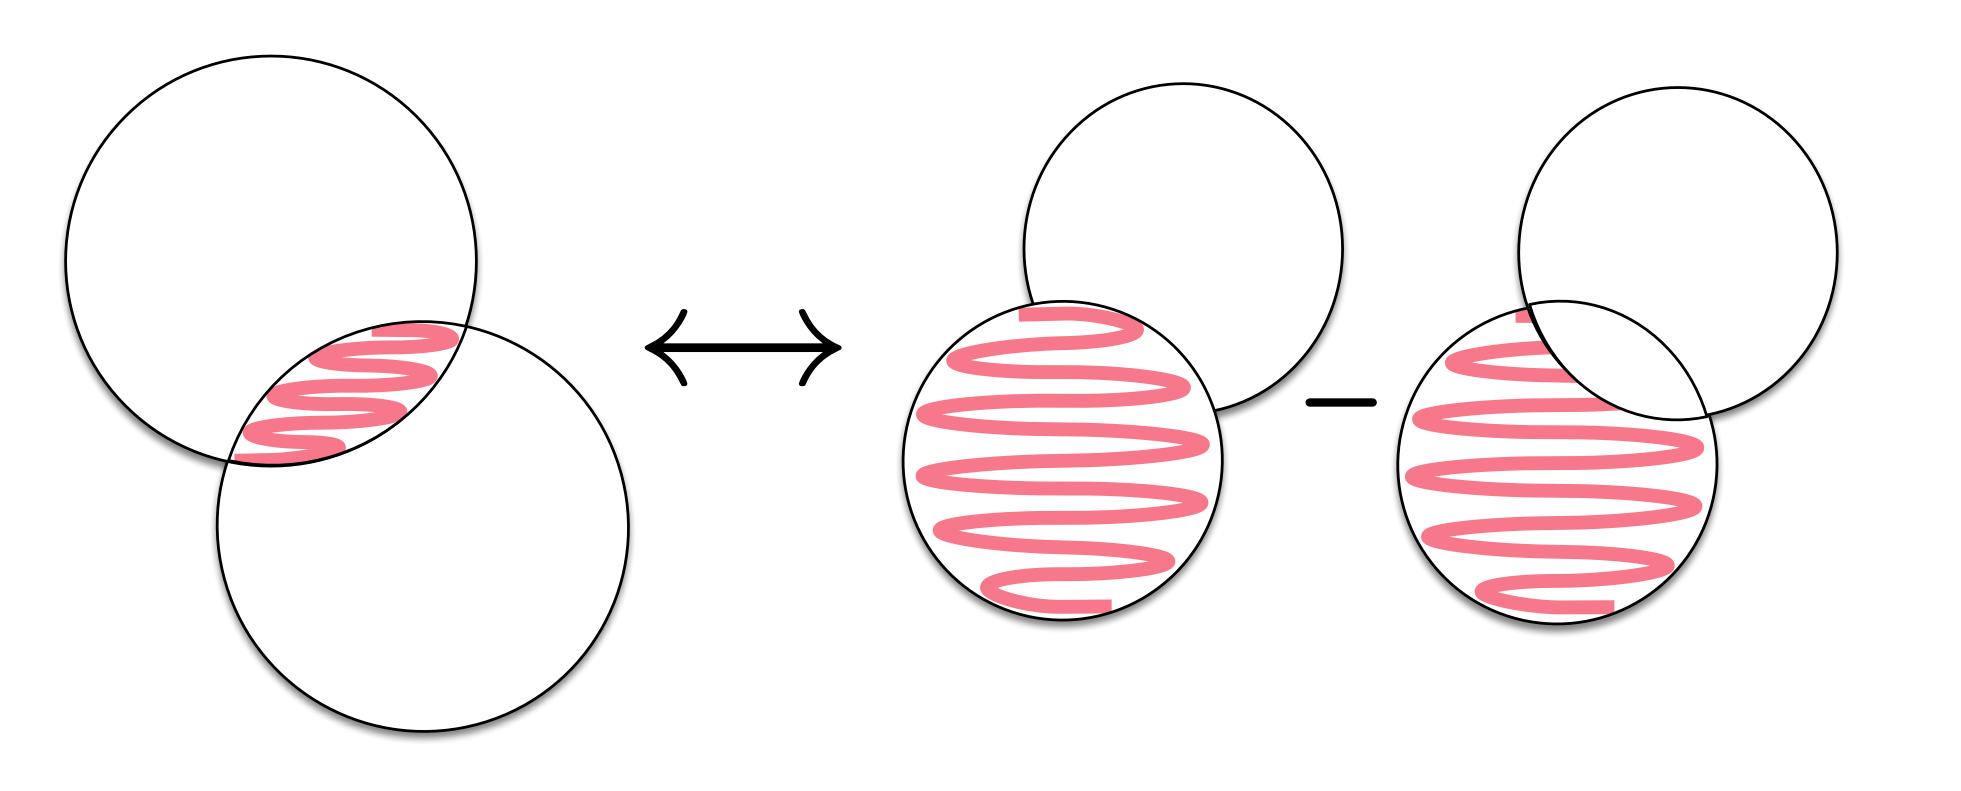
\includegraphics[width=12cm]{images/intersection1.png}
\caption{Venn-Diagram showing the definition of Intersection in terms of Set Difference}
\end{figure}
        
    \vspace{0.1in}
    
     \textbf{Part 4} \\
    Explain the difference between DRC and TRC.
    
    \vspace{0.1in}
        \solution \\
In Tuple Relational Calculus (TRC), the variables typically range over tuples, i.e. they directly represent tuples. On the other hand, in Domain Relational Calculus (DRC), the variables range over domain elements, i.e. field values. In TRC, tuples are semantically equivalent to variables, i.e. field referencing can be used to select tuple parts. On the other hand, in DRC, formal variables are explicit and have to be defined.
    \vspace{0.1in}
    
    
\end{homeworkProblem}   

\begin{homeworkProblem}

\textbf{Part 1} \\

The names of the seas that are deeper than 3000 mt and into which at least one river finally flows.

\vspace{0.1in}
    \solution \\
      
    $<name> \mid \exists depth, rname, river, lake, sea, length, sLong, sLat, mount, sAlt, estLong, estLat \\
    Sea(name, depth) \wedge  \\ River(rname, river, lake, sea, length, sLong, sLat, mount, sAlt, estLong, estLat) \wedge \\ depth > 3000 \wedge sea = name$ 
    \vspace{0.1in}
    
\textbf{Part 2} \\
The names of the groups of islands that consist only of islands that are neither 'volcanic' nor
'coral'.

 \vspace{0.1in}
    \solution \\ \\    
   %SOLUTION
   $<islands> \mid \exists name, area, height, type, long, lat \\
Island(name, islands, area, height, type, long, lat) \wedge \\
type \notin \{volcanic, coral\} \wedge islands \neq \emptyset  $
    \vspace{0.1in}    

\textbf{Part 3} \\
The name of the mountain, the name of the mountains where it belongs to and the name of
the country where the mountain is located for each mountain that is located on an island
that is of type 'coral'.

 
 \vspace{0.1in} 
     \solution \\ \\ 
     %SOLUTION   
     $<moiMountain, mMountains, gmCountry> \mid \exists \\ moiIsland, mHeight, mType, mLong, mLat, \\ iIslands, iArea, iHeight, iType, iLong, iLat, gmProvince \\
mountainOnIsland(moiMountain, moiIsland) \wedge \\ Mountain(moiMountain, mMountains, mHeight, mType, mLong, mLat) \wedge \\ geo\_Mountain(moiMountain, gmCountry, gmProvince)  \wedge \\
Island(moiIsland, iIslands, iArea, iHeight, iType, iLong, iLat) \wedge iType \neq "coral" $

     \vspace{0.1in}

    
\textbf{Part 4} \\
Give the name and country name of all cities with a population higher than 500,000.

 \vspace{0.1in} 
     \solution \\ \\    
    %SOLUTION
   $<cName, coName> \mid \exists cCountry, cProvince, cPopulation, cLong, cLat, \\
   coCapital, coProvince, coArea, coPopulation \\
City(cName, cCountry, cProvince, cPopulation, cLong, cLat)  \wedge \\
Country(cCountry, coName, coCapital, coProvince, coArea, coPopulation) \wedge \\
cPopulation > 500000 $
 
    \vspace{0.1in}
        
\end{homeworkProblem}

\begin{homeworkProblem}
Suppose you have a file of 15,000 pages and eight buffer pages and you are sorting it using general
(external) merge-sort. Please answer the following questions: \\

\textbf{Part 1} \\
How many runs will you produce? Remark: When a file is sorted, in intermediate steps
subfiles are created. Each sorted subfile is called a run. See also slide 35 in Chapter 2.
 \textbf{Note: Detailed solution of Q3 is produced in \textit{Figures 2, 3 and 4.}}
 
 \vspace{0.1in} 
     \solution \\
     %SOLUTION
     \textbf{2189} runs will be produced   
     \vspace{0.1in}
     
 \textbf{Part 2} \\
How many passes will it take to sort the file completely?
 
 \vspace{0.1in} 
     \solution \\ 
    It will take \textbf{5} passes   
     \vspace{0.1in}
     
 \textbf{Part 3} \\
How many buffer pages do you need at least to sort the file in two passes? 

 \vspace{0.1in} 
     \solution \\
     With \textbf{123} buffers, you can sort the file in two passes 
     \vspace{0.1in}
 
 \textbf{Part 4} \\
How many runs and passes would a Two-Way-Sort algorithm take?
 
 \vspace{0.1in} 
     \solution \\
     %SOLUTION
     Two-Way Sort Algorithm will take \textbf{30004} runs and \textbf{15} passes   
     \vspace{0.1in}   
     
\begin{figure}[h]
\centering
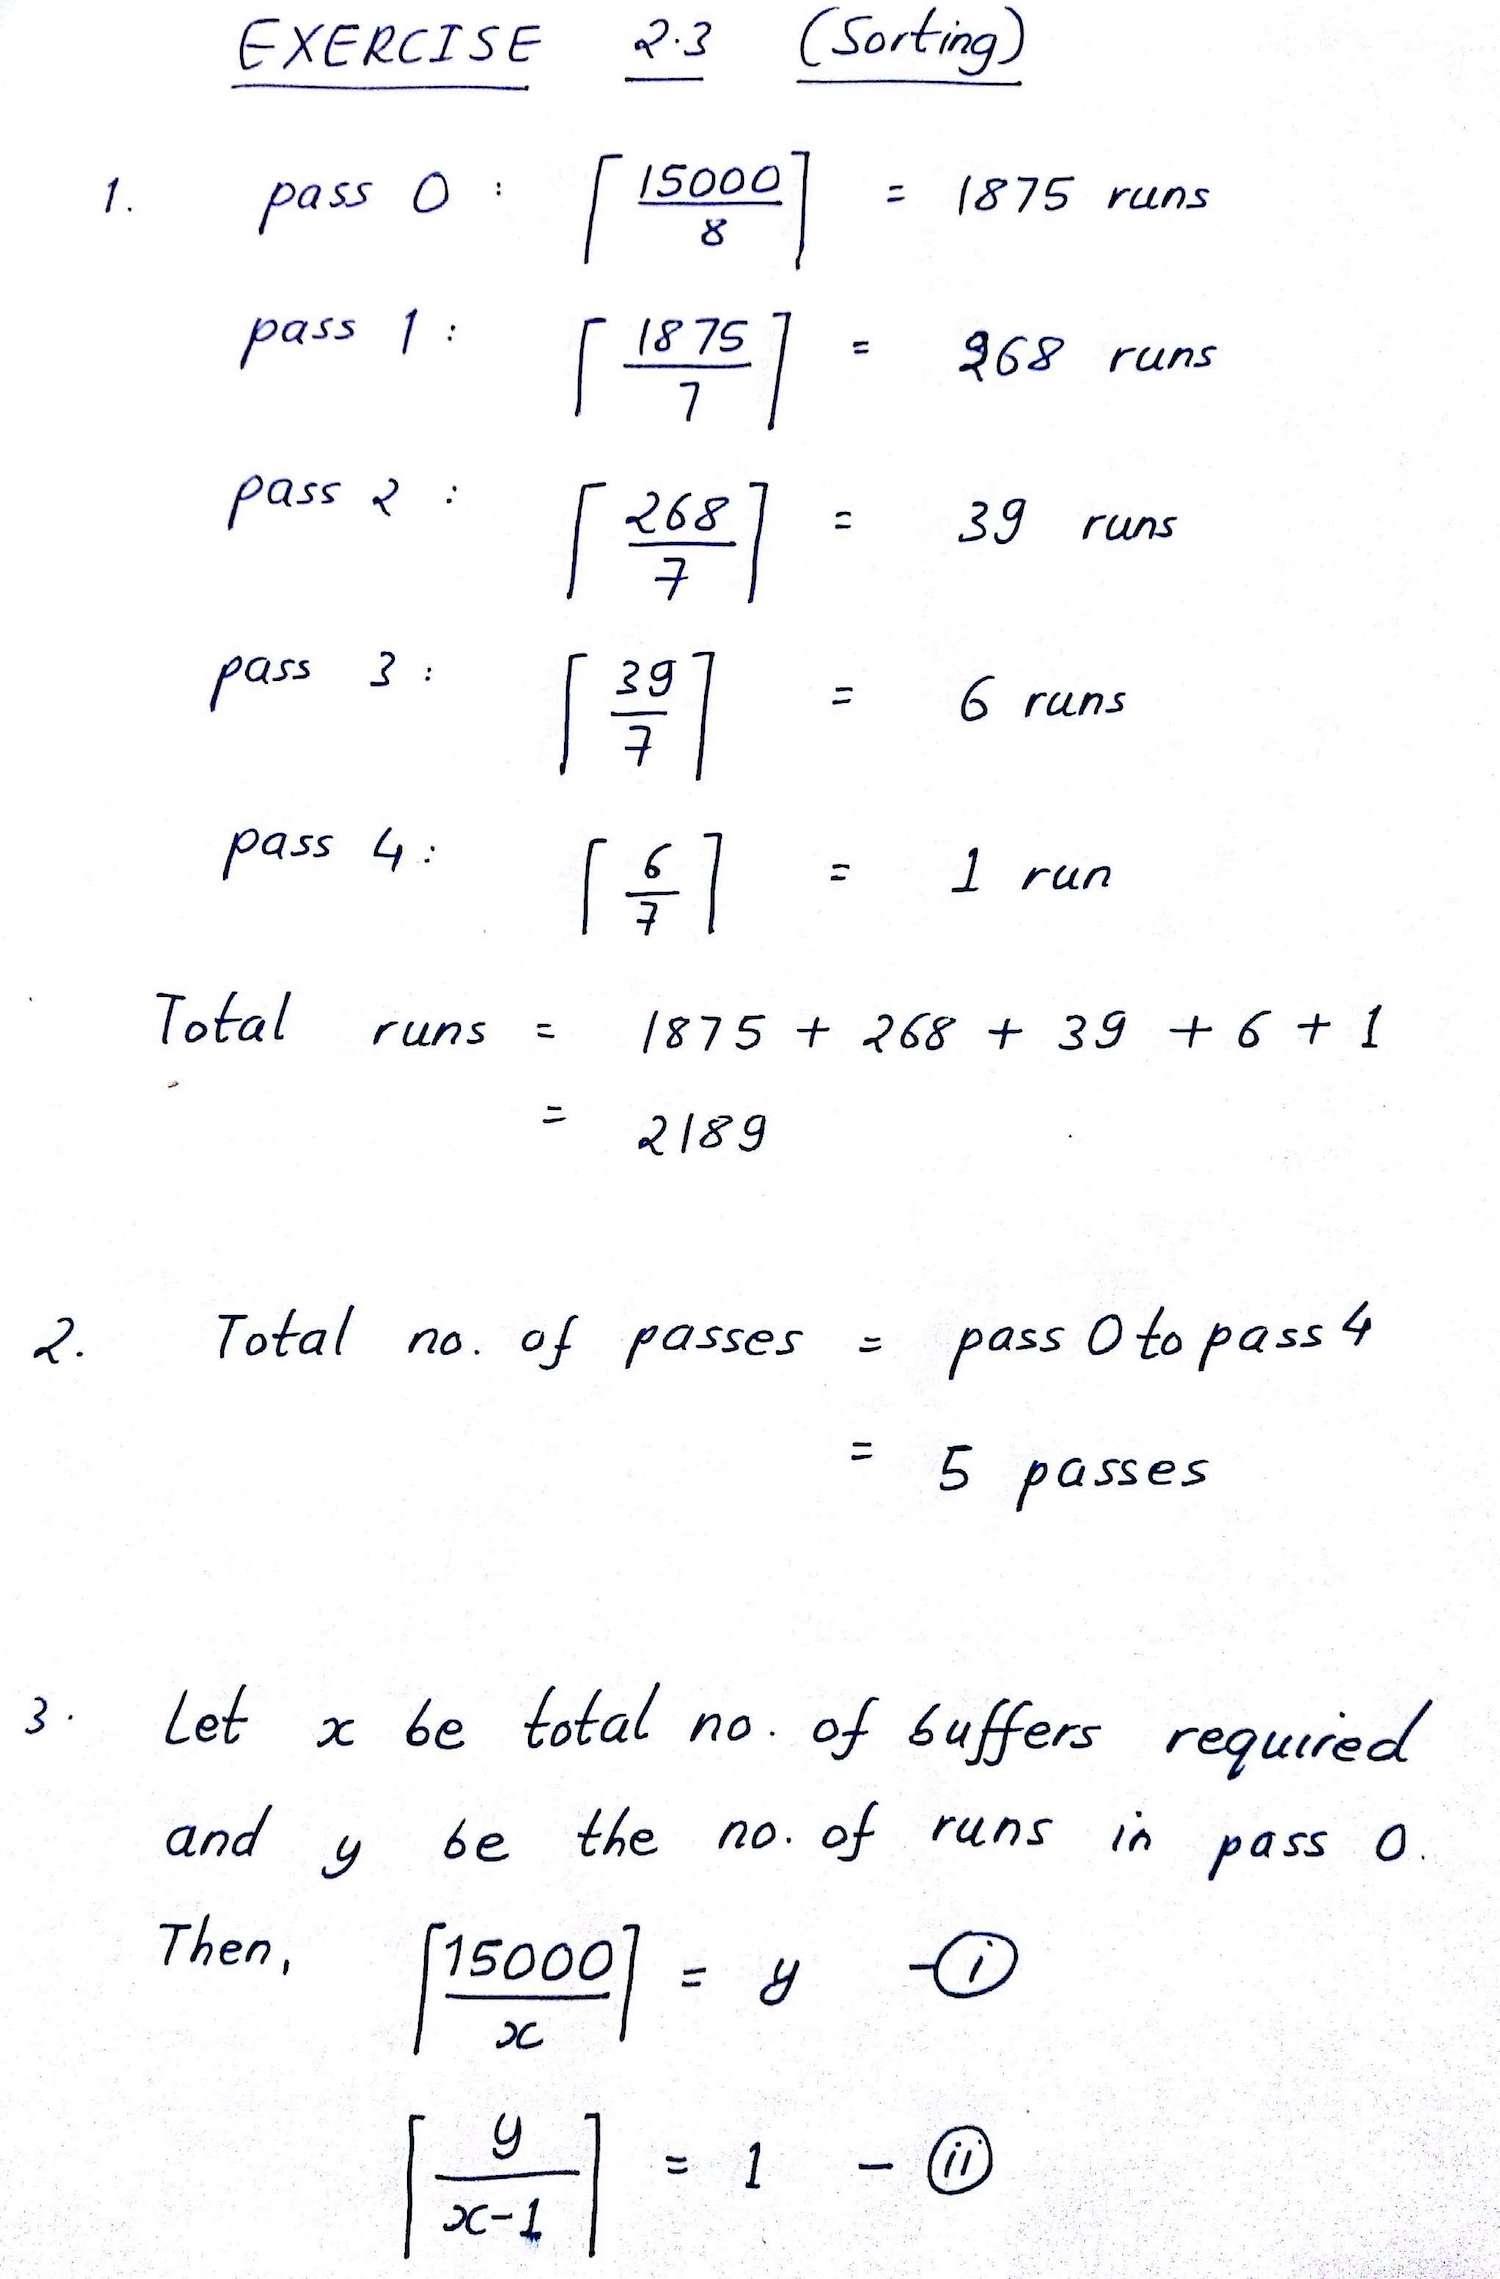
\includegraphics[width=12cm]{images/sol31.jpg}
\caption{Paper-based Solution for Question 3-1}
\end{figure} 

\begin{figure}[h]
\centering
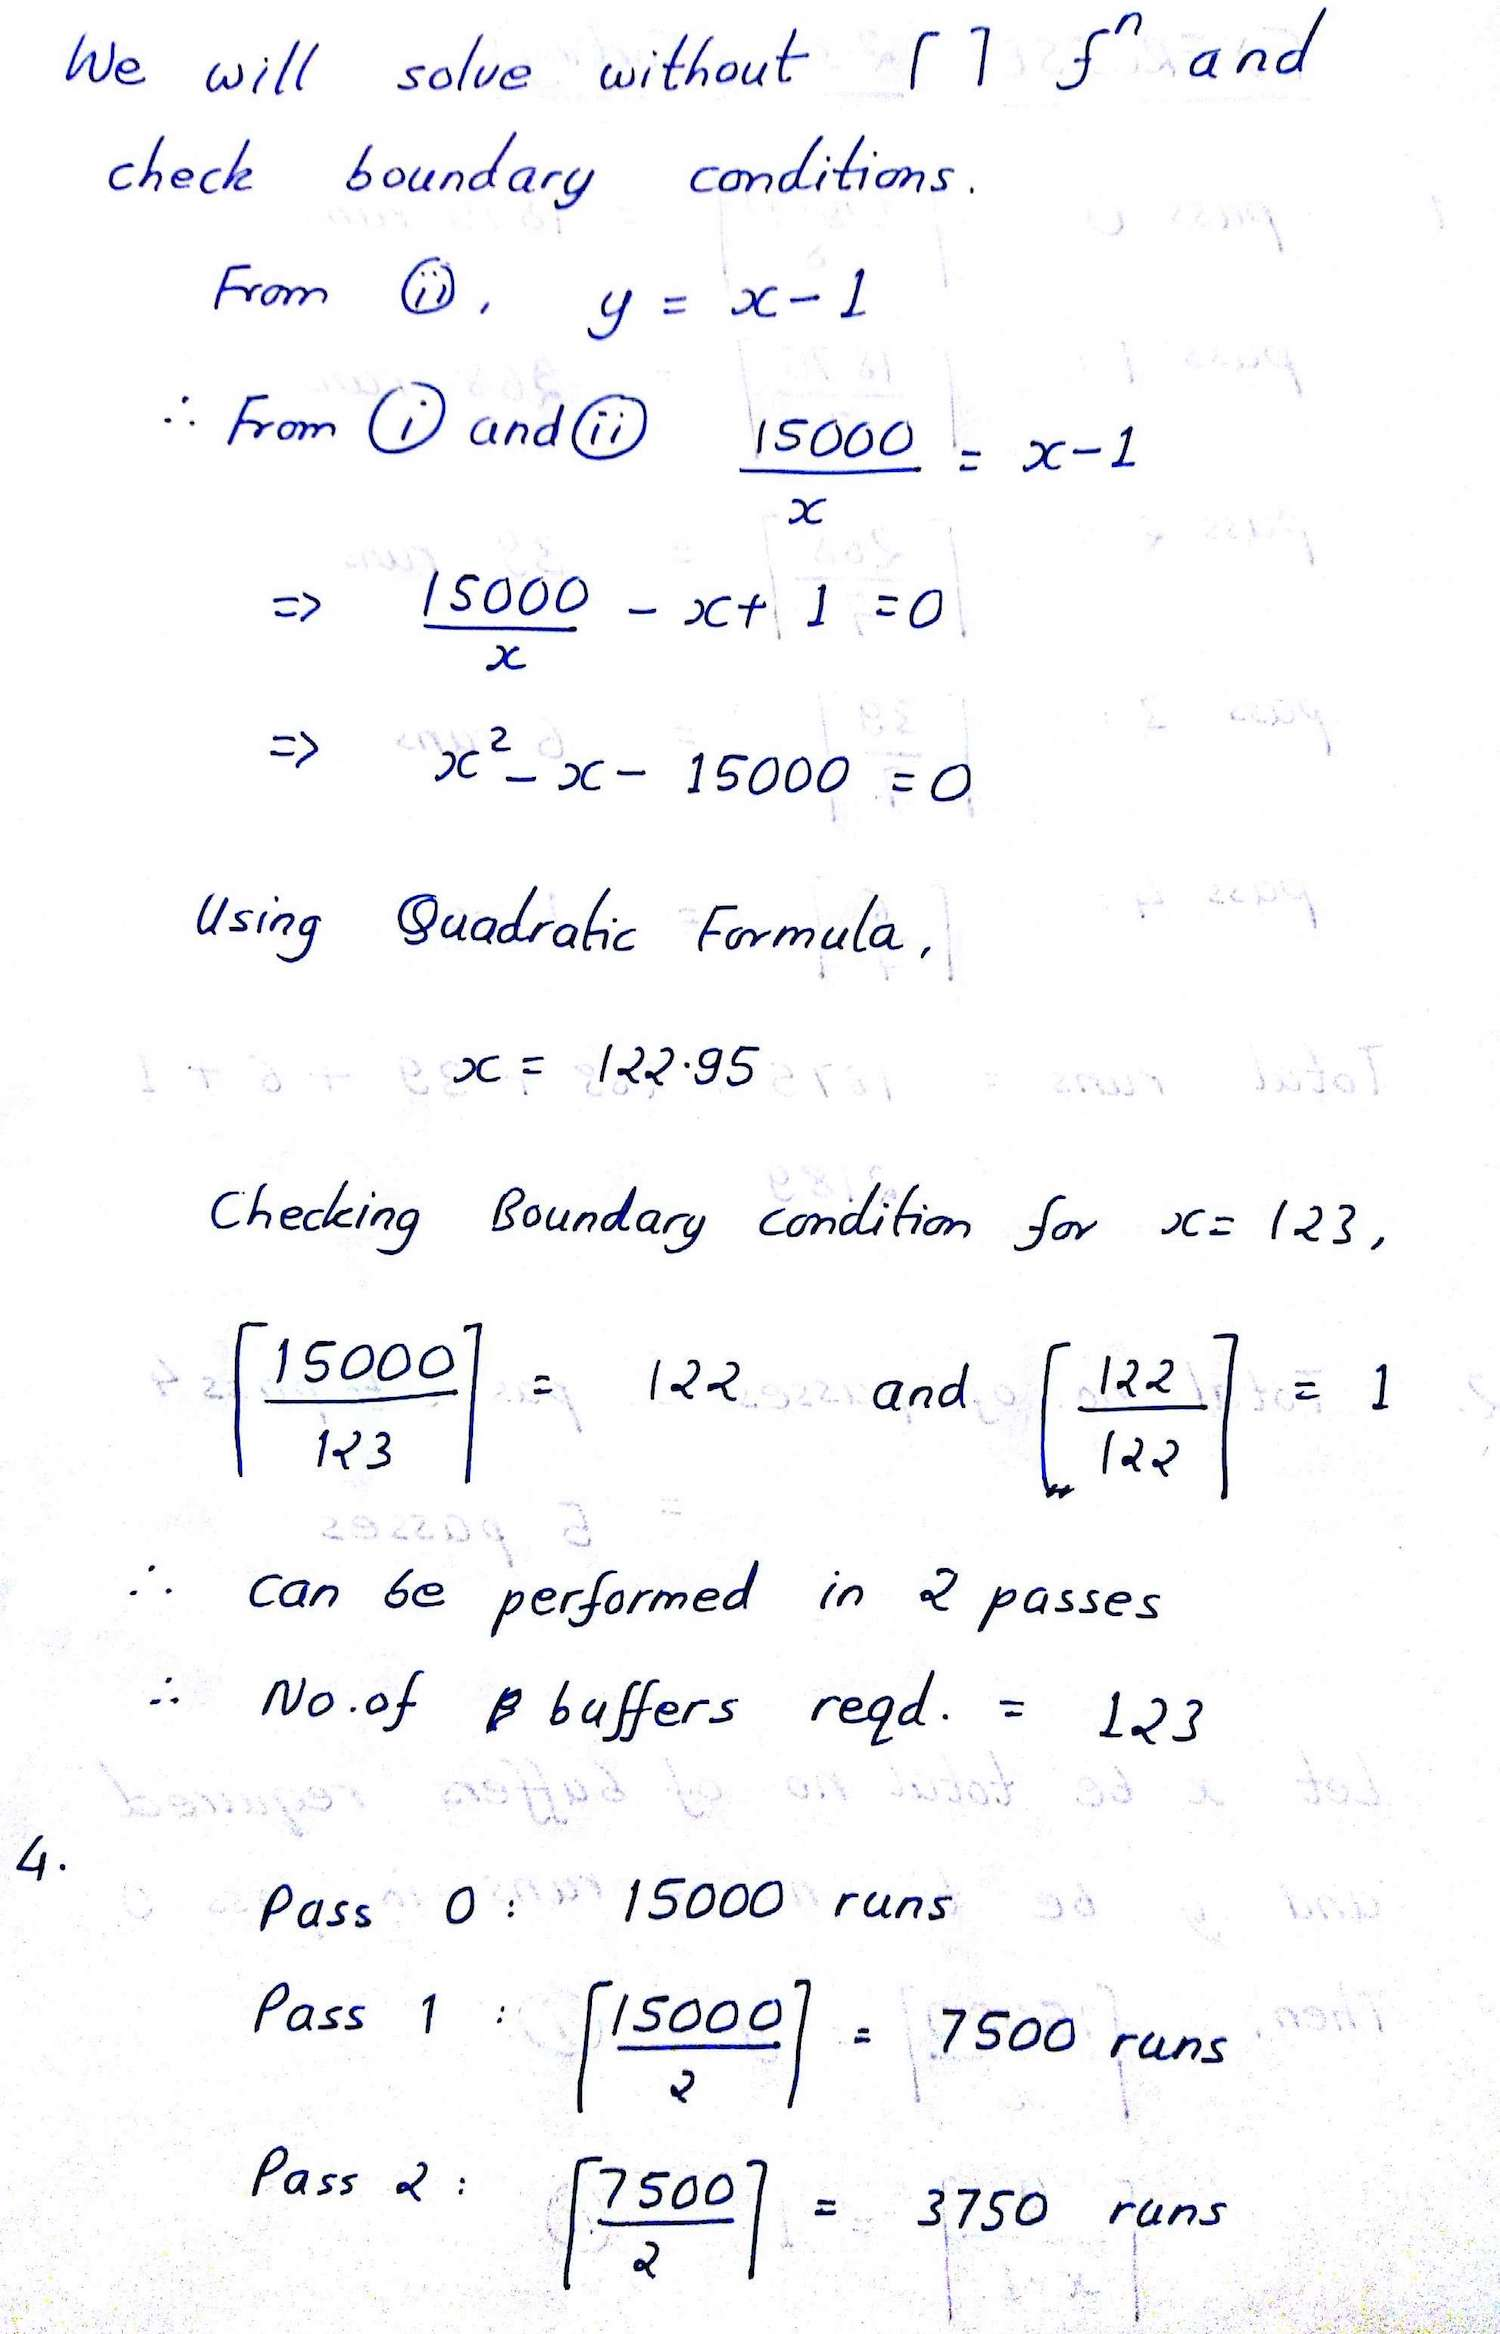
\includegraphics[width=12cm]{images/sol32.jpg}
\caption{Paper-based Solution for Question 3-2}
\end{figure} 

\begin{figure}[h]
\centering
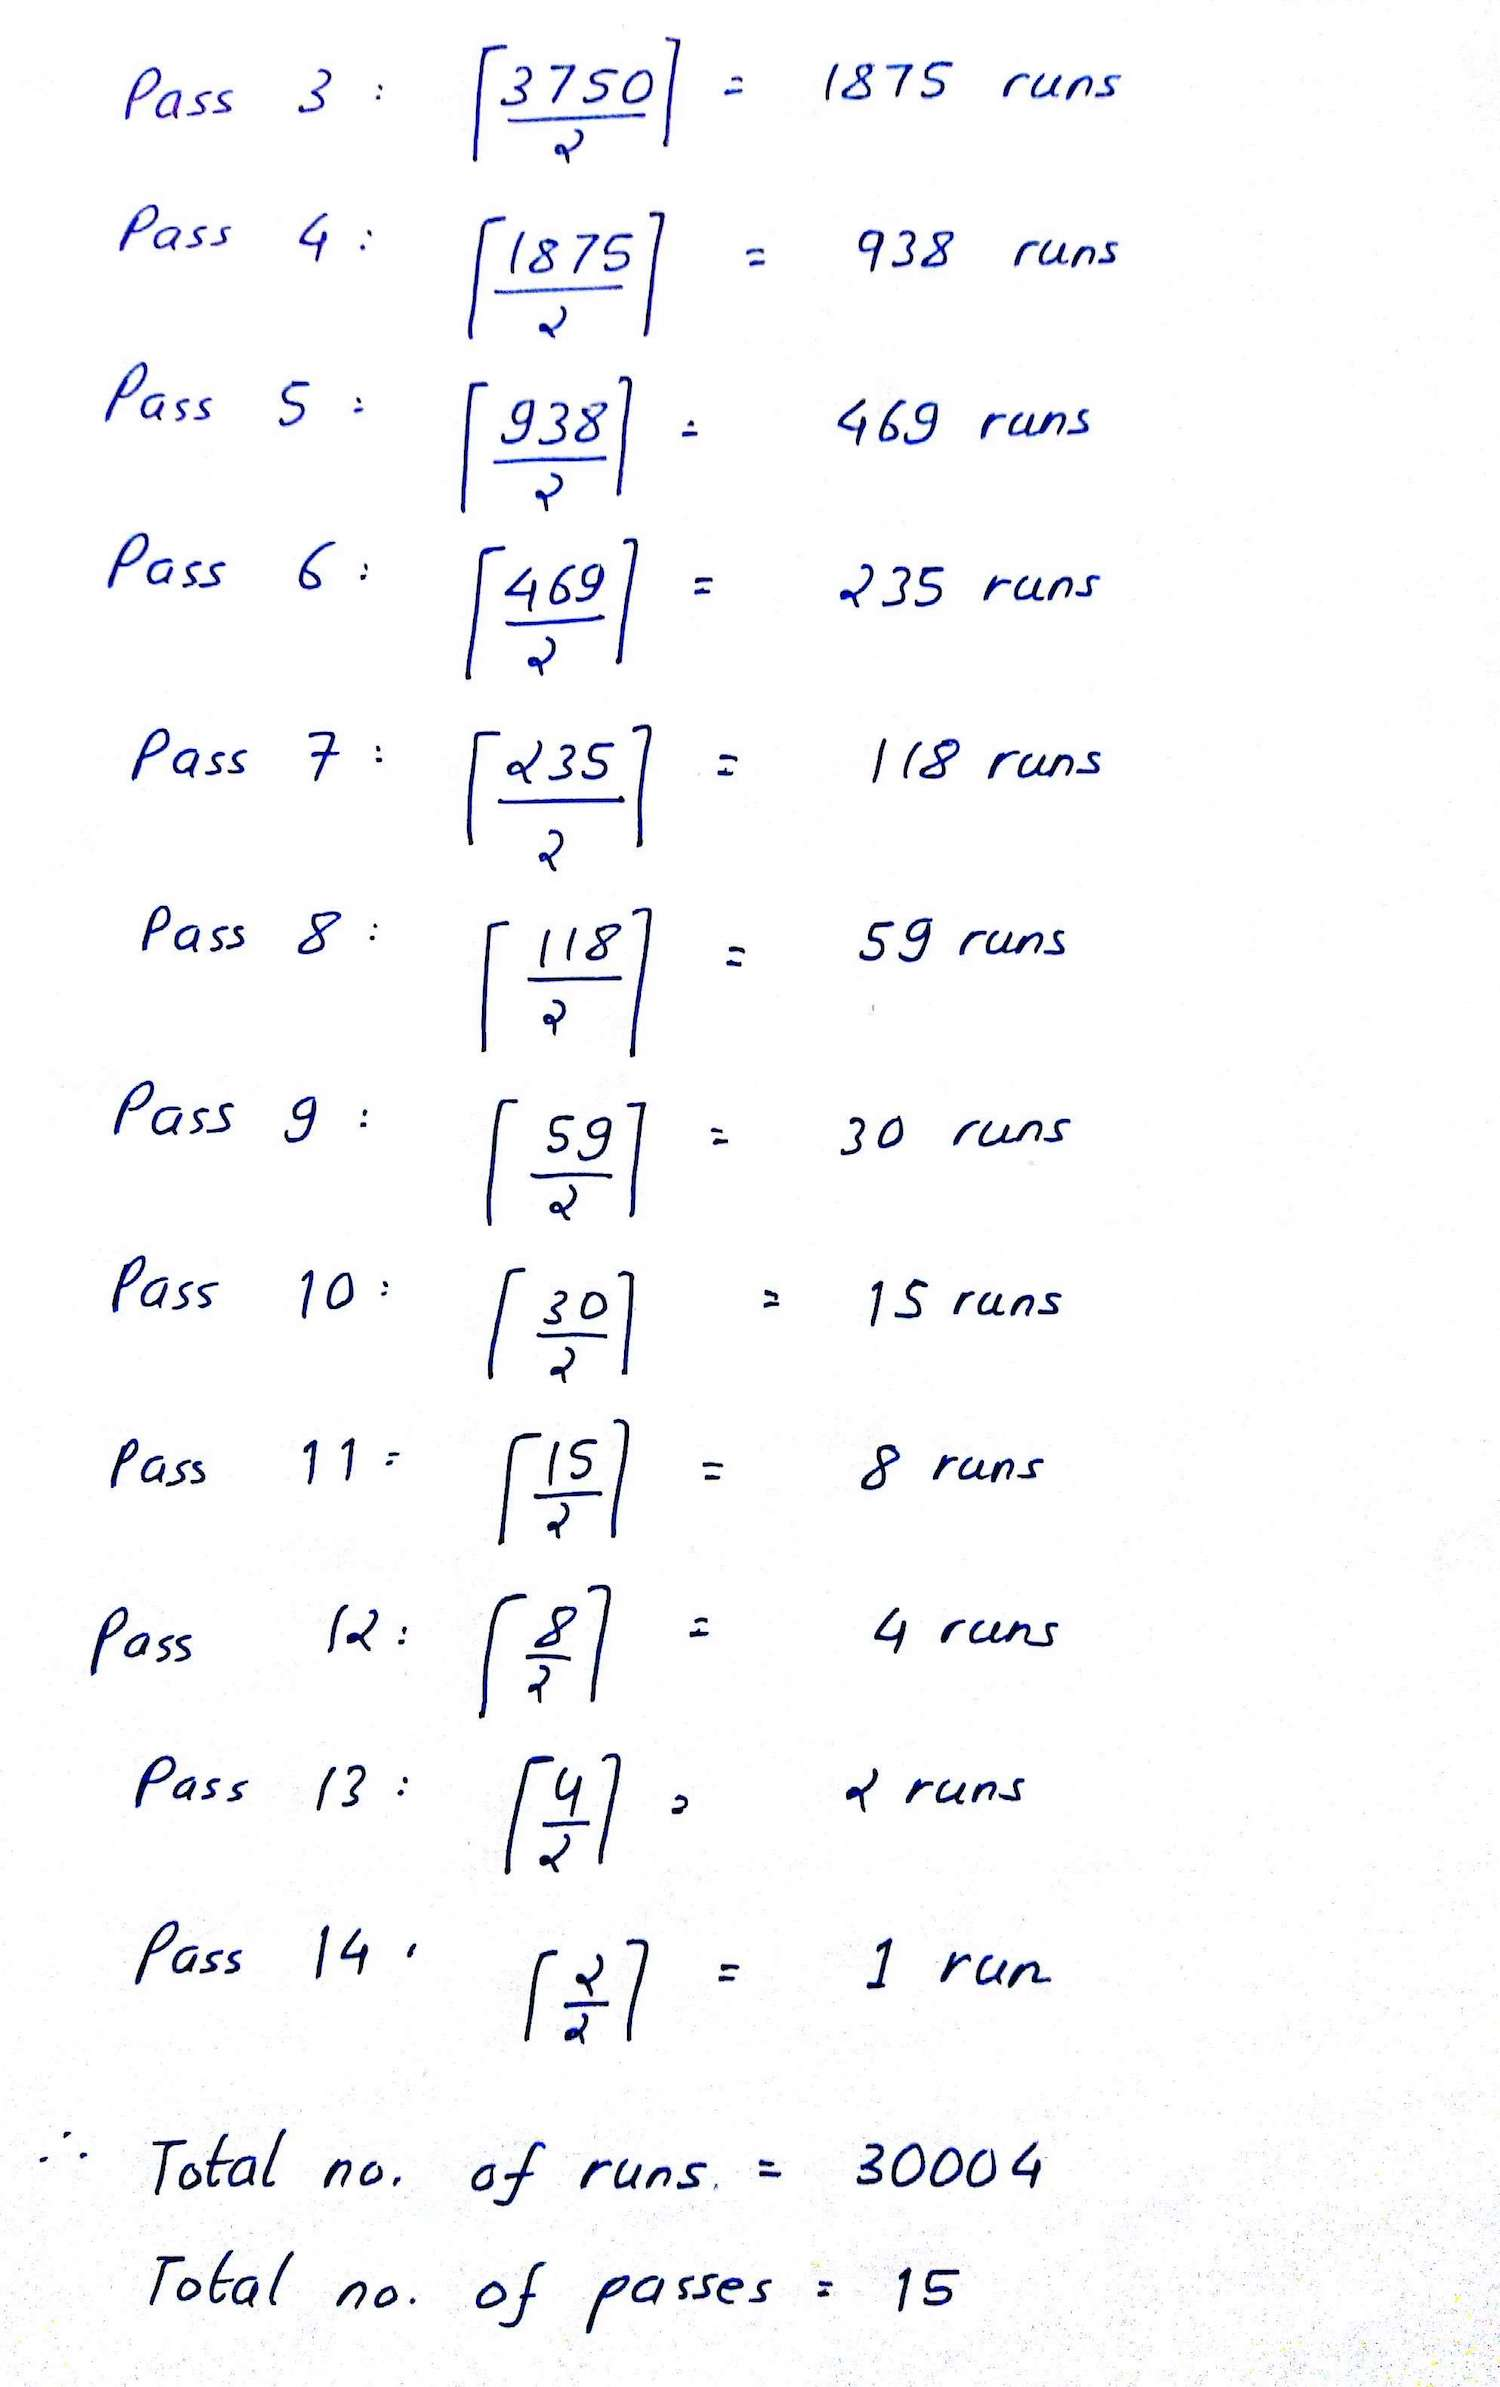
\includegraphics[width=12cm]{images/sol33.jpg}
\caption{Paper-based Solution for Question 3-3}
\end{figure} 

\end{homeworkProblem}

\begin{homeworkProblem}

\textbf{Part 1} \\
Calculate the I/O requirements of a simple nested loop join
 
 \vspace{0.1in} 
     \solution \\ \\ 
     %SOLUTION 
     In the expression below, M and N are the number of pages in the relations Album and Track respectively, $p_M$ and $p_N$ are the number of tuples in each page of the relations. \\
     
     \textbf{M as outer and N as inner relation} \\
     \textbf{Tuple-by-Tuple Simple Nested Loop Join} \\
     $M +  p_M \times M \times N$ \\
     $= 10000 + 100 \times 10000 \times 200000$ \\
     $ = 200000010000 $
          
    \vspace{0.1in}
     \textbf{Page-by-Page Simple Nested Loop Join} \\
     $M + M \times N$ \\
     $= 10000 + 10000 \times 200000$ \\
     $ = 2000010000 $
     
      \vspace{0.1in}
     \textbf{N as outer and M as inner relation} \\
     \textbf{Tuple-by-Tuple Simple Nested Loop Join} \\
     $N +  p_N \times N \times M$ \\
     $= 200000 + 80 \times 200000 \times 10000$ \\
     $ = 160000200000 $
          
    \vspace{0.1in}
     \textbf{Page-by-Page Simple Nested Loop Join} \\
     $M + M \times N$ \\
     $= 200000 + 200000 \times 10000$ \\
     $ = 2000200000 $
     \vspace{0.1in}
     
 \textbf{Part 2} \\
Calculate the I/O requirements of a block nested loop join
 
\vspace{0.1in} 
     \solution \\ \\ 
     %SOLUTION
     Block nested join for 16 buffers: \\
     
      \textbf{M as outer and N as inner relation} \\
     $ 10000 + \lceil \frac{10000}{14} \rceil \times 200000$
     $ = 143010000 $   
     \vspace{0.1in}
     
      \textbf{N as outer and M as inner relation} \\
      $ 200000 + \lceil \frac{200000}{14} \rceil \times 10000$
     $ = 143060000 $   
     \vspace{0.1in}
     
 \textbf{Part 3} \\
Explain the differences between the two algorithms. What are the similarities and differences? How does the block nested loop join reduce I/O costs?
 
 \vspace{0.1in} 
     \solution \\ \\ 
     %SOLUTION
     Tuple-at-a-time Simple Nested Loop Join scans outer relation and then for each tuple, it scans the entire inner relation. On the other hand, the page-at-a-time Simple Nested Loop Join will load the outer relation page-by-page, and then the inner relation for each page. The Block Nested Loop Join, on the other hand, scans entire inner relation for each block of pages in the outer relation. Therefore, the I/O cost of Block Nested Loop Join is lower than cost of both the Simple Nested Loop Joins. 
Moreover, the other important difference is number of buffer pages used in the algorithms. Both tuple-at-a-time nested loop and page-at-time nested loop join use 3 buffer pages to perform the join operation. 1 page as input buffer to scan outer relation,1 page as input buffer to scan inner relation  and 1 page as output buffer. Totally, 3 pages are needed for simple nested loop join. However, block nested loop join uses 1 page as input buffer to scan inner relation S and 1 page as output buffer. The other remaining buffer pages are used to load the blocks of the outer relation R. In this case, 1 buffer page is used as input buffer to scan inner relation  and 1 page as output buffer. Remaining 14 buffer pages are used to block outer relation . As seen, block nested loop join uses entire available buffer pages in the algorithm that means more efficient usage of buffer pages and causing performance increases and decreasing I/O cost. 

The similarities can be indicated as outer-inner relation usage, buffer usage and loop operations in the algorithms. 

     \vspace{0.1in}
     
\end{homeworkProblem}
     
\begin{homeworkProblem}
Given is a relation with 50.000 records. Each page for a node in a B+ tree can hold 20 pointers
to records or pages. A data page can store 20 records. \\

 \textbf{Part 1} \\
Assume that each node is 70 \% full. What is the height of the B+-tree? 

 \vspace{0.1in} 
     \solution \\ \\ 
     %SOLUTION  
     Given that the B+Tree can hold 20 pointers to pages. However, the B+ Tree has 70\% occupancy. Therefore, number of effective pointers to pages that the tree can hold,
     \begin{center} $ \implies 0.7 \times 20 = 14$ \end{center} 
Our B+ Tree can now be represented as Table 1

\begin{table}[]
\centering
\begin{tabular}{|l|l|l|l|}
\hline
Level    & Node & Entries & No. of Pointers \\ \hline
0 (Root) & 1    & 13      & 14              \\ \hline
1        & 14   & 182     & 196             \\ \hline
2        & 196  & 2548    & 2744         \\ \hline  
\end{tabular}
\caption{Different Levels of the B+ Tree}
\label{B+ Tree}
\end{table}

We have 2744 addresses in Level 2 already, which is more than 2500 pointers to pages required in the relations. \\
Therefore, the B-Tree has a depth of \textbf{3}.
Our B+ Tree has a depth of \textbf{3}
 \vspace{0.1in}
     
 \textbf{Part 2} \\
What are the I/O costs for an equality selection on a non-key attribute for the following
cases?

\begin{enumerate}[label = (\alph*)]
\item with a clustered B+-tree of height 3 (matching records are located in one page);
 
 \vspace{0.1in} 
     \solution \\ \\ 
     %SOLUTION
     The clustered index will guide the search, and after the end of the B+ tree traversal, we will need to input the correct page which contains our desired result. Therefore, total I/O is for the tree traversal and retrieving the correct page, i.e. 3 I/Os + 1 I/O = 4.
     Hence, total number of I/Os = \textbf{4} I/Os
     \vspace{0.1in}
     
\item without any index, nor is the file sorted on the attribute occurring in selection;

\vspace{0.1in} 
     \solution \\ \\ 
     %SOLUTION 
     Total number of pages at the leaf node = 2500
    If we consider that all pages need to be scanned, then the I/O costs will be \textbf{2500} I/Os. \\
    However, assuming, on an average that half the total number of pages need to be searched to find the equality results, it gives a total of 1250 I/Os.
          
     \vspace{0.1in}
     
\item with an unclustered B+-tree index of height 4, and there are 2 matching records;

\vspace{0.1in} 
     \solution \\ \\ 
     4 I/Os to traverse the tree + 2 I/Os to retrieve the matching records = \textbf{6} I/Os 
     \vspace{0.1in}

\item with an unclustered B+-tree of height 5 and three tenth of the records match the
selection.

\vspace{0.1in} 
\solution \\ \\ 
     %SOLUTION
     No. of matching records = $\frac{3}{10} \times 50000 = 15000$ records \\
     In the worst case, we need to do 15000 page I/Os, one for each record. Plus the I/Os for traversing the tree. Therefore, a total of 15000 I/Os + 5 I/Os = \textbf{15005} I/Os.   
     \vspace{0.1in}

\end{enumerate}
\end{homeworkProblem}

\end{document}
l\documentclass[12pt]{article}

\usepackage{fancyhdr}
\usepackage{extramarks}
\usepackage{amsmath}
\usepackage{amsthm}
\usepackage{amsfonts}
\usepackage{tikz}
\usepackage[plain]{algorithm}
\usepackage{algpseudocode}
\usepackage[export]{adjustbox}
\usepackage[latin1]{inputenc}           %For German characters
\usepackage{enumitem}               %For changing enumeration character
\usepackage{listings}               %For code
\usepackage{csquotes}
\usepackage{graphicx}               %For graphics e.g, images

\usetikzlibrary{automata,positioning}

%
% Basic Document Settings
%

\topmargin=-0.45in
\evensidemargin=0in
\oddsidemargin=0in
\textwidth=6.5in
\textheight=9.0in
\headsep=0.25in

\linespread{1.1}

\pagestyle{fancy}
\lhead{\hmwkAuthorName}
\chead{\hmwkClass\ : \hmwkTitle}
\rhead{\firstxmark}
\lfoot{\lastxmark}
\cfoot{\thepage}

\renewcommand\headrulewidth{0.4pt}
\renewcommand\footrulewidth{0.4pt}

\setlength\parindent{0pt}

%
% Create Problem Sections
%

\newcommand{\enterProblemHeader}[1]{
    \nobreak\extramarks{}{Problem \arabic{#1} continued on next page\ldots}\nobreak{}
    \nobreak\extramarks{Problem \arabic{#1} (continued)}{Problem \arabic{#1} continued on next page\ldots}\nobreak{}
}

\newcommand{\exitProblemHeader}[1]{
    \nobreak\extramarks{Problem \arabic{#1} (continued)}{Problem \arabic{#1} continued on next page\ldots}\nobreak{}
    \stepcounter{#1}
    \nobreak\extramarks{Problem \arabic{#1}}{}\nobreak{}
}

\setcounter{secnumdepth}{0}
\newcounter{partCounter}
\newcounter{homeworkProblemCounter}
\setcounter{homeworkProblemCounter}{1}
\nobreak\extramarks{Problem \arabic{homeworkProblemCounter}}{}\nobreak{}

%
% Homework Problem Environment
%
% This environment takes an optional argument. When given, it will adjust the
% problem counter. This is useful for when the problems given for your
% assignment aren't sequential. See the last 3 problems of this template for an
% example.
%
\newenvironment{homeworkProblem}[1][-1]{
    \ifnum#1>0
        \setcounter{homeworkProblemCounter}{#1}
    \fi
    \section{Problem \arabic{homeworkProblemCounter}}
    \setcounter{partCounter}{1}
    \enterProblemHeader{homeworkProblemCounter}
}{
    \exitProblemHeader{homeworkProblemCounter}
}

%
% Homework Details
%   - Title
%   - Due date
%   - Class
%   - Section/Time
%   - Instructor
%   - Author
%

\newcommand{\hmwkTitle}{Assignment\ \#2}
\newcommand{\hmwkDueDate}{November 15, 2016}
\newcommand{\hmwkClass}{Implementation of Databases}
\newcommand{\hmwkAuthorName}{Sanchit Alekh}
\newcommand{\hmwkClassTime}{MSc. Software Systems Engineering}
\newcommand{\hmwkClassInstructor}{Universitätsprofessor Dr. rer. pol. Matthias Jarke}
\newcommand{\hmwkClassInstructors}{Dr. rer. nat. Christoph Quix}

%
% Title Page
%



\title{
   \begin{center}
   \vspace*{-20mm}
   \includegraphics[width=0.4\textwidth, right]{images/rwth_logo.png}
   \\
   \vspace*{3cm}
    \textmd{\textbf{\hmwkClass}}\\
    \textmd{\textbf{\hmwkTitle}}\\
    \normalsize\vspace{0.1in}\small{Due\ on\ \hmwkDueDate } \\
    \vspace{0.1in}\large{\textit{\hmwkClassInstructor}} \\
    \vspace{0.1in}\large{\textit{\hmwkClassInstructors}} \\
    \vspace{3in}
     \textbf{Submitted by:} \\
     \vspace{0.25in}
    \large{Sanchit Alekh, Idil Esen Zülfikar, Nihal Hegde} \\
    %\author{\textbf{\hmwkAuthorName}}
    \vspace{0.1in} \large{\textit{\hmwkClassTime}} \\
    %\vspace{0.1in} \large{\textit{Matrikelnummer : 359831}}
    \end{center}
    }


\date{}

\renewcommand{\part}[1]{\textbf{\large Part \Alph{partCounter}}\stepcounter{partCounter}\\}

%
% Various Helper Commands
%

% Useful for algorithms
\newcommand{\alg}[1]{\textsc{\bfseries \footnotesize #1}}

% For derivatives
\newcommand{\deriv}[1]{\frac{\mathrm{d}}{\mathrm{d}x} (#1)}

% For partial derivatives
\newcommand{\pderiv}[2]{\frac{\partial}{\partial #1} (#2)}

% Integral dx
\newcommand{\dx}{\mathrm{d}x}

% Alias for the Solution section header
\newcommand{\solution}{\textbf{\large Solution}}

% Probability commands: Expectation, Variance, Covariance, Bias
\newcommand{\E}{\mathrm{E}}
\newcommand{\Var}{\mathrm{Var}}
\newcommand{\Cov}{\mathrm{Cov}}
\newcommand{\Bias}{\mathrm{Bias}}

\begin{document}

\maketitle

\pagebreak

\begin{homeworkProblem}
    
    \textbf{Part 1} \\
    Variants of relational algebra are used internally in DBMS to represent queries and query evaluation plans. Please explain, why relational algebra is suitable for this?
    
    \vspace{0.1in}
    \solution \\
    One of the most desirable properties of Relational Algebra is that queries are composed using a collection of operators, and every operator accepts one or two relation instances as arguments and returns a relation instance as the result. This property makes extremely easy and efficient to compose operators to form a complex query. A relational algebra expression can be recursively defined to be a relation, a unary algebra operator applied to a single expression, or a binary algebra operator applied to two expressions. 
This procedural nature of relational algebra is the main reason why it is used internally in DBMS to represent queries and evaluation plans. The approach allows us to think of an algebra expression as an imperative execution plan for a declarative SQL query. It can be used for evaluating a query, and relational systems in fact use algebra expressions to represent query evaluation plans.
        
    \vspace{0.1in}
    
    \textbf{Part 2} \\
    What does \enquote{relational completeness} mean (in your own words, please)? Show that SQL is
relationally complete by enumerating SQL constructs corresponding to selection, projection,
cartesian product, union, and difference.
    
    \vspace{0.1in}
    \solution \\
    \enquote{Relational Completeness} of a query methodology means that each and every query that can be expressed using that methodology, can also be expressed as a relational algebra query. In this case, SQL is referred to as \enquote*{Relationally Complete} because every legal construct in SQL can be expressed as a Relational Algebra query.
        
These are the examples of Relational Algebra expressions and their equivalent expressions in SQL. The following examples are derived from the \textit{Mondial} database.

\begin{itemize}

\item \textbf{SELECTION} \\
Relational Algebra: $ \sigma_{Area > 650} (Island)$ \\
SQL:  \textit{Select * From Island Where Area $>$ 650;}

\item \textbf{PROJECTION} \\
Relational Algebra: $ \pi_{Name, Islands, Area, Height} (Island)$ \\
SQL: \textit{Select Name, Islands, Area, Height From Island;}

\item \textbf{CARTESIAN PRODUCT} \\
Relational Algebra:  $ Island \times islandIn$ \\
SQL: \textit{Select * From Island CROSS JOIN islandIn;}

\item \textbf{UNION} \\
Relational Algebra:  $ \pi_{name} (Desert) \cup \pi_{name} (geo\_Desert)$ \\
SQL: \textit{Select name From Desert or Select name From geo\_Desert}

\item \textbf{SET DIFFERENCE} \\
Relational Algebra: $ \pi_{name} (\sigma_{height > 5000} (Mountain)) - \pi_{name}( \sigma_{type > 'volcanic')} (Mountain) $ \\
SQL: \textit{Select name From Mountain where height $>$ 5000 MINUS Select name From Mountain where type='volcanic'}
\end{itemize}
        
    \vspace{0.1in}
        
     \textbf{Part 3} \\
    Explain how the intersection operator is used in relational algebra. What is important for
its usage? Is it omittable (i.e., could you express it by other operators)? If so, please give
the corresponding relational algebra.
    
    \vspace{0.1in}
    \solution \\
    The \enquote*{Intersection} operator is represented in Relational Algebra with the help of the $\cap$ symbol. Although it is not a fundamental set-operator, it is an extremely widely used operation, and it is helpful to define it separately. An example use of the intersection operator is as follows:
    
    \begin{center} $ \pi_{name} (Desert) \cap \pi_{name} (geo\_Desert) $ \end{center}
    
The important condition for using the \textit{Intersection} operator is that the two sets which have to be intersected must be \textit{union-compatible}. This follows from the fact that intersection is defined in terms of set difference.

Yes, Intersection is not a fundamental set-operator, and it can be expressed in terms of the set-difference operator. Therefore, it is omittable. A general expression for the intersection operator in terms of the set-difference operator is:

    \begin{center} $ A \cup B \leftrightarrow A \setminus ( A \setminus B) $ \end{center}
    
Therefore, the example Relational Algebra query illustrated above can be represented by the equivalent query without the use of set-intersection as follows:

    \begin{center} $ \pi_{name} (Desert) - (\pi_{name} (Desert) - \pi_{name} (geo\_Desert))$ \end{center}
    
\begin{figure}[h]
\centering
\includegraphics[width=12cm]{images/intersection1.png}
\caption{Venn-Diagram showing the definition of Intersection in terms of Set Difference}
\end{figure}
        
    \vspace{0.1in}
    
     \textbf{Part 4} \\
    Explain the difference between DRC and TRC.
    
    \vspace{0.1in}
        \solution \\
In Tuple Relational Calculus (TRC), the variables typically range over tuples, i.e. they directly represent tuples. On the other hand, in Domain Relational Calculus (DRC), the variables range over domain elements, i.e. field values. In TRC, tuples are semantically equivalent to variables, i.e. field referencing can be used to select tuple parts. On the other hand, in DRC, formal variables are explicit and have to be defined.
    \vspace{0.1in}
    
    
\end{homeworkProblem}   

\begin{homeworkProblem}

\textbf{Part 1} \\

The names of the seas that are deeper than 3000 mt and into which at least one river finally flows.

\vspace{0.1in}
    \solution \\
      
    $<name> \mid \exists depth, rname, river, lake, sea, length, sLong, sLat, mount, sAlt, estLong, estLat \\
    Sea(name, depth) \wedge  \\ River(rname, river, lake, sea, length, sLong, sLat, mount, sAlt, estLong, estLat) \wedge \\ depth > 3000 \wedge sea = name$ 
    \vspace{0.1in}
    
\textbf{Part 2} \\
The names of the groups of islands that consist only of islands that are neither 'volcanic' nor
'coral'.

 \vspace{0.1in}
    \solution \\ \\    
   %SOLUTION
   $<islands> \mid \exists name, area, height, type, long, lat \\
Island(name, islands, area, height, type, long, lat) \wedge \\
type \notin \{volcanic, coral\} \wedge islands \neq \emptyset  $
    \vspace{0.1in}    

\textbf{Part 3} \\
The name of the mountain, the name of the mountains where it belongs to and the name of
the country where the mountain is located for each mountain that is located on an island
that is of type 'coral'.

 
 \vspace{0.1in} 
     \solution \\ \\ 
     %SOLUTION   
     $<moiMountain, mMountains, gmCountry> \mid \exists \\ moiIsland, mHeight, mType, mLong, mLat, \\ iIslands, iArea, iHeight, iType, iLong, iLat, gmProvince \\
mountainOnIsland(moiMountain, moiIsland) \wedge \\ Mountain(moiMountain, mMountains, mHeight, mType, mLong, mLat) \wedge \\ geo\_Mountain(moiMountain, gmCountry, gmProvince)  \wedge \\
Island(moiIsland, iIslands, iArea, iHeight, iType, iLong, iLat) \wedge iType \neq "coral" $

     \vspace{0.1in}

    
\textbf{Part 4} \\
Give the name and country name of all cities with a population higher than 500,000.

 \vspace{0.1in} 
     \solution \\ \\    
    %SOLUTION
   $<cName, coName> \mid \exists cCountry, cProvince, cPopulation, cLong, cLat, \\
   coCapital, coProvince, coArea, coPopulation \\
City(cName, cCountry, cProvince, cPopulation, cLong, cLat)  \wedge \\
Country(cCountry, coName, coCapital, coProvince, coArea, coPopulation) \wedge \\
cPopulation > 500000 $
 
    \vspace{0.1in}
        
\end{homeworkProblem}

\begin{homeworkProblem}
Suppose you have a file of 15,000 pages and eight buffer pages and you are sorting it using general
(external) merge-sort. Please answer the following questions: \\

\textbf{Part 1} \\
How many runs will you produce? Remark: When a file is sorted, in intermediate steps
subfiles are created. Each sorted subfile is called a run. See also slide 35 in Chapter 2.
 \textbf{Note: Detailed solution of Q3 is produced in \textit{Figures 2, 3 and 4.}}
 
 \vspace{0.1in} 
     \solution \\
     %SOLUTION
     \textbf{2189} runs will be produced   
     \vspace{0.1in}
     
 \textbf{Part 2} \\
How many passes will it take to sort the file completely?
 
 \vspace{0.1in} 
     \solution \\ 
    It will take \textbf{5} passes   
     \vspace{0.1in}
     
 \textbf{Part 3} \\
How many buffer pages do you need at least to sort the file in two passes? 

 \vspace{0.1in} 
     \solution \\
     With \textbf{123} buffers, you can sort the file in two passes 
     \vspace{0.1in}
 
 \textbf{Part 4} \\
How many runs and passes would a Two-Way-Sort algorithm take?
 
 \vspace{0.1in} 
     \solution \\
     %SOLUTION
     Two-Way Sort Algorithm will take \textbf{30004} runs and \textbf{15} passes   
     \vspace{0.1in}   
     
\begin{figure}[h]
\centering
\includegraphics[width=12cm]{images/sol31.jpg}
\caption{Paper-based Solution for Question 3-1}
\end{figure} 

\begin{figure}[h]
\centering
\includegraphics[width=12cm]{images/sol32.jpg}
\caption{Paper-based Solution for Question 3-2}
\end{figure} 

\begin{figure}[h]
\centering
\includegraphics[width=12cm]{images/sol33.jpg}
\caption{Paper-based Solution for Question 3-3}
\end{figure} 

\end{homeworkProblem}

\begin{homeworkProblem}

\textbf{Part 1} \\
Calculate the I/O requirements of a simple nested loop join
 
 \vspace{0.1in} 
     \solution \\ \\ 
     %SOLUTION 
     In the expression below, M and N are the number of pages in the relations Album and Track respectively, $p_M$ and $p_N$ are the number of tuples in each page of the relations. \\
     
     \textbf{M as outer and N as inner relation} \\
     \textbf{Tuple-by-Tuple Simple Nested Loop Join} \\
     $M +  p_M \times M \times N$ \\
     $= 10000 + 100 \times 10000 \times 200000$ \\
     $ = 200000010000 $
          
    \vspace{0.1in}
     \textbf{Page-by-Page Simple Nested Loop Join} \\
     $M + M \times N$ \\
     $= 10000 + 10000 \times 200000$ \\
     $ = 2000010000 $
     
      \vspace{0.1in}
     \textbf{N as outer and M as inner relation} \\
     \textbf{Tuple-by-Tuple Simple Nested Loop Join} \\
     $N +  p_N \times N \times M$ \\
     $= 200000 + 80 \times 200000 \times 10000$ \\
     $ = 160000200000 $
          
    \vspace{0.1in}
     \textbf{Page-by-Page Simple Nested Loop Join} \\
     $M + M \times N$ \\
     $= 200000 + 200000 \times 10000$ \\
     $ = 2000200000 $
     \vspace{0.1in}
     
 \textbf{Part 2} \\
Calculate the I/O requirements of a block nested loop join
 
\vspace{0.1in} 
     \solution \\ \\ 
     %SOLUTION
     Block nested join for 16 buffers: \\
     
      \textbf{M as outer and N as inner relation} \\
     $ 10000 + \lceil \frac{10000}{14} \rceil \times 200000$
     $ = 143010000 $   
     \vspace{0.1in}
     
      \textbf{N as outer and M as inner relation} \\
      $ 200000 + \lceil \frac{200000}{14} \rceil \times 10000$
     $ = 143060000 $   
     \vspace{0.1in}
     
 \textbf{Part 3} \\
Explain the differences between the two algorithms. What are the similarities and differences? How does the block nested loop join reduce I/O costs?
 
 \vspace{0.1in} 
     \solution \\ \\ 
     %SOLUTION
     Tuple-at-a-time Simple Nested Loop Join scans outer relation and then for each tuple, it scans the entire inner relation. On the other hand, the page-at-a-time Simple Nested Loop Join will load the outer relation page-by-page, and then the inner relation for each page. The Block Nested Loop Join, on the other hand, scans entire inner relation for each block of pages in the outer relation. Therefore, the I/O cost of Block Nested Loop Join is lower than cost of both the Simple Nested Loop Joins. 
Moreover, the other important difference is number of buffer pages used in the algorithms. Both tuple-at-a-time nested loop and page-at-time nested loop join use 3 buffer pages to perform the join operation. 1 page as input buffer to scan outer relation,1 page as input buffer to scan inner relation  and 1 page as output buffer. Totally, 3 pages are needed for simple nested loop join. However, block nested loop join uses 1 page as input buffer to scan inner relation S and 1 page as output buffer. The other remaining buffer pages are used to load the blocks of the outer relation R. In this case, 1 buffer page is used as input buffer to scan inner relation  and 1 page as output buffer. Remaining 14 buffer pages are used to block outer relation . As seen, block nested loop join uses entire available buffer pages in the algorithm that means more efficient usage of buffer pages and causing performance increases and decreasing I/O cost. 

The similarities can be indicated as outer-inner relation usage, buffer usage and loop operations in the algorithms. 

     \vspace{0.1in}
     
\end{homeworkProblem}
     
\begin{homeworkProblem}
Given is a relation with 50.000 records. Each page for a node in a B+ tree can hold 20 pointers
to records or pages. A data page can store 20 records. \\

 \textbf{Part 1} \\
Assume that each node is 70 \% full. What is the height of the B+-tree? 

 \vspace{0.1in} 
     \solution \\ \\ 
     %SOLUTION  
     Given that the B+Tree can hold 20 pointers to pages. However, the B+ Tree has 70\% occupancy. Therefore, number of effective pointers to pages that the tree can hold,
     \begin{center} $ \implies 0.7 \times 20 = 14$ \end{center} 
Our B+ Tree can now be represented as Table 1

\begin{table}[]
\centering
\begin{tabular}{|l|l|l|l|}
\hline
Level    & Node & Entries & No. of Pointers \\ \hline
0 (Root) & 1    & 13      & 14              \\ \hline
1        & 14   & 182     & 196             \\ \hline
2        & 196  & 2548    & 2744         \\ \hline  
\end{tabular}
\caption{Different Levels of the B+ Tree}
\label{B+ Tree}
\end{table}

We have 2744 addresses in Level 2 already, which is more than 2500 pointers to pages required in the relations. \\
Therefore, the B-Tree has a depth of \textbf{3}.
Our B+ Tree has a depth of \textbf{3}
 \vspace{0.1in}
     
 \textbf{Part 2} \\
What are the I/O costs for an equality selection on a non-key attribute for the following
cases?

\begin{enumerate}[label = (\alph*)]
\item with a clustered B+-tree of height 3 (matching records are located in one page);
 
 \vspace{0.1in} 
     \solution \\ \\ 
     %SOLUTION
     The clustered index will guide the search, and after the end of the B+ tree traversal, we will need to input the correct page which contains our desired result. Therefore, total I/O is for the tree traversal and retrieving the correct page, i.e. 3 I/Os + 1 I/O = 4.
     Hence, total number of I/Os = \textbf{4} I/Os
     \vspace{0.1in}
     
\item without any index, nor is the file sorted on the attribute occurring in selection;

\vspace{0.1in} 
     \solution \\ \\ 
     %SOLUTION 
     Total number of pages at the leaf node = 2500
    If we consider that all pages need to be scanned, then the I/O costs will be \textbf{2500} I/Os. \\
    However, assuming, on an average that half the total number of pages need to be searched to find the equality results, it gives a total of 1250 I/Os.
          
     \vspace{0.1in}
     
\item with an unclustered B+-tree index of height 4, and there are 2 matching records;

\vspace{0.1in} 
     \solution \\ \\ 
     4 I/Os to traverse the tree + 2 I/Os to retrieve the matching records = \textbf{6} I/Os 
     \vspace{0.1in}

\item with an unclustered B+-tree of height 5 and three tenth of the records match the
selection.

\vspace{0.1in} 
\solution \\ \\ 
     %SOLUTION
     No. of matching records = $\frac{3}{10} \times 50000 = 15000$ records \\
     In the worst case, we need to do 15000 page I/Os, one for each record. Plus the I/Os for traversing the tree. Therefore, a total of 15000 I/Os + 5 I/Os = \textbf{15005} I/Os.   
     \vspace{0.1in}

\end{enumerate}
\end{homeworkProblem}

\end{document}

\usetikzlibrary{automata,positioning}

%
% Basic Document Settings
%

\topmargin=-0.45in
\evensidemargin=0in
\oddsidemargin=0in
\textwidth=6.5in
\textheight=9.0in
\headsep=0.25in

\linespread{1.1}

\pagestyle{fancy}
\lhead{\hmwkAuthorName}
\chead{\hmwkClass\ : \hmwkTitle}
\rhead{\firstxmark}
\lfoot{\lastxmark}
\cfoot{\thepage}

\renewcommand\headrulewidth{0.4pt}
\renewcommand\footrulewidth{0.4pt}

\setlength\parindent{0pt}

%
% Create Problem Sections
%

\newcommand{\enterProblemHeader}[1]{
\nobreak\extramarks{}{Problem \arabic{#1} continued on next page\ldots}\nobreak{}
\nobreak\extramarks{Problem \arabic{#1} (continued)}{Problem \arabic{#1} continued on next page\ldots}\nobreak{}
}

\newcommand{\exitProblemHeader}[1]{
\nobreak\extramarks{Problem \arabic{#1} (continued)}{Problem \arabic{#1} continued on next page\ldots}\nobreak{}
\stepcounter{#1}
\nobreak\extramarks{Problem \arabic{#1}}{}\nobreak{}
}

\setcounter{secnumdepth}{0}
\newcounter{partCounter}
\newcounter{homeworkProblemCounter}
\setcounter{homeworkProblemCounter}{1}
\nobreak\extramarks{Problem \arabic{homeworkProblemCounter}}{}\nobreak{}

%
% Homework Problem Environment
%
% This environment takes an optional argument. When given, it will adjust the
% problem counter. This is useful for when the problems given for your
% assignment aren't sequential. See the last 3 problems of this template for an
% example.
%
\newenvironment{homeworkProblem}[1][-1]{
\ifnum#1>0
\setcounter{homeworkProblemCounter}{#1}
\fi
\section{Problem \arabic{homeworkProblemCounter}}
\setcounter{partCounter}{1}
\enterProblemHeader{homeworkProblemCounter}
}{
\exitProblemHeader{homeworkProblemCounter}
}

%
% Homework Details
%   - Title
%   - Due date
%   - Class
%   - Section/Time
%   - Instructor
%   - Author
%

\newcommand{\hmwkTitle}{Assignment\ \#2}
\newcommand{\hmwkDueDate}{November 15, 2016}
\newcommand{\hmwkClass}{Implementation of Databases}
\newcommand{\hmwkAuthorName}{Sanchit Alekh}
\newcommand{\hmwkClassTime}{MSc. Software Systems Engineering}
\newcommand{\hmwkClassInstructor}{Universitätsprofessor Dr. rer. pol. Matthias Jarke}
\newcommand{\hmwkClassInstructors}{Dr. rer. nat. Christoph Quix}

%
% Title Page
%
\title{
\begin{center}
\vspace*{-20mm}
\includegraphics[width=0.4\textwidth, right]{images/rwth_logo.png}
\\
\vspace*{3cm}
\textmd{\textbf{\hmwkClass}}\\
\textmd{\textbf{\hmwkTitle}}\\
\normalsize\vspace{0.1in}\small{Due\ on\ \hmwkDueDate } \\
\vspace{0.1in}\large{\textit{\hmwkClassInstructor}} \\
\vspace{0.1in}\large{\textit{\hmwkClassInstructors}} \\
\vspace{3in}
\textbf{Submitted by:} \\
\vspace{0.25in}
\large{Sanchit Alekh, Idil Esen Zülfikar, Nihal Hegde} \\
    %\author{\textbf{\hmwkAuthorName}}
    \vspace{0.1in} \large{\textit{\hmwkClassTime}} \\
    %\vspace{0.1in} \large{\textit{Matrikelnummer : 359831}}
    \end{center}
    }


    \date{}

    \renewcommand{\part}[1]{\textbf{\large Part \Alph{partCounter}}\stepcounter{partCounter}\\}

%
% Various Helper Commands
%

% Useful for algorithms
\newcommand{\alg}[1]{\textsc{\bfseries \footnotesize #1}}

% For derivatives
\newcommand{\deriv}[1]{\frac{\mathrm{d}}{\mathrm{d}x} (#1)}

% For partial derivatives
\newcommand{\pderiv}[2]{\frac{\partial}{\partial #1} (#2)}

% Integral dx
\newcommand{\dx}{\mathrm{d}x}

% Alias for the Solution section header
\newcommand{\solution}{\textbf{\large Solution}}

% Probability commands: Expectation, Variance, Covariance, Bias
\newcommand{\E}{\mathrm{E}}
\newcommand{\Var}{\mathrm{Var}}
\newcommand{\Cov}{\mathrm{Cov}}
\newcommand{\Bias}{\mathrm{Bias}}

\begin{document}

\maketitle

\pagebreak

\begin{homeworkProblem}

\textbf{Part 1} \\
Variants of relational algebra are used internally in DBMS to represent queries and query evaluation plans. Please explain, why relational algebra is suitable for this?

\vspace{0.1in}
\solution \\
One of the most desirable properties of Relational Algebra is that queries are composed using a collection of operators, and every operator accepts one or two relation instances as arguments and returns a relation instance as the result. This property makes extremely easy and efficient to compose operators to form a complex query. A relational algebra expression can be recursively defined to be a relation, a unary algebra operator applied to a single expression, or a binary algebra operator applied to two expressions. 
This procedural nature of relational algebra is the main reason why it is used internally in DBMS to represent queries and evaluation plans. The approach allows us to think of an algebra expression as an imperative execution plan for a declarative SQL query. It can be used for evaluating a query, and relational systems in fact use algebra expressions to represent query evaluation plans.

\vspace{0.1in}

\textbf{Part 2} \\
What does \enquote{relational completeness} mean (in your own words, please)? Show that SQL is
relationally complete by enumerating SQL constructs corresponding to selection, projection,
cartesian product, union, and difference.

\vspace{0.1in}
\solution \\
\enquote{Relational Completeness} of a query methodology means that each and every query that can be expressed using that methodology, can also be expressed as a relational algebra query. In this case, SQL is referred to as \enquote*{Relationally Complete} because every legal construct in SQL can be expressed as a Relational Algebra query.

These are the examples of Relational Algebra expressions and their equivalent expressions in SQL. The following examples are derived from the \textit{Mondial} database.

\begin{itemize}

    \item \textbf{SELECTION} \\
    Relational Algebra: $ \sigma_{Area > 650} (Island)$ \\
    SQL:  \textit{Select * From Island Where Area $>$ 650;}

    \item \textbf{PROJECTION} \\
    Relational Algebra: $ \pi_{Name, Islands, Area, Height} (Island)$ \\
    SQL: \textit{Select Name, Islands, Area, Height From Island;}

    \item \textbf{CARTESIAN PRODUCT} \\
    Relational Algebra:  $ Island \times islandIn$ \\
    SQL: \textit{Select * From Island CROSS JOIN islandIn;}

    \item \textbf{UNION} \\
    Relational Algebra:  $ \pi_{name} (Desert) \cup \pi_{name} (geo\_Desert)$ \\
    SQL: \textit{Select name From Desert or Select name From geo\_Desert}

    \item \textbf{SET DIFFERENCE} \\
    Relational Algebra: $ \pi_{name} (\sigma_{height > 5000} (Mountain)) - \pi_{name}( \sigma_{type > 'volcanic')} (Mountain) $ \\
    SQL: \textit{Select name From Mountain where height $>$ 5000 MINUS Select name From Mountain where type='volcanic'}
\end{itemize}

\vspace{0.1in}

\textbf{Part 3} \\
Explain how the intersection operator is used in relational algebra. What is important for
its usage? Is it omittable (i.e., could you express it by other operators)? If so, please give
the corresponding relational algebra.

\vspace{0.1in}
\solution \\
The \enquote*{Intersection} operator is represented in Relational Algebra with the help of the $\cap$ symbol. Although it is not a fundamental set-operator, it is an extremely widely used operation, and it is helpful to define it separately. An example use of the intersection operator is as follows:

\begin{center} $ \pi_{name} (Desert) \cap \pi_{name} (geo\_Desert) $ \end{center}

The important condition for using the \textit{Intersection} operator is that the two sets which have to be intersected must be \textit{union-compatible}. This follows from the fact that intersection is defined in terms of set difference.

Yes, Intersection is not a fundamental set-operator, and it can be expressed in terms of the set-difference operator. Therefore, it is omittable. A general expression for the intersection operator in terms of the set-difference operator is:

\begin{center} $ A \cup B \leftrightarrow A \setminus ( A \setminus B) $ \end{center}

Therefore, the example Relational Algebra query illustrated above can be represented by the equivalent query without the use of set-intersection as follows:

\begin{center} $ \pi_{name} (Desert) - (\pi_{name} (Desert) - \pi_{name} (geo\_Desert))$ \end{center}

\begin{figure}[h]
\centering
\includegraphics[width=12cm]{images/intersection1.png}
\caption{Venn-Diagram showing the definition of Intersection in terms of Set Difference}
\end{figure}

\vspace{0.1in}

\textbf{Part 4} \\
Explain the difference between DRC and TRC.

\vspace{0.1in}
\solution \\
In Tuple Relational Calculus (TRC), the variables typically range over tuples, i.e. they directly represent tuples. On the other hand, in Domain Relational Calculus (DRC), the variables range over domain elements, i.e. field values. In TRC, tuples are semantically equivalent to variables, i.e. field referencing can be used to select tuple parts. On the other hand, in DRC, formal variables are explicit and have to be defined.
\vspace{0.1in}


\end{homeworkProblem}   

\begin{homeworkProblem}

\textbf{Part 1} \\

The names of the seas that are deeper than 3000 mt and into which at least one river finally flows.

\vspace{0.1in}
\solution \\

$<name> \mid \exists depth, rname, river, lake, sea, length, sLong, sLat, mount, sAlt, estLong, estLat \\
Sea(name, depth) \wedge  \\ River(rname, river, lake, sea, length, sLong, sLat, mount, sAlt, estLong, estLat) \wedge \\ depth > 3000 \wedge sea = name$ 
\vspace{0.1in}

\textbf{Part 2} \\
The names of the groups of islands that consist only of islands that are neither 'volcanic' nor
'coral'.

\vspace{0.1in}
\solution \\ \\    
   %SOLUTION
   $<islands> \mid \exists name, area, height, type, long, lat \\
   Island(name, islands, area, height, type, long, lat) \wedge \\
   type \notin \{volcanic, coral\} \wedge islands \neq \emptyset  $
   \vspace{0.1in}    

   \textbf{Part 3} \\
   The name of the mountain, the name of the mountains where it belongs to and the name of
   the country where the mountain is located for each mountain that is located on an island
   that is of type 'coral'.


   \vspace{0.1in} 
   \solution \\ \\ 
     %SOLUTION   
     $<moiMountain, mMountains, gmCountry> \mid \exists \\ moiIsland, mHeight, mType, mLong, mLat, \\ iIslands, iArea, iHeight, iType, iLong, iLat, gmProvince \\
     mountainOnIsland(moiMountain, moiIsland) \wedge \\ Mountain(moiMountain, mMountains, mHeight, mType, mLong, mLat) \wedge \\ geo\_Mountain(moiMountain, gmCountry, gmProvince)  \wedge \\
     Island(moiIsland, iIslands, iArea, iHeight, iType, iLong, iLat) \wedge iType \neq "coral" $

     \vspace{0.1in}


     \textbf{Part 4} \\
     Give the name and country name of all cities with a population higher than 500,000.

     \vspace{0.1in} 
     \solution \\ \\    
    %SOLUTION
    $<cName, coName> \mid \exists cCountry, cProvince, cPopulation, cLong, cLat, \\
    coCapital, coProvince, coArea, coPopulation \\
    City(cName, cCountry, cProvince, cPopulation, cLong, cLat)  \wedge \\
    Country(cCountry, coName, coCapital, coProvince, coArea, coPopulation) \wedge \\
    cPopulation > 500000 $

    \vspace{0.1in}

    \end{homeworkProblem}

    \begin{homeworkProblem}
    Suppose you have a file of 15,000 pages and eight buffer pages and you are sorting it using general
    (external) merge-sort. Please answer the following questions: \\

    \textbf{Part 1} \\
    How many runs will you produce? Remark: When a file is sorted, in intermediate steps
    subfiles are created. Each sorted subfile is called a run. See also slide 35 in Chapter 2.
    \textbf{Note: Detailed solution of Q3 is produced in \textit{Figures 2, 3 and 4.}}

    \vspace{0.1in} 
    \solution \\
     %SOLUTION
     \textbf{2189} runs will be produced   
     \vspace{0.1in}
     
     \textbf{Part 2} \\
     How many passes will it take to sort the file completely?

     \vspace{0.1in} 
     \solution \\ 
     It will take \textbf{5} passes   
     \vspace{0.1in}
     
     \textbf{Part 3} \\
     How many buffer pages do you need at least to sort the file in two passes? 

     \vspace{0.1in} 
     \solution \\
     With \textbf{123} buffers, you can sort the file in two passes 
     \vspace{0.1in}

     \textbf{Part 4} \\
     How many runs and passes would a Two-Way-Sort algorithm take?

     \vspace{0.1in} 
     \solution \\
     %SOLUTION
     Two-Way Sort Algorithm will take \textbf{30004} runs and \textbf{15} passes   
     \vspace{0.1in}   
     
     \begin{figure}[h]
     \centering
     \includegraphics[width=12cm]{images/sol31.jpg}
     \caption{Paper-based Solution for Question 3-1}
     \end{figure} 

     \begin{figure}[h]
     \centering
     \includegraphics[width=12cm]{images/sol32.jpg}
     \caption{Paper-based Solution for Question 3-2}
     \end{figure} 

     \begin{figure}[h]
     \centering
     \includegraphics[width=12cm]{images/sol33.jpg}
     \caption{Paper-based Solution for Question 3-3}
     \end{figure} 

     \end{homeworkProblem}

     \begin{homeworkProblem}

     \textbf{Part 1} \\
     Calculate the I/O requirements of a simple nested loop join

     \vspace{0.1in} 
     \solution \\ \\ 
     %SOLUTION 
     In the expression below, M and N are the number of pages in the relations Album and Track respectively, $p_M$ and $p_N$ are the number of tuples in each page of the relations. \\
     
     \textbf{M as outer and N as inner relation} \\
     \textbf{Tuple-by-Tuple Simple Nested Loop Join} \\
     $M +  p_M \times M \times N$ \\
     $= 10000 + 100 \times 10000 \times 200000$ \\
     $ = 200000010000 $

     \vspace{0.1in}
     \textbf{Page-by-Page Simple Nested Loop Join} \\
     $M + M \times N$ \\
     $= 10000 + 10000 \times 200000$ \\
     $ = 2000010000 $
     
     \vspace{0.1in}
     \textbf{N as outer and M as inner relation} \\
     \textbf{Tuple-by-Tuple Simple Nested Loop Join} \\
     $N +  p_N \times N \times M$ \\
     $= 200000 + 80 \times 200000 \times 10000$ \\
     $ = 160000200000 $

     \vspace{0.1in}
     \textbf{Page-by-Page Simple Nested Loop Join} \\
     $M + M \times N$ \\
     $= 200000 + 200000 \times 10000$ \\
     $ = 2000200000 $
     \vspace{0.1in}
     
     \textbf{Part 2} \\
     Calculate the I/O requirements of a block nested loop join

     \vspace{0.1in} 
     \solution \\ \\ 
     %SOLUTION
     Block nested join for 16 buffers: \\
     
     \textbf{M as outer and N as inner relation} \\
     $ 10000 + \lceil \frac{10000}{14} \rceil \times 200000$
     $ = 143010000 $   
     \vspace{0.1in}
     
     \textbf{N as outer and M as inner relation} \\
     $ 200000 + \lceil \frac{200000}{14} \rceil \times 10000$
     $ = 143060000 $   
     \vspace{0.1in}
     
     \textbf{Part 3} \\
     Explain the differences between the two algorithms. What are the similarities and differences? How does the block nested loop join reduce I/O costs?

     \vspace{0.1in} 
     \solution \\ \\ 
     %SOLUTION
     Tuple-at-a-time Simple Nested Loop Join scans outer relation and then for each tuple, it scans the entire inner relation. On the other hand, the page-at-a-time Simple Nested Loop Join will load the outer relation page-by-page, and then the inner relation for each page. The Block Nested Loop Join, on the other hand, scans entire inner relation for each block of pages in the outer relation. Therefore, the I/O cost of Block Nested Loop Join is lower than cost of both the Simple Nested Loop Joins. 
     Moreover, the other important difference is number of buffer pages used in the algorithms. Both tuple-at-a-time nested loop and page-at-time nested loop join use 3 buffer pages to perform the join operation. 1 page as input buffer to scan outer relation,1 page as input buffer to scan inner relation  and 1 page as output buffer. Totally, 3 pages are needed for simple nested loop join. However, block nested loop join uses 1 page as input buffer to scan inner relation S and 1 page as output buffer. The other remaining buffer pages are used to load the blocks of the outer relation R. In this case, 1 buffer page is used as input buffer to scan inner relation  and 1 page as output buffer. Remaining 14 buffer pages are used to block outer relation . As seen, block nested loop join uses entire available buffer pages in the algorithm that means more efficient usage of buffer pages and causing performance increases and decreasing I/O cost. 

     The similarities can be indicated as outer-inner relation usage, buffer usage and loop operations in the algorithms. 

     \vspace{0.1in}
     
     \end{homeworkProblem}
     
     \begin{homeworkProblem}
     Given is a relation with 50.000 records. Each page for a node in a B+ tree can hold 20 pointers
     to records or pages. A data page can store 20 records. \\

     \textbf{Part 1} \\
     Assume that each node is 70 \% full. What is the height of the B+-tree? 

     \vspace{0.1in} 
     \solution \\ \\ 
     %SOLUTION  
     Given that the B+Tree can hold 20 pointers to pages. However, the B+ Tree has 70\% occupancy. Therefore, number of effective pointers to pages that the tree can hold,
     \begin{center} $ \implies 0.7 \times 20 = 14$ \end{center} 
     Our B+ Tree can now be represented as Table 1

     \begin{table}[]
     \centering
     \begin{tabular}{|l|l|l|l|}
     \hline
     Level    & Node & Entries & No. of Pointers \\ \hline
     0 (Root) & 1    & 13      & 14              \\ \hline
     1        & 14   & 182     & 196             \\ \hline
     2        & 196  & 2548    & 2744         \\ \hline  
     \end{tabular}
     \caption{Different Levels of the B+ Tree}
     \label{B+ Tree}
     \end{table}

     We have 2744 addresses in Level 2 already, which is more than 2500 pointers to pages required in the relations. \\
     Therefore, the B-Tree has a depth of \textbf{3}.
     Our B+ Tree has a depth of \textbf{3}
     \vspace{0.1in}
     
     \textbf{Part 2} \\
     What are the I/O costs for an equality selection on a non-key attribute for the following
     cases?

     \begin{enumerate}[label = (\alph*)]
     \item with a clustered B+-tree of height 3 (matching records are located in one page);

     \vspace{0.1in} 
     \solution \\ \\ 
     %SOLUTION
     The clustered index will guide the search, and after the end of the B+ tree traversal, we will need to input the correct page which contains our desired result. Therefore, total I/O is for the tree traversal and retrieving the correct page, i.e. 3 I/Os + 1 I/O = 4.
     Hence, total number of I/Os = \textbf{4} I/Os
     \vspace{0.1in}
     
     \item without any index, nor is the file sorted on the attribute occurring in selection;

     \vspace{0.1in} 
     \solution \\ \\ 
     %SOLUTION 
     Total number of pages at the leaf node = 2500
     If we consider that all pages need to be scanned, then the I/O costs will be \textbf{2500} I/Os. \\
     However, assuming, on an average that half the total number of pages need to be searched to find the equality results, it gives a total of 1250 I/Os.

     \vspace{0.1in}
     
     \item with an unclustered B+-tree index of height 4, and there are 2 matching records;

     \vspace{0.1in} 
     \solution \\ \\ 
     4 I/Os to traverse the tree + 2 I/Os to retrieve the matching records = \textbf{6} I/Os 
     \vspace{0.1in}

     \item with an unclustered B+-tree of height 5 and three tenth of the records match the
     selection.

     \vspace{0.1in} 
     \solution \\ \\ 
     %SOLUTION
     No. of matching records = $\frac{3}{10} \times 50000 = 15000$ records \\
     In the worst case, we need to do 15000 page I/Os, one for each record. Plus the I/Os for traversing the tree. Therefore, a total of 15000 I/Os + 5 I/Os = \textbf{15005} I/Os.   
     \vspace{0.1in}

 \end{enumerate}
 \end{homeworkProblem}

 \end{document}
